\documentclass[12pt, letterpaper]{report}% "letterpaper" matches US standard paper size.
\setcounter{tocdepth}{3}
% --- PACKAGES: Each one adds a capability to LaTeX ---
% Think of packages like Python imports or C #includes.


% ---------- Page Layout ----------
\usepackage[top=1in,bottom=1in,left=1in,right=1in]{geometry} % geometry lets you set margins. 1-inch all around is standard for reports.
% ---------- Encoding & Fonts ----------
\usepackage[utf8]{inputenc}% Allows special characters (é, ü, °) to be typed directly.
\usepackage[T1]{fontenc} % Ensures proper font encoding in the output PDF. Without this, copy-pasting from the PDF can produce garbled characters.
% ---------- Graphics & Figures ----------
\usepackage{graphicx}% THE core package for inserting images.
% Usage: \includegraphics[width=0.8\textwidth]{filename.png}
\graphicspath{{figures3/}}
\usepackage{float}% Gives you the [H] placement option for figures/tables. [H] means "put it HERE, not where LaTeX thinks is best." Very useful when you need a figure right after the text that references it.
\usepackage{subcaption}% Lets you put multiple images side-by-side in a single figure environment. Example: Figure 3(a) and Figure 3(b) next to each other.
% ---------- Tables ----------
\usepackage{booktabs} % Provides \toprule, \midrule, \bottomrule for professional-looking tables.
% Rule of thumb: NEVER use vertical lines in tables. Use booktabs rules instead.
\usepackage{tabularx}% Adds the tabularx environment, which lets columns auto-expand to fill width. Great for tables that need to span the full page width.
\usepackage{multirow}% Allows cells that span multiple rows in tables.
\usepackage{longtable}% For tables that are too long to fit on one page (like a Bill of Materials).
% ---------- Math ----------
\usepackage{amsmath}% The standard package for equations. Adds align, equation*, etc.
\usepackage{amssymb}% Extra math symbols (e.g., \therefore, \because, \pm).
\usepackage{siunitx}% Proper formatting for SI units.
\sisetup{per-mode=fraction}
\sisetup{exponent-product=\cdot}
\DeclareSIUnit{\fahrenheit}{\degree F}
% Usage: \SI{100}{\celsius}, \SI{10000}{psi}, \SI{10}{\centi\meter}
% This ensures consistent unit formatting throughout the document.
% ---------- Bibliography ----------
\usepackage[numbers, sort&compress]{natbib}
% IEEE-style numeric citations: [1], [2,3], [4-7]
% "sort&compress" turns [3,1,2] into [1-3]
% ---------- Cross-Referencing & Links ----------
\usepackage[
	colorlinks=true,
	linkcolor=blue,      % Internal links (sections, figures)
	citecolor=blue,      % Citation links
	urlcolor=blue         % URL links
]{hyperref}
% Makes all references, citations, and URLs clickable in the PDF.
% Set colorlinks=false if you want boxes instead of colored text.
% ---------- Captions ----------
\usepackage[
	font=small,           % Caption text slightly smaller than body
	labelfont=bf,         % "Figure 1:" is bold
	textfont=it            % The caption description is italic
]{caption}% Makes figure/table captions look more professional.
% ---------- Headers & Footers ----------
\usepackage{fancyhdr}% Customizable headers and footers.
\pagestyle{fancy}% Activate the fancy header/footer style.
\fancyhf{}% Clear all default header/footer content.
\fancyhead[L]{\small Team 16 --- Noble Aggie Labs}% Left header: team name.
\fancyhead[R]{\small EME 185}% Right header: course number.
\fancyfoot[C]{\thepage}% Center footer: page number.
\renewcommand{\headrulewidth}{0.4pt}% Thin line under the header. Set to 0pt to remove.
% ---------- Paragraph Formatting ----------
\usepackage{parskip}% Adds space between paragraphs instead of indenting the first line. This is more common in engineering reports than academic papers.
\setlength{\parindent}{0pt}% Explicitly remove paragraph indentation (parskip should handle this, but belt-and-suspenders doesn't hurt for readability).
% ---------- Line Spacing ----------
\usepackage{setspace}
% \onehalfspacing% 1.5 line spacing is easier to read and mark up than single spacing. Change to \doublespacing if required.
\onehalfspacing
%-------- For Box diagrams
\usepackage{tikz}
\usetikzlibrary{patterns}
\usetikzlibrary{patterns,intersections}
\usetikzlibrary{arrows.meta, positioning}
\usetikzlibrary{shapes.geometric}
\usetikzlibrary{arrows.meta, shapes.geometric, shapes.misc, positioning}
\usetikzlibrary{calc}
% ---------- Appendix Support ----------
\usepackage[title,titletoc,page]{appendix} % Adds "Appendices" header and includes appendices in the Table of Contents. [title, titletoc] ensures they are labeled A, B, C
%----------- Title/Chapter formatting -----------------
\usepackage{array}      % for >{\raggedright\arraybackslash}
\usepackage{titlesec}
% Format \chapter to look simple (no giant text, no separate page)
\usepackage{pdfpages}
% Allows you to insert entire PDF Pages (e.g., for Gantt charts, concept screening matrices) with \includepdf.
\usepackage{mdframed}     % warning/note boxes, important equations
	\mdfsetup{linewidth=1pt}
\usepackage{enumitem}     % list formatting
\usepackage{booktabs}     % tables
\usepackage{xcolor}       % color support
\usepackage{upgreek}
\usepackage{afterpage}
\usepackage{colortbl}
\usepackage{ragged2e}

\definecolor{highlight}{RGB}{255,255,0}
\definecolor{warnred}{RGB}{180,30,30}
\definecolor{warnbg}{RGB}{255,235,235}
\definecolor{notebg}{RGB}{235,245,255}
\definecolor{noteblue}{RGB}{30,80,160}
\definecolor{ucdgold}{RGB}{207, 184, 124}
\definecolor{ucdblue}{RGB}{0, 40, 85}
\definecolor{sandiablue}{RGB}{0,  174, 214}
\definecolor{offblue}{RGB}{90, 142, 180}



\newmdenv[
  linecolor=warnred, backgroundcolor=warnbg,
  linewidth=1.5pt, innerleftmargin=10pt,
  innerrightmargin=10pt, innertopmargin=8pt,
  innerbottommargin=8pt, skipabove=10pt, skipbelow=6pt
]{warningbox}

\newmdenv[
  linecolor=noteblue, backgroundcolor=notebg,
  linewidth=1pt, innerleftmargin=10pt,
  innerrightmargin=10pt, innertopmargin=8pt,
  innerbottommargin=8pt, skipabove=10pt, skipbelow=6pt
]{notebox}


\titleformat{\chapter}
 {\LARGE\bfseries}  % format
 {}                % label
 {0em}                         % sep between label and title
 {}                            % before-code
\titlespacing*{\chapter}{0pt}{20pt}{10pt}  % left, before, after


\makeatletter
\g@addto@macro\appendix{%
 \titleformat{\chapter}[block]
	{\huge\bfseries\centering}
	{\appendixname\ \thechapter}
	{0em}
	{\vspace{0.5em}\\}%
}
\makeatother

% ---------- PDF Metadata ----------
\hypersetup{
    pdftitle={Technical Summary -- Passive Temperature Compensation Device},
    pdfauthor={Team 16: Noble Aggie Labs},
    pdfsubject={EME-185 Senior Design, UC Davis}
}
%-----------For landscape pages----------
\usepackage{pdflscape}
\usepackage{pgfplots}
	\pgfplotsset{compat=1.18}
	\usepgfplotslibrary{fillbetween}
	\pgfmathdeclarefunction{normalpdf}{3}{%
    \pgfmathparse{1/(#3*sqrt(2*pi))*exp(-(#1-#2)^2/(2*#3^2))}%
	}
\usepackage{multirow}
\usepackage{makecell}   % for \makecell
\usepackage{calc}
\usepackage{multicol}
\usepackage{wrapfig}
\usepackage{nicefrac}
\usepackage[bottom]{footmisc}
\newcolumntype{W}[1]{>{\centering\arraybackslash}m{#1}}

% In your preamble
\newcounter{mycounter}           % creates a counter, initialized to 0
\newcounter{sub}[mycounter]      % resets 'sub' when 'mycounter' increments
% ============================================================================
% SECTION 0.5: CUSTOM COMMANDS (Modular Helpers)
% ============================================================================
% These are reusable shortcuts. Define them once, use them everywhere.
% If a name or term changes, you only edit it in ONE place.


% --- Project-specific shortcuts ---
\newcommand{\projecttitle}{Passive Temperature Compensation Device}
\newcommand{\teamname}{Noble Aggie Labs}
\newcommand{\teamnumber}{16}
\newcommand{\sponsor}{Dr.\ Bradley Bon}
\newcommand{\organization}{Sandia National Laboratories}
\newcommand{\coursename}{EME 185}
\newcommand{\instructor}{Professor Jonathon Schofield}
\newcommand{\university}{University of California, Davis}
\newcommand{\ta}{Teaching Assistant Xiangpu Wang}
\newcommand{\duedate}{5 June 2026}
% --- Convenience commands for common terms ---
% Using these ensures consistent terminology throughout the report.
\newcommand{\device}{PTCD}
\newcommand{\degC}{^{\circ}\text{C}}    % Degree Celsius symbol, properly formatted
\newcommand{\requiredRelationship}{D_{\text{effective}} = A_1 (T_{\text{ambient}} - T_{\text{reference}}) + A_0}
\newcommand{\transferFunction}{D_{\text{eff}}=\frac{dD_{\text{eff}}}{dX} \left[\frac{dL}{dT}\frac{dX}{dL}(T-T_{\text{ref}})+X\left(T_{\text{ref}} \right) \right]}

\newcommand{\Dcold}{D_{eff}(\SI{-60}{\celsius}) = 383.5 \pm \SI{19.2}{\micro\meter}}
\newcommand{\Dhot}{D_{eff}(\SI{80}{\celsius}) = 170.2 \pm \SI{16.9}{\micro\meter}}
\newcommand{\Dref}{D_{eff}(\SI{25}{\celsius}) = 254.0 \pm \SI{12.7}{\micro\meter}}

\newcommand{\Thot}{\SI{80}{\degreeCelsius}} %Celcius
\newcommand{\Tcold}{\SI{-60}{\degreeCelsius}} %Celcius
\newcommand{\Tref}{\SI{25}{\degreeCelsius}} %Celcius
\newcommand{\specTempChange}{\SI{140}{\degreeCelsius}}

\newcommand{\specEAl}{\SI{68.95}{\giga \pascal}}
\newcommand{\specEALLV}{\SI{55}{\giga \pascal}}
\newcommand{\specEInv}{\SI{141}{\giga \pascal}}
\newcommand{\specEInc}{\SI{200}{\giga \pascal}}
\newcommand{\specActuatorCTE}{\SI{22.85}{\micro\meter\per\meter\per\celsius}} %Evaluated at 25C
\newcommand{\specMountCTE}{\SI{-30}{\micro\meter\per\meter\per\celsius}}
\newcommand{\specInvarCTE}{\SI{1.3}{\micro\meter\per\meter\per\celsius}}
\newcommand{\specInconelCTE}{\SI{13.2}{\micro\meter\per\meter\per\celsius}}
\newcommand{\specBellowsK}{\SI{75.3}{\kilo \newton \per \meter}} % 430 lb/in
\newcommand{\specBellowsHeight}{\SI{22.86}{\milli \meter}} % = Neck 1 length + Neck 2 length + Conv free diameter = 2*(0.07") + 0.76"
\newcommand{\specBellowsOD}{\SI{6.528}{\milli \meter}} % Conv OD 0.257"
\newcommand{\specBellowsID}{\SI{3.353}{\milli \meter}} % Conv ID 0.132"
\newcommand{\specBellowsSquirm}{\SI{20.68}{\mega \pascal}} % 3000 psi
\newcommand{\specBellowsBurst}{\SI{74.12}{\mega \pascal}} % 10750 psi

\newcommand{\Xhot}{\SI{480.696}{\micro \meter}}
\newcommand{\Xcold}{\SI{213.289}{\micro \meter}}
\newcommand{\specLengthChange}{\SI{267.407}{\micro \meter}}
\newcommand{\govErrorProp}{u_x = \sqrt{\frac{\pi(\sigma_x^2+\sigma_y^2)}{2}}}
\newcommand{\govActuator}{\Delta L = L_0 \Delta T \alpha}
\newcommand{\govValve}{D_{\text{eff}} = \sqrt{\frac{2}{\pi}}}
\newcommand{\specPressure}{\SI{68.95}{\mega \pascal}}%  68.94757 MPa
\newcommand{\AoneExact}{\SI{-1.524e-3}{\milli\meter\per\celsius}}
\newcommand{\Aone}{\AoneExact \pm 5\%}
\newcommand{\AzeroExact}{\SI{0.254}{\milli\meter}}
\newcommand{\Azero}{\AzeroExact \pm 5\%}
\newcommand{\imageHeight}{4in} % Default image height for figures. Adjust as needed.
\newcommand{\specCrossSectArea}{\SI{6.3e-5}{\meter \squared}}
\newcommand{\specOrigActuatorLength}{\SI{32.991}{\milli \meter}}
\newcommand{\specActDefTotal}{\SI{267}{\micro \meter}}
\newcommand{\specActDefHot}{\SI{162.4}{\micro \meter}}

% Transfer function specifications

\newcommand{\GA}{\SI{1.91}{\micro\meter\per\celsius}}
\newcommand{\GV}{\num{-0.798}}

\newcommand{\ReqA}{The device shall passively restrict gas flow according to the Required Relationship $D = A_1 \Delta T + A_0$}
\newcommand{\ReqB}{The device should remain within a \SI{10}{\centi\meter} $\times$ \SI{10}{\centi\meter} $\times$ \SI{10}{\centi\meter} Mechanical Envelope}
\newcommand{\ReqC}{The design must account for the Operational Conditions as specified.}
\newcommand{\RRfull}
{
	\begin{equation}
		\begin{aligned}
			D_{eff} &= \hat{G}_{V_0} \hat{G}_{A_0} \Delta T + D_{ref} \\
			&= \frac{dD}{dL} \frac{dL}{dT} (T_{amb} - T_{ref}) + D(T_{ref}) \\
			&= A_1 \Delta T + A_0
		\end{aligned}
	\end{equation}
}

% Valve specifications
\newcommand{\SpecVAA}{The valve subsystem shall passively control the effective orifice diameter as directly driven by the actuator at a conversion rate of $\frac{dD}{dL} = \GV$}
\newcommand{\SpecVAB}{The valve subsystem shall define the reference effective orifice diameter}
\newcommand{\SpecVABapp}{$D_{eff}(T_{ref}) = \AzeroExact$}
\newcommand{\SpecVB}{The valve subsystem shall not exceed a \SI{10}{\centi\meter} $\times$ \SI{5}{\centi\meter} $\times$ \SI{10}{\centi\meter} mechanical envelope}
\newcommand{\SpecVCA}{The housing shall withstand an internal pressure of \specPressure}
\newcommand{\SpecVCB}{Wetted components shall maintain a hermetic seal at this pressure}
\newcommand{\SpecVCC}{Wetted components shall not permit hydrogen diffusion or embrittlement}

% Actuator specifications
\newcommand{\SpecAAA}{The actuator subsystem shall passively drive the valve subsystem in response to ambient temperature at a rate of $\frac{dL}{dT} = \GA$}
\newcommand{\SpecAAB}{The actuator subsystem shall facilitate user calibration of the device}
\newcommand{\SpecAB}{The actuator subsystem shall not exceed a \SI{10}{\centi\meter} $\times$ \SI{5}{\centi\meter} $\times$ \SI{10}{\centi\meter} mechanical envelope}
\newcommand{\SpecACA}{The actuator shall minimize heat transfer within the test window}

% --- Figure insertion helper ---
% This command simplifies inserting a figure with a caption and label.
% Usage: \insertfigure{width}{filename}{caption text}{fig:label}
%
% Parameters:
%   #1 = width relative to text width (e.g., 0.8 for 80%)
%   #2 = filename (without path if images are in the same directory)
%   #3 = caption text
%   #4 = label for cross-referencing (use fig:prefix by convention)
\newcommand{\insertfigure}[4]{%
	\begin{figure}[H]
		\centering
		\includegraphics[width=#1\textwidth]{#2}
		\caption{#3}
		\label{#4}
	\end{figure}
}

% --- TODO marker for draft mode ---
% Prints a bold red "TODO" so you can easily spot incomplete sections.
\usepackage{xcolor}
\usepackage{tocloft} % For listoftodos
% --- TODO marker ---
\newlistof{todos}{tod}{List of TODO's}
\newcommand{\todo}[1]{%
    \textbf{\textcolor{red}{[TODO: #1]}}%
    \addcontentsline{tod}{todos}{\protect\numberline{\thepage}#1}%
}

% For links to spec table
\newcommand{\specref}[1]{\hyperref[tab:specs]{#1}}

\usepackage{lmodern} % Helps render


% ============================================================================
% BEGIN DOCUMENT
% ============================================================================

\begin{document}
\pagenumbering{roman}
\begin{titlepage}
	\thispagestyle{empty}   % No header/footer on the title page

	% --- Cover Photo: Sandia National Laboratories Aerial View ---
	\begin{center}
		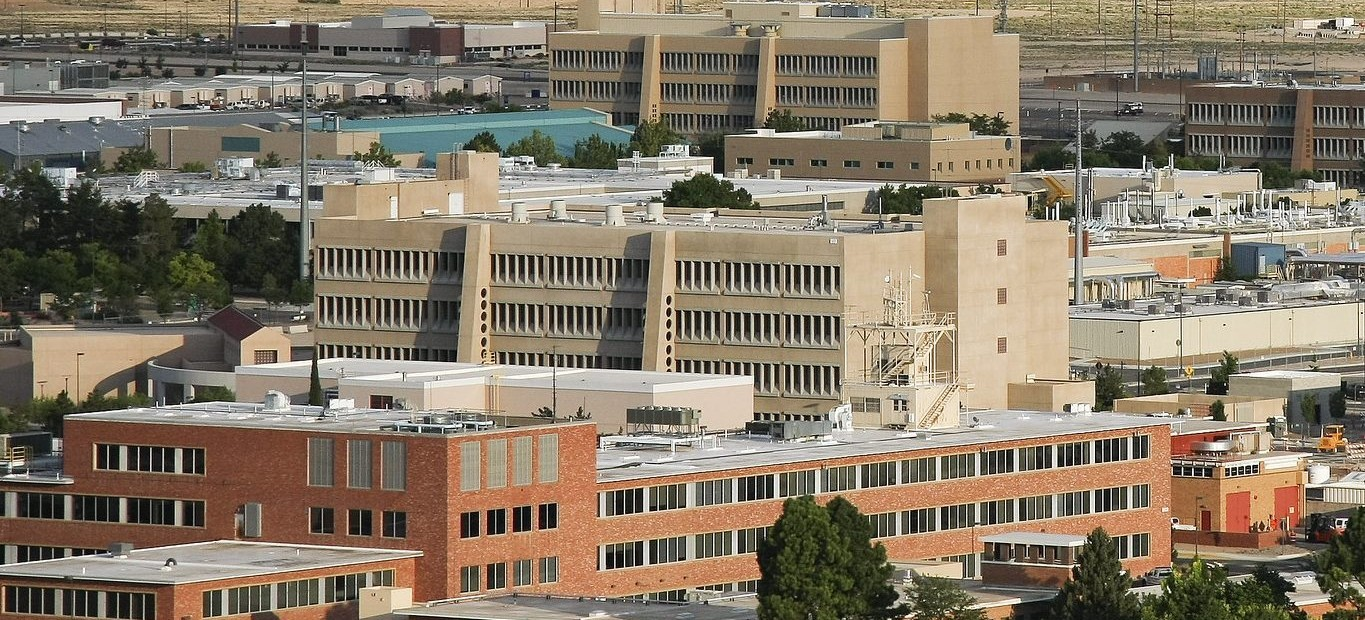
\includegraphics[width=\textwidth]{SNL4.jpg}
	\end{center}
	\vspace{0.4in}
	% --- UC Davis College of Engineering Logo ---
	\begin{center}
			
\includegraphics[width=3in]{COE.png}
	\end{center}
	\vspace{0.6in}
	% --- Project Title ---
	\begin{center}
		{\LARGE\bfseries\color{blue!70!black} \projecttitle}\\[12pt]
		{\large By the}\\[12pt]
		{\Large\bfseries \teamname}\\[24pt]
	\end{center}

	\vspace{0.4in}

	% --- Report Type ---
	\begin{center}
		{\large\bfseries TECHNICAL SUMMARY}
	\end{center}

	\vspace{0.4in}
	
	\begin{center}
		{\large SPONSORED BY \MakeUppercase{\sponsor},}\\
		{\large \MakeUppercase{\organization}}
	\end{center}

	\vfill

	% --- Submission Deadline ---
	\begin{center}
		{\large\bfseries \MakeUppercase{\duedate}}
	\end{center}

	\vspace{0.5in}
\end{titlepage}

\newpage
\thispagestyle{empty}
\vspace*{\fill}

% copyright page
\begin{center}

	{\large\bfseries Passive Temperature Compensation Device}\\[6pt]
	{\large Technical Summary}\\[24pt]

	\textcopyright\ 2026 by\\[6pt]
	Miguel Cuaycong, Jon Pizarro, Nicholas Metta,\\
	Isaiah Mathew, John Bodine, and Sam van der Veen\\[24pt]

	{\small
	
	EME 185: Mechanical Systems Design Project\\
	University of California, Davis\\[12pt]

	Advised by \instructor\ and\\
	\ta\\[24pt]

	\textit{All rights reserved. No part of this report may be reproduced}\\
	\textit{without consent from the authors, UC Davis,}\\
	\textit{or Sandia National Laboratories.}\\[24pt]

	}

\end{center}

\vspace*{\fill}

\newpage

\chapter*{\large{List of Acronyms}}

	\begin{longtable}{@{} l p{.75\textwidth} @{}}
		\toprule
		\textbf{Acronym} & \textbf{Definition} \\
		\midrule
		\endfirsthead

		\toprule
		\textbf{Acronym} & \textbf{Definition} \\
		\midrule
		\endhead

		\bottomrule
		\endfoot

		\bottomrule
		\endlastfoot

		Al      & Aluminum \\
		ALLV    & ALLVAR (negative-CTE alloy) \\
		ASME    & American Society of Mechanical Engineers \\
		BOM     & Bill of Materials \\
		CAD     & Computer-Aided Design \\
		CFD			& Computational Fluid Dynamics \\
		CNC			& Computer-Numerical Control \\
		COMSOL	& Computer Solution (numerical computing software) \\
		CTE     & Coefficient of Thermal Expansion \\
		DFMEA   & Design Failure Modes and Effects Analysis \\
		DIN			& Deutsches Institut für Normung (German Standardization Institute) \\
		DOF     & Degree of Freedom \\
		EBW     & Electron Beam Welding \\
		EDM     & Electrical Discharge Machining \\
		EME     & Engineering, Mechanical (course prefix) \\
		EN			& European Norm \\
		FEA			& Finite-Element Analysis \\
		FS      & Factor of Safety \\
		GTS			& Gas Transfer Systems (department at SNL) \\
		HEE			& Hydrogen Environmental Embrittlement \\
		HT			& Heat Transfer \\
		ID			& Inner Diameter \\
		Inc     & Inconel 718 \\
		Inv     & Invar 36 \\
		MBD			& Multi-Body Dynamics \\
		NASA    & National Aeronautics and Space Administration \\
		NPT			& National Pipe Taper \\
		OD			& Outer Diameter \\
		PI			& Pressure Indicator \\
		PPE			& Personal Protective Equipment \\
		PTCD    & Passive Temperature Compensation Device \\
		PTFE		& Polytetrafluoroethylene \\ 
		PVD			& Physical Vapor Deposition \\
		RPN			& Risk Priority Number \\
		RR      & Required Relationship \\
		SNL     & Sandia National Laboratories \\
		SS			& Stainless Steel \\
		TF      & Transfer Function \\
		TiCN		& Titanium Carbonitride \\
		UC Davis & University of California, Davis \\
		USA			& United States of America \\
	\end{longtable}
	% Don't worry about the error that appears here; the code should still compile

\newpage  % Start the body of the report on a fresh page

\setstretch{1.15}

\begin{abstract}

	Modern engineering constantly requires advances in technological precision and reliability.
	Sandia National Laboratories, a United States security and energy research facility, conducts many experiments that depend on submillimeter-precision flow control of high-pressure hydrogen gas.
	Their experiments are sensitive to temperature fluctuations; the flow must be adjusted for various reasons to compensate for these changes.
	However, power and space constraints prohibit the use of electronic power or computer control systems, and existing passive flow control solutions do not approach the size and precision these experiments require.
	
	Sandia commissioned the Noble Aggie Labs from the University of California, Davis to design a Passive Temperature Compensation Device (PTCD)
	that adjusts gas flow in response to external temperature changes without electronics.
	Engineered to contain and restrict hydrogen or a noble gas at up to 700 times atmospheric pressure,
	the PTCD maintains a pin-sized orifice with microscopic precision. 
	It does so with a novel square-orifice valve architecture that is driven by an external, bimetallic actuator.

	This report summarizes the design objectives and final selected architecture of the \device for a nontechnical audience.
	Full design justification, verification, and tools for iteration can be found in the Final Design Report by the same authors\cite{ref_finalDesignReport}.

\end{abstract}

\pagenumbering{arabic}

\chapter{Mission: Thermomechanical Flow Control}
\label{chap:intro}

	\section{Motivation}
	\label{sec:intro:motive}

		National security presents ceaseless challenges.
		Engineers must continually deliver advanced solutions to meet the ever-increasing demand for high-performance technology.
		Sandia National Laboratories, a United States security and energy research facility in Albuquerque, NM, executes this mission.
		Their development of cutting-edge defense technology and scientific research protects American citizens and sojourners alike against sophisticated threats
		and pioneers advancements in energy efficiency and sustainability.
		Resolving the nation's most challenging security issues, Sandia must employ every means to maintain a competitive edge in the international theater.
		Even a small improvement in the capacity or reliability of a larger integrated system can deliver a key advantage.

		Sandia's Gas Transfer Systems team, based in Livermore, CA, develops specialized tools that are used in any of the myriad projects undertaken at the Lab.
		Many of their developmental experiments require precision flow control of high-pressure $\text{H}_{\text{2}}$ gas.
		Downstream conditions are sensitive to environmental temperature fluctuations and must either be tightly controlled or extensively post-processed.
		Gas flow provided to the test article must be restricted by an orifice, no more than a few hundred micrometers across, that closes as the ambient air temperature rises.
		Electrically-powered valves accomplish this well.
		However, lab technicians often cannot actively control flow in these experiments due to power, personnel, or space constraints.
		They would require a fully passive valve, one that could control the flow of high-pressure gas across a wide temperature range with extreme precision.
		Passive temperature-compensating devices exist on the market, but none approach the size or performance characteristics needed.
		Thermostatic actuators\cite{ref_ASHRAE_thermostatic, ref_Vernet_1938} control air-conditioning dampers or regulate the temperature of engine coolant, being especially common in the mid-20th century.
		These respond to and regulate their internal fluid temperature, rather than adjusting the internal flow in response to the ambient external conditions,
		and are designed for low-pressure, loose-tolerance applications.
		Thermal louvers and thermostatic bypass valves\cite{ref_Bugby_2021, ref_Ralphs_2024, ref_Ralphs_2026} passively regulate delicate satellite equipment at the size and precision Sandia requires
		but switch on and off to compensate for the binary thermal extremes of space rather than delivering a continuous output.
		Therefore, despite this design foundation, a passive, precise valve that continuously manipulates fluid flow without responding to its internal conditions would prove a novel and challenging exercise.

	\section{Objectives}
	\label{sec:intro:objectives}

		Thus it is that Sandia National Labs (SNL, aka the ``sponsor'') commissioned the Noble Aggie Labs, a mechanical design team at the University of California, Davis and the authors of this paper,
		to design a Passive Temperature Compensation Device (\device, Figure~\ref{fig:conceptual})\cite{ref_sandiaprompt} that precisely controls experimental conditions by passively responding to temperature changes.
		Being allotted six months to develop a full design package and test a virtual prototype, the Noble Aggie Labs provided Sandia with 

		\begin{figure}[h]
			\centering
			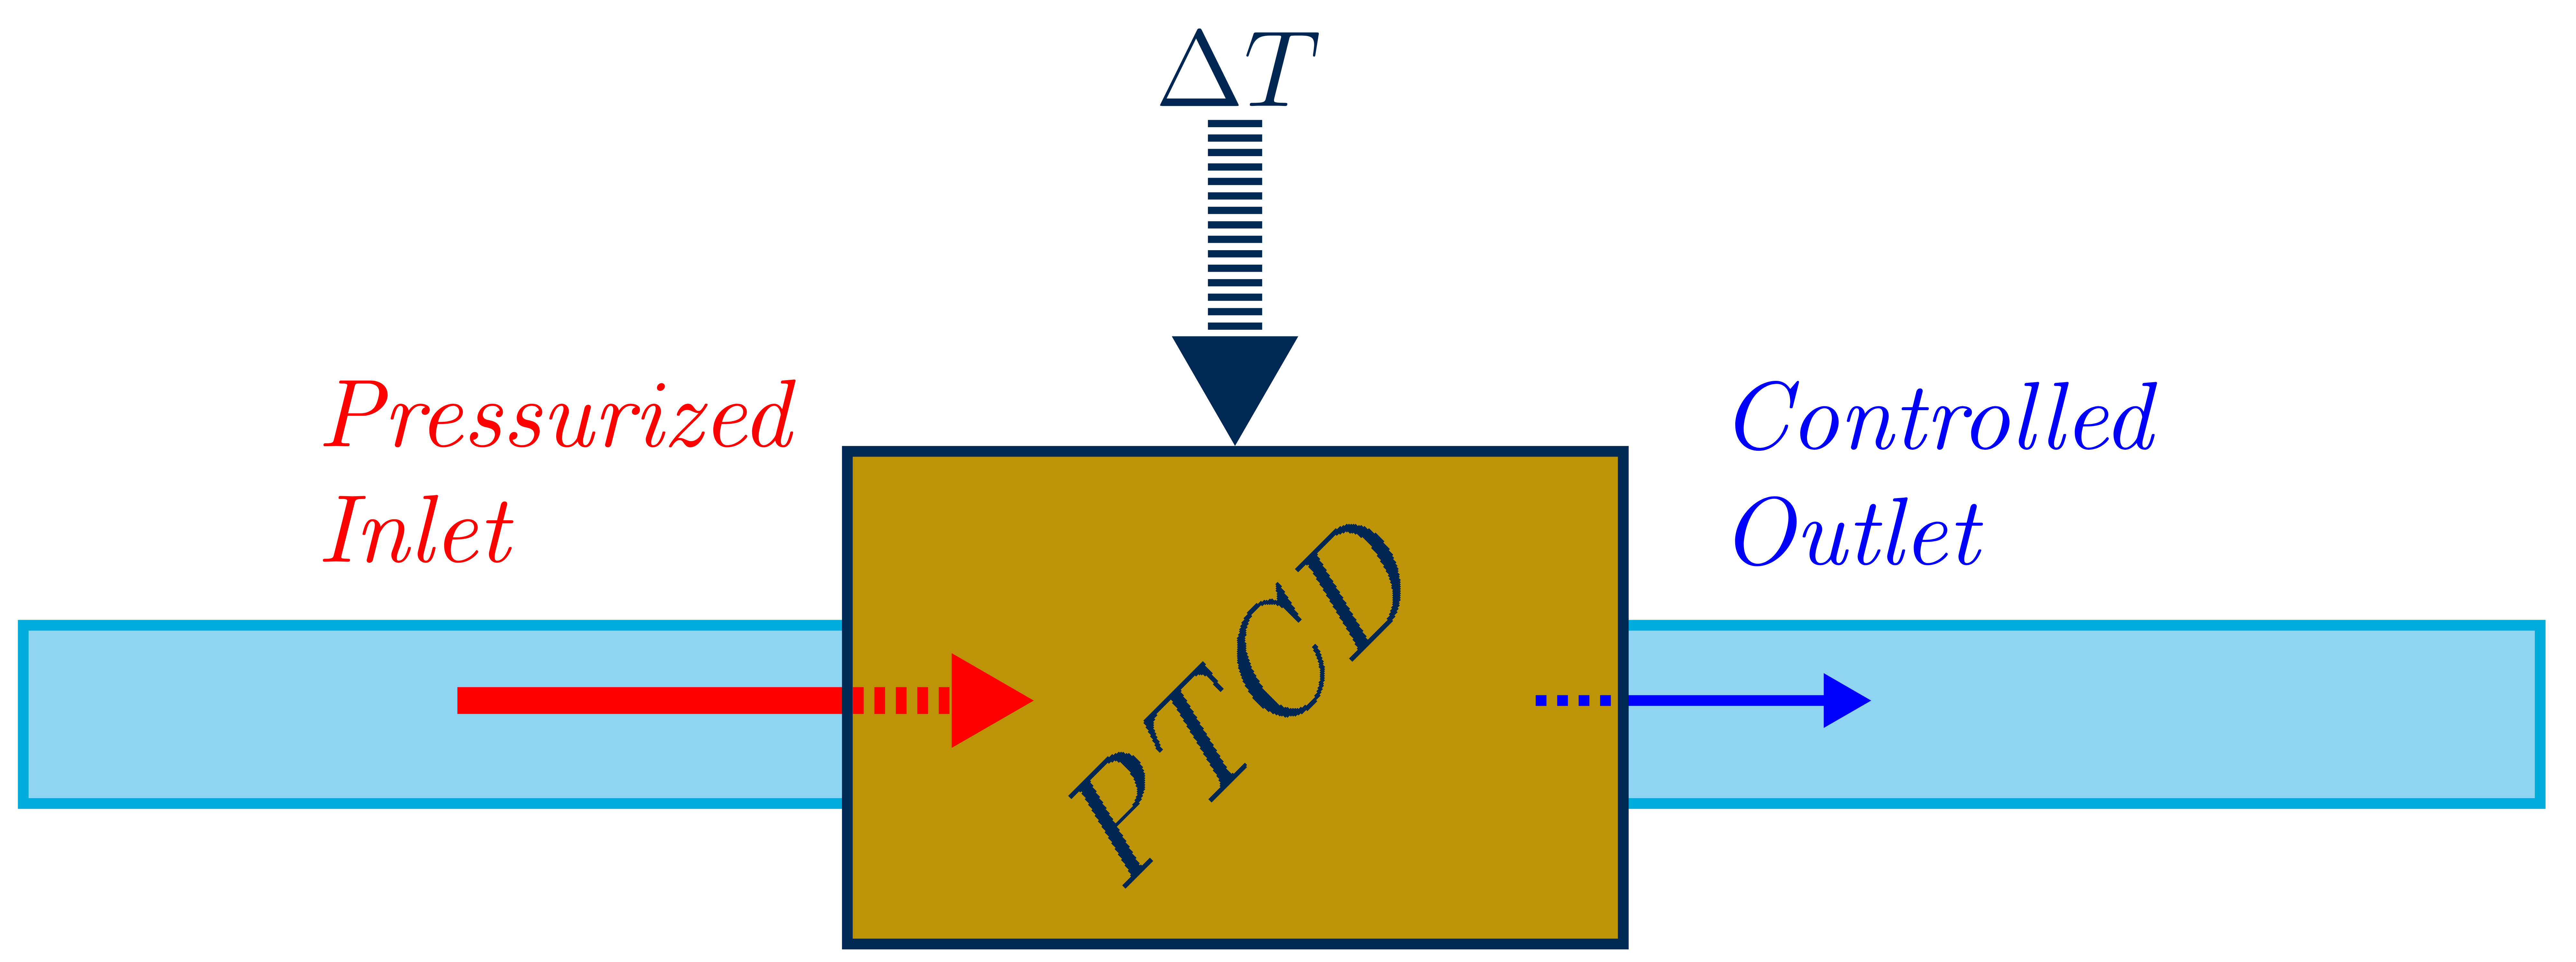
\includegraphics[height=1.8in]{conceptual.png}
			\caption{Conceptual diagram of the \device}
			\label{fig:conceptual}
		\end{figure}

		\vspace{1em}
		\begin{figure}[h]
			\centering
			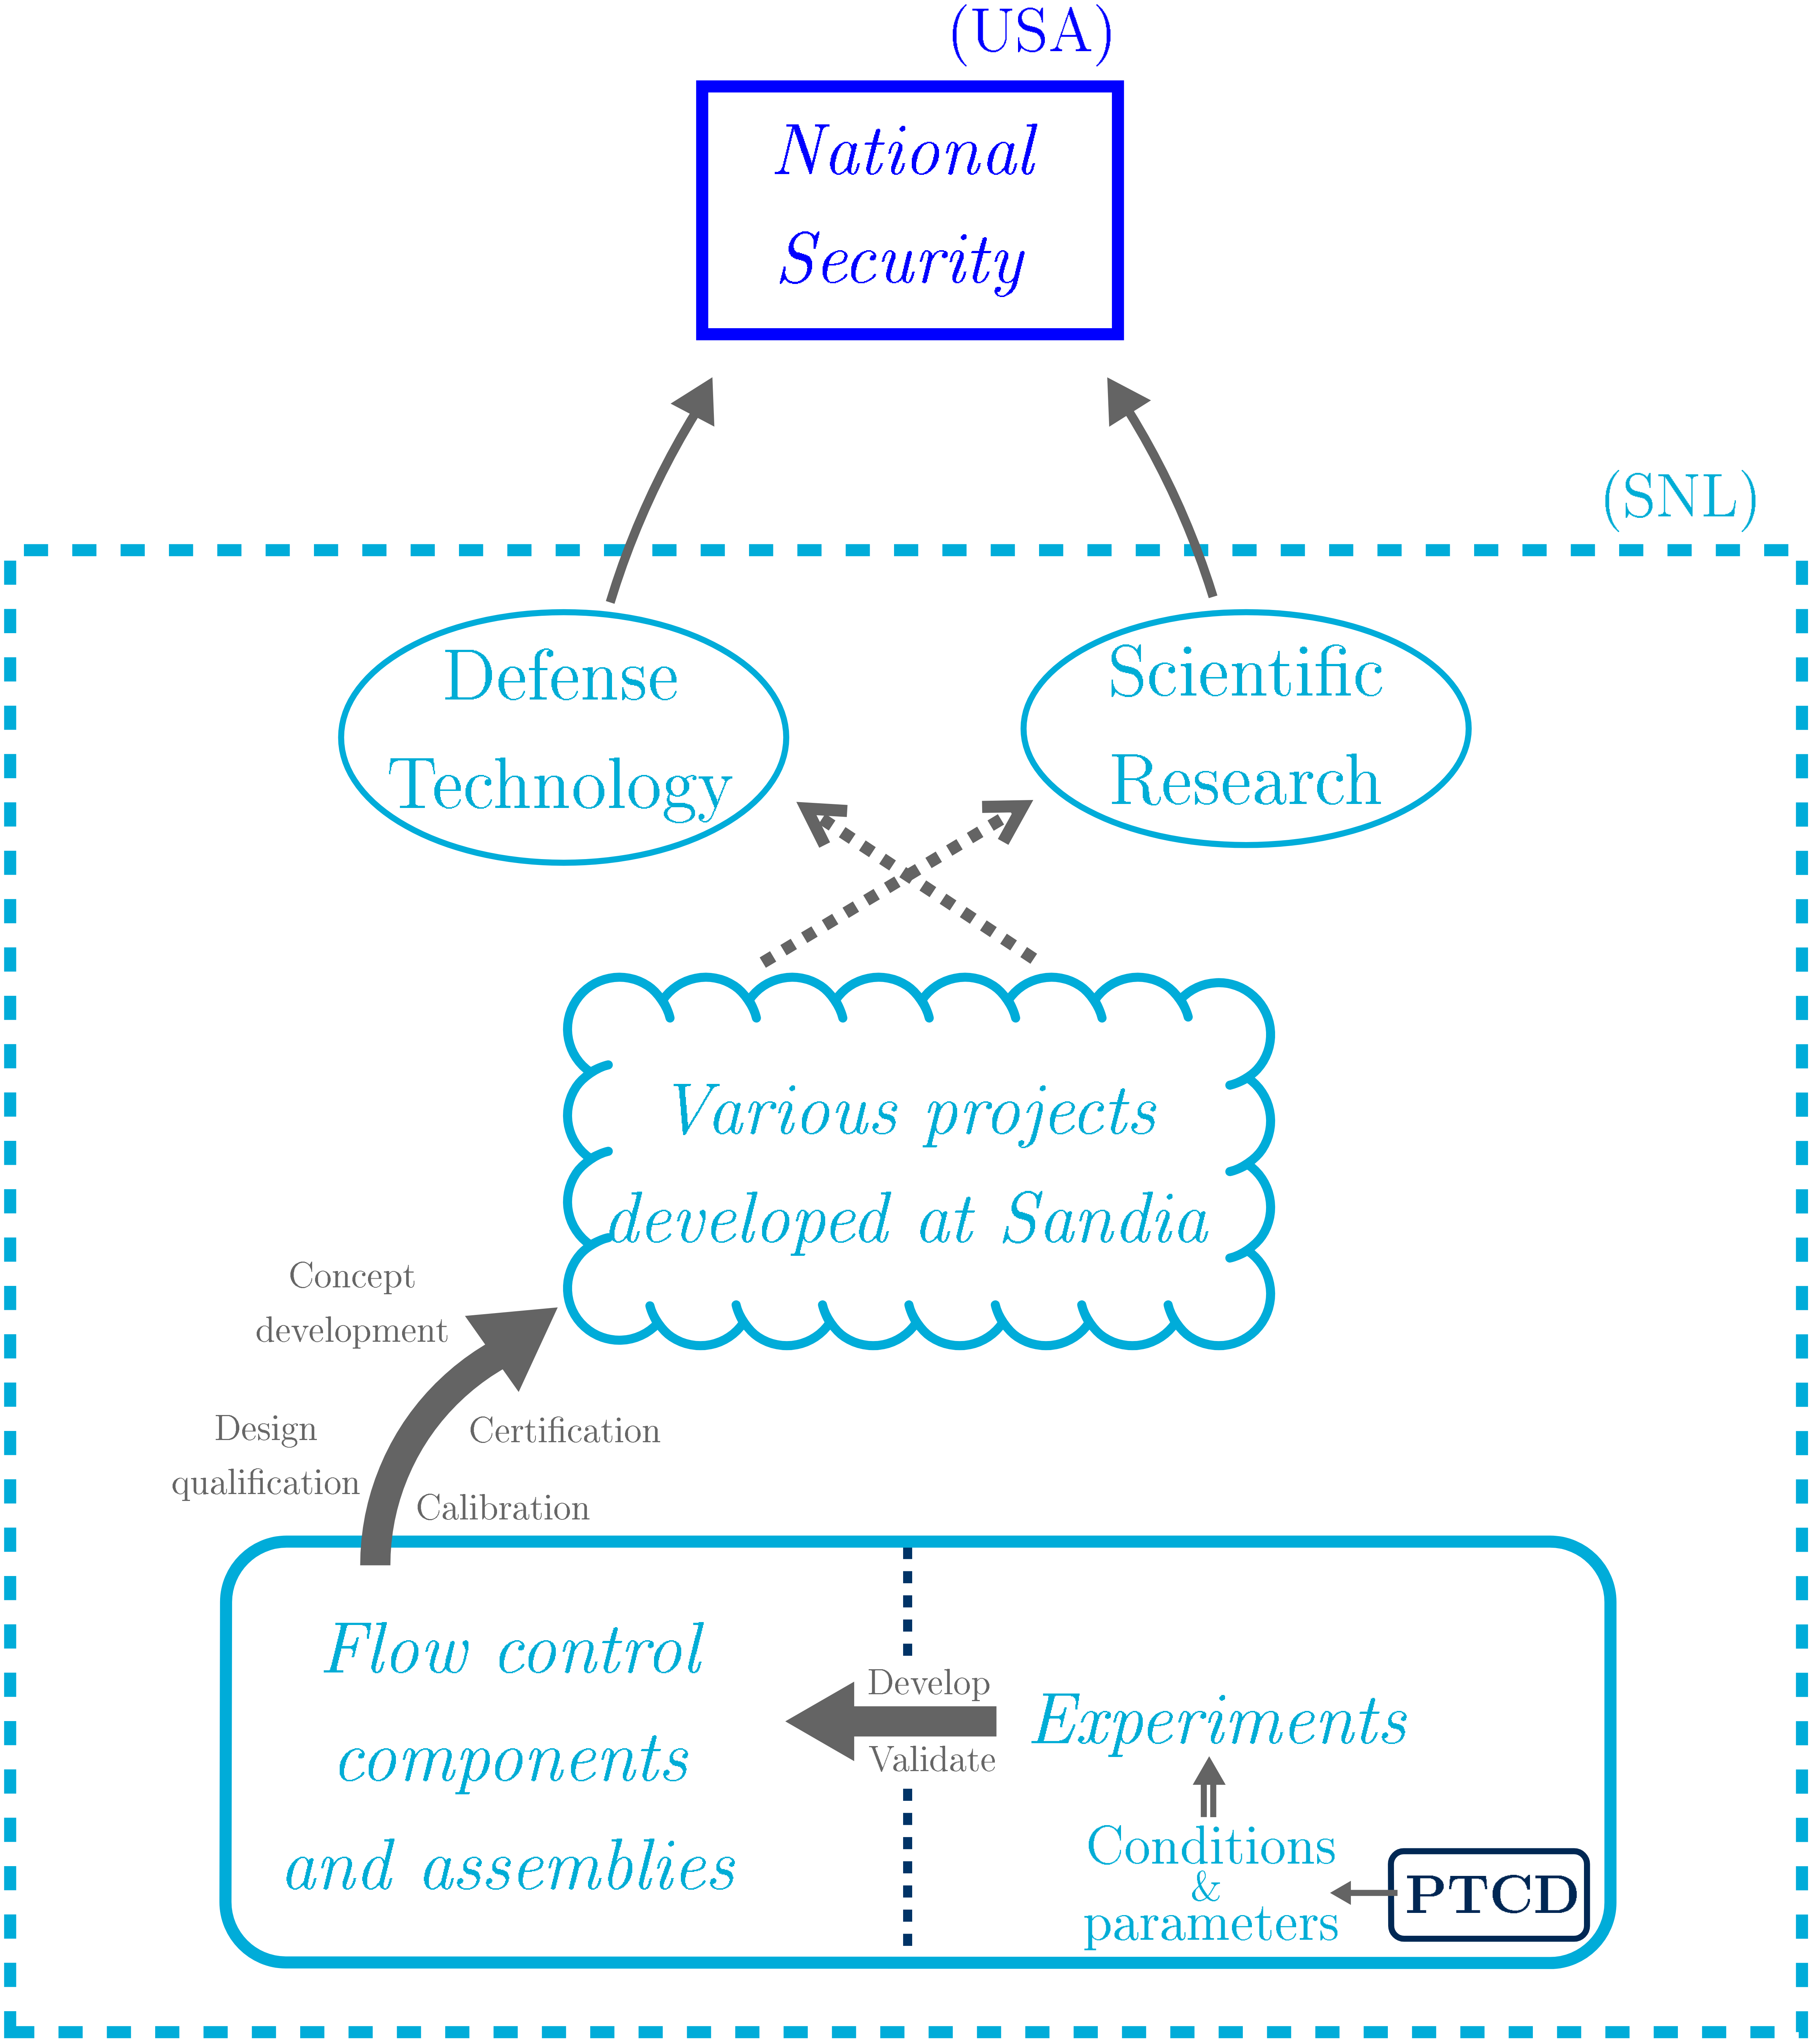
\includegraphics[width=.75\textwidth]{SNL_role.png}
			\caption{Downstream customer diagram}
			\label{fig:app_SNL}
		\end{figure}

		Figure~\ref{fig:app_SNL} illustrates the \device's niche role. Sandia National Labs develops ``science and technology to resolve the nation's most challenging security issues''\cite{ref_SNL}.
		Sandia's Gas Transfer Systems (GTS) team, whose scope is pictured in the lower nested rectangle, develops flow control components and assemblies
		that Sandia then uses for the concept development, design qualification, certification, and calibration of some of their projects.
		GTS develops and validates these components through a series of tightly controlled experiments; the \device\ will serve as part of the experimental setup
		to compensate for temperature fluctuations, eliminating the need for powered flow-control components or data correction
		and ultimately improving the reliability of the science and technology Sandia produces.

	\section{System Requirements}
	\label{sec:intro:req}

		As stipulated by Sandia, the \device\ must passively restrict the flow of hydrogen or a noble gas at any temperature
		and up to \SI{69}{\mega\pascal} (690 atmospheres) internal pressure
		such that its effective orifice diameter (the diameter of a circular orifice of equivalent area) is directly proportional to the external air temperature,
		shrinks as the temperature increases, and meets the following setpoints:

		\begin{align}
			\Dcold \label{eq:coldBoundary} \\
			\Dref \label{eq:DTref} \\
			\Dhot \label{eq:hotBoundary}
		\end{align}

		This results in the Required Relationship shown in Figure~\ref{fig:RR}. The device must also be smaller than $(\SI{10}{\centi\meter})^3$ on all sides
		(small enough to fit in one's hand). It must be strong enough withstand the extreme internal pressure and must prevent the diffusion of hydrogen, which permeates through many flexible materials.
		The \device\ must maintain an orifice smaller than the tip of a ballpoint pen to within 10--20 \si{\micro\meter} (no more than the width of a human hair\cite{ref_NIH}) from its setpoint
		between the thermal extremes of the surface temperature of Antarctica on a winter's day and a running engine block.
		This small valve must thermomechanically control a submillimeter orifice to a micron-scale tolerance, maintaining a linear output across a wide temperature range under extreme pressures.

		\begin{figure}[h]
			\centering
			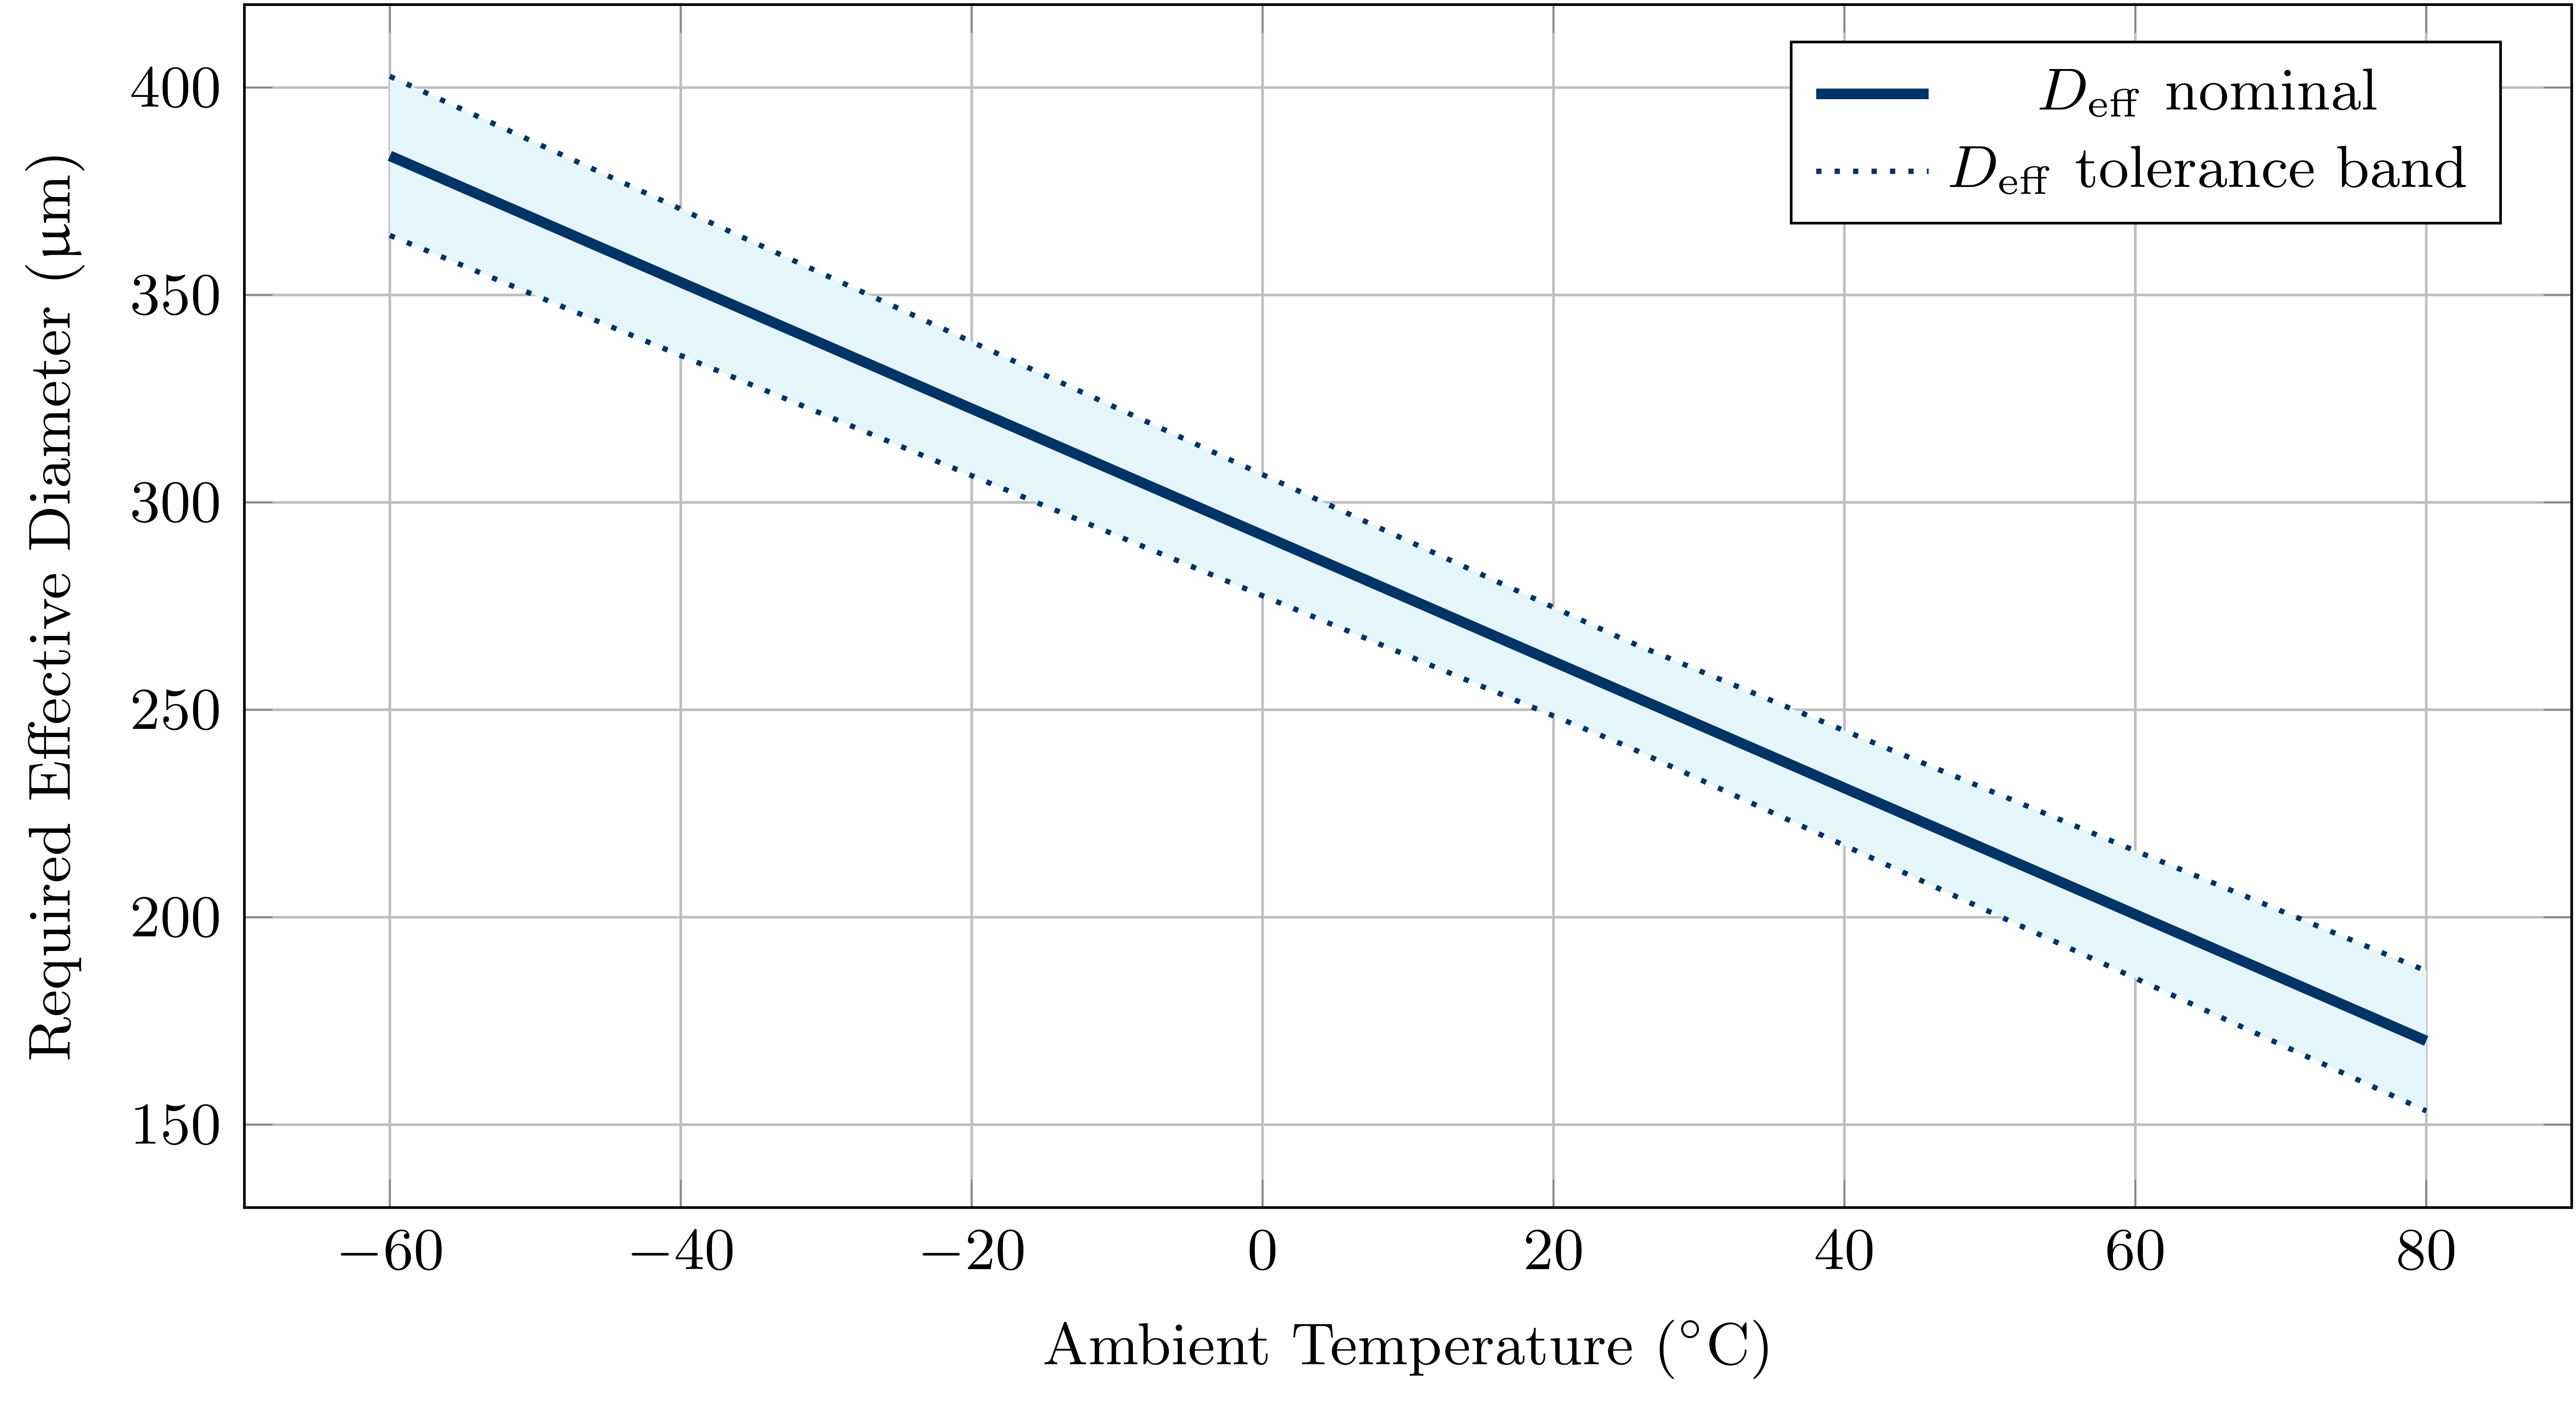
\includegraphics[width=\textwidth]{RR.png}
			\caption{Required Relationship tolerance window}
			\label{fig:RR}
		\end{figure}

\chapter{Final Design of the \device}
\label{chap:design}

	After six months of development, the Noble Aggie Labs delivered a complete design package\cite{ref_finalDesignReport} to Sandia's engineers,
	who will continue to revise the design until it is fit to be manufactured and tested.

\chapter{Final Design of the \device}

	\section{System Architecture Overview}
	\label{sec:design:overview}

		The \device\, pictured in Figure~\ref{fig:reveal}, uses two independent subsystems, combining proven technology with novel innovations to accomplish a formerly impossible mission.
		combines proven, aerospace-grade designs and materials with a novel valve architecture to convert temperature fluctuations into precise thermomechanical displacement
		then convert that motion into flow restriction.

		The \device\ contains and seals high-pressure hydrogen gas and delivers precise thermomechanical actuation with proven, aerospace-grade technology.
		It also introduces a novel variable-diamond orifice that overcomes several weaknesses of existing valve architectures.
		The device comprises a valve assembly, with a threaded housing, orifice components, and associated hermetic seals; and an actuator assembly, with a bimetallic architecture and calibration system.
		The full assembly is pictured in Figures~\ref{fig:reveal}, \ref{fig:mainIsometric}, and \ref{fig:mainExploded}.

		\vspace{1em}
		\begin{figure}[H]
			\centering
			% 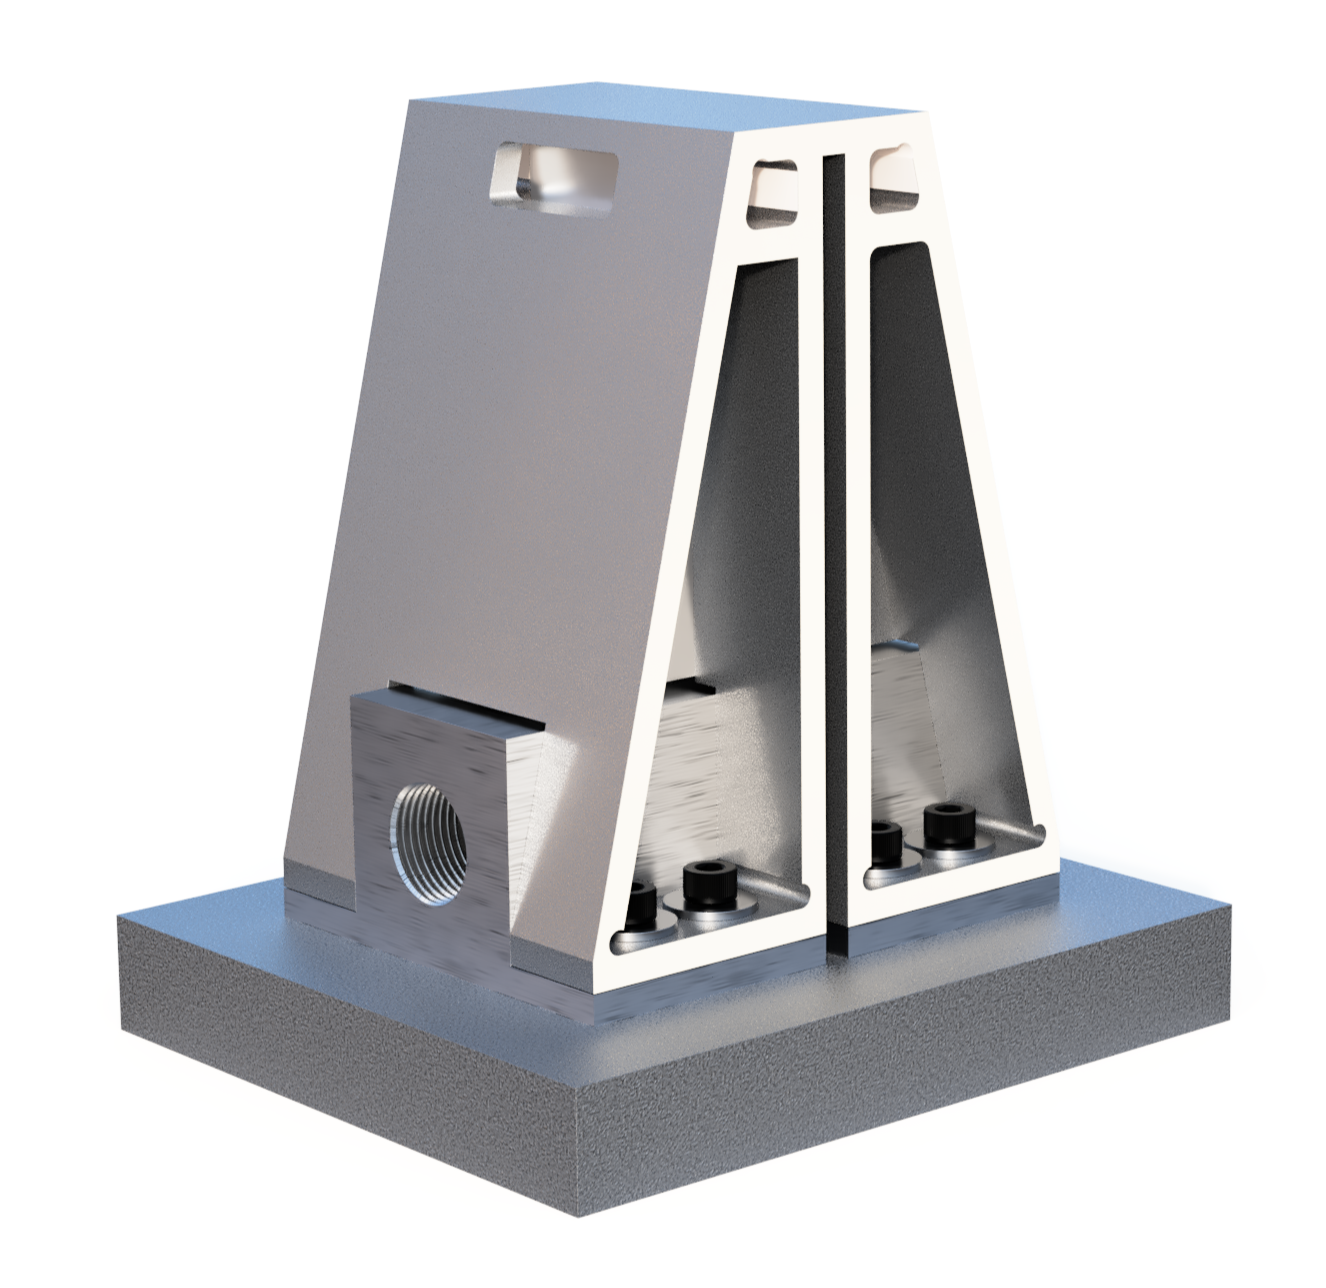
\includegraphics[height=\dimexpr\textheight-\pagetotal-3\baselineskip\relax, width=\textwidth, keepaspectratio]{Complete_Assembly_Render.png}
			\includegraphics[height=\dimexpr\textheight-\pagetotal-3\baselineskip\relax, width=\textwidth, keepaspectratio]{reveal_qual.png}
			\caption{The Passive Temperature Compensation Device}
			\label{fig:reveal}
		\end{figure}
		\newpage
		\begin{figure}[H]
			\begin{minipage}{.49\textwidth}
				\centering
				% 
\includegraphics[width=.85\textwidth]{CompleteAssemblyExploded.png}
				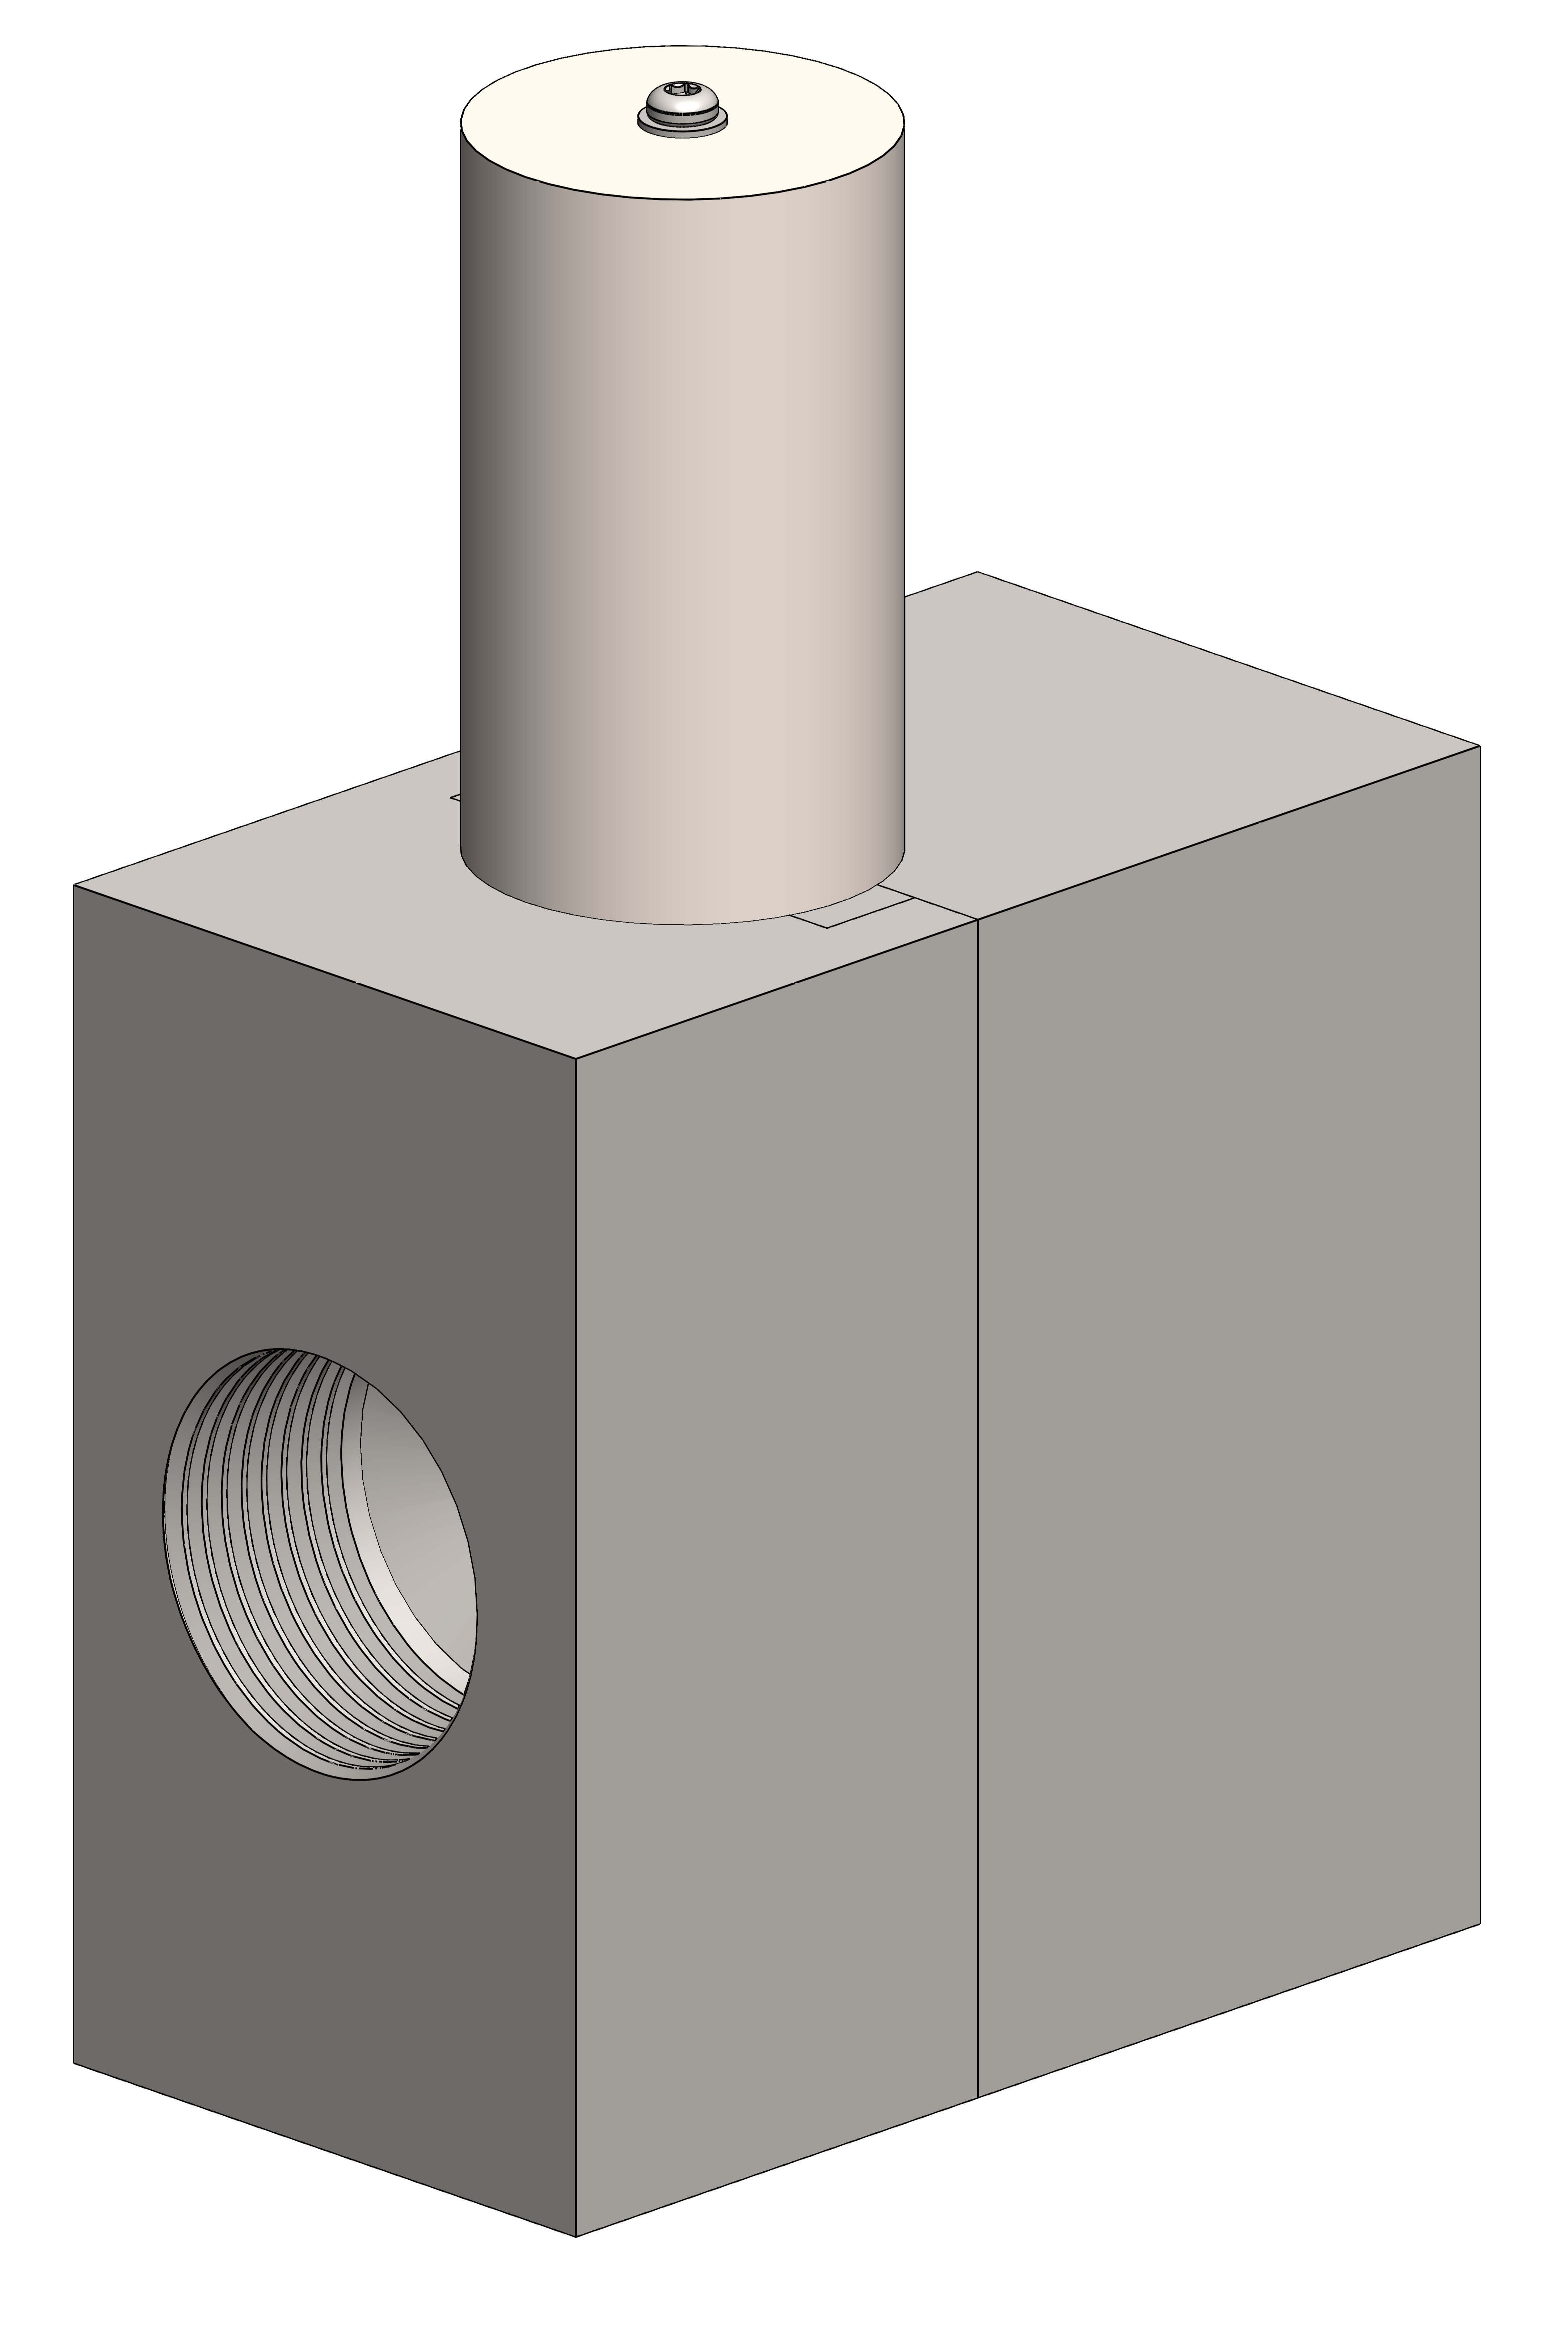
\includegraphics[width=.75\textwidth]{PTCD.png}
				\caption{Complete assembly isometric view}
				\label{fig:mainIsometric}
			\end{minipage}
			\hfill
			\begin{minipage}{.49\textwidth}
				\centering
				\includegraphics[width=.75\textwidth]{exp_qual.png}
				\caption{Complete assembly exploded view}
				\label{fig:mainExploded}
			\end{minipage}
		\end{figure}

		\begin{wrapfigure}{l}{.3\textwidth}
			\centering
			
\includegraphics[height=2in]{orifice.png}
			\caption{Orifice geometry}
			\label{fig:orifice}
		\end{wrapfigure}

		The valve orifice at the heart of the PTCD comprises two plates with identical square holes cut at 45$^\circ$ angles.
		One plate is fixed to the valve housing; the other is free to move vertically as driven by the valve stem.\footnote{This report will refer to the hole in the mobile Valve Orifice part and the hole in the fixed Housing as the leading and trailing orifice, respectively.}
		The two square holes lie flush against one another and are vertically offset such that only a small square opening appears between the valve inlet and its outlet. 
		If the two holes were circles, they would resemble a Venn diagram; thus, as pictured in Figure~\ref{fig:orifice}, the diamond-shaped overlap between these squares constitutes the valve orifice. 
		The lower (blue) square is cut into the central moving plate such that as the valve stem drives the plate downwards, the orifice (the gray overlap region) constricts.
		
		A bimetallic actuator is fixed above the housing and welded to the valve stem; it drives the central orifice as it responds to temperature changes.
		The outer material, ALLVAR, shrinks when heated, while the inner material, aluminum, expands.
		Thus, as pictured in Figure~\ref{fig:active_diagram}, as the ambient temperature increases, the actuator drives the valve stem downwards, shrinking the orifice. 
		As the temperature decreases, the actuator pulls the stem back up, opening the orifice again. Across the total design temperature range, the actuator expands \SI{267}{\micro\meter}, driving the valve an equal distance.

		\begin{figure}[H]
			\centering
			\begin{minipage}{.45\textwidth}
				\centering
				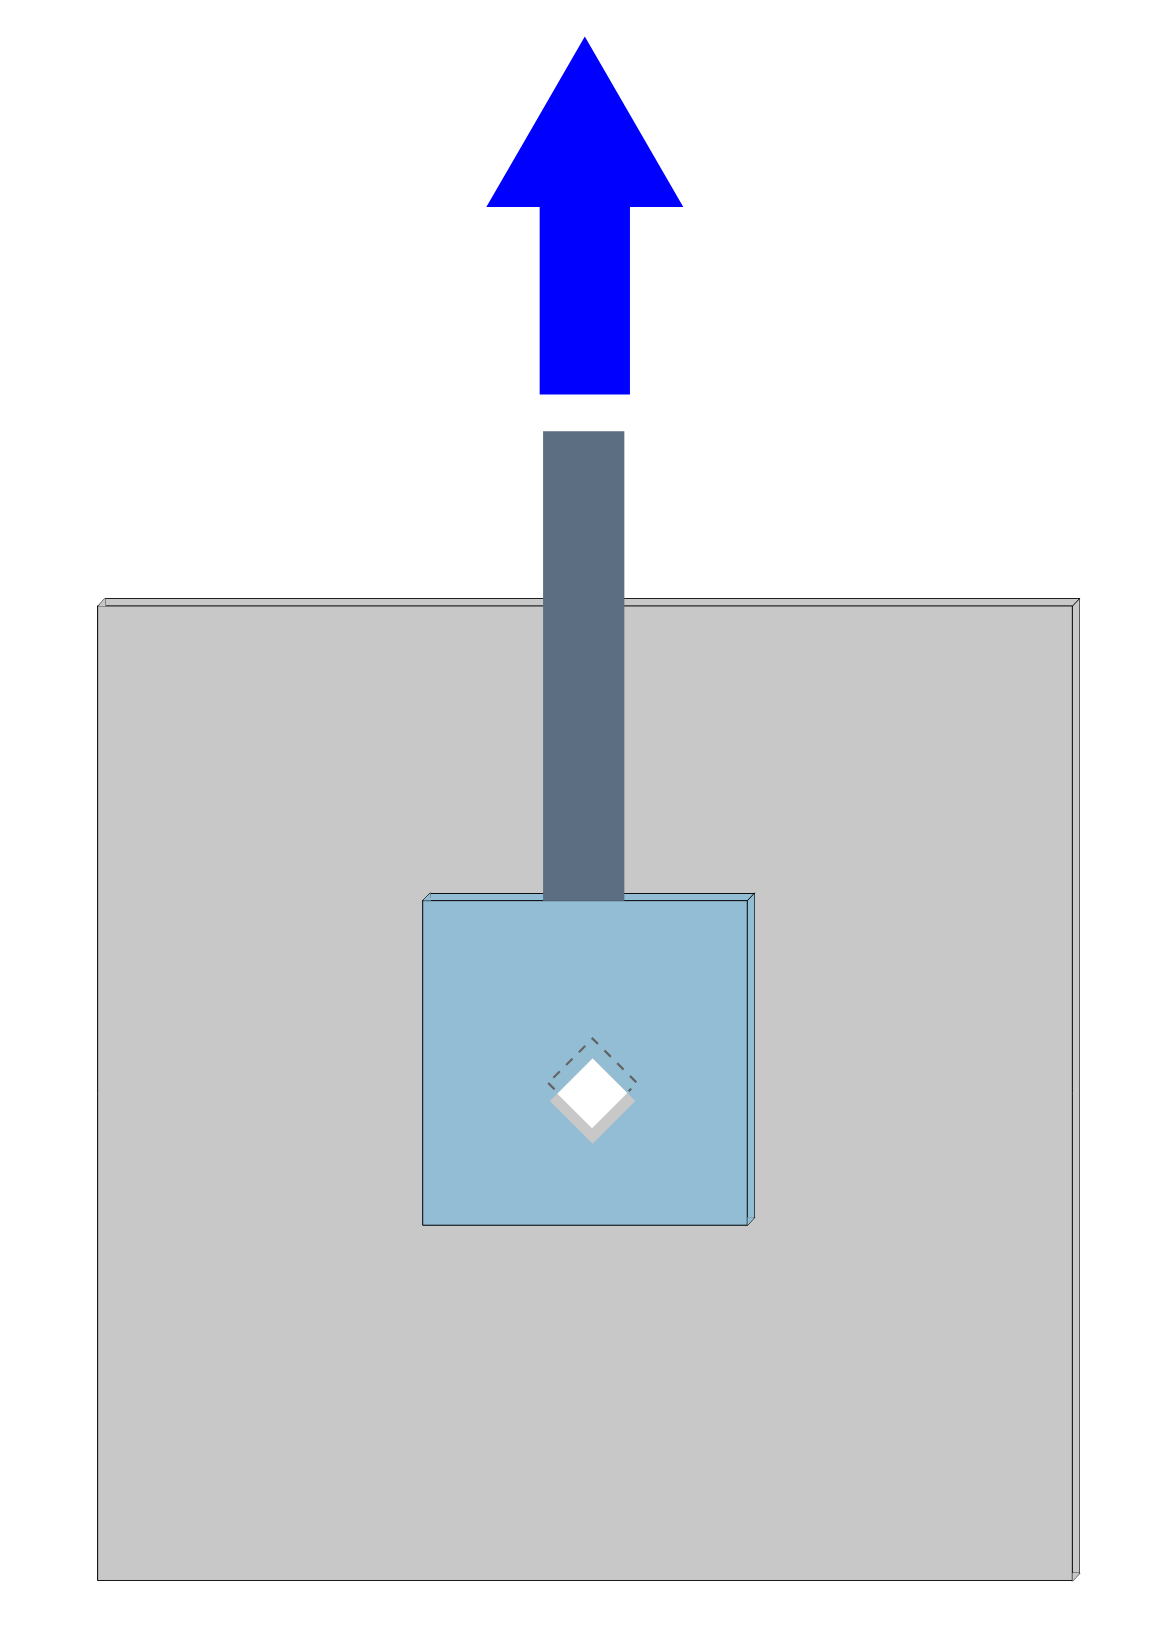
\includegraphics[width=.7\textwidth]{active_cold.png}
				\subcaption{Cooling actuation}
				\label{fig:active_cold}
			\end{minipage}
			\hfill
			\begin{minipage}{.45\textwidth}
				\centering
				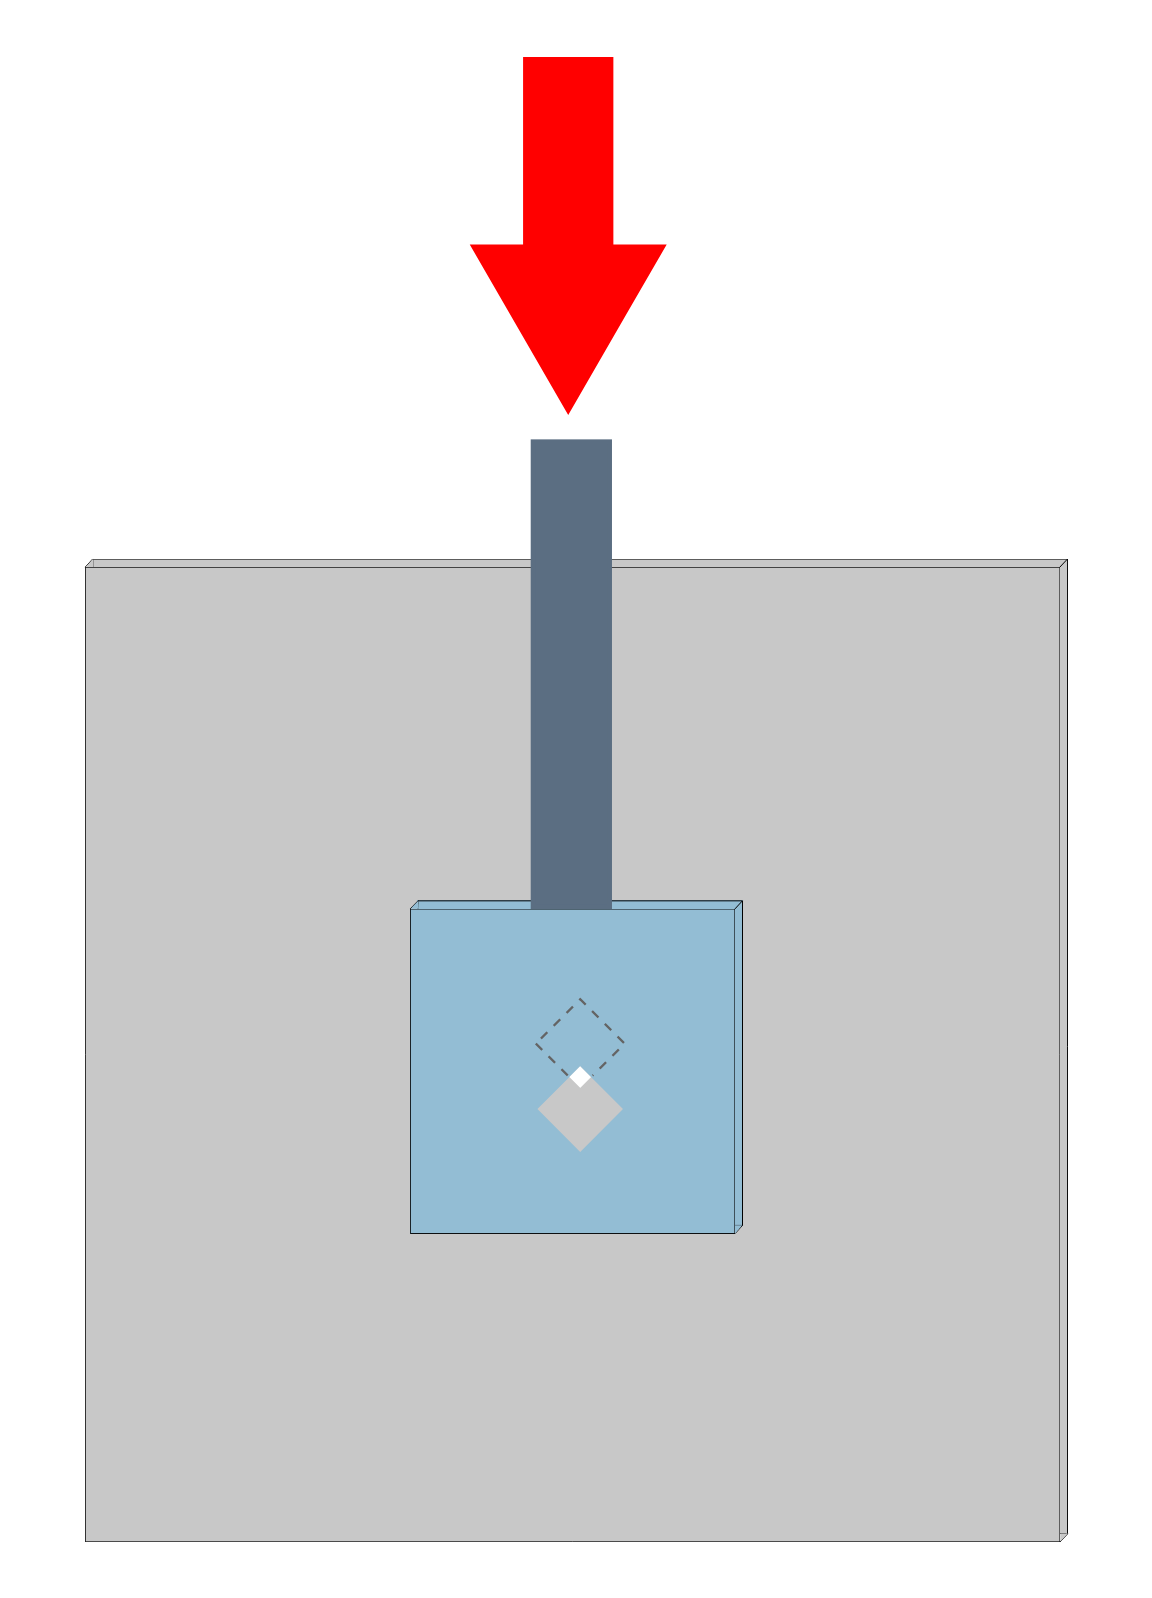
\includegraphics[width=.7\textwidth]{active_hot.png}
				\subcaption{Heating actuation}
				\label{fig:active_hot}
			\end{minipage}
			\caption{Mechanism of the \device}
			\label{fig:active_diagram}
		\end{figure}

		\subsection{Valve Subsystem}
		\label{subsec:design:overview:valve}

			\begin{wrapfigure}{l}{.32\textheight} % .32\textheight is the width, but the image is roughly square
				\centering
				% 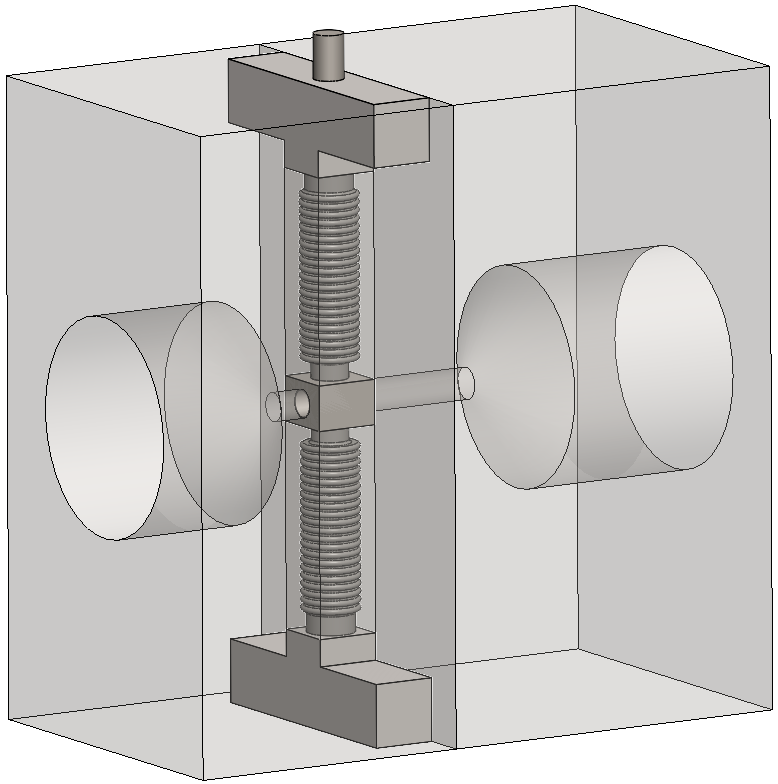
\includegraphics[height=.4\textheight]{Valve_full.png}
				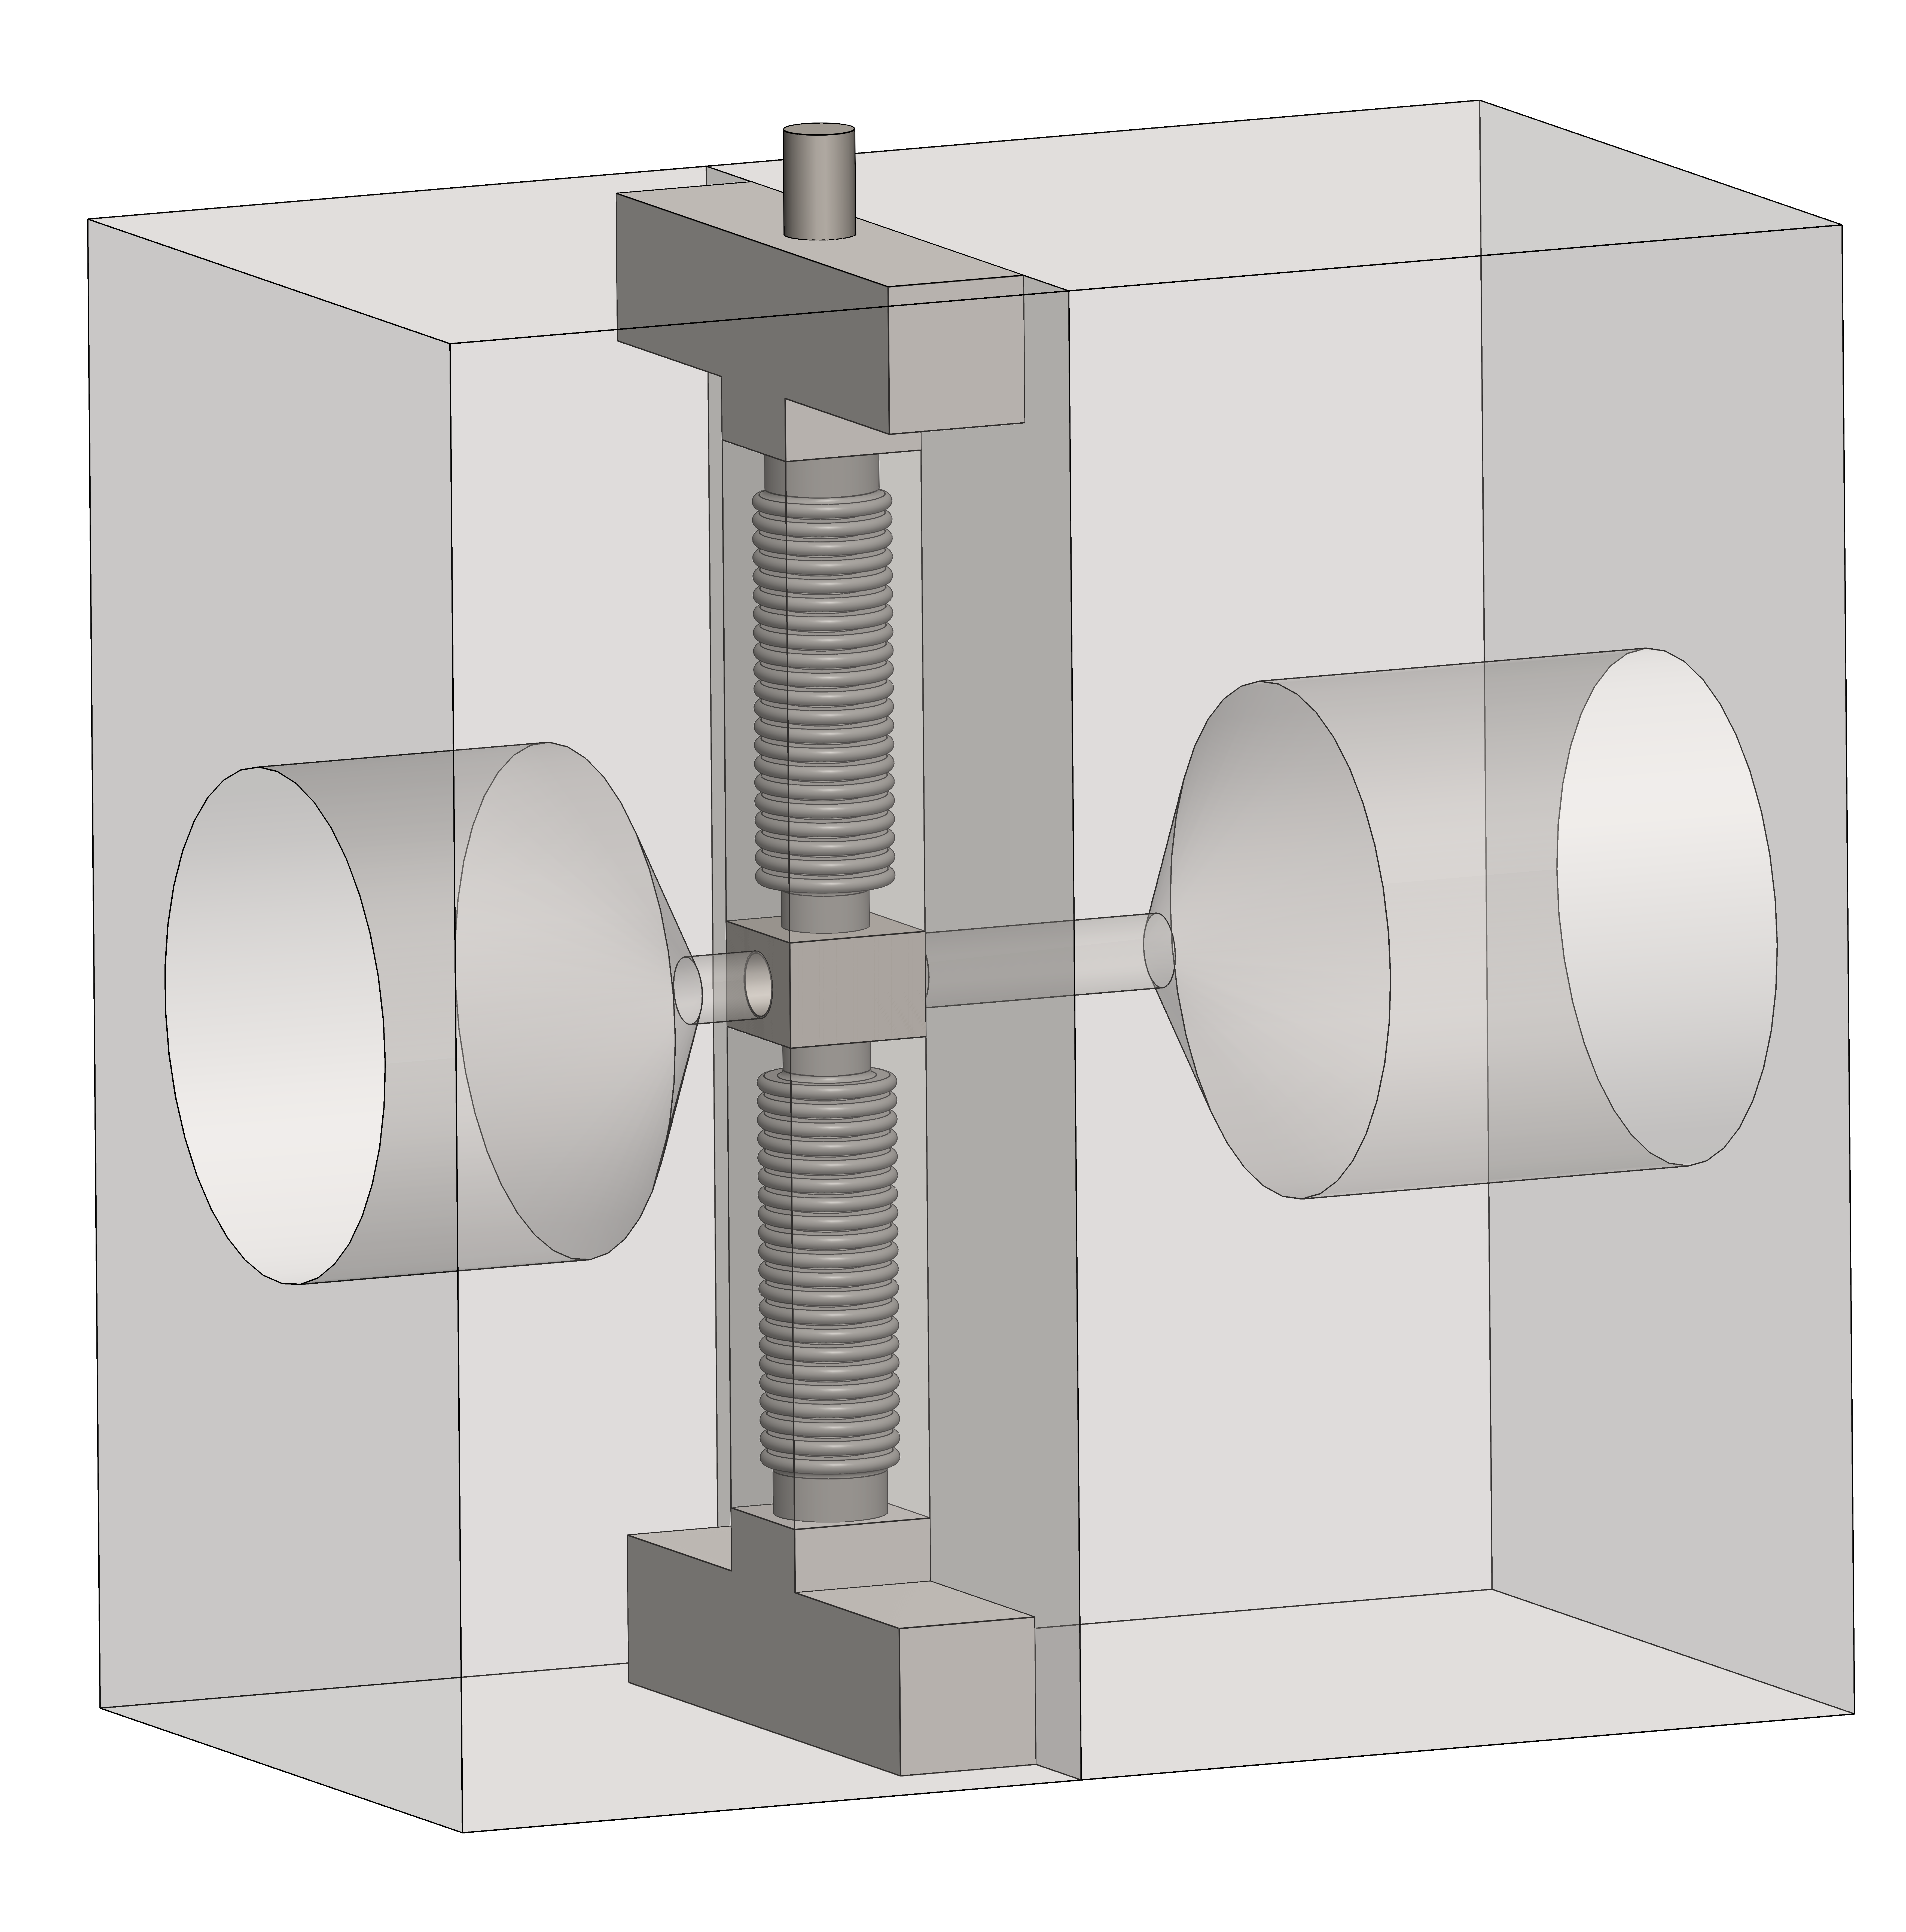
\includegraphics[height=.3\textheight]{Valve_full_qual.png}
				\caption{Valve subsystem}
				\label{fig:valve_full}
			\end{wrapfigure}

			The valve subsystem (Figures~\ref{fig:valve_full}, \ref{fig:valve_exploded}, \ref{fig:valve_ID}) contains the high-pressure gas and restricts its flow, only allowing gas to exit through its small internal orifice.
			Its housing is coupled to stainless steel pipes by a test engineer and provides the structural support necessary to hold the internal pressure.
			The leading-orifice component nests between four walls and slides vertically within the assembly.
			Attached is the valve stem, welded to and driven by the actuator.
			This housing penetration is hermetically sealed by a bellows. A corresponding valve stem-bellows pair extends through the bottom of the housing to balance the resultant pressure forces.

			\begin{figure}[H]
				\begin{minipage}{.49\textwidth}
					\centering
					% 
\includegraphics[width=\textwidth]{Valve_exploded.png}
					\includegraphics[width=\textwidth]{Valve_exploded_qual.png}
					\caption{Valve subsystem exploded view}
					\label{fig:valve_exploded}
				\end{minipage}
				\hfill
				\begin{minipage}{.49\textwidth}
					\centering
					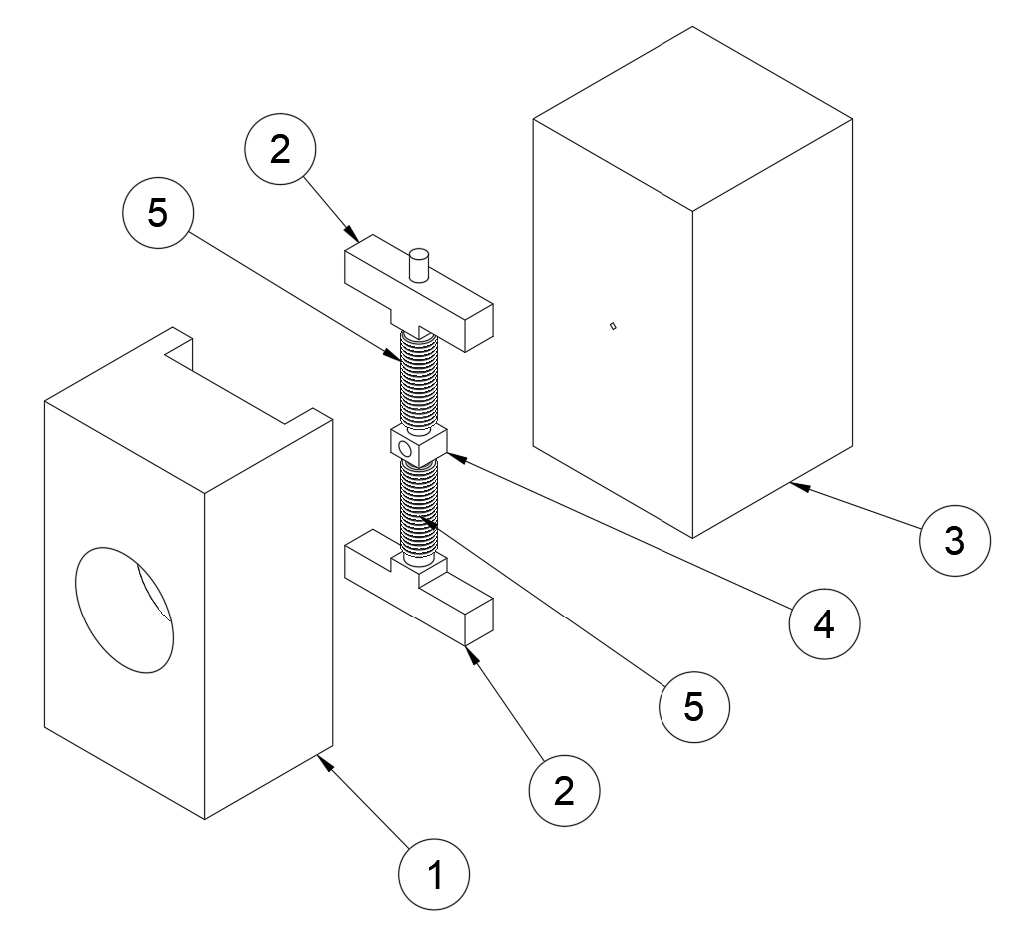
\includegraphics[width=\textwidth]{Valve_ID.png}
					\caption{Valve subsystem part identification}
					\label{fig:valve_ID}
				\end{minipage}
			\end{figure}

			\begin{wrapfigure}{l}{2.5in}
				\centering
				% 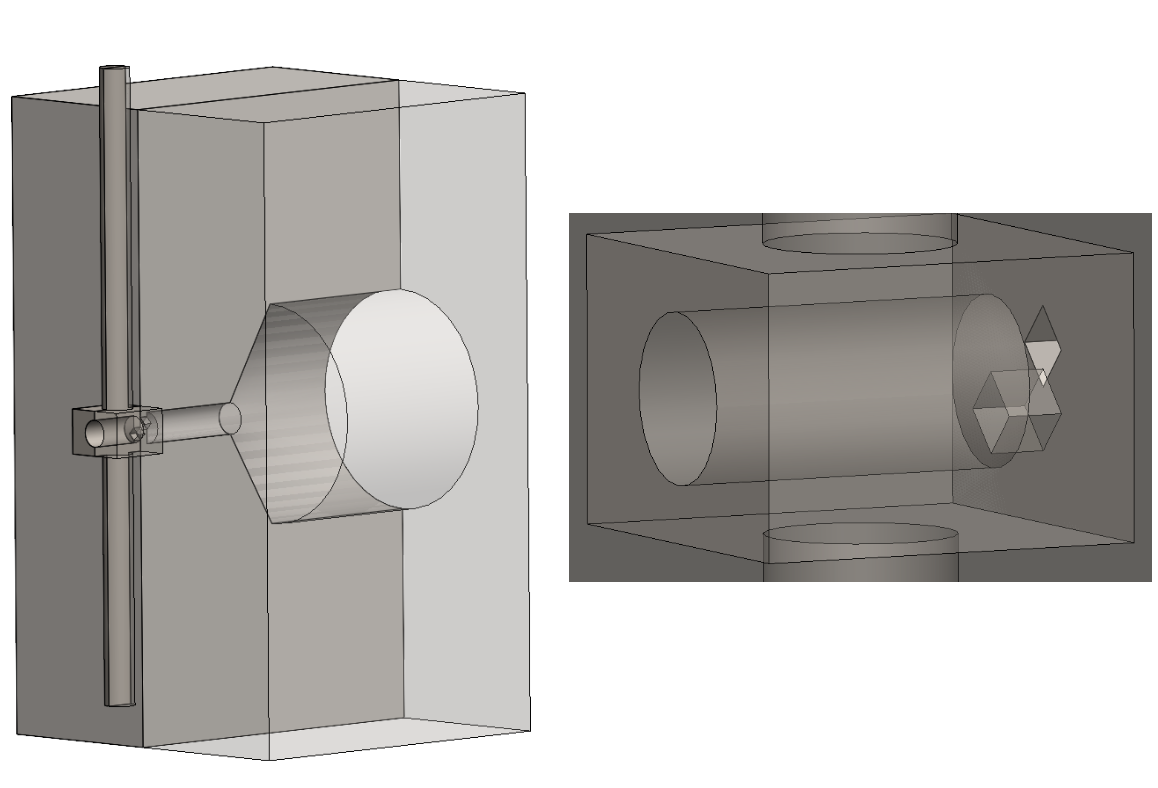
\includegraphics[width=.8\textwidth]{orif_assem.png}
				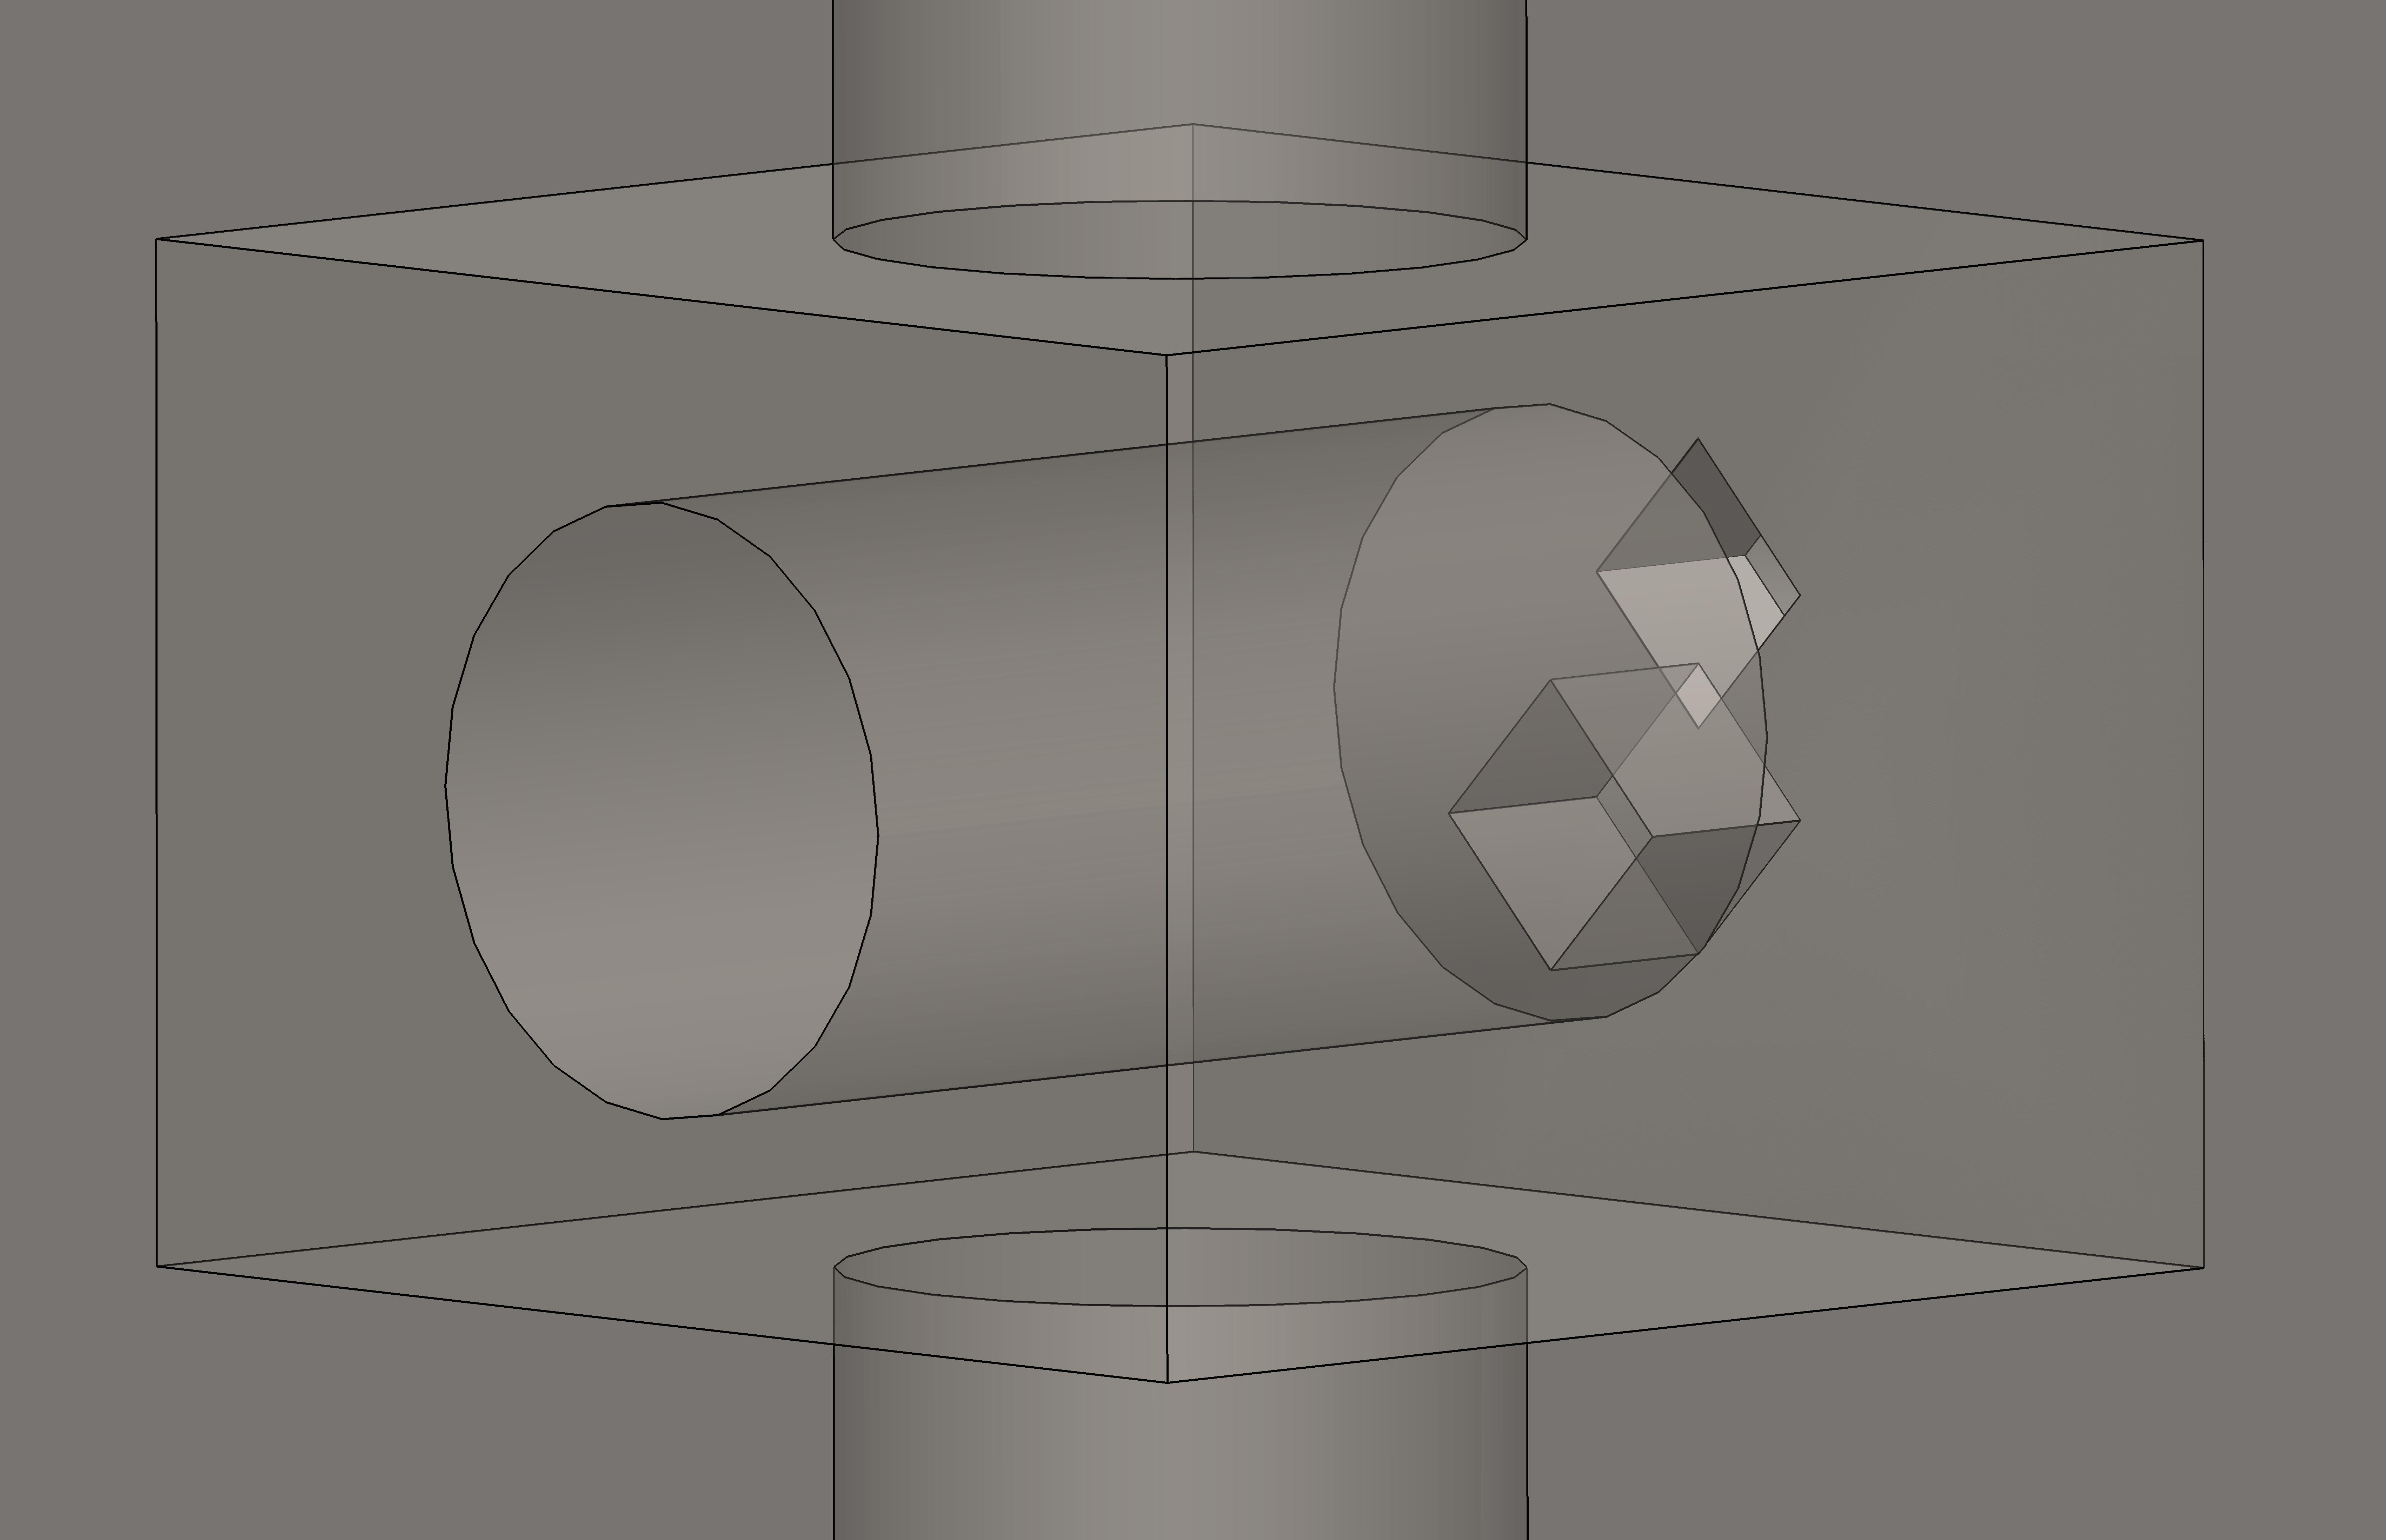
\includegraphics[width=2.5in]{orif_assem_right_qual.png}
				\caption{Orifice assembly}
				\label{fig:orif_assem}
			\end{wrapfigure}

			The Valve Orifice (4) comprises the leading orifice hole near its center.
			The actuator drives its motion via the upper valve stem so that it moves freely up and down while the other parts remain fixed.
			It lies flush against the Housing Outlet (3), which comprises the trailing orifice hole and directs low-pressure gas out of the assembly through a pipe threaded into its rear.
			Together, these comprise the \device's orifice, shown in Figure~\ref{fig:orif_assem}.

			Lateral and longitudinal movement of the Valve Orifice are constrained by the Housing Inlet (1), which presses it against the face of the Outlet and restricts all motion to the vertical degree of freedom.
			The inlet and outlet butt together, leaving enough space in its central channel for the Valve Orifice to fit snugly between four walls.

			Two Housing Center pieces (2) plug the remaining gaps.
			They contain holes for the valve stems to slide through, guiding their motion.
			To hermetically seal these holes, a bellows (5) is welded between the Valve Orifice and each Housing Center.
			As the centerpiece moves up and down, the flexible bellows extend and contract, allowing for flexible, sealed penetration of the housing.
			The housing center and bellows are inserted as in Figure~\ref{fig:V1_bellows}.

			\newpage

			\begin{figure}[H]
				\begin{minipage}{4.5in}
			Figure~\ref{fig:cut_zooms} shows the orifice in full assembly.
			The leading orifice on the moving piece is positioned below the trailing orifice as prescribed in Figure~\ref{fig:orifice}.

					\medskip
					All components of the valve assembly are joined by Electron Beam Weld (EBW), a precise method to attach flush faces against one another and nearly perfectly fuse them together.

					\medskip
					All machined parts are made of Invar 36\cite{ref_Invar_1897, ref_Invar_1920}, a Ni-Fe alloy renowned for its exceptionally low thermal expansion,
					ensuring high thermal stability under the expected temperature fluctuations.
				\end{minipage}
			\hfill
				\begin{minipage}{1.9in}
				\centering
				% 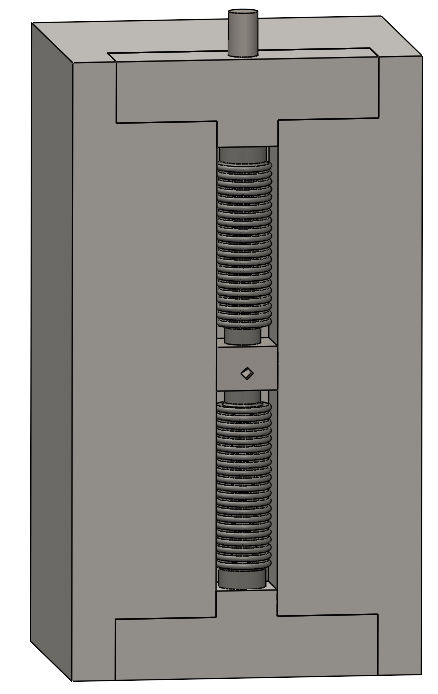
\includegraphics[height=4in]{V1_bellows.png}
				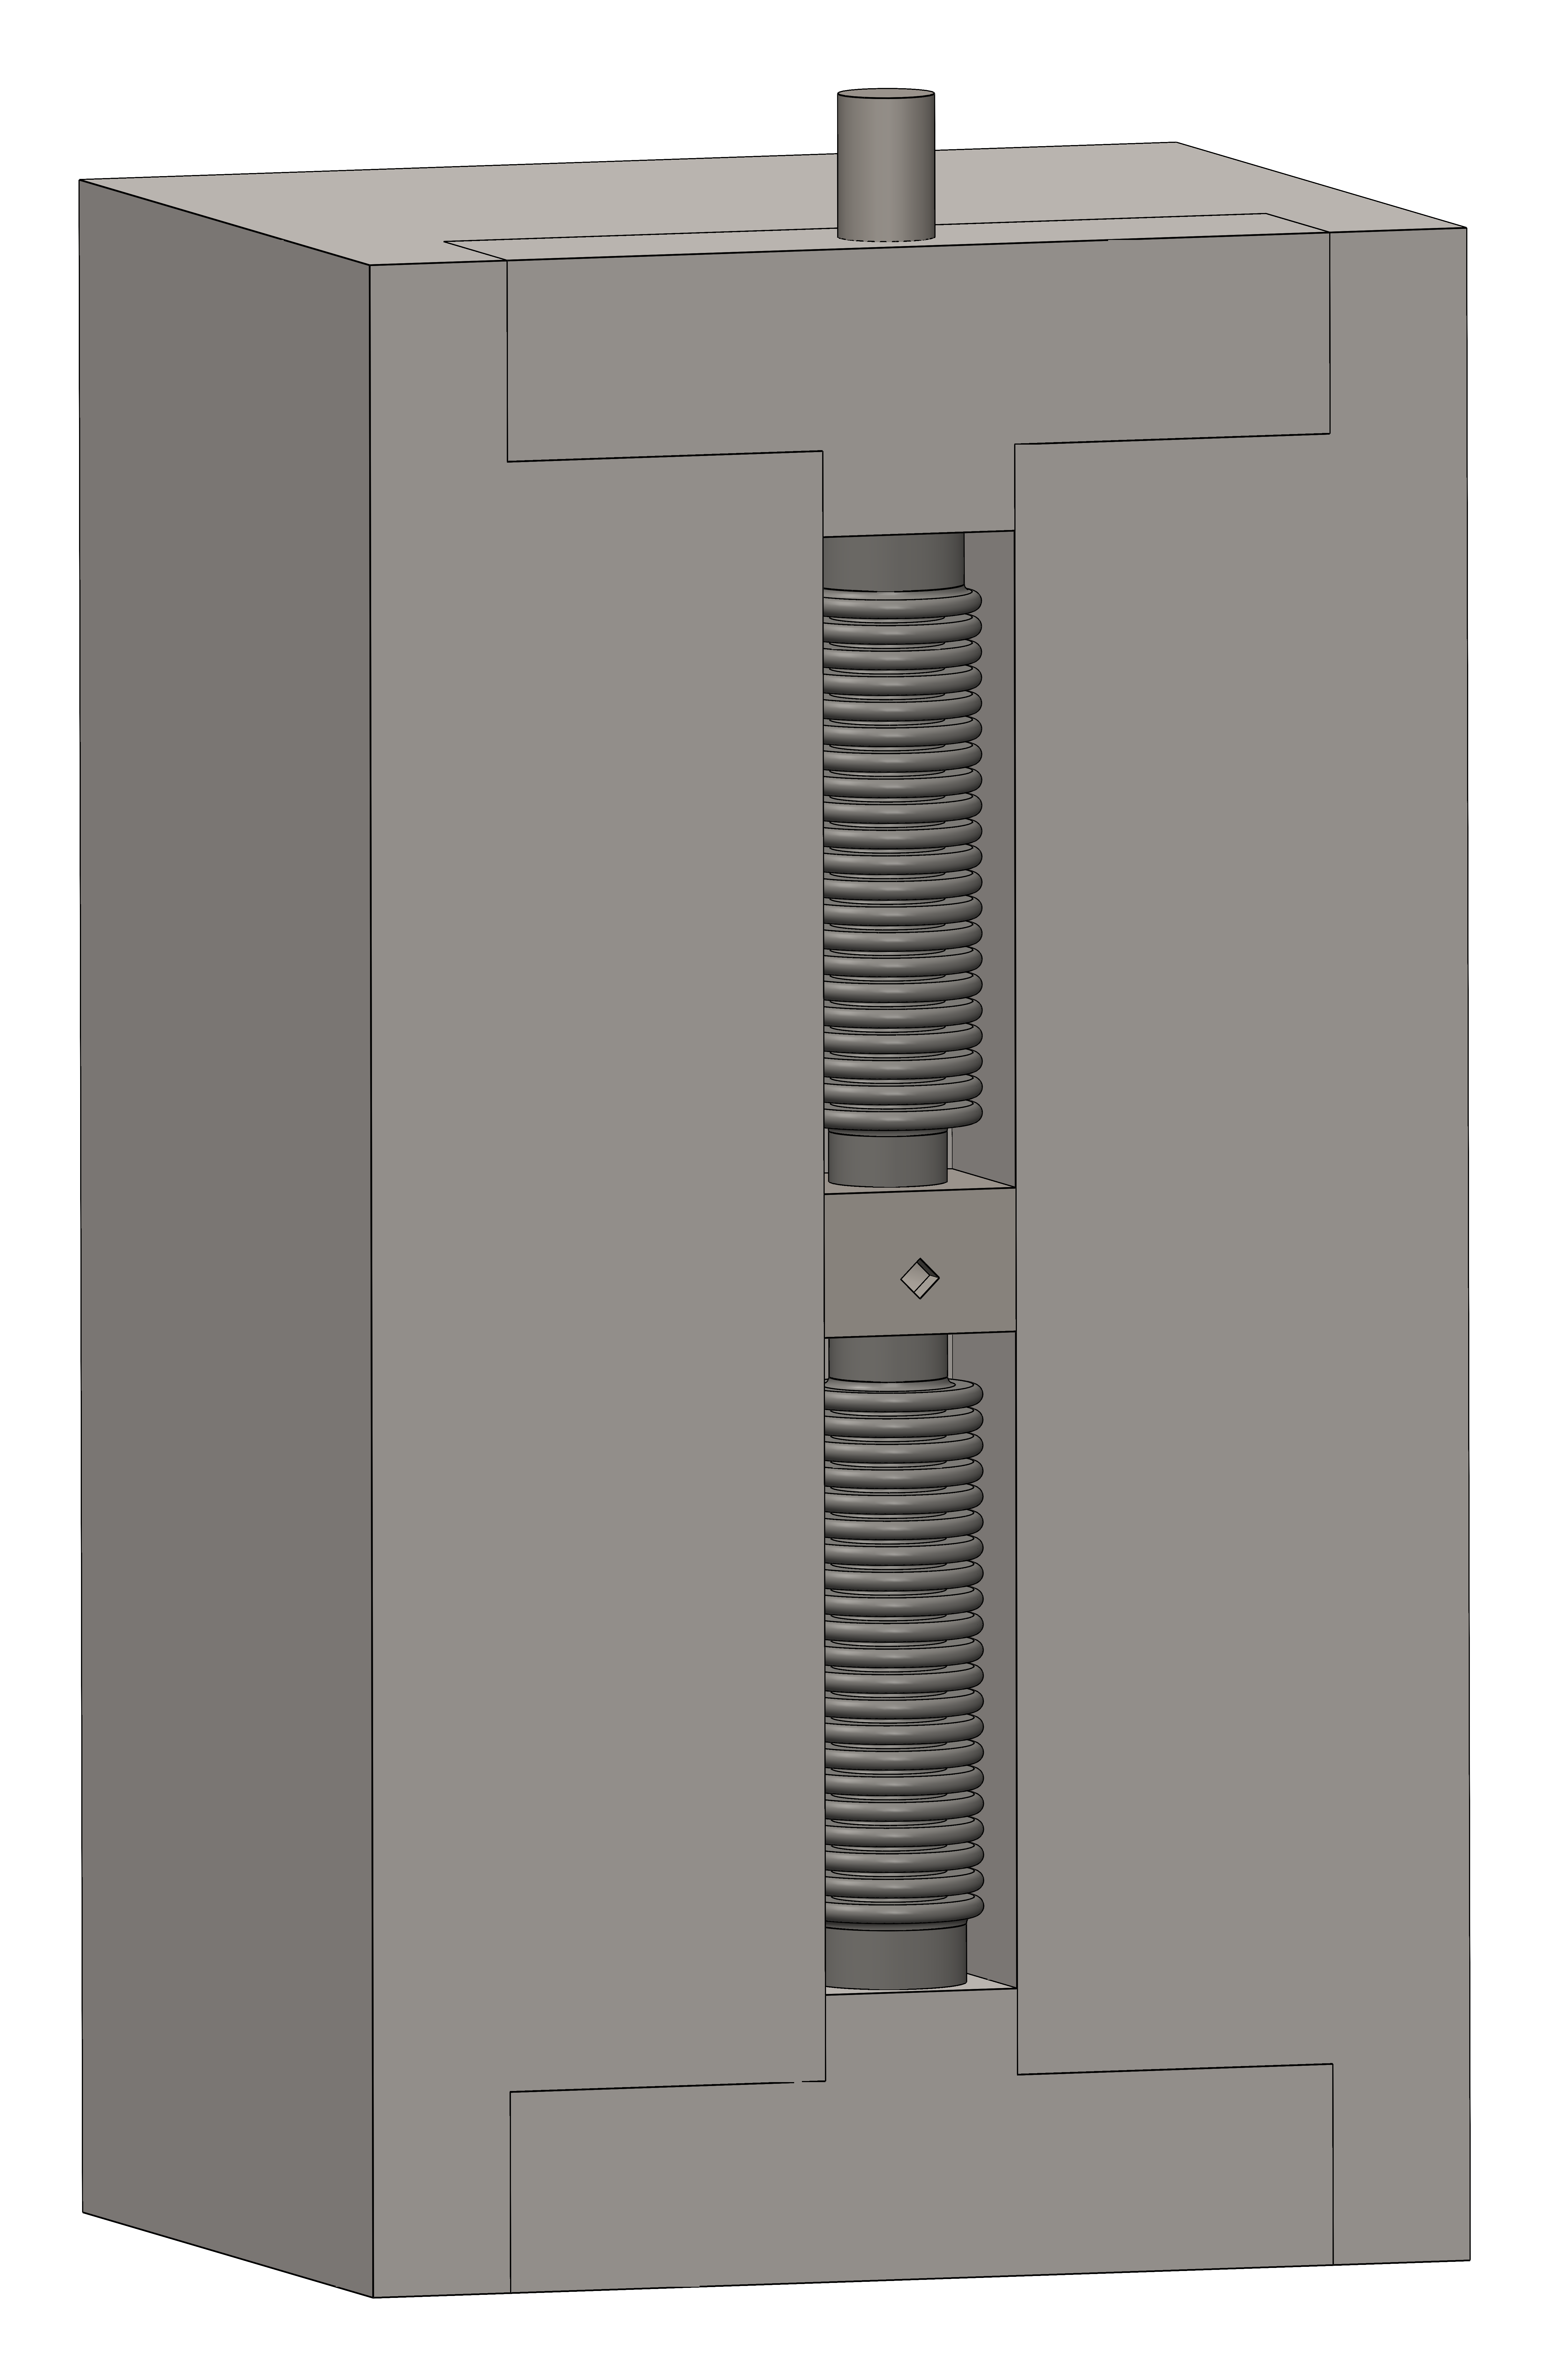
\includegraphics[height=3in]{V1_bellows_qual.png}
				\caption{Housing Center and bellows}
				\label{fig:V1_bellows}
				\end{minipage}
			\end{figure}

			\vspace{-1em}
			\begin{figure}[H]
					\centering
					\begin{subfigure}{0.45\textwidth}
							\centering
							% 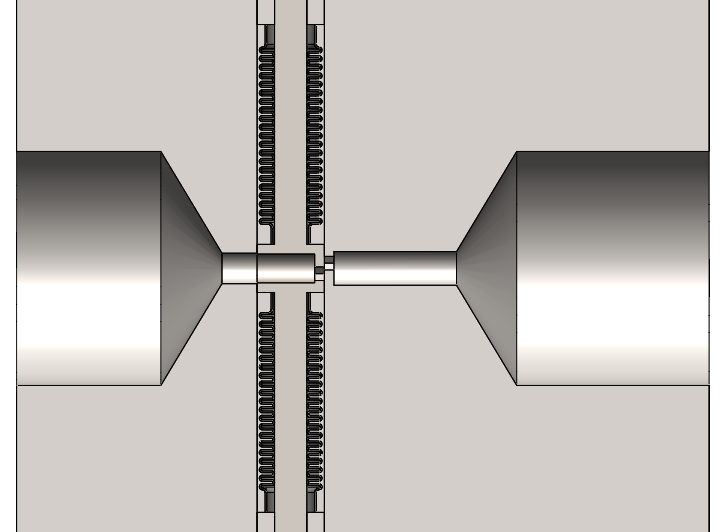
\includegraphics[width=\textwidth]{cut_zoom.png}
							\includegraphics[width=\textwidth]{cut_zoom_qual.png}
							\caption{Valve subsystem, section view}
							\label{fig:cut_zoom}
					\end{subfigure}
					\hfill
					\begin{subfigure}{0.39\textwidth}
							\centering
							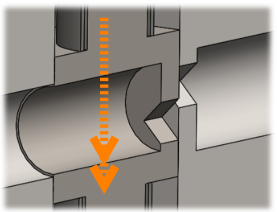
\includegraphics[width=\textwidth]{cut_zoom_zoom_crop.png}
							\caption{Valve, section view (detail)}
							\label{fig:cut_zoom_zoom_crop}
					\end{subfigure}
					\caption{Section views}
					\label{fig:cut_zooms}
			\end{figure}

		\subsection{Actuator Subsystem}
		\label{subsec:design:overview:act}

			The actuator subsystem (Figures~\ref{fig:act_full}, \ref{fig:act_exploded}, \ref{fig:act_ID}) sits atop the valve housing, where it maintains equilibrium with the surrounding ambient air temperature.
			It comprises an internal expansion rod to drive the valve stem, an external mount to suspend it from above, a screw and washer to secure them together, and a belleville washer to enable precise calibration.

			\begin{figure}[H]
				\centering
				\begin{minipage}{.4\textwidth}
					\centering
					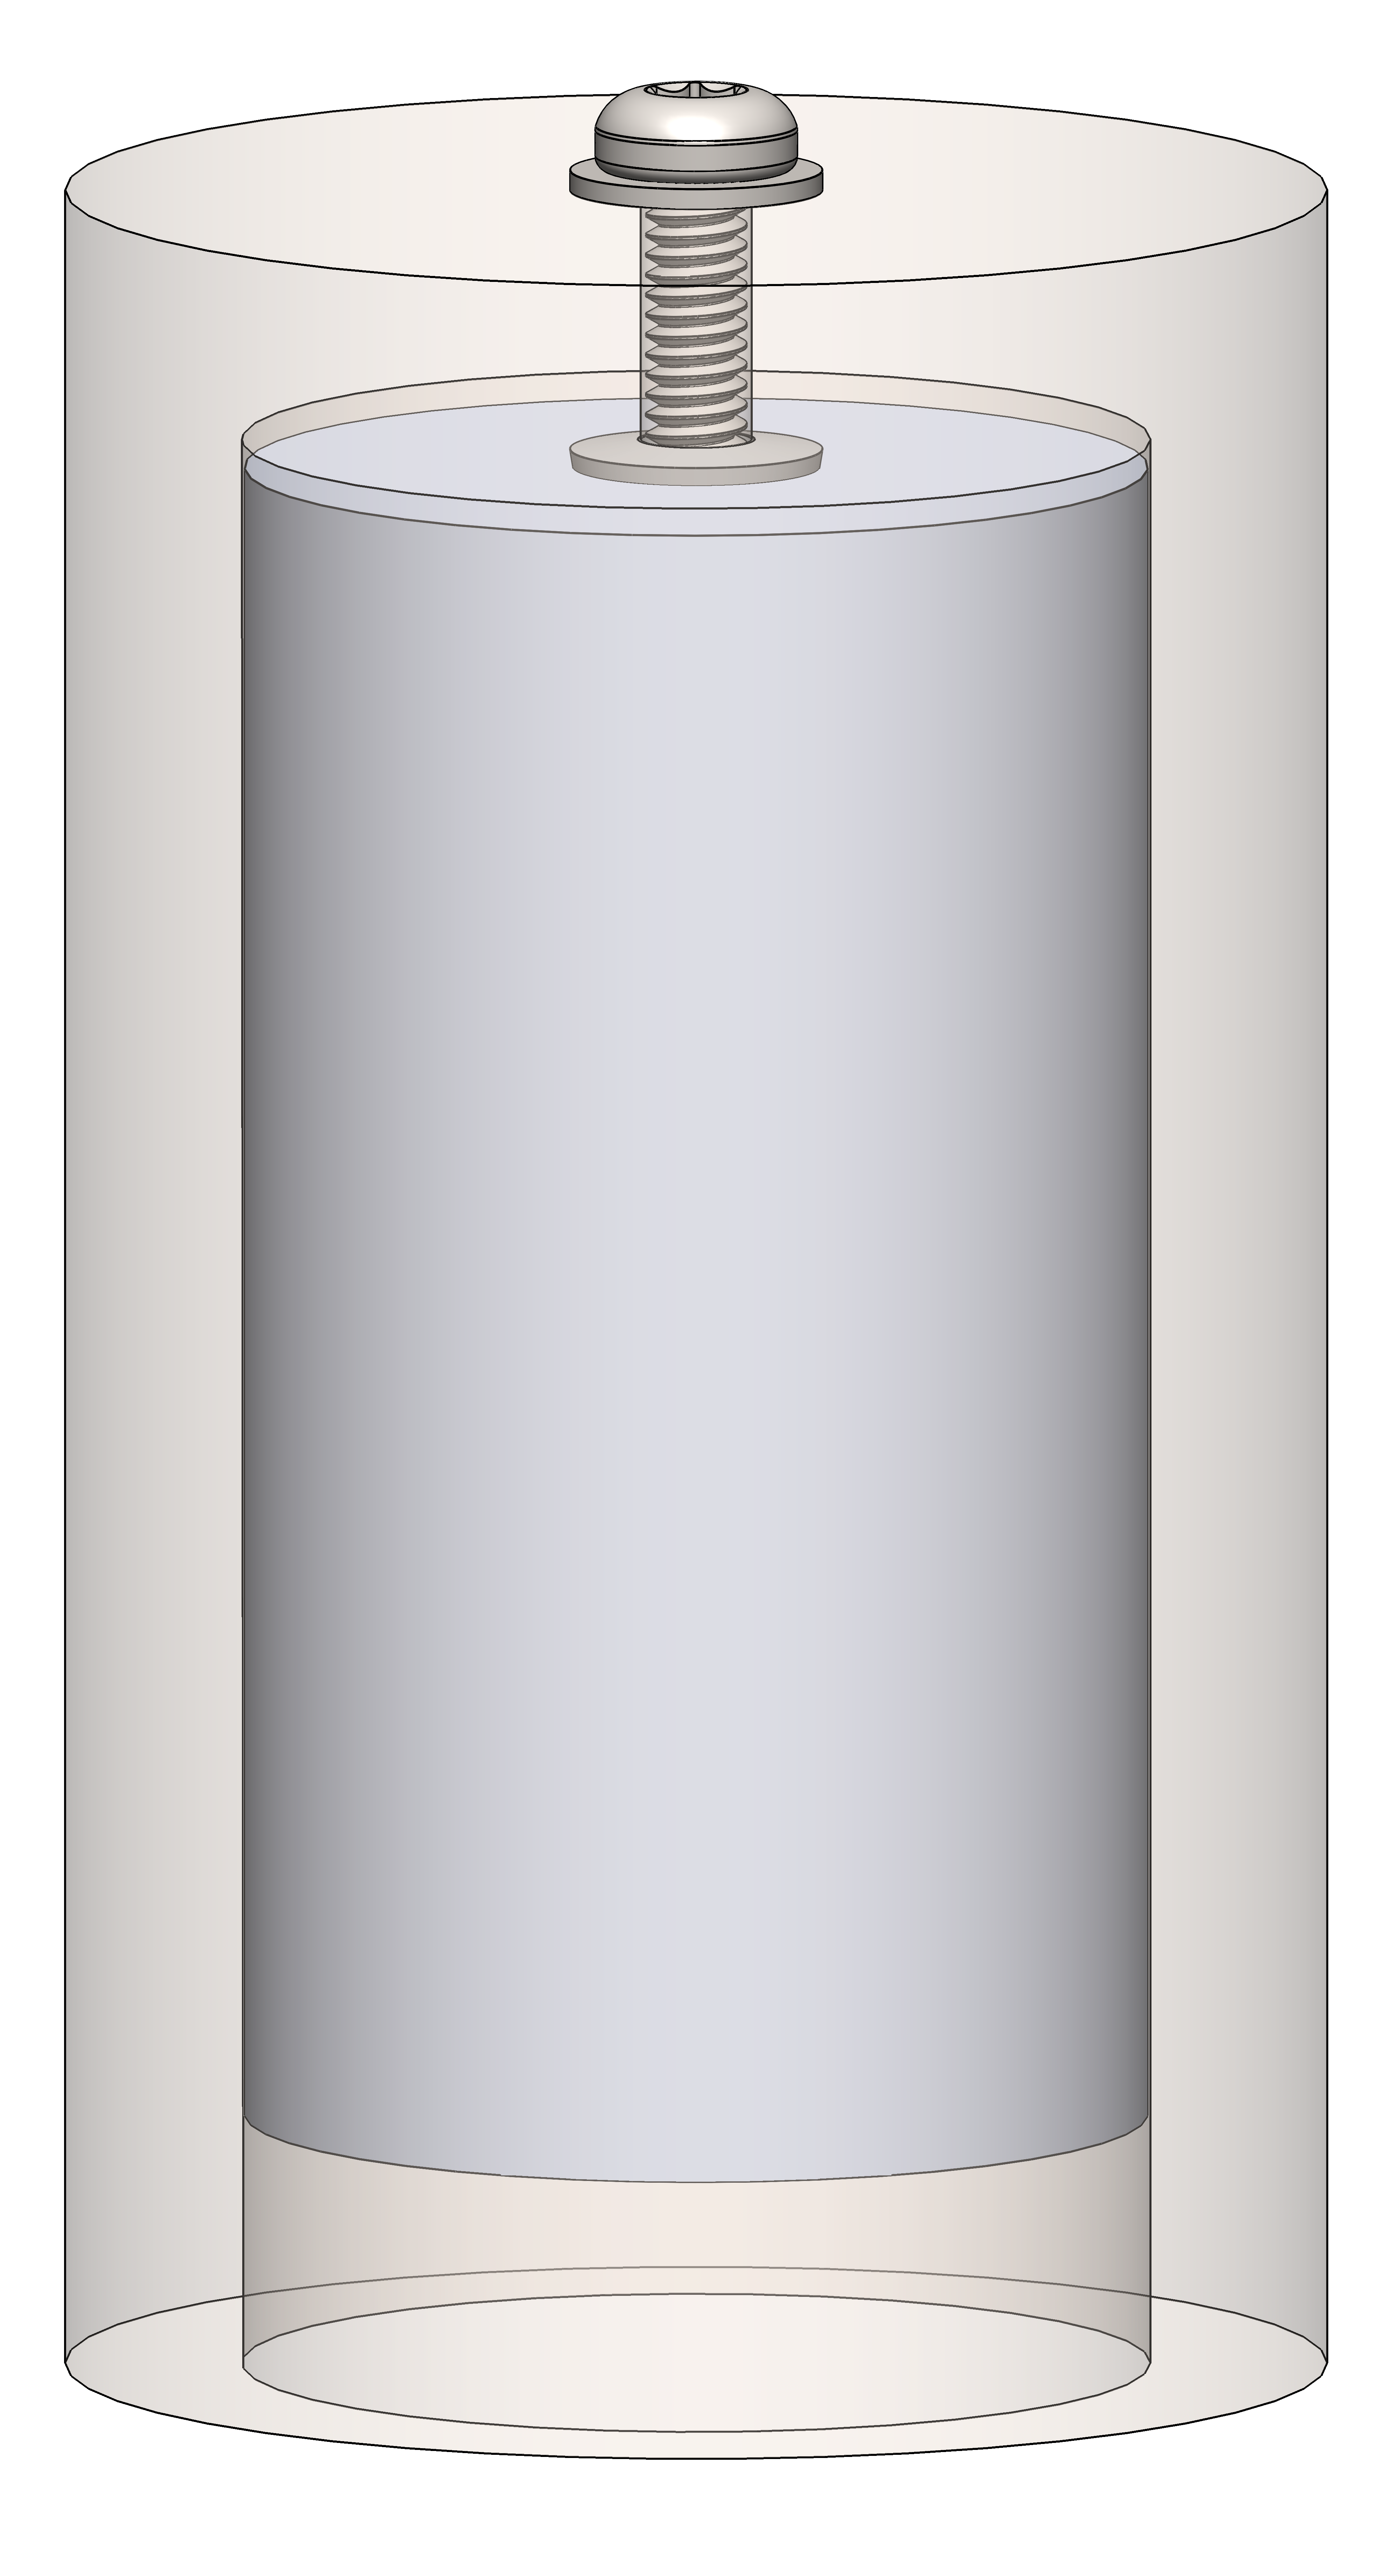
\includegraphics[height=.3\textheight, width=\textwidth, keepaspectratio]{Act_full_qual.png}
					\caption{Actuator subsystem}
					\label{fig:act_full}
				\end{minipage}
				\hfill
				\begin{minipage}{.29\textwidth}
					\centering
					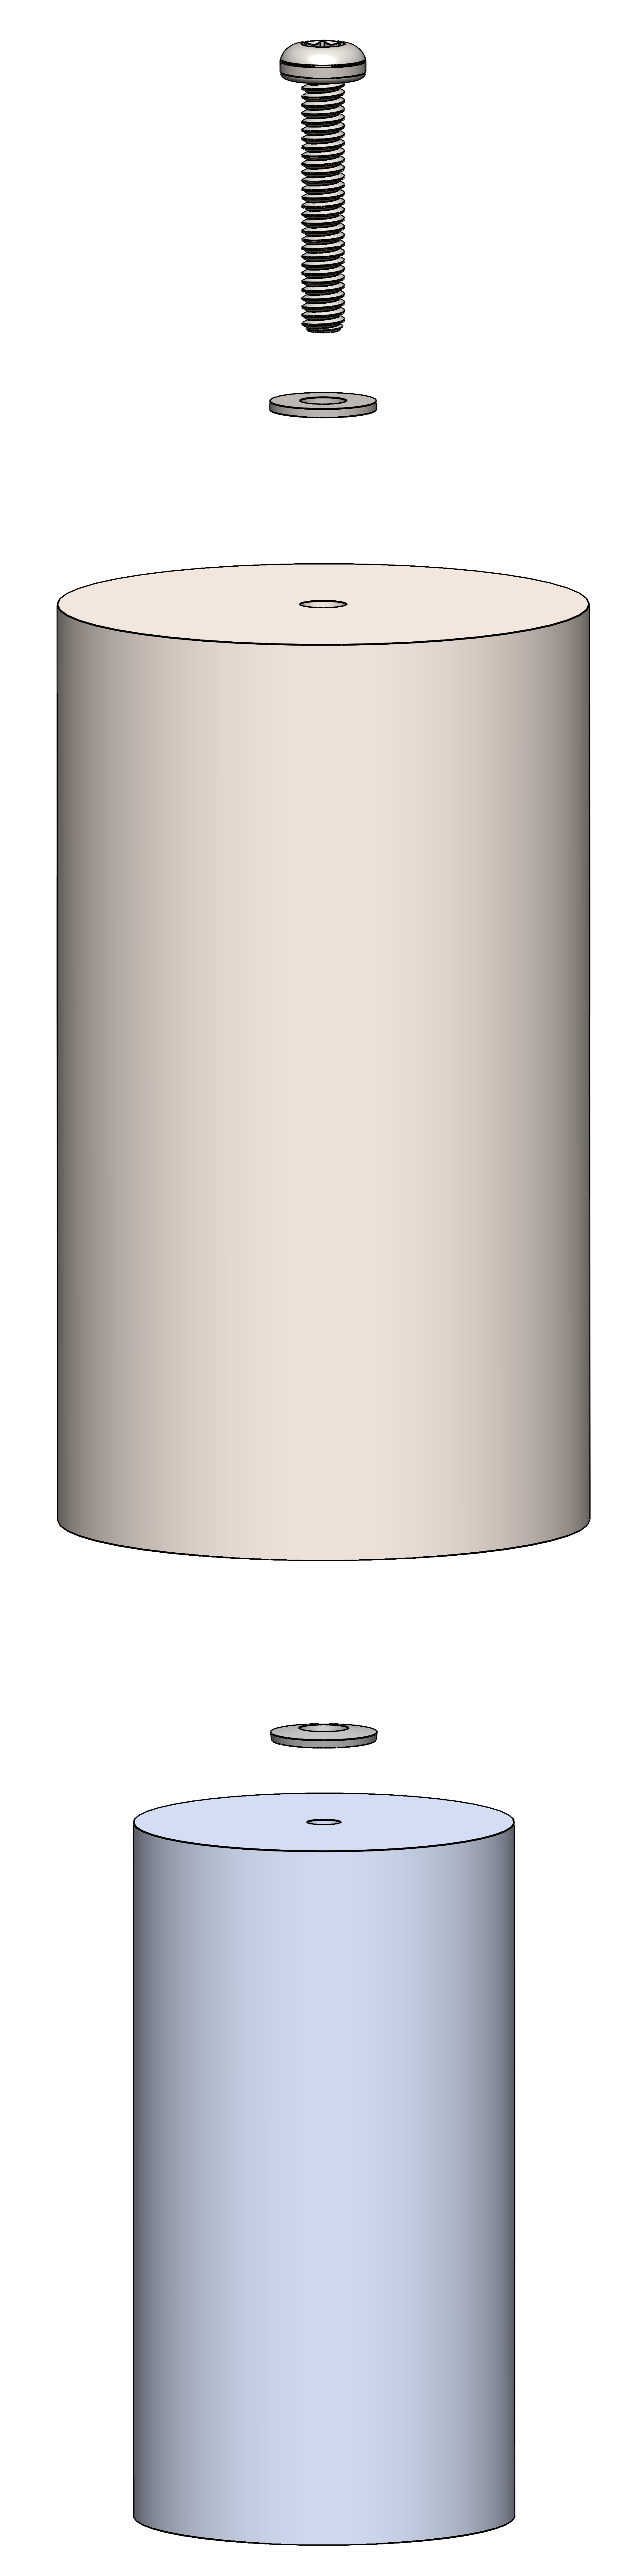
\includegraphics[height=.3\textheight, width=\textwidth, keepaspectratio]{Act_exploded_qual.png}
					\caption{Actuator subsystem exploded view}
					\label{fig:act_exploded}
				\end{minipage}
				\hfill
				\begin{minipage}{.29\textwidth}
					\centering
					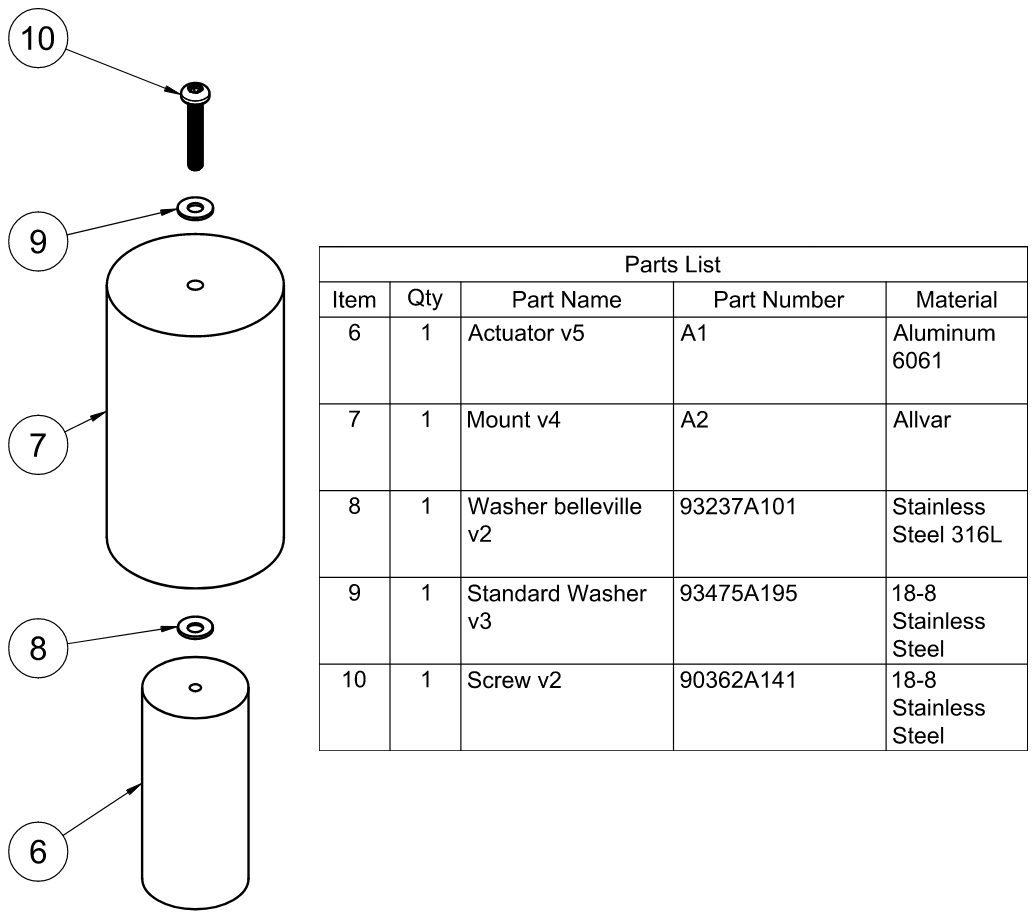
\includegraphics[height=.3\textheight, width=\textwidth, keepaspectratio]{Act_ID.png}
					\caption{Actuator subsystem part identification}
					\label{fig:act_ID}
				\end{minipage}
			\end{figure}


			The central aluminum expansion rod (6, aka the ``actuator''\footnote{
				Note that the actuator (A1 in the drawings in Appendix~\ref{app:drawings}) would best be named distinctly from its corresponding subsystem.
				This is a legacy convention from earlier stages in the design process when the mount was a distinct subsystem.
			}) nests inside an ALLVAR mount (7), suspended by the screw-washer assembly (8, 9, 10).
			The base of the mount is electron beam welded to the top of the valve housing.
			The assembly is centered about the valve stem, which protrudes through the housing and is welded to the base of the expansion rod.
			This connection is shown in Figure~\ref{fig:Act_cut}.

			\begin{figure}[h]
					\begin{minipage}[b]{1.5748in}
							\centering
							\includegraphics[width=1.5748in]{act_size.png}	% DO NOT CHANGE WIDTH; USED FOR ACTUAL SIZE
							\captionof{figure}{\device\ actual size}
							\label{fig:act_size}
					\end{minipage}
					\hfill
					\begin{minipage}[b]{0.72\textwidth}
							\centering
							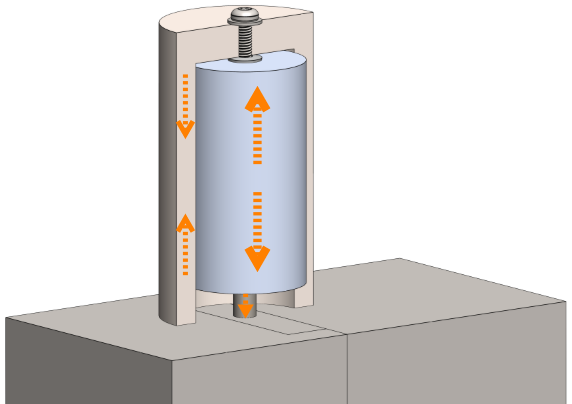
\includegraphics[width=\textwidth]{Act_cut_qual.png}
							\captionof{figure}{\device\ full assembly}
							\label{fig:Act_cut}
					\end{minipage}
			\end{figure}

			Figure~\ref{fig:act_size} shows the actual size of the \device\ when printed on $8 \nicefrac{1}{2}'' \times 11''$ paper.

			The actuator drives the valve stem motion.
			Aluminum's coefficient of thermal expansion (CTE) is significantly higher than that of Invar 36, causing the expansion rod to expand relative to the rest of the assembly when heated.
			ALLVAR, a proprietary alloy manufactured by ALLVAR Alloys, shrinks when heated even faster than the aluminum expands.
			Because the actuator is mounted from the top, this bimetallic actuator produces more compound displacement than either metal would on its own.
			As the ambient temperature rises, the ALLVAR mount shrinks, lowering the expansion rod from above;
			this, in turn, expands downwards, driving the valve stem and closing the orifice.
			As the temperature decreases, the components reverse direction:
			the mount expands, lifting the expansion rod, which shrinks and lifts the valve stem to open the orifice.

			The expansion rod is thermally separated from the internal gas by a \SI{5}{\milli\meter} gap. Heat transfer must be minimized from this gas, which will be up to \SI{20}{\degreeCelsius} hotter than the outside air.
			Some heat will still transfer, altering the perceived ambient temperature and introducing error into the system,
			but the thick housing wall, minimal contact between subsystems, and continual free convection with the atmosphere will minimize this error.

			Small machining and assembly errors may introduce a constant offset. For instance, if the valve stem is over-dimensioned by \SI{10}{\micro\meter},
			the orifice height will be \SI{10}{\micro\meter} too high at all times, adding a constant \SI{8}{\micro\meter} to the effective diameter\footnote{as calculated in Appendix~\ref{app:calcs:orifice_geometry}}.
			Even this deviation is significant relative to its \SIrange{10}{20}{\micro\meter} tolerance window,
			illustrating the necessity to minimize independent components.
			To counter this potential constant error, the actuator subsystem includes a calibration stack.
			As the assemblers tighten the screw, fastening the expansion rod inside the mount,
			the belleville washer between them compresses. This maintains consistent tension in the screw as the relative positions of the two cylinders are tuned.

			The complete Bill of Materials and Engineering Drawings for the \device\ can be found in Appendix~\ref{app:BOM} and \ref{app:drawings}, respectively.
			Table~\ref{tab:part_num} summarizes the part numbers for each component of the \device, which will be used for reference in the following sections.

			\begin{table}[H]
				\centering
				\caption{Component part numbers}
				\label{tab:part_num}
				\renewcommand{\arraystretch}{1.3}
				\begin{tabular}{
					>{\centering\arraybackslash}p{0.08\textwidth}
					>{\raggedright\arraybackslash}p{0.22\textwidth}
					>{\centering\arraybackslash}p{0.18\textwidth}
					>{\raggedright\arraybackslash}p{0.22\textwidth}
				}
				\toprule
				\textbf{Item} & \textbf{Part Name} & \textbf{Part Number} & \textbf{Material} \\
				\midrule
				\multicolumn{4}{l}{\textit{Valve Sub-Assembly (V0)}} \\
				\midrule
				1 & Housing Inlet  & V2              & Invar 36     \\
				2 & Housing Center & V1              & Invar 36     \\
				3 & Housing Outlet & V3              & Invar 36     \\
				4 & Valve Orifice  & V4              & Invar 36     \\
				5 & Bellows        & I718-159-72-430 & Inconel 718  \\
				\midrule
				\multicolumn{4}{l}{\textit{Actuator Sub-Assembly (A0)}} \\
				\midrule
				6  & Actuator          & A1        & 6061 Aluminum        \\
				7  & Mount             & A2        & ALLVAR 30            \\
				8  & Belleville Washer & 93237A101 & Stainless Steel 316L \\
				9  & Standard Washer   & 93475A195 & 18-8 Stainless Steel \\
				10 & Screw             & 90362A141 & 18-8 Stainless Steel \\
				\bottomrule
				\end{tabular}
			\end{table}

	\section{Design Justification}
	\label{sec:design:just}

		\subsection{Transfer Functions and Critical Dimensions}
		\label{subsec:design:just:TF}

			Specifications \specref{V.1.1} and \specref{A.1.1} require specific input-output relationships to satisfy system requirement \specref{R.1}, the Required Relationship:

			\RRfull

			These values are driven by the geometry described above and by the dimensions we select for each part.

			\newpage%
			\begin{multicols}{2}
				\begin{figure}[H]
						\centering
						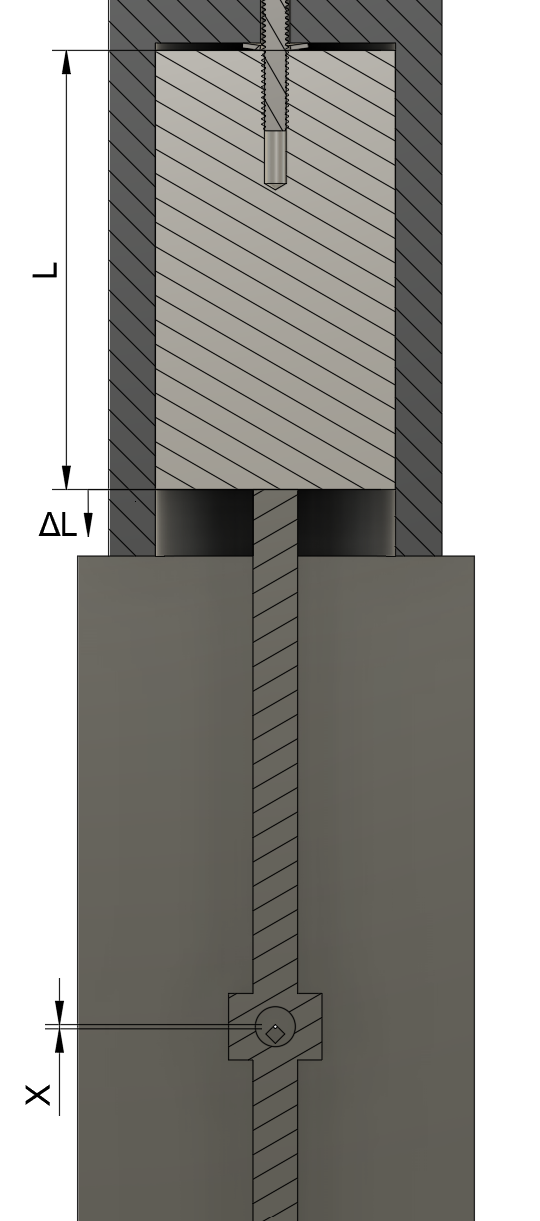
\includegraphics[height=.6\textheight]{L_X.png}
						\caption{Dimension definitions}
						\label{fig:L_X}
				\end{figure}
			\newcolumn
				Let us define the change in the actuator length, $\Delta L$, as the vertical extension of the aluminum expansion rod, which includes any rigid-body motion driven by the mount.
				See Figure~\ref{fig:L_X}. Thus, if the mount shrinks, and the expansion rod grows, by \SI{1}{\micro\meter} each, the length $L$ will increase by \SI{2}{\micro\meter}.
				This drives the valve stem an equal amount, lowering the valve stem and shrinking the orifice height $X$ by \SI{2}{\micro\meter}.

			\subsubsection{Valve Transfer Function}
			\label{subsubsec:design:just:TF:valve}

				The valve orifice geometry governs the transfer function

				\begin{equation*}
					\hat{G}_{V_0} = \frac{dD}{dL} = \frac{dD}{dX} \frac{dX}{dL}
				\end{equation*}

				that translates the change in the actuator's length, $L$\footnote{
					Note that the actuator movement may more readily be defined as the distance between the base of the mount and the base of the actuator, which in fact decreases as $L$ increases.
					The actuator length is also a legacy parameter from when the design featured a rigid Invar mount and only the expansion rod moved.},
				to a change in the effective diameter $D$.
				The orifice diameter is most readily defined by the vertical distance $X$ between its upper and lower vertices.
				As derived in Appendix~\ref{app:calcs:orifice_geometry}, the effective diameter of this orifice scales with the height by a constant factor such that

				\begin{equation}
					D_{eff} = \sqrt{\frac{2}{\pi}} X
				\end{equation}

				therefore

				\begin{equation}
					\frac{dD}{dX} = \sqrt{\frac{2}{\pi}}
				\end{equation}

				\end{multicols}

				The orifice shrinks as the actuator expands, yielding the second control derivative

				\begin{equation}
					\frac{dX}{dL} = -1
				\end{equation}

				Therefore, multiplying these together, we find

				\begin{equation}
					\hat{G}_{V_0} = -\sqrt{\frac{2}{\pi}} = \GV
				\end{equation}

				as prescribed.

				The valve subsystem also controls the reference orifice diameter $D_{ref}$.
				We can find this by calculating the orifice height at $T_{ref}$.
				According to dimensions from the engineering drawings in Appendix~\ref{app:drawings}, the top corner of the leading orifice lies

				\begin{equation*}
					\SI{40.201}{\milli\meter} - \SI{5}{\milli\meter} = \SI{35.201}{\milli\meter}
				\end{equation*}

				below the top surface of the housing, including a \SI{5}{\milli\meter} gap between that and the valve stem-actuator interface at this temperature.
				The bottom corner of the trailing orifice lies $\SI{35.519}{\milli\meter}$ below the same surface, resulting in an effective diameter of

				\begin{equation}
					D_{ref} = \sqrt{\frac{2}{\pi}} X_{ref} = \sqrt{\frac{2}{\pi}} (\SI{35.519}{\milli\meter} - \SI{35.201}{\milli\meter}) = \AzeroExact
					\label{eq:Dref}
				\end{equation}

				as specified.

			\subsubsection{Actuator Transfer Function}
			\label{subsubsec:design:just:TF:act}

			The bimetallic actuator expands at a constant rate with temperature, governing the transfer function
			
			\begin{equation*}
				\hat{G}_{A_0} = \frac{dL}{dT}
			\end{equation*}
			
			that translates the ambient temperature into motion.
			The length of each of its components drives that expansion rate. Its dimensions are shown in greater detail in Figure~\ref{fig:act_dim}.
			A belleville washer is compressed between the upper interior of the mount and the top surface of the actuator, held in place by the screw. Uncompressed, it measures \SI{0.6}{\milli\meter} tall;
			we will assume a compressed height of \SI{0.55}{\milli\meter}\footnote{
				The exact compression height of the belleville washer is, by nature, an unknown and varies between each device.
				Deviations will be accounted for in Chapter~\ref{chap:DFMEA}.}.
			A \SI{5}{\milli\meter} gap, spanned by the valve stem, separates the free end of the actuator from the housing, thermally insulating the actuator from direct heat transfer with the hot internal gas.

			\begin{wrapfigure}{l}{0.49\textwidth}
				\centering
				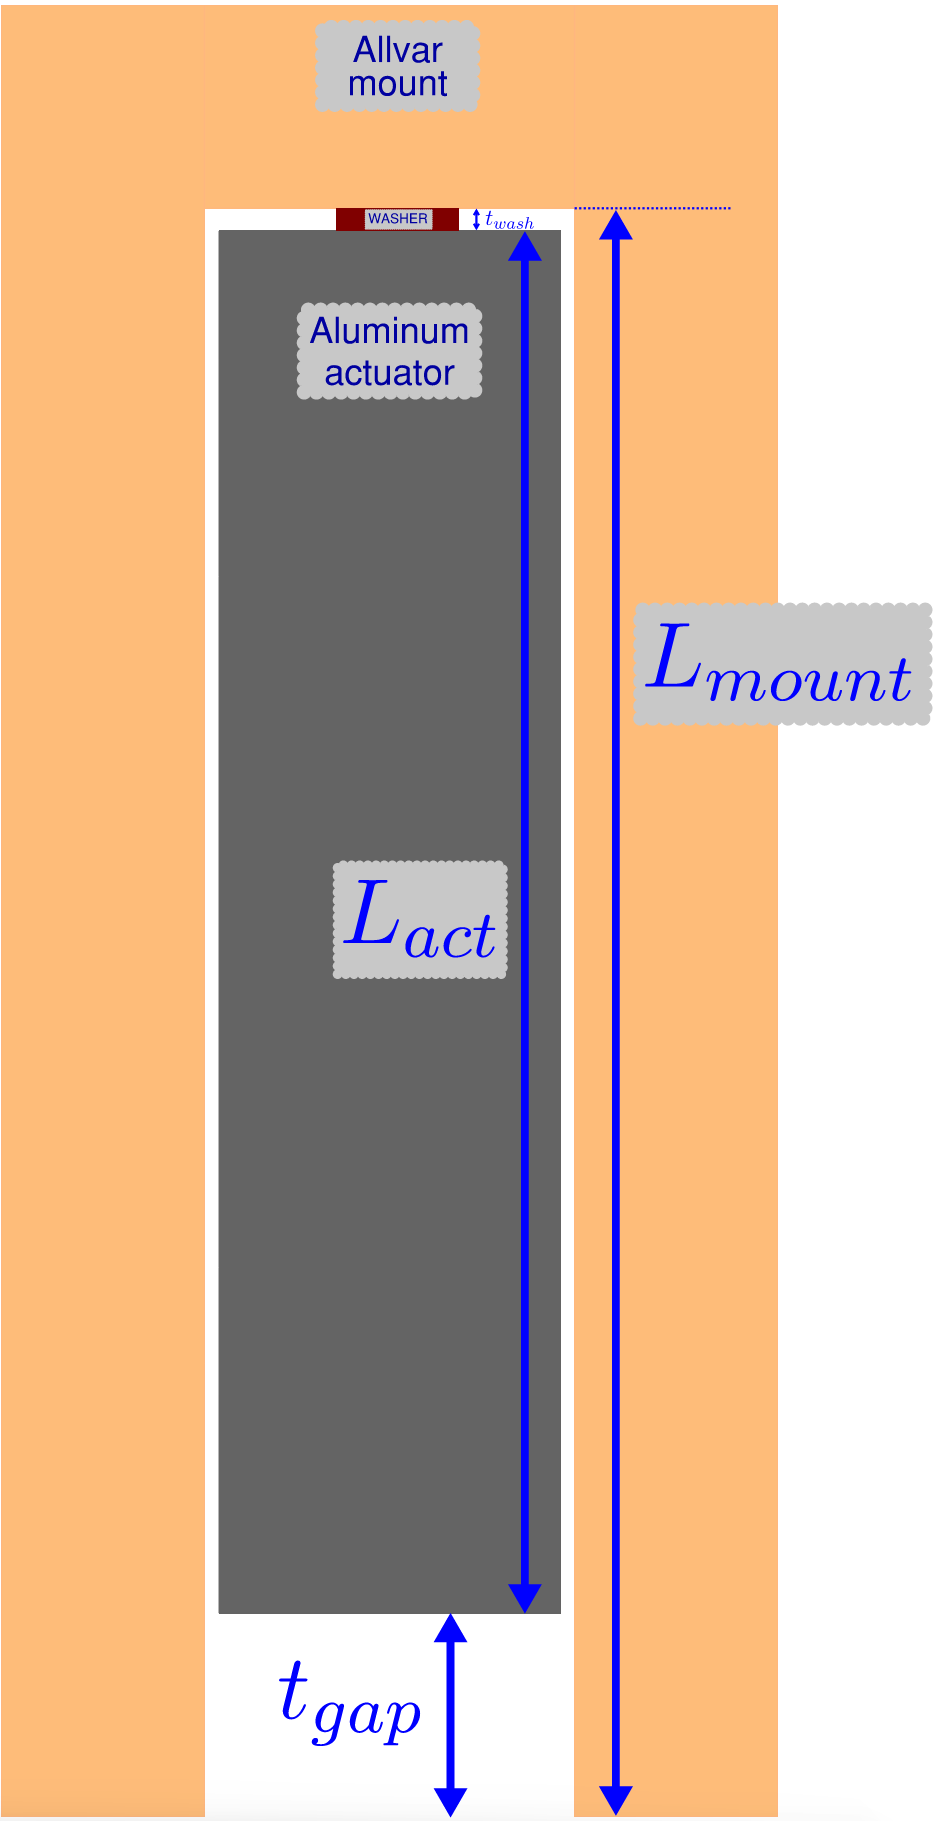
\includegraphics[width=0.47\textwidth]{Act_dim.png}
				\caption{Actuator dimension labels}
				\label{fig:act_dim}
			\end{wrapfigure}

			Assuming the base of the mount, welded to the housing, to be fixed,
			and assuming for now that the CTE of ALLVAR is positive,
			the expansion rod (aka the ``actuator'') will expand downwards as it is lifted upwards when heated. This action yields the actuation-temperature relationship in Equation~\eqref{eq:actuation}.
			Because ALLVAR's CTE is negative, the mount will shrink as the actuator expands, aiding its action. Thus, $L_{mount} \alpha_{mount}$ increases the actuation distance $\Delta L$ by a double-negative.
			Adding the dimensions in Figure~\ref{fig:act_dim} yields the geometric relations in Equation~\eqref{eq:act_dim}, giving us the following system of two equations:
			
			\begin{align}
				\Delta L = \left( L_{act} \alpha_{act} - L_{mount} \alpha_{mount} \right) \Delta T \label{eq:actuation}\\
				L_{mount} = t_{wash} + L_{act} + L_{gap} \label{eq:act_dim}
			\end{align}

			The target, from Specification \specref{A.1.1}, is

			\begin{equation}
				\frac{dL}{dT} = \frac{\Delta L}{\Delta T} = \GA
			\end{equation}

			Plugging in the following values (material properties are from Appendix~\ref{app:datasheets:mat}):

			\begin{align*}
				\alpha_{act} &= \specActuatorCTE \\
				\alpha_{mount} &= \specMountCTE \\
				t_{wash} &= \SI{0.55}{\milli\meter} \\
				L_{gap} &= \SI{5}{\milli\meter}
			\end{align*}

			we obtain the following results:

			\begin{align}
				L_{act} &= \frac{\frac{\Delta L}{\Delta T} + (t_{wash} + L_{gap}) \alpha_{mount}}{\alpha_{act} - \alpha_{mount}} \notag \\[12pt]
				&= \frac{\GA + (\SI{5.55}{\milli\meter}) \cdot (\specMountCTE)}{\specActuatorCTE - \specMountCTE} = \specOrigActuatorLength \label{eq:L_act}\\[12pt]
				L_{mount} &= L_{act} + t_{wash} + L_{gap} = \SI{38.541}{\milli\meter} \label{eq:L_mount}
			\end{align}

			These critical dimensions ensure that the actuator subsystem maintains the specified output

			\begin{equation}
				\hat{G}_{A_0} = \frac{A_1}{-\sqrt{\frac{2}{\pi}}} = \GA
			\end{equation}

			Altogether, $\hat{G}_{V_0},\ \hat{G}_{A_0}, \text{ and } D_{ref}$ combine to satisfy the functional system requirement \specref{R.1}:
			
			\begin{equation}
				\begin{aligned}
					D_{eff} &= \hat{G}_{V_0} \hat{G}_{A_0} \Delta T + D_{ref} \\
					&= \left( \GV \right) \left( \GA \right) \Delta T + \AzeroExact \\
					&= \left( \AoneExact \right) \Delta T + \AzeroExact \\
					&= A_1 \Delta T + A_0
				\end{aligned}
			\end{equation}

				This bimetallic architecture enables the actuator to be half the length of solitary high-expansion metal, keeping its total length (\SI{45.55}{\milli\meter}, accounting for the mount's upper wall and the screw that protrudes from its top) within the specified vertical mechanical envelope.

				It is useful to note that the total required motion of the actuator is

				\begin{equation}
					\Delta L = \frac{dL}{dD} \Delta D = \frac{\Delta D_{eff}}{\hat{G}_{V_0}} = \frac{D_{hot} - D_{cold}}{-\sqrt{\frac{2}{\pi}}} = \frac{\SI{170.2}{\micro\meter} - \SI{383.5}{\micro\meter}}{-\sqrt{\frac{2}{\pi}}} = \specActDefTotal
				\end{equation}

				an imperceptible motion to the human eye. The maximum deflection from the reference point is

				\begin{equation}
					\Delta L = \frac{D_{cold} - D_{ref}}{-\sqrt{\frac{2}{\pi}}} = \frac{\SI{383.5}{\micro\meter} - \SI{254.0}{\micro\meter}}{-\sqrt{\frac{2}{\pi}}} = \specActDefHot
					\label{eq:act_def_hot}
				\end{equation}

				These values will be used elsewhere to calculate conditions at the extrema.

		\subsection{Valve Architecture Selection Criteria}
		\label{subsec:design:just:geo_sel}

			To the first-time observer, the valve geometry appears peculiar and unintuitive.
			The diamond-orifice architecture was developed after serious consideration and several design iterations, described in more detail in Appendix~\ref{app:PM}.
			The following selection criteria motivated the final design of the valve orifice:

			\begin{itemize}
				\item Linearity
				\item Simplicity
				\item Direct Actuation
			\end{itemize}

			The Required Relationship stipulates that the \device\ maintain a constant temperature-diameter conversion rate, represented by the joint transfer function

			\begin{equation*}
				\hat{G}_{RR} = \hat{G}_{V_0} \hat{G}_{A_0} = A_1
			\end{equation*}

			in Section~\ref{subsec:intro:specs:RR}. $A_1$ is expressly first-order. Any nonlinear behavior in one subsystem must be either reparameterized\footnote{i.e. corrected.} in the other subsystem, an imprecise process involving a complex mechanical interface, or tolerated as error.
			$\hat{G}_{RR}$'s tolerable error is limited to 5\% of $A_1$, or \SI{76.2}{\nano\meter\per\celsius}, a razor-thin margin.
			To best reach this target, the selection process only permitted subsystem architectures that exhibit first-order behavior with minimal degrees of freedom and a direct subsystem interface.
			
			Many actuator design alternatives readily fit these criteria, as most materials maintain a linear thermal expansion rate.
			However, most valve architectures more readily translate their driving motion directly to the area of their orifice rather than its effective diameter.
			For instance, the needle valve, a reliable and precise design commonly used for gas flow control, subtracts one circle (the cross-section of its needle) from another (the hole the needle is inserted into).
			This difference causes a constant change in orifice area as the needle is moved.
			Because

			\begin{equation*}
				A \propto D_{eff}^2
			\end{equation*}

			as established in Appendix~\ref{app:calcs:orifice_geometry}, the effective diameter follows a second-order output.
			A linear relationship requires a regular orifice geometry (such as a circle, a square, or a hexagon) that maintains its shape, all sides changing at the same rate.
			Many flexible membranes required to construct a circular orifice permit hydrogen embrittlement and diffusion, disqualifying a circular geometry.
			Complex-polygon architectures, such as hexagonal camera-style aperture, comprise more degrees of freedom than the precise relationship allows.
			The diamond orifice, on the other hand, performs linearly with two interfacing components and a single degree of freedom.
			Although it was an entirely novel approach to this problem, the design fit all three selection criteria and, as demonstrated in Chapter~\ref{chap:DFMEA}, ultimately satisfies the Required Relationship.

		\subsection{Pressure Capacity}
		\label{subsec:design:just:P}

			The Invar housing, consisting of the Housing Inlet, Outlet, and two Centers, is designed and assembled to withstand \specPressure\ internal pressure without yielding according to Specification \specref{V.3.1}. 
			The Inlet and Outlet have threaded cylindrical internal geometries.
			The central cavity, which houses the internal valve components, forms a rectangular prism, all of whose sides are wetted at pressure.

			To determine the appropriate wall thickness required to sustain the internal pressure in the inlet and outlet sections, the housing is modeled as a thick-walled cylinder.
			The thickness $t$ of the housing is defined as the shortest distance from the inner wall to the outer wall.
			The following equations are used to verify structural integrity under the specified conditions.
			Since internal pressure constitutes the only significant structural load, external forces on the housing are neglected.

			\begin{table}[H]
				\centering
				\caption{Valve housing parameter values}
				\label{tab:housing_parameters}
				\begin{tabularx}{\textwidth}{l X l}
					\toprule
					\textbf{Parameter} & \textbf{Description} & \textbf{Value} \\
					\midrule
					Material &
					&
					Invar 36
					\\\addlinespace
					$r_i$ &
					Inner radius &
					\SI{12.194}{\milli\meter}
					\\\addlinespace
					$t$ &
					Wall thickness (minimum) &
					\SI{7.806}{\milli\meter}
					\\\addlinespace
					$r_o$ &
					Outer radius (minimum) &
					\SI{20}{\milli\meter}
					\\\addlinespace
					$P$ &
					Internal pressure &
					$\specPressure$
					\\\addlinespace
					$S_y$ &
					Yield strength &
					\SI{276}{\mega\pascal}
					\\\bottomrule
				\end{tabularx}
			\end{table}

			The principal stresses, those along the three orthogonal axes, are as follows\cite{ref_shigley}:
			\begin{equation}
			\sigma_{\theta} = P \left( \frac{r_o^2 + r_i^2}{r_o^2 - r_i^2} \right) = 68.95 \left( \frac{20^2 + 12.194^2}{20^2 - 12.194^2} \right) \approx \SI{150.54}{\mega\pascal} \quad (\text{Hoop Stress})
			\end{equation}

			\begin{equation}
			\sigma_{r} = -P \approx \SI{-68.95}{\mega\pascal} \quad (\text{Radial Stress})
			\end{equation}

			\begin{equation}
			\sigma_{z} = P \left( \frac{r_i^2}{r_o^2 - r_i^2} \right) = 68.95 \left( \frac{12.194^2}{20^2 - 12.194^2} \right) \approx \SI{40.80}{\mega\pascal} \quad (\text{Longitudinal Stress})
			\end{equation}
			
			The housing must be designed against yield, or plastic\footnote{Irreversible.} deformation.
			Its yield strength can be readily compared against the von Mises stress, which measures the distortion energy as a combination of the principal stresses.

			\begin{equation}
				\begin{aligned}
					\sigma_{\text{vm}} &= \sqrt{\frac{(\sigma_\theta - \sigma_r)^2 + (\sigma_r - \sigma_z)^2 + (\sigma_z - \sigma_\theta)^2}{2}} \\
					&= \sqrt{\frac{(150.54 - (-68.95))^2 + (-68.95 - 40.80)^2 + (40.80 - 150.54)^2}{2}}
				\end{aligned}
			\end{equation}

			\begin{equation}
			\approx \SI{190.08}{\mega\pascal}
			\end{equation}

			This yields a safety factor of

			\begin{equation}
			FS = \frac{S_y}{\sigma_{\text{vm}}} = \frac{276}{190.08} \approx 1.45 > 1
			\end{equation}

			verifying that the cylindrical Housing Inlet segment carries sufficient material to hold the maximum specified internal pressure.
			System pressure capacity drove the valve subsystem's lateral mechanical envelope of \SI{40}{\milli\meter},
			which is sufficiently thick to satisfy its pressure requirements and well within its size constraints.

			The above estimate is conservative and assumes a cylindrical exterior with a wall thickness equal to the thinnest dimension of the actual design.
			The rectangular housing exterior circumscribes this cylinder, providing extra strength.
			
			The housing center pieces are joined using welded connections and designed with a wall thickness of \SI{10}{\milli\meter}, which is greater than the minimum required thickness of \SI{7.806}{\milli\meter}, to ensure that the pressure boundary is maintained at the critical junction where the three sections of the housing meet.
			Because the center pieces form a rectangular prism, the stress distribution is more complex than in a cylindrical geometry, and was difficult to model analytically. However, the increased thickness of \SI{10}{\milli\meter} provides a significant safety margin to ensure that the housing center can withstand the internal pressure without failure.
			Flat-walled pressure vessel behavior and stress concentrations at the corners may, however, produce more than the critical stress;
			this risk is evaluated in more detail in Section~\ref{sec:comp_proto}.

		\newpage % Delete if necessary
		\subsection{Hermetic Seal}
		\label{subsec:design:just:bellows}

		\begin{wrapfigure}{l}{0.45\textwidth}
				\centering
				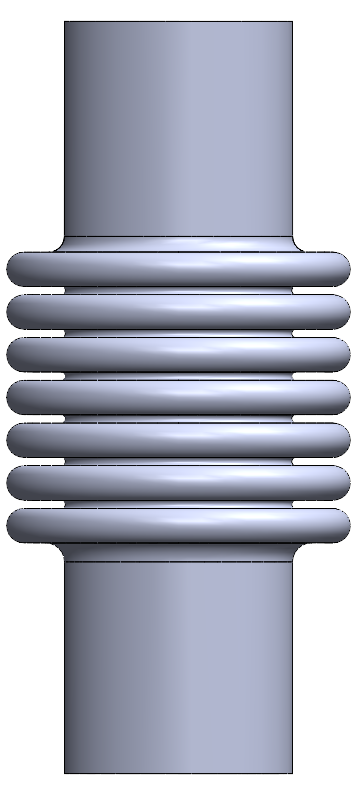
\includegraphics[width=0.35\textwidth]{bellows.png}
				\caption{I718-159-72-430 bellows}
				\label{fig:bellows}
		\end{wrapfigure}

		The \device\ requires mechanical penetration of a pressure vessel. Specifications \specref{V.3.2} and \specref{V.3.3} require a hermetic seal\footnote{
			Named after the Greek god Hermes\cite{ref_wilton_hermetic}, a hermetic seal limits gas leakage to nearly zero.
			It originates from the alchemical practice of fusing glass vessels together such that air cannot escape\cite{ref_gesner_1559}.
		} to prevent leakage through this interface.
		Typical polymer gaskets permit hydrogen diffusion and are subsequently embrittled, significantly limiting the lifetime of the seal.
		Hydrogen gas molecules, the smallest in existence, seep through the long polymer chain structures with ease, spurred by an enormous back pressure, and react with the polymer material.
		Flexible metal bellows bypass this concern with a hermetic seal that is directly fused between the valve stem and the housing structure.
		The flexible tube comprises convolutions that stretch and compress with little resistance when driven axially but can withstand substantial radial pressure loads.
		The I718-159-72-430, pictured in Figure~\ref{fig:bellows}, can hold a seal at pressures up to \specBellowsBurst.
		At the maximum deflection (cf. Equation~\eqref{eq:act_def_hot}), both bellows exert a maximum force\cite{ref_Young_Freedman, ref_miniflex_catalog} of

		\begin{equation}
			F = 2 k \Delta L = (2) \left(\specBellowsK \right) \left(\specActDefHot \right) = \SI{24}{\newton}
			\label{eq:bellow_F}
		\end{equation}

		The lower valve stem connects to nothing. It and the second bellows could easily be discarded.
		However, because the whole Valve Orifice (the moving component) is surrounded by high-pressure gas, doing so would create a force imbalance.
		Every pressure force on one side of the part is balanced by an equivalent force on the opposite side except for the area sealed by the top bellows,
		inside of which is air at atmospheric pressure.
		The corresponding area under the valve orifice would take unequilibrated pressure, causing a net upwards force of

		\begin{equation}
			\begin{aligned}
				F &= P A = (\textit{internal pressure}) \left( \frac{\pi}{4} (\textit{Neck 1 OD})^{\footnotemark} \right) \\
				& = (\specPressure) \left( \frac{\pi}{4} (\SI{4.09}{\milli\meter})^2 \right) = \SI{906}{\newton}
			\end{aligned}
		\end{equation}
		\footnotetext{The smaller of the bellows' two necks\cite{ref_miniflex_catalog}, which is connected to the Valve Orifice.}

		The second bellows adds \SI{24}{\newton} to remove \SI{906}{\newton}.

		The bellows drove many of the surrounding dimensions and features.
		According to the manufacturer's Design Guide, the burst pressure assumes that the bellows is ``restrained from squirm or sideways movement'' such that ``squirm will not occur if the bellows is guided internally\ldots\ by a rod or stem''\cite{ref_miniflex_design}.
		The valve stem, which passes through the bellows, measures just smaller than the bellows convolution inner diameter (\specBellowsID) to provide support against squirm (i.e. pressure-driven lateral buckling).
		The housing inlet allows just enough space to fit the bellows, minimizing waste. Regardless, the housing inlet exceeds its specified mechanical envelope to accommodate the two long bellows.
		This violation is justified in Section~\ref{subsubsec:design:just:gen_dim:ME}.

		\subsection{Noncritical dimensions and features}
		\label{subsec:design:just:gen_dim}

			To design as precise and compact a device as possible, our team deliberated and optimized every dimension and feature. The critical dimensions have been discussed elsewhere.
			Here, other important elements are justified as motivated by our design specifications.

			\subsubsection{Actuator Diameter}
			\label{subsubsec:design:just:gen_dim:act_diam}

				Under the bellows spring reaction force calculated in Equation~\eqref{eq:bellow_F}, the actuator and mount are stretched or compressed slightly.
				Like all metals, they act as very stiff springs whose spring constant is proportional to its cross-sectional area.
				Increasing this area minimizes deflection, a source of error.
				The deflection decrease reaches a point of diminishing return near a total outer diameter (OD) of \SI{25}{\milli\meter} (Figure~\ref{fig:mount_OD_opt}).
				This fits well within the actuator's longitudinal and lateral mechanical envelope and reduces the spring deflection to a negligible amount.
				The total deflection is minimized at a mount wall thickness of \SI{3.5}{\milli\meter} (Figure~\ref{fig:mount_thick_opt}).
				It should be no surprise that, as calculated in Sections~\ref{app:sat:TF:force_balance:M} and \ref{app:sat:TF:force_balance:A}, their cross-sectional areas are nearly equal at the optimal distribution.
				The decrease of one to increase the other would lead to a net loss in the subsystem spring constant.

				\begin{figure}[H]
					\centering
					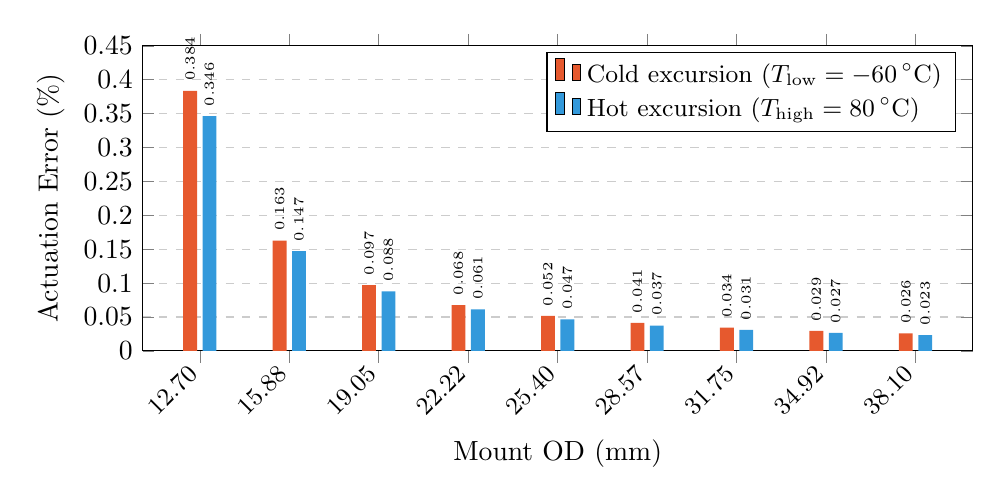
\begin{tikzpicture}
						\begin{axis}[
								ybar,
								bar width=5pt,
								width=\textwidth,
								height=0.45\textwidth,
								xlabel={Mount OD (mm)},
								ylabel={Actuation Error (\%)},
								xtick=data,
								xticklabels={12.70, 15.88, 19.05, 22.22, 25.40, 28.57, 31.75, 34.92, 38.10},
								x tick label style={rotate=45, anchor=east, font=\small},
								legend style={at={(0.98,0.98)}, anchor=north east, font=\small},
								legend cell align={left},
								ymajorgrids=true,
								grid style={dashed, gray!40},
								ymin=0,
								ymax=0.45,
								ytick={0, 0.05, 0.10, 0.15, 0.20, 0.25, 0.30, 0.35, 0.40, 0.45},
								yticklabel={\pgfmathprintnumber[fixed, precision=2]{\tick}},
								enlarge x limits=0.08,
								nodes near coords,
								nodes near coords style={font=\tiny, rotate=90, anchor=west},
								every node near coord/.append style={/pgf/number format/fixed, 
																										/pgf/number format/precision=3},
						]

						%% Hot excursion bars (Design 1) — plotted first
						\addplot[fill={rgb,255:red,230;green,89;blue,46}, draw=none] coordinates {
								(1, 0.3837)
								(2, 0.1628)
								(3, 0.0972)
								(4, 0.0677)
								(5, 0.0515)
								(6, 0.0413)
								(7, 0.0344)
								(8, 0.0294)
								(9, 0.0257)
						};

						%% Cold excursion bars (Design 1) — plotted second
						\addplot[fill={rgb,255:red,51;green,153;blue,219}, draw=none] coordinates {
								(1, 0.3464)
								(2, 0.1470)
								(3, 0.0877)
								(4, 0.0611)
								(5, 0.0465)
								(6, 0.0373)
								(7, 0.0310)
								(8, 0.0266)
								(9, 0.0232)
						};

						\legend{Cold excursion ($T_\text{low}=\SI{-60}{\degreeCelsius}$),
										Hot excursion ($T_\text{high}=\SI{80}{\degreeCelsius}$)}

						\end{axis}
					\end{tikzpicture}
					\caption{Actuator subsystem diameter optimization}
					\label{fig:mount_OD_opt}
				\end{figure}

				\begin{figure}[H]
					\centering
					\pgfplotstableread[col sep=comma]{csv/elastic_deformation.csv}\elasticdata
					\begin{tikzpicture}
						\begin{axis}[
								width=\textwidth,
								height=0.5\textwidth,
								xlabel={Wall thickness (mm)},
								ylabel={Total deflection ($\upmu$m)},
								xmin=0, xmax=12,
								ymin=0, ymax=1.0,
								ytick={0, 0.2, 0.4, 0.6, 0.8, 1.0},
								restrict y to domain=0:1.0,
								xtick={0,1,...,12},
								ymajorgrids=true,
								grid style={dashed, gray!40},
								legend style={
										at={(0.98,0.98)},
										anchor=north east,
										font=\small,
										cells={anchor=west}
								},
								clip=true,
						]

						%% ALLVAR tube (mount)
						\addplot[
								color={rgb,255:red,46;green,115;blue,178},
								mark=*,
								mark size=2.5pt,
								line width=1.5pt,
						] table[x=t_wall_mm, y=d_alv_max_um] {\elasticdata};
						\addlegendentry{ALLVAR tube (mount)}

						%% Al rod (actuator)
						\addplot[
								color={rgb,255:red,217;green,84;blue,26},
								mark=square*,
								mark size=2.5pt,
								line width=1.5pt,
						] table[x=t_wall_mm, y=d_al_max_um] {\elasticdata};
						\addlegendentry{Al rod (actuator)}

						%% Combined series
						\addplot[
								color={rgb,255:red,33;green,140;blue,33},
								mark=diamond*,
								mark size=3pt,
								line width=1.5pt,
						] table[x=t_wall_mm, y=d_ser_max_um] {\elasticdata};
						\addlegendentry{Combined series}

						%% Optimal wall thickness vertical line at 3.5 mm
						\draw[dashed, black, line width=1.2pt] (axis cs:3.5, 0) -- (axis cs:3.5, 1.0);

						%% Minimum point marker at (3.5, 0.1401)
						\addplot[
								only marks,
								mark=*,
								mark size=4pt,
								color=black,
						] coordinates {(3.5, 0.140052)};
						\addlegendentry{Series min @ $t_{\text{wall}} = \SI{3.5}{\milli\meter}$}

						\end{axis}
					\end{tikzpicture}
					\caption{Mount wall thickness optimization}
					\label{fig:mount_thick_opt}
				\end{figure}

			\subsubsection{Threaded Interface}
			\label{subsubsec:design:just:gen_dim:thread}

				As detailed by Sandia, gas will be supplied by a stainless steel pipe between \SI{1.524}{\milli\meter} and \SI{25.4}{\milli\meter} in diameter.
				This design features a \SI{19.05}{\milli\meter} (\nicefrac{3}{4}'') threaded interface, whose diameter can be adjusted in further design iterations as needed for particular experiments.

				The housing inlet and outlet provide \SI{15}{\milli\meter} and \SI{20}{\milli\meter} threaded length, respectively, for an airtight seal.
				Adding the space needed for the tapered drill-bit cut and the walls that support the valve orifice, the valve subsystem's longitudinal mechanical envelope totals \SI{72}{\milli\meter}, well within its design specification.

				\subsubsection{Assemblability Considerations}
			\label{subsubsec:design:just:gen_dim:assem}

				Manufacture and assembly of the \device\ motivated several features. The full assembly process is detailed in Appendix~\ref{app:mfg}.
				Every weld operation requires an orthogonal beam at all times.
				The housing center is broken into two pieces, allowing the bellows to be welded to the valve orifice and the housing centers separately with a full 360$^\circ$ line of sight.
				The subassembly can then be inserted into the housing inlet and welded in place from above, then fit to the housing outlet and welded from the outside.
				The actuator expansion rod is attached to the valve stem with a 360$^\circ$ weld.
				This is screwed to the mount, which is then welded to the housing.
				This modular approach allows for full line-of-sight welding and simple assembly and drove many of the structural features of the \device.

			\subsubsection{Valve Orifice Contact Friction}
			\label{subsubsec:design:just:gen_dim:friction}

			The interface between vertical faces of the valve orifice and the housing inlet are subject to frictional forces that could cause wear and galling (i.e. degradation of materials as their surfaces slide against one another), which could damage the system performance over time.
			To mitigate this, the contact surfaces are coated with a thin layer of Titanium Carbonitride (TiCN), a hard ceramic coating that provides excellent wear resistance and low friction properties.
			Compared to uncoated Invar, the TiCN coating provides a $5.6\!\times\!$ increase in hardness and a 63\% reduction in the wear rate under similar conditions\cite{ref_TiCN_Coating}.
			The coating is applied using Physical Vapor Deposition (PVD), a process that deposits a thin film $(\approx 2-4 \si{\micro\meter})$ of material onto the surface of the substrate.
			Figure~\ref{fig:coated_surfaces} depicts the coated surfaces.
			
			\begin{figure}[H]
				\centering
				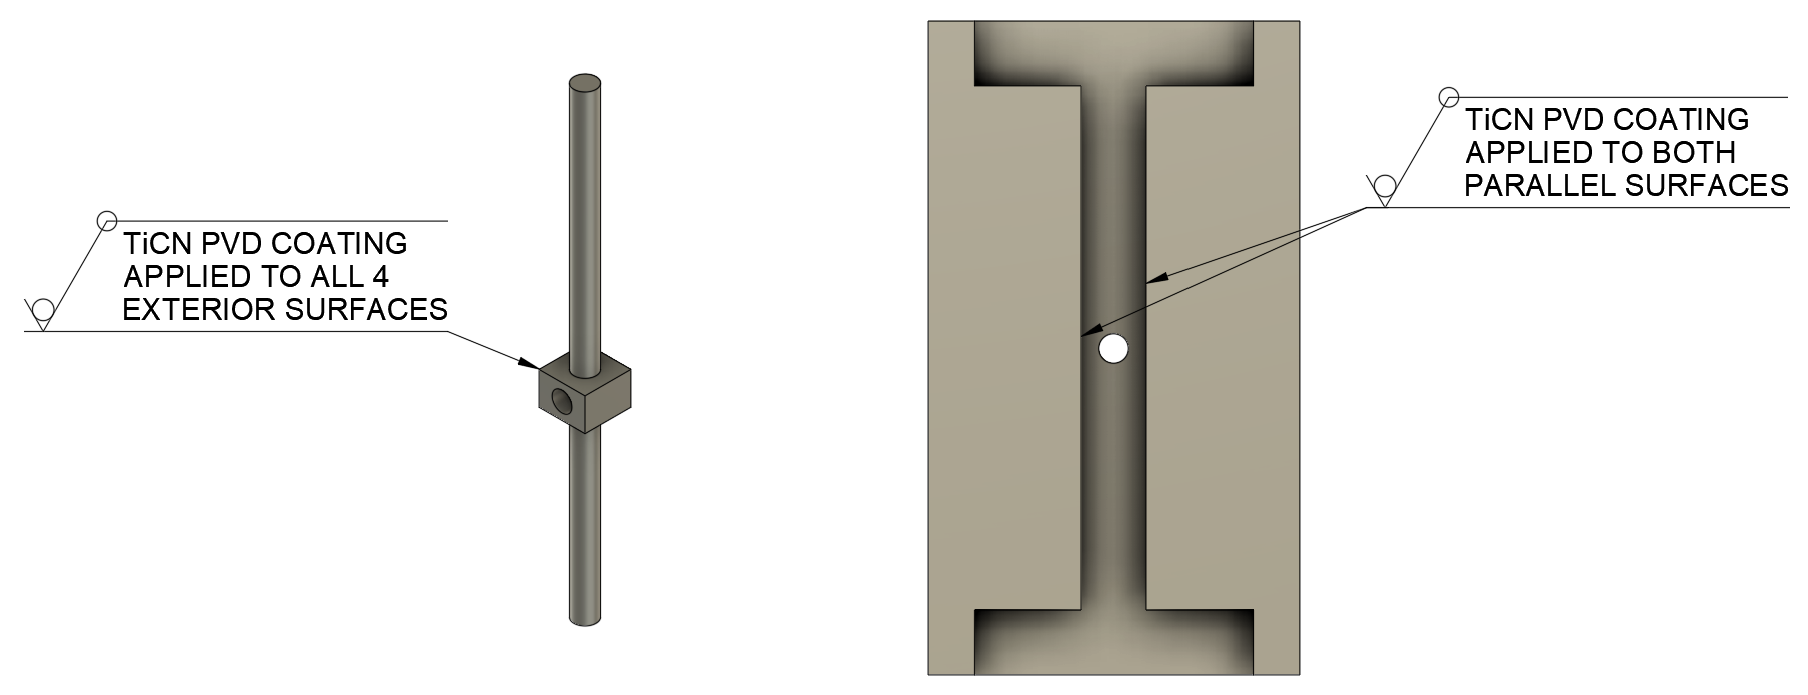
\includegraphics[width=.85\textwidth]{coated_surfaces.png}
				\caption{Target internal valve geometries selected for TiCN coating}
				\label{fig:coated_surfaces}
			\end{figure}

			\subsubsection{Mechanical Envelope Specifications}
			\label{subsubsec:design:just:gen_dim:ME}

				As stated in various sections above, each subsystem met its mechanical envelope specifications, with one exception: the valve subsystem violates its vertical mechanical envelope, pushing the total system height to $(\SI{45.55}{\milli\meter} + \SI{70.72}{\milli\meter}) = \SI{116.27}{\milli\meter}$, a 16\% violation of the required mechanical envelope.
				This was necessary to allow a direct interface between the actuator and valve subsystems, dramatically increasing the system precision compared to the complex mechanism required to make it more compact.
				As described in detail in Appendix~\ref{app:PM}, Sandia confirmed the precedence of the Required Relationship over the Mechanical Envelope,
				which is consistent with the system requirement obligation keywords emphasized in Section~\ref{sec:intro:req}.

				A few design changes, discussed in Section~\ref{chap:concl}, may allow the \device\ to fit within the Mechanical Envelope.
				These would slightly sacrifice precision. The impact of these changes could not be reliably evaluated during the initial design process,
				but the tools since developed and presented in Appendix~\ref{app:sat:TF} readily allow for a more informed trade-off analysis.

		\subsection{Calibration}
		\label{subsec:design:just:cal}

			Slight machining errors in every dimension will be present. Even those within their specified tolerance can endanger the system performance of the \device.
			Deviation from the intended thermal expansion rate cannot be adjusted post-manufacture, but any constant offset, such as from extra length in the valve stem, can be.
			The calibration stack, pictured in Figure~\ref{fig:cal}, allows the user to set the output of the device at a single temperature, shifting the whole system output closer to the center of its tolerance in satisfaction of Specification \specref{A.1.2}.
			The actuator subsystem is assembled and fastened using an M2 screw, which passes through the mount, supported by a flat washer, and threads into the central expansion rod.
			As the screw is tightened, a belleville washer between the two clamped faces maintains tension in the screw, letting the threads seat at any position within the belleville washer's range.
			See Appendix~\ref{app:calcs:cal:force} for further calculations and Appendix~\ref{app:mfg} for calibration instructions.
			Calibration ought to be performed at room temperature (approximately $T_{ref}$), where the required tolerance window is narrowest (cf. Appendix~\ref{app:calcs:orifice_geometry}).
			\vspace{1\baselineskip}
			\begin{figure}[H]
				\centering
				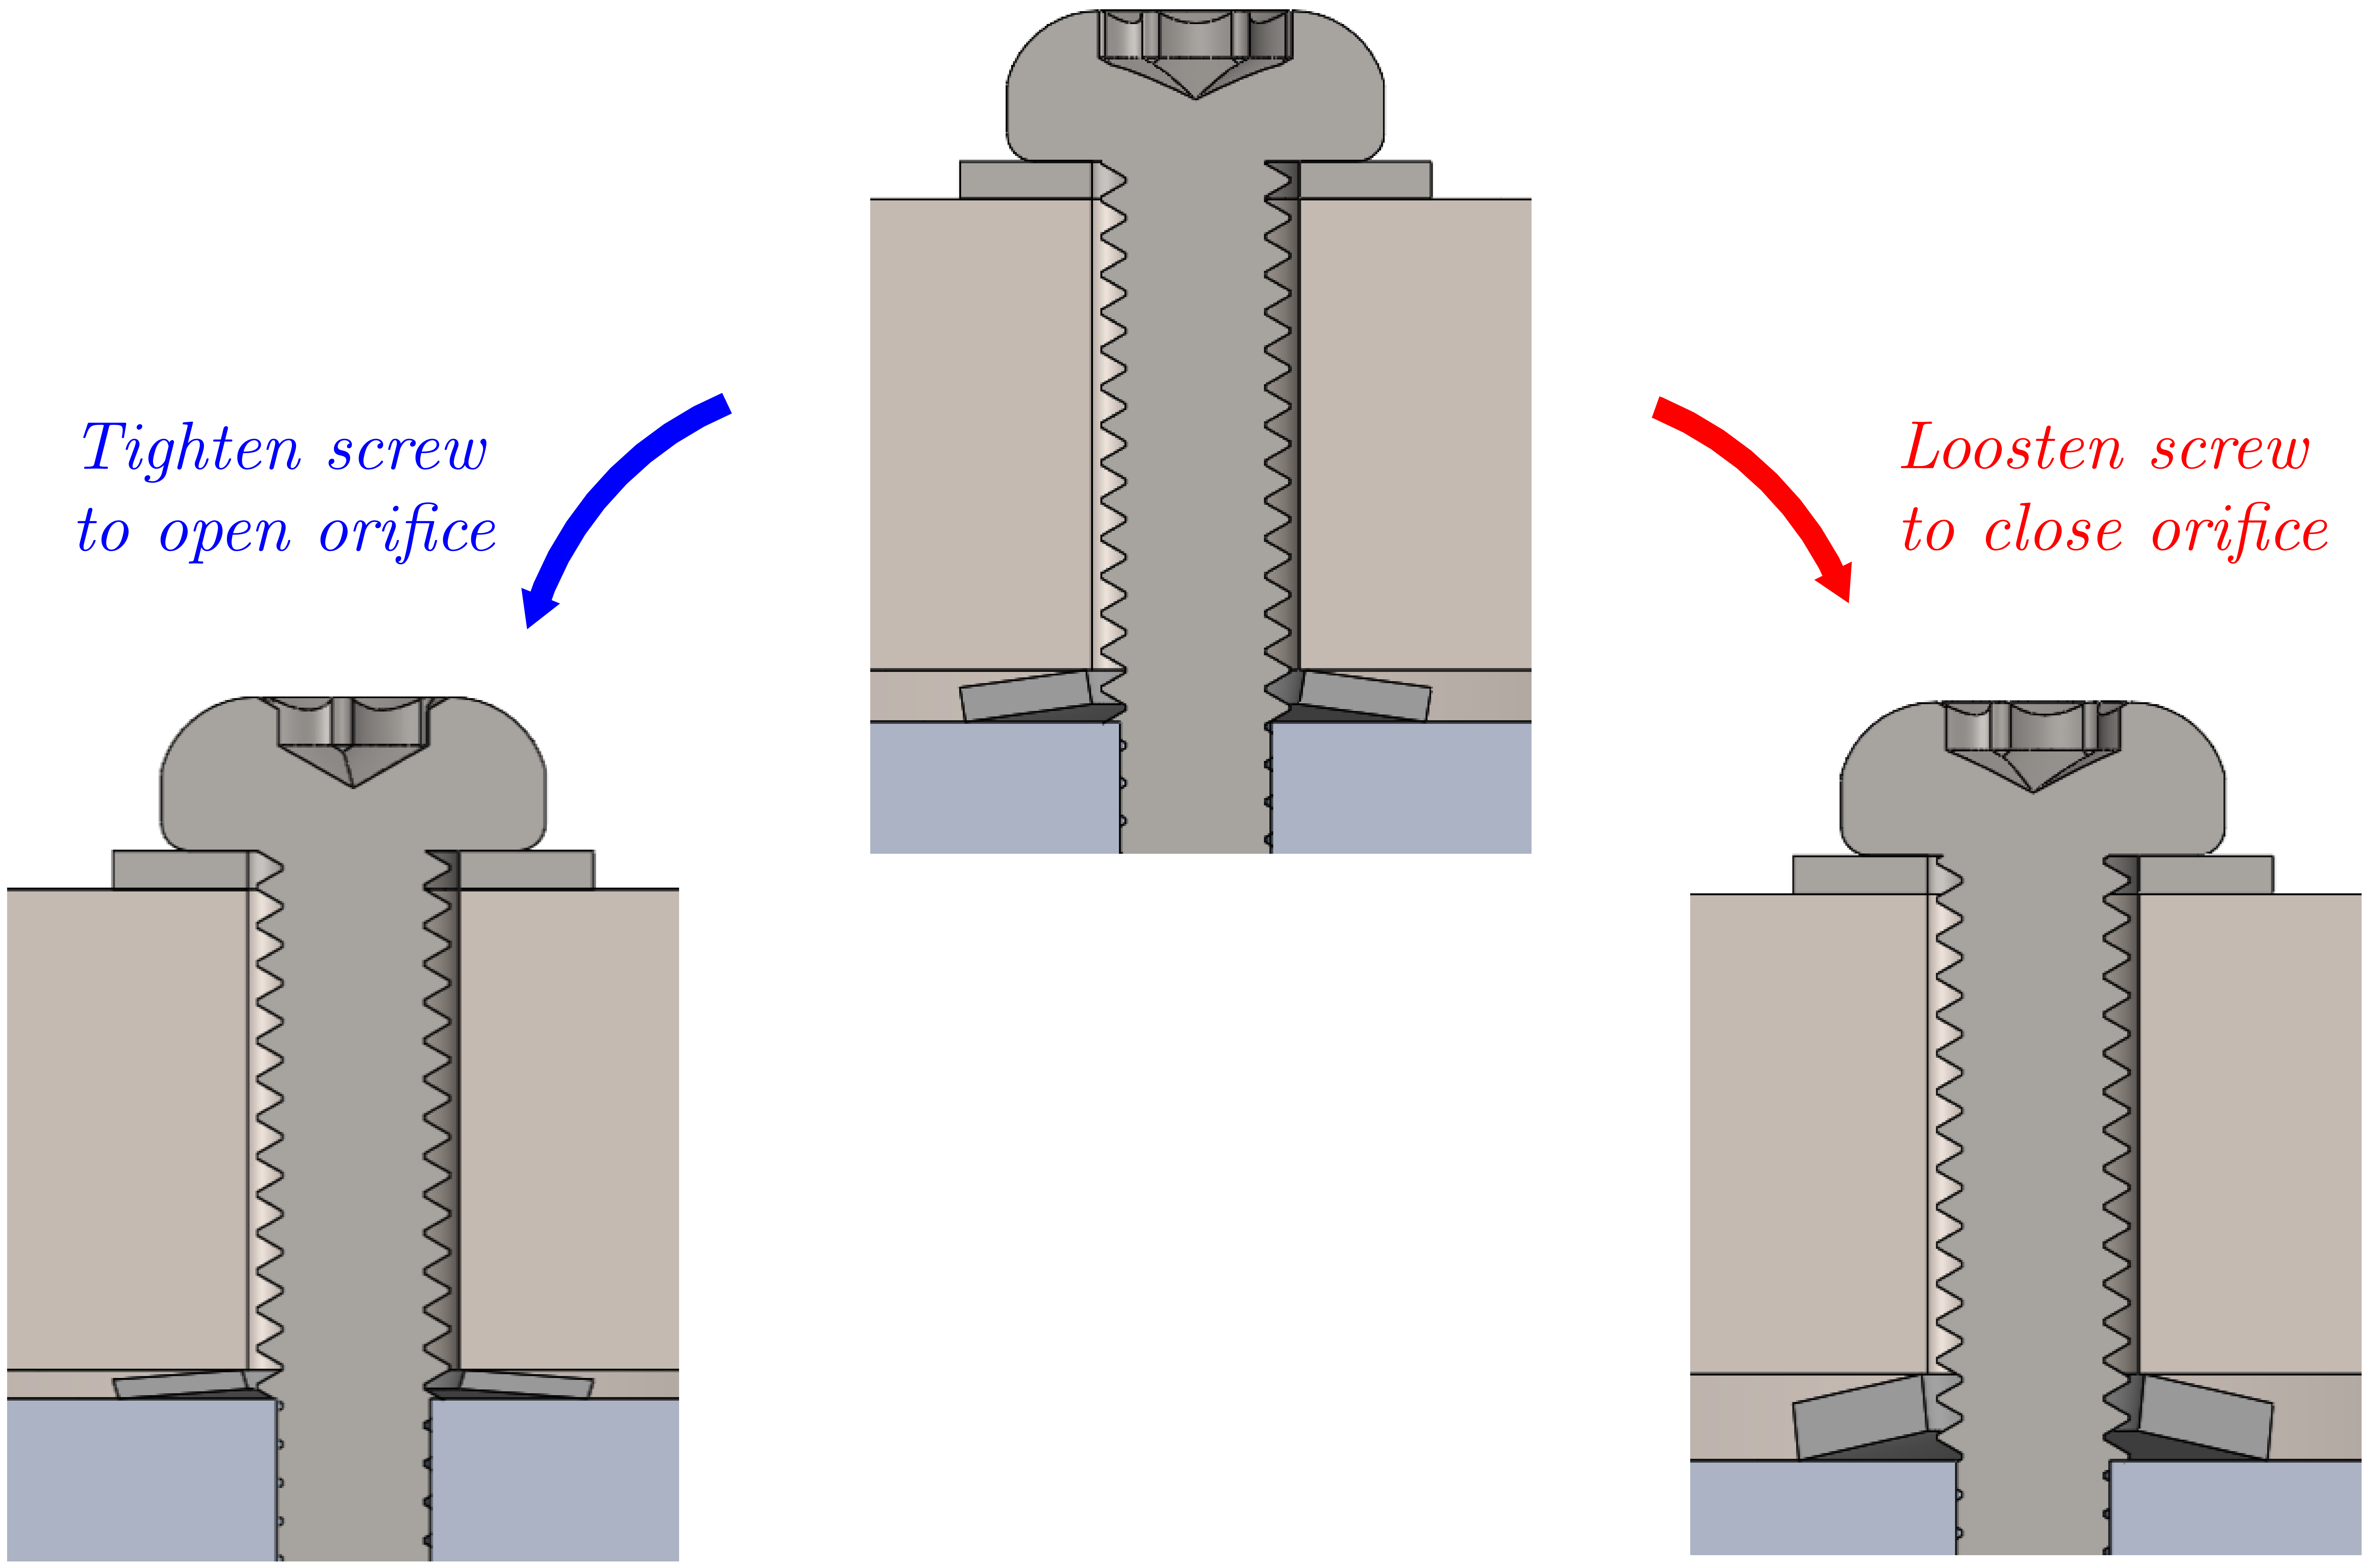
\includegraphics[width=.75\textwidth]{cal.png}
				\caption{System calibration with a belleville washer}
				\label{fig:cal}
			\end{figure}

		\subsection{Weld Joint Overview}
		\label{subsec:design:just:weld_overview}

		The \device\ is assembled using Electron Beam Welding (EBW), a high-precision welding 
		technique that uses a focused beam of electrons to join materials 
		together\cite{ref_steen2010laser}. EBW was selected for several reasons critical to 
		the \device's performance requirements. First, welding the entire assembly eliminates 
		mechanical fasteners and threaded interfaces, minimizing the degrees of freedom in the 
		final assembly and preventing the backlash and compliance introduced by alternative 
		joining methods. This directly improves system-level positioning precision, which is 
		essential given the tight tolerances required at the valve orifice. Second, EBW's high 
		power density enables complete fusion across the interface in a single pass, producing 
		full-penetration welds with a narrow heat-affected zone and minimal thermal distortion.
		This is critical for maintaining the dimensional tolerances of the precision fits 
		described in Section~\ref{subsec:design:just:fits}.

		The \device\ requires five different types of welds:

		\begin{itemize}
			\item Circumferential welds joining the bellows to the housing centers and the 
				valve orifice.
			\item Orthogonal welds joining the housing centers to the housing inlet.
			\item A circumferential weld joining the housing inlet and center pieces to the 
				housing outlet.
			\item A weld joining the actuator to the valve stem.
			\item A circumferential weld joining the mount to the housing.
		\end{itemize}

		Of these, the welds joining the housing inlet, outlet, and center pieces are the most 
		critical, as they form the pressure boundary of the valve and are subject to the highest 
		stresses. These joints use a square butt geometry, which is widely used in pressure 
		vessel construction and permits full penetration by EBW. Full penetration is considered 
		achieved when the weld fuses through the entire wall thickness $t$.

		Weld quality is verified using 100\% X-ray radiographic inspection per ASME 
		B31.3\cite[Table~302.3.4]{ref_asme_b313}. With all welds passing inspection 
		($E = 1.00$), no strength penalty relative to the base material is introduced, and the 
		joints are certified free of defects such as porosity, lack of fusion, and cracking, 
		all of which could significantly reduce joint strength\cite{ref_steen2010laser}. The 
		structural adequacy of the critical pressure-boundary welds is evaluated in 
		Section~\ref{sec:DFMEA:weld}.

		\subsection{Precision Fits}
		\label{subsec:design:just:fits}

			The \device\ features several components that will slide closely against one another, either once during assembly or repeatedly during operation.
			The tolerances of the inner and outer component, which are referred to as the ``shaft'' and ``hole'' (though not always circular), can be optimized according to the application's precision-friction trade-off. 
			Shigley's Mechanical Engineering Design\cite[Tables 7-9, A-11, A-12]{ref_shigley} establishes best practice for fit tolerances by fine-tuning the maximum and minimum tolerances of each hole and shaft dimension.
			For each of the following fits, the necessary balance between locational precision and frictionless movement yielded a particular fit type, which corresponds to a given code (e.g. H7/g6) for use in the engineering drawings.

			\begin{itemize}
				\item The actuator slides against the mount as it expands. To minimize deflection (see Section~\ref{subsubsec:design:just:gen_dim:act_diam}), the internal expansion rod should fully span the mount's bore diameter.
					However, sufficient clearance will ensure that their surfaces do not touch, especially as each expands laterally\footnote{ALLVAR is not isotropic. This means that although its vertical CTE is negative, its horizontal CTE values are positive like any ordinary metal. Thus, both components of the actuator will expand as they heat, building friction at their contact surfaces if not given sufficient clearance.}
					with temperature. A \textit{free running fit} (H9/d9) provides sufficient accuracy with enough clearance to avoid any friction.
				\item The valve stem must be machined to the bellows' exact convolution inner diameter to support it against pressure-driven squirm (see Section~\ref{subsec:design:just:bellows}), but like the actuator, contact should be avoided.
					Because Inconel and Invar expand far less than aluminum and ALLVAR, a closer fit can be afforded to prevent lateral movement.
					A \textit{sliding fit} (H7/g6) allows for low-friction movement at low speeds; it is the closest fit before contact occurs.
					While the bellows convolution inner diameter tolerance cannot be manipulated, a g6 tolerance on the valve stem will ensure minimal friction.
					Likewise, the hole in the housing center guides the valve stem's motion and requires the same tolerance (H7).
				\item The valve stem's lateral placement critically affects the orifice geometry; its fit must permit minimal side-to-side movement. However, as with the valve stem, a snug fit risks galling (see Section~\ref{subsubsec:design:just:gen_dim:friction}), which would allow for a buildup of static friction before movement occurs,
					so another \textit{sliding fit} (H7/g6) ensures free locational motion while maintaining light contact on all sides.
				\item The housing center should be snugly seated into the housing inlet upon assembly.
					After it is welded in place, friction will be irrelevant; thus, to locate the housing center's hole as precisely as necessary, a \textit{locational clearance fit} (H7/h6) will be applied.
			\end{itemize}

		\subsection{Material Selection}
		\label{subsec:design:just:mat}

		
			Each material selected for the \device\ enabled its exceptional performance despite impossible design circumstances.
			The Ashby Chart\cite{ref_ashby} (Figure~\ref{fig:ashby}), an engineering standard for thermal stress of materials, provides a fitting guide for the relative strength and thermal expansivity of various metals, polymers, and ceramics.
			Materials further up and to the right will possess greater driving authority when expanding, either by a higher CTE $\alpha$ or higher stiffness $E$.
			
			\begin{figure}[h]
				\centering
				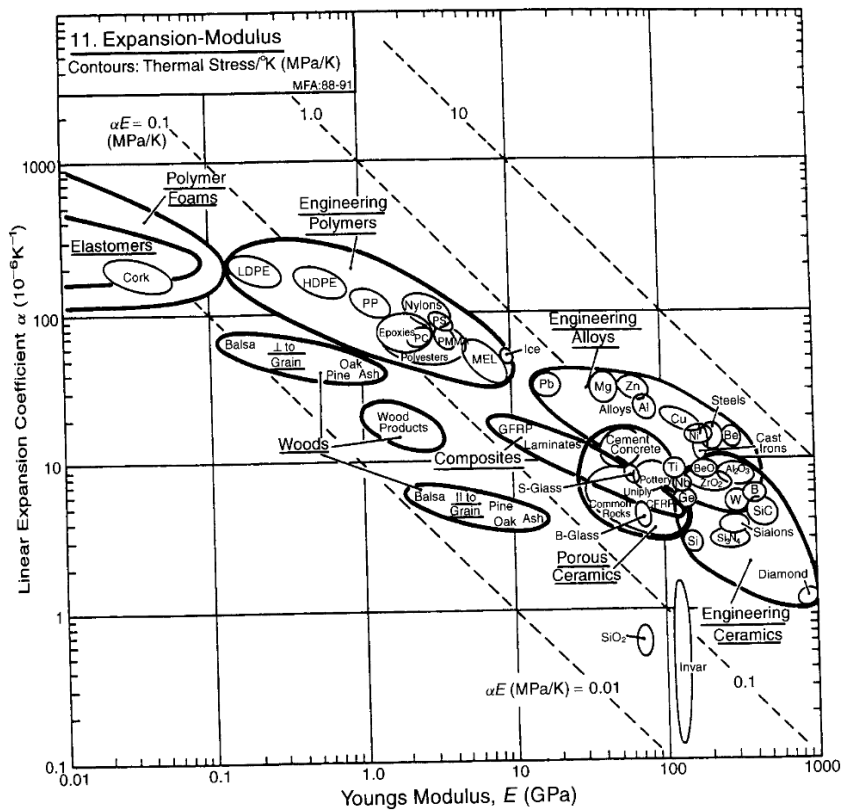
\includegraphics[width=.75\textwidth]{ashby.png}
				\caption{The Ashby Chart for metals, polymers, and ceramics}
				\label{fig:ashby}
			\end{figure}
			
			\subsubsection{Aluminum expansion rod}
			\label{subsubsec:design:just:mat:Al}

				The actuator expansion rod requires a high, stable thermal expansion rate to properly drive the valve stem.
				As reflected on the Ashby Chart, polymers possess the highest CTE, but they are soft (meaning they will readily deflect under reaction forces, such as from the bellows) and exhibit an inconsistent expansion rate across the full design temperature range.
				Ceramics, though they have a high thermal stiffness, will hardly expand due to their low CTE, and their high modulus of elasticity makes them nearly impossible to machine to the necessary tolerance.
				Some metals, such as certain Zinc and Magnesium alloys, have a CTE as high as \SI{30}{\micro\meter\per\meter\per\celsius}, but like the polymers, their expansion rates are too inconsistent for the precise output required by the \device.
				Aluminum\cite{ref_NASA_specs_Al} stands alone\footnote{
					This absolute must be taken with a grain of salt. While ALLVAR, Invar 36, and Inconel 718 show strong evidence that they are the best material choices for their respective applications, aluminum may be best replaced with a certain Zinc or Magnesium alloy.
					Its selection process was expedited due to time constraints. Further research may reveal an alloy with a consistent CTE higher than that of aluminum, allowing for a shorter bimetallic actuator.} 
				as a strong, expansive, consistent metal. It has a CTE of \specActuatorCTE\ at $T_{ref}$ that varies a maximum of \SI{1}{\micro\meter\per\meter\per\celsius} as $\SI{-60}{\celsius} \leq T_{amb} \leq \SI{80}{\celsius}$.

			\newpage
			\subsubsection{ALLVAR mount}
			\label{subsubsec:design:just:mat:ALLV}

				\begin{wrapfigure}{l}{.45\textwidth}
					\centering
					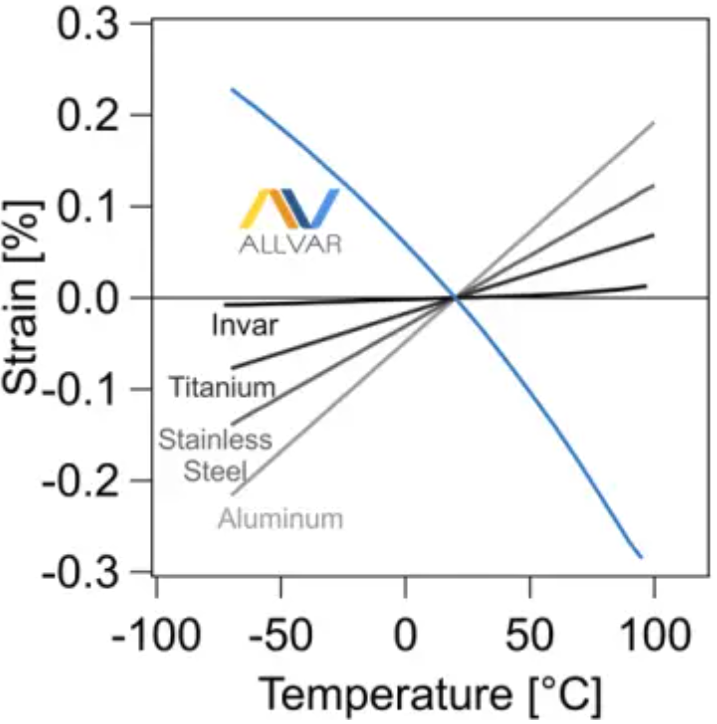
\includegraphics[width=.43\textwidth]{ALLVAR_CTE.png}
					\caption{CTE of ALLVAR against other metals}
					\label{fig:ALLVAR_CTE}
				\end{wrapfigure}

				ALLVAR Alloy 30\cite{ref_AllvarAlloys}, used for the mount as the second actuator metal, 
				is a proprietary, Titanium-based alloy patented by ALLVAR Alloys\cite{ref_AllvarAlloys_gen}.
				Unlike any other metal, it shrinks along one axis when heated, allowing for the compact bimetallic actuator design.
				Its CTE magnitude is even higher than that of aluminum and just as consistent\footnote{Although ALLVAR Alloys does not provide temperature-dependent thermal expansion data for their products, and although their thermal expansion data presented in Figure~\ref{fig:ALLVAR_CTE} is imprecise, they claim a mostly linear expansion rate across our whole design temperature range.}
				(Figure~\ref{fig:ALLVAR_CTE}\cite{ref_AllvarAlloys}).

				Several thermal switch designs\cite{ref_Bugby_2021, ref_Ralphs_2024, ref_Ralphs_2026}, which make use of a binary-output bimetallic actuator for aerospace heat-transfer applications, have used the ALLVAR-aluminum combination\footnote{The cited papers\cite{ref_Bugby_2021, ref_Ralphs_2024, ref_Ralphs_2026} were provided to our team directly by ALLVAR Alloys in support of their technology.},
				validating this combination.

				Furthermore, ALLVAR exhibits a low coefficient of thermal conductivity $(k = 8.88)$, providing thermal resistance to heat conducted through the valve housing.

			\subsubsection{Invar housing}
			\label{subsubsec:design:just:mat:Inv}

				Invar 36\textsuperscript{{\textregistered{}}}\cite{ref_Carpenter_Inv}, used for all machined parts in the valve subsystem, exhibits an exceptionally low coefficient of thermal expansion.
				Swiss physicist and metrologist Charles \'{E}douard Guillaume unexpectedly discovered the exotic metal Invar, short for ``\textit{invariable}'', in 1897\cite{ref_Invar_1897}.
				He won a Nobel Prize for this discovery in 1920\footnote{
					The curious individual may find Guillaume's 1920 Nobel Prize lecture\cite{ref_Invar_1920} particularly fascinating.
				}\cite{ref_Invar_1920}.
				Carpenter Technology\cite{ref_Carpenter_gen}, a manufacturer of the alloy, now holds the registered trademark to the name Invar 36 and confirms that its CTE reaches no more than \specInvarCTE\ within the design temperature range\cite{ref_Carpenter_Inv},
				ten times less than that of steel\cite{ref_ASM_Steel} and 20 times less than aluminum\cite{ref_NASA_specs_Al}.
				This special property allows exceptional thermal stability in the parts not designed to expand, allowing for precise thermomechanical performance.
				The Ashby Chart (Figure~\ref{fig:ashby}) makes apparent that Invar stands alone as a low-expansion metal. Only ceramics, which are too hard to machine, approach its expansion rate.
				Invar is plotted with such an eccentric ellipse, not because its CTE is inconsistent across temperature, but because myriad heat-treatment and work-hardening processes can bring its CTE as low as \SI{0.15}{\micro\meter\per\meter\per\celsius}.
				Guillaume claimed to have brought one sample of Invar wire several kilometers long to a negative CTE, annealed it back to near-zero, and found its expansion rate imperceptible even at that length\cite[p.~452]{ref_Invar_1920}.

				Invar, like ALLVAR, resists thermal conduction $(k = 10.5)$. Heat transfer between the heated gas and the actuator subsystem is better inhibited than it would be by other metals.

			\subsubsection{Inconel bellows}
			\label{subsubsec:design:just:mat:Inc}

				INCONEL\textsuperscript{{\textregistered{}}}\cite{ref_SpecialMetals_Inc} Alloy 718, a Nickel superalloy used by Mini-Flex for their high-pressure bellows, outperforms any other metal on several key metrics as a hermetic seal and is ubiquitous in the aerospace industry\cite[p.~1]{ref_SpecialMetals_Inc}.
				Special Metals Corporation\cite{ref_SpecialMetals_gen} now holds the registered trademark\footnote{
					Inconel, like Invar, was discovered by mistake, this time by American metallurgist Herbert Louis Eiselstein for INCO in 1965\cite{ref_Inconel_1965}.
					Curious readers will find his account of the discovery (given at a metallurgy conference in 1991) compelling\cite{ref_Inconel_1991}.}.
				Its CTE and Elastic Modulus are unspectacular and near that of steel.
				Nevertheless, such conventional metals fail several criteria required to meet and maintain Specifications \specref{V.3.2} and \specref{V.3.3}:

				\begin{itemize}
					\item \textbf{Strength at temperature.} All metals soften when heated and embrittle when chilled. Inconel, according to its developer, is ``suitable for temperatures from [\SI{-250}{\celsius}] up to [\SI{700}{\celsius}]''%
						\footnote{Converted from \textdegree F}\cite[p.~62, 74--76]{ref_Inconel_1965}.
					\item \textbf{Fatigue resistance.} Metals wear under repeated cyclic loads typical of a bellows. Inconel outlasts most metals under such conditions, reported to have ``Good tensile, fatigue, creep, and rupture strength'' by its manufacturer\cite[p.~1]{ref_SpecialMetals_Inc}.
					\item \textbf{Hydrogen compatibility.} All gases diffuse (penetrate) through all metals imperceptibly. Hydrogen does this particularly aggressively, leading to embrittlement, the loss of a metal's ductility as its material reacts with the seeping gas.
						Inconel, though an imperfect barrier, is especially immune to this phenomenon. Jonathan Lee, writing for NASA in 2016\cite[Table~4]{ref_NASA_Inc}, rated Inconel 718 as ``Extreme'' on the Hydrogen Environmental Embrittlement (HEE) scale at conditions up to \SI{68.9}{\mega\pascal}.
					\item \textbf{Weldability.} Prior to the development of Inconel 718, the leading precipitation-hardened Nickel superalloys used in the industry all suffered from heat embrittlement, causing them to crack. Inconel, found to be particularly suitable for Electron Beam welds, drove the alloy's industry dominance.
				\end{itemize}

				See Appendix~\ref{app:datasheets:mat} for relevant material data used throughout this report.

\chapter{Mission: Accomplished}
\label{chap:concl}

	The Passive Temperature Compensation Device presented in this design report combines proven, robust technology with a novel valve-orifice architecture
	to accomplish thermomechanical flow control with greater precision than has been achieved before.
	By only allowing flow through the overlap between two diamond holes pressed flush against one another, one mobile and one fixed,
	the \device\ can produce first-order variations in its effective orifice diameter with a single moving part.
	These square holes can be manufactured with very sharp corners using Wire Electrical Discharge Machining.
	An external bimetallic thermal actuator drives these changes with compound mechanical displacement.
	Its interface is hermetically sealed with minimal mechanical or fluid resistance using two flexible metal bellows.
	Specialized materials and precise Electron Beam Welding maximize thermal stability, strength, and compactness.
	This proof-of-concept model provides Sandia National Laboratories with the necessary design foundation for development of a working physical prototype
	and customization of the design for specific experiments.

	The design process is unfinished. As intended, only the first iteration was fully developed.
	The computational prototype presented in this report demonstrates the feasibility of the \device\ and provides convenient tools for further iteration.
	Appendix~\ref{app:iter:weak} provides an exhaustive list of identified weaknesses, unaddressed assumptions, and revisions the authors would implement in the second design iteration.
	In summary, not all error modes could be accounted for in Chapter~\ref{chap:DFMEA},
	leading to an optimistic estimation of the device's performance. Full verification will not be complete until Sandia revises this design, builds a physical prototype, and tests it.
	Appendix~\ref{app:iter:customize} provides them with guidance on how to use the computational tools presented in Chapters~\ref{chap:DFMEA} and \ref{chap:test} for the revision before a physical prototype is built,
	affording a more informed trade-off analysis between satisfaction of the Required Relationship and smaller priorities such as size, cost, and longevity.

	This first-iteration design of the \device\ demonstrates feasibility as a high-precision thermomechanical valve. Once revised, prototyped, and tested by Sandia, it can provide reliable, passive experimental flow regulation without depending on external power or computation,
	streamlining experimental control and improving the accuracy and repeatability of their research.


% \chapter*{} % Bibliography without extra header
\addcontentsline{toc}{chapter}{Bibliography}

\begin{thebibliography}{99}

	\bibitem{ref_finalDesignReport} % Report 3
	S.\ van der Veen, M.\ Cuaycong, N.\ Metta, J.\ Pizarro, I.\ Mathew, and J.\ Bodine,
	``Passive Temperature Compensation Device --- Final Design Report,''
	Noble Aggie Labs, University of California, Davis, CA, Jun.\ 5, 2026. [Unpublished].

	\bibitem{ref_ASHRAE_thermostatic}
	R.\ McDowall, \textit{Fundamentals of HVAC Control Systems}, I-P ed.,
	American Society of Heating, Refrigerating and Air-Conditioning Engineers,
	Atlanta, GA, 2009, Sec.~1.2.

	\bibitem{ref_Vernet_1938}
	S.\ Vernet, ``Thermostat,'' U.S. Patent 2\,115\,501, Apr.\ 26, 1938.
	Available: \url{https://patents.google.com/patent/US2115501}
	[Accessed: May 11, 2026].

	\bibitem{ref_Bugby_2021}
	D.\ C.\ Bugby, J.\ G.\ Rivera, S.\ L.\ Mauro, and J.\ T.\ Farmer,
	``Extended Stroke and Miniaturized Reverse-Operation DTE Thermal Switches,''
	\textit{50th Int.\ Conf.\ on Environmental Systems}, ICES-2021-412, Jul.\ 2021.

	\bibitem{ref_Ralphs_2024}
	M.\ Ralphs, M.\ Sinfield, M.\ Jensen, and M.\ Felt,
	``Passive Cryogenic Thermal Switch with Tunable Close Temperature for
	Redundant Cryocooler Systems,''
	\textit{Cryocoolers 23}, R.\ G.\ Ross, Jr. and J.\ R.\ Raab, Eds.,
	International Cryocooler Conference, Inc., Boulder, CO, 2024, pp.~389--394.

	\bibitem{ref_Ralphs_2026}
	M.\ I.\ Ralphs, M.\ Jensen, A.\ Eames, and M.\ Sinfield,
	``A Suite of Thermal Switches for Surviving Extreme Thermal Environments in Space,''
	\textit{AIAA SciTech 2026 Forum}, Orlando, FL, Jan.\ 2026,
	doi: 10.2514/6.2026-1086.

	\bibitem{ref_NIH}
	F.-C.\ Yang, Y.\ Zhang, and M.\ C.\ Rheinstädter,
	``The Structure of People's Hair,''
	\textit{PeerJ}, vol.~2, p.~e619, Oct.\ 2014. doi: 10.7717/peerj.619.

	\bibitem{ref_sandiaprompt}
	B.\ Bon,
	``Passive Temperature Compensation Device --- Project Prompt,''
	Sandia National Laboratories, SAND2025-15446O, 2025. [Unpublished].

	\bibitem{ref_NASA_specs_guide}
	National Aeronautics and Space Administration,
	\textit{NASA Systems Engineering Handbook}, NASA/SP-2016-6105 Rev2,
	Washington, DC: NASA, 2016, Sec.~4.2.

	\bibitem{ref_Nise}
	N.\ S.\ Nise, \textit{Control Systems Engineering},
	8th~ed., Hoboken, NJ: Wiley, 2019.

	\bibitem{ref_Invar_1897}
	C.-\'{E}.\ Guillaume,
	``Recherches sur les aciers au nickel. Dilatations aux temp\'{e}ratures
	\'{e}lev\'{e}es; r\'{e}sistance \'{e}lectrique,''
	\textit{Comptes Rendus de l'Acad\'{e}mie des Sciences},
	vol.~125, pp.~235--238, 1897.

	\bibitem{ref_Invar_1920}
	C.-\'{E}.\ Guillaume, ``Invar and Elinvar,'' Nobel Lecture,
	Nobel Prize in Physics, Stockholm, Sweden, Dec.\ 11, 1920.
	Available: \url{https://www.nobelprize.org/prizes/physics/1920/guillaume/lecture/}
	[Accessed: May 8, 2026].

	\bibitem{ref_shigley}
	J.\ E.\ Shigley, C.\ R.\ Mischke, and R.\ G.\ Budynas,
	\textit{Mechanical Engineering Design},
	8th~ed., New York, NY: McGraw-Hill, 2006.

	\bibitem{ref_wilton_hermetic}
	D.\ Wilton, ``Hermetic seal,'' \textit{Wordorigins.org}, Dec.\ 29, 2020.
	[Online]. Available: \url{https://www.wordorigins.org/big-list-entries/hermetic-seal}
	[Accessed: Jun.\ 2, 2026].

	\bibitem{ref_gesner_1559}
	K.\ Gesner, \textit{The Treasure of Euonymus Conteyninge the Wonderfull Hid
	Secretes of Nature}, P.\ Morwyng, trans., London: John Daie, 1559, p.~66.

	\bibitem{ref_Young_Freedman}
	H.\ D.\ Young and R.\ A.\ Freedman,
	\textit{University Physics with Modern Physics},
	15th~ed., Hoboken, NJ: Pearson, 2019, Eq.~6-8.

	\bibitem{ref_miniflex_catalog}
	Mini-Flex Corporation, \textit{2026 Metal Bellows Catalog},
	Mini-Flex Corporation, Watervliet, NY. [Online].
	Available: \url{https://mini-flex.com/metal-bellows-catalog/}
	[Accessed: Feb.\ 23, 2026].

	\bibitem{ref_miniflex_design}
	Mini-Flex Corporation, \textit{Metal Bellows Design Guide},
	Mini-Flex Corporation, Watervliet, NY. [Online].
	Available: \url{https://mini-flex.com/metal-bellows-design-guide/}
	[Accessed: Feb.\ 23, 2026].

	\bibitem{ref_TiCN_Coating}
	T.\ Lv, T.\ Luo, T.\ Cheng, X.\ Hu, Z.\ Zhang, Z.\ Tang, B.\ Lin, and H.\ Xiao,
	``Microstructure and wear behavior of Invar alloy surface strengthened by
	{TiAl} laser alloying and {TiCN} ceramics,''
	\textit{Surface and Coatings Technology}, vol.~520, p.~132977, 2026.
	doi: 10.1016/j.surfcoat.2025.132977.

	\bibitem{ref_steen2010laser}
	W.\ M.\ Steen and J.\ Mazumder, \textit{Laser Material Processing},
	4th~ed., London, UK: Springer, 2010.

	\bibitem{ref_asme_b313}
	American Society of Mechanical Engineers,
	\textit{ASME B31.3: Process Piping},
	ASME, New York, NY, 2022.

	\bibitem{ref_ashby}
	M.\ F.\ Ashby, \textit{Materials Selection in Mechanical Design},
	5th~ed., Oxford, UK: Pergamon Press, 1992, Fig.~3.13.

	\bibitem{ref_NASA_specs_Al}
	R.\ F.\ Muraca and J.\ S.\ Whittick,
	\textit{Materials Data Handbook: Aluminum Alloy 6061}, 2nd~ed.,
	Western Applied Research \& Development, Inc., NASA CR-123772, May 1972.

	\bibitem{ref_AllvarAlloys}
	ALLVAR Alloys, \textit{What is Negative Thermal Expansion?},
	ALLVAR Alloys, 2026. [Online].
	Available: \url{https://allvaralloys.com/negative-coefficient-of-thermal-expansion-products-applications/round-bar-and-tube/}
	[Accessed: May 8, 2026].

	\bibitem{ref_AllvarAlloys_gen}
	ALLVAR Alloys, \textit{Negative Thermal Expansion. Positive Results.}\
	ALLVAR Alloys, 2026. [Online].
	Available: \url{https://www.allvaralloys.com/}
	[Accessed: May 9, 2026].

	\bibitem{ref_Carpenter_Inv}
	Carpenter Technology Corporation, \textit{Invar 36 Datasheet},
	Carpenter Technology Corporation, 2025. [Online].
	Available: \url{https://www.carpentertechnology.com/hubfs/7407324/Material%20Saftey%20Data%20Sheets/Invar%2036.pdf}
	[Accessed: May 8, 2026].

	\bibitem{ref_Carpenter_gen}
	Carpenter Technology Corporation, \textit{Global Leader in Specialty Alloys},
	Carpenter Technology Corporation, 2026. [Online].
	Available: \url{https://www.carpentertechnology.com/}
	[Accessed: May 8, 2026].

	\bibitem{ref_ASM_Steel}
	F.\ Cverna, Ed., \textit{ASM Ready Reference: Thermal Properties of Metals},
	ASM International, Materials Park, OH, 2002, Table~2.2.

	\bibitem{ref_SpecialMetals_Inc}
	Special Metals Corporation, \textit{INCONEL\textregistered{} Alloy 718},
	Publication No.\ SMC-045, Special Metals Corporation, 2007. [Online].
	Available: \url{https://www.specialmetals.com/documents/technical-bulletins/inconel/inconel-alloy-718.pdf}
	[Accessed: Apr.\ 17, 2026].

	\bibitem{ref_SpecialMetals_gen}
	Special Metals Corporation, \textit{High-Performance Alloy Products},
	Special Metals Corporation, 2026. [Online].
	Available: \url{https://www.specialmetals.com/}
	[Accessed: May 8, 2026].

	\bibitem{ref_Inconel_1965}
	H.\ L.\ Eiselstein,
	``Metallurgy of a Columbium-Hardened Nickel-Chromium-Iron Alloy,''
	in \textit{Advances in the Technology of Stainless Steel and Related Alloys},
	ASTM Special Technical Publication 369,
	American Society for Testing and Materials, Philadelphia, 1965, pp.~62--79.

	\bibitem{ref_Inconel_1991}
	H.\ L.\ Eiselstein and D.\ J.\ Tillack,
	``The Invention and Definition of Alloy 625,''
	in \textit{Superalloys 718, 625 and Various Derivatives},
	E.\ A.\ Loria, Ed., The Minerals, Metals \& Materials Society,
	Warrendale, PA, 1991, pp.~1--14.

	\bibitem{ref_NASA_Inc}
	J.\ A.\ Lee, \textit{Hydrogen Embrittlement},
	NASA Technical Memorandum NASA/TM-2016-218602,
	NASA Marshall Space Flight Center, Huntsville, AL, 2016.

	\bibitem{ref_Hibbeler}
	R.\ C.\ Hibbeler, \textit{Mechanics of Materials},
	9th~ed., Saddle River, NJ: Pearson, 2014.

	\bibitem{ref_beam}
	A.\ Grishin, ``Thin-Wall Rectangular Pressure Vessels Simulation,''
	Phoenix Analysis \& Design Technologies (PADT), Inc.,
	Tempe, AZ, USA, White Paper, Jun.\ 30, 2024. [Online].
	Available: \url{https://www.padtinc.com/wp-content/uploads/2024/06/thinwall_rectangular_pressure_vessels.pdf}
	[Accessed: May 29, 2026].

	\bibitem{ref_COMSOL}
	COMSOL~AB, \textit{COMSOL Multiphysics\textregistered{} Reference Manual},
	v.~5.3a, COMSOL~AB, Stockholm, Sweden, 2017.

	\bibitem{ref_sf}
	U.S.\ Department of Defense,
	\textit{MIL-STD-1522A: Standard General Requirements for Safe Design and
	Operation of Pressurized Missile and Space Systems},
	Department of Defense, Washington, DC, 1984, Table~III.

	\bibitem{ref_McMaster_belle}
	McMaster-Carr, \textit{316 Stainless Steel Spring Lock Washer,
	Part No.\ 93237A101}, McMaster-Carr Supply Company, 2026. [Online].
	Available: \url{https://www.mcmaster.com/93237A101/}
	[Accessed: May 8, 2026].

	\bibitem{ref_din6796}
	Deutsches Institut f\"{u}r Normung,
	\textit{DIN 6796: Conical Spring Washers for Bolted Connections},
	DIN, Berlin, 2009.

	\bibitem{ref_dinen16983}
	Deutsches Institut f\"{u}r Normung,
	\textit{DIN EN 16983: Disc Springs---Calculation}, DIN, Berlin, 2017.

	\bibitem{ref_dinen16984}
	Deutsches Institut f\"{u}r Normung,
	\textit{DIN EN 16984: Disc Springs---Quality Specifications---Dimensions},
	DIN, Berlin, 2017.

	\bibitem{ref_almen1936}
	J.\ O.\ Almen and A.\ Laszlo,
	``The Uniform-Section Disk Spring,''
	\textit{Transactions of the American Society of Mechanical Engineers},
	vol.~58, no.~4, pp.~305--314, 1936.

	\bibitem{ref_Ledbetter_Stainless}
	H.\ M.\ Ledbetter,
	``Stainless-Steel Elastic Constants at Low Temperatures,''
	\textit{Journal of Applied Physics}, vol.~52, no.~3, pp.~1587--1589, 1981.

	\bibitem{ref_jones1992}
	L.\ A.\ Jones, I.\ W.\ Hunter, and R.\ J.\ Irwin,
	``Differential thresholds for limb movement measured using adaptive techniques,''
	\textit{Perception \& Psychophysics}, vol.~52, no.~5, pp.~529--535, 1992.

	\bibitem{ref_Cappello2015}
	L.\ Cappello, N.\ Elangovan, S.\ Contu, S.\ Khosravani, J.\ Konczak,
	and L.\ Masia,
	``Robot-aided assessment of wrist proprioception,''
	\textit{Frontiers in Human Neuroscience}, vol.~9, article~198, Apr.\ 2015.
	doi: 10.3389/fnhum.2015.00198.

	\bibitem{ref_SNL}
	Sandia National Laboratories, \textit{About Sandia},
	Sandia National Laboratories, 2026. [Online].
	Available: \url{https://www.sandia.gov/about/}
	[Accessed: May 30, 2026].

	\bibitem{ref_haas}
	Haas Automation, Inc.,
	``VF-2: 40-Taper Standard Vertical Mill Specifications,''
	\textit{Haas Automation}. [Online].
	Available: \url{https://www.haascnc.com/machines/vertical-mills/vf-series/models/small/vf-2.html}
	[Accessed: May 16, 2026].

	\bibitem{ref_Jensen}
	N.\ Grønbech-Jensen,
	\textit{Introduction to Numerical Methods and Analysis}.
	[Unpublished].

	\bibitem{ref_Stewart}
	J.\ Stewart, \textit{Single Variable Calculus: Early Transcendentals},
	6th~ed., Belmont, CA: Thomson Brooks/Cole, 2008, p.~736; see also p.~674.

	\bibitem{ref_Anton}
	H.\ Anton and A.\ Kaul, \textit{Elementary Linear Algebra},
	12th~ed., Hoboken, NJ: Wiley, 2019, p.~228.

	\bibitem{ref_AIAG2005}
	Automotive Industry Action Group (AIAG),
	\textit{Statistical Process Control (SPC) Reference Manual},
	2nd~ed., AIAG, Southfield, MI, 2005, pp.~104, 132.

	\bibitem{ref_figliola}
	R.\ S.\ Figliola and D.\ E.\ Beasley,
	\textit{Theory and Design for Mechanical Measurements},
	5th~ed., Hoboken, NJ: Wiley, 2011, Sec.~4.9.

	\bibitem{ref_white}
	F.\ M.\ White and H.\ Xue,
	\textit{Fluid Mechanics}, 9th~ed.,
	New York, NY: McGraw-Hill Education, 2021.

	\bibitem{ref_McMaster_screw}
	McMaster-Carr, \textit{18-8 Stainless Steel Pan Head Torx Screws,
	Part No.\ 90362A141}, McMaster-Carr Supply Company, 2026. [Online].
	Available: \url{https://www.mcmaster.com/90362A141/}
	[Accessed: May 8, 2026].

	\bibitem{ref_McMaster_std}
	McMaster-Carr, \textit{18-8 Stainless Steel General Purpose Washer,
	Part No.\ 93475A195}, McMaster-Carr Supply Company, 2026. [Online].
	Available: \url{https://www.mcmaster.com/93475A195/}
	[Accessed: May 8, 2026].

\end{thebibliography}


\newpage
\begin{appendices}
\appendix

\chapter{Calculations and Supplemental Information}
\label{app:calcs}

	\section{Required Relationship: Tolerable Error}
	\label{app:calcs:errorProp}

		As detailed in Section~\ref{sec:intro:req}, the Required Relationship

			$$ \requiredRelationship $$

		depends on the following independent variables, each with their own tolerance values:

			\begin{align*}
				&A_1 = \Aone
				\\
				&A_0 = \Azero
			\end{align*}

		The tolerance of $D_{\text{effective}}$ as a function of temperature can be found using the following formula:

			\begin{equation}
				D_{\text{eff}} = \overline{D_{\text{eff}}}(T) \pm u_D(T)
				\label{eq:error_gen}
			\end{equation}

		where

			\begin{equation}
				u_D(T) =
				\begin{cases}
					- (5 \%) A_1 (T - T_{ref}) + (5 \%) A_0 & T \geq T_{ref} \\
					 (5 \%) A_1 (T - T_{ref}) + (5 \%) A_0 & T < T_{ref}
				\end{cases}
				\label{eq:error_particular}
			\end{equation}

		Because $A_1 < 0$ and the sign of $T - T_{ref}$ changes at $T = T_{ref}$, the $A_1$ error term must be reversed for higher temperatures.
		Combining Equations \eqref{eq:error_gen} and \eqref{eq:error_particular}, we find the range allowed by the Required Relationship across the whole temperature spectrum, represented in Table~\ref{tab:RR} and Figure~\ref{fig:RR}.

		\begin{table}[H]
			\centering
			\caption{Required Relationship nominal and tolerance values across the design space}
			\label{tab:RR}
			\begin{tabular}{ccc}
				\toprule
				$T$ (\textdegree C) & $D$ (\si{\micro\meter}) & $u_D$ (\si{\micro\meter}) \\
				\midrule
				$-60$ & 383.5 & 19.18 \\
				$-50$ & 368.3 & 18.42 \\
				$-40$ & 353.1 & 17.65 \\
				$-30$ & 337.8 & 16.89 \\
				$-20$ & 322.6 & 16.13 \\
				$-10$ & 307.3 & 15.37 \\
				$0$   & 292.1 & 14.61 \\
				$10$  & 276.9 & 13.84 \\
				$20$  & 261.6 & 13.08 \\
				$25$  & 254.0 & 12.70 \\
				$30$  & 246.4 & 13.08 \\
				$40$  & 231.1 & 13.84 \\
				$50$  & 215.9 & 14.61 \\
				$60$  & 200.7 & 15.37 \\
				$70$  & 185.4 & 16.13 \\
				$80$  & 170.2 & 16.89 \\
				\bottomrule
			\end{tabular}
		\end{table}

		\vspace{1em}

		Observe that the error boundary is thinnest about $T_{ref}$; thus, performance is best served if the \device\ is manufactured, assembled, and calibrated near this temperature.
		See Appendix~\ref{app:mfg} for more details.

	\section{Orifice Geometry}
	\label{app:calcs:orifice_geometry}

		The orifice, as defined in Section~\ref{sec:design:overview} and depicted in Figure~\ref{fig:orifice} (shown again in Figure~\ref{fig:orifice_rep}), is the ``Venn''-style overlap between two angled squares.

		\begin{figure}[H]
			\centering
			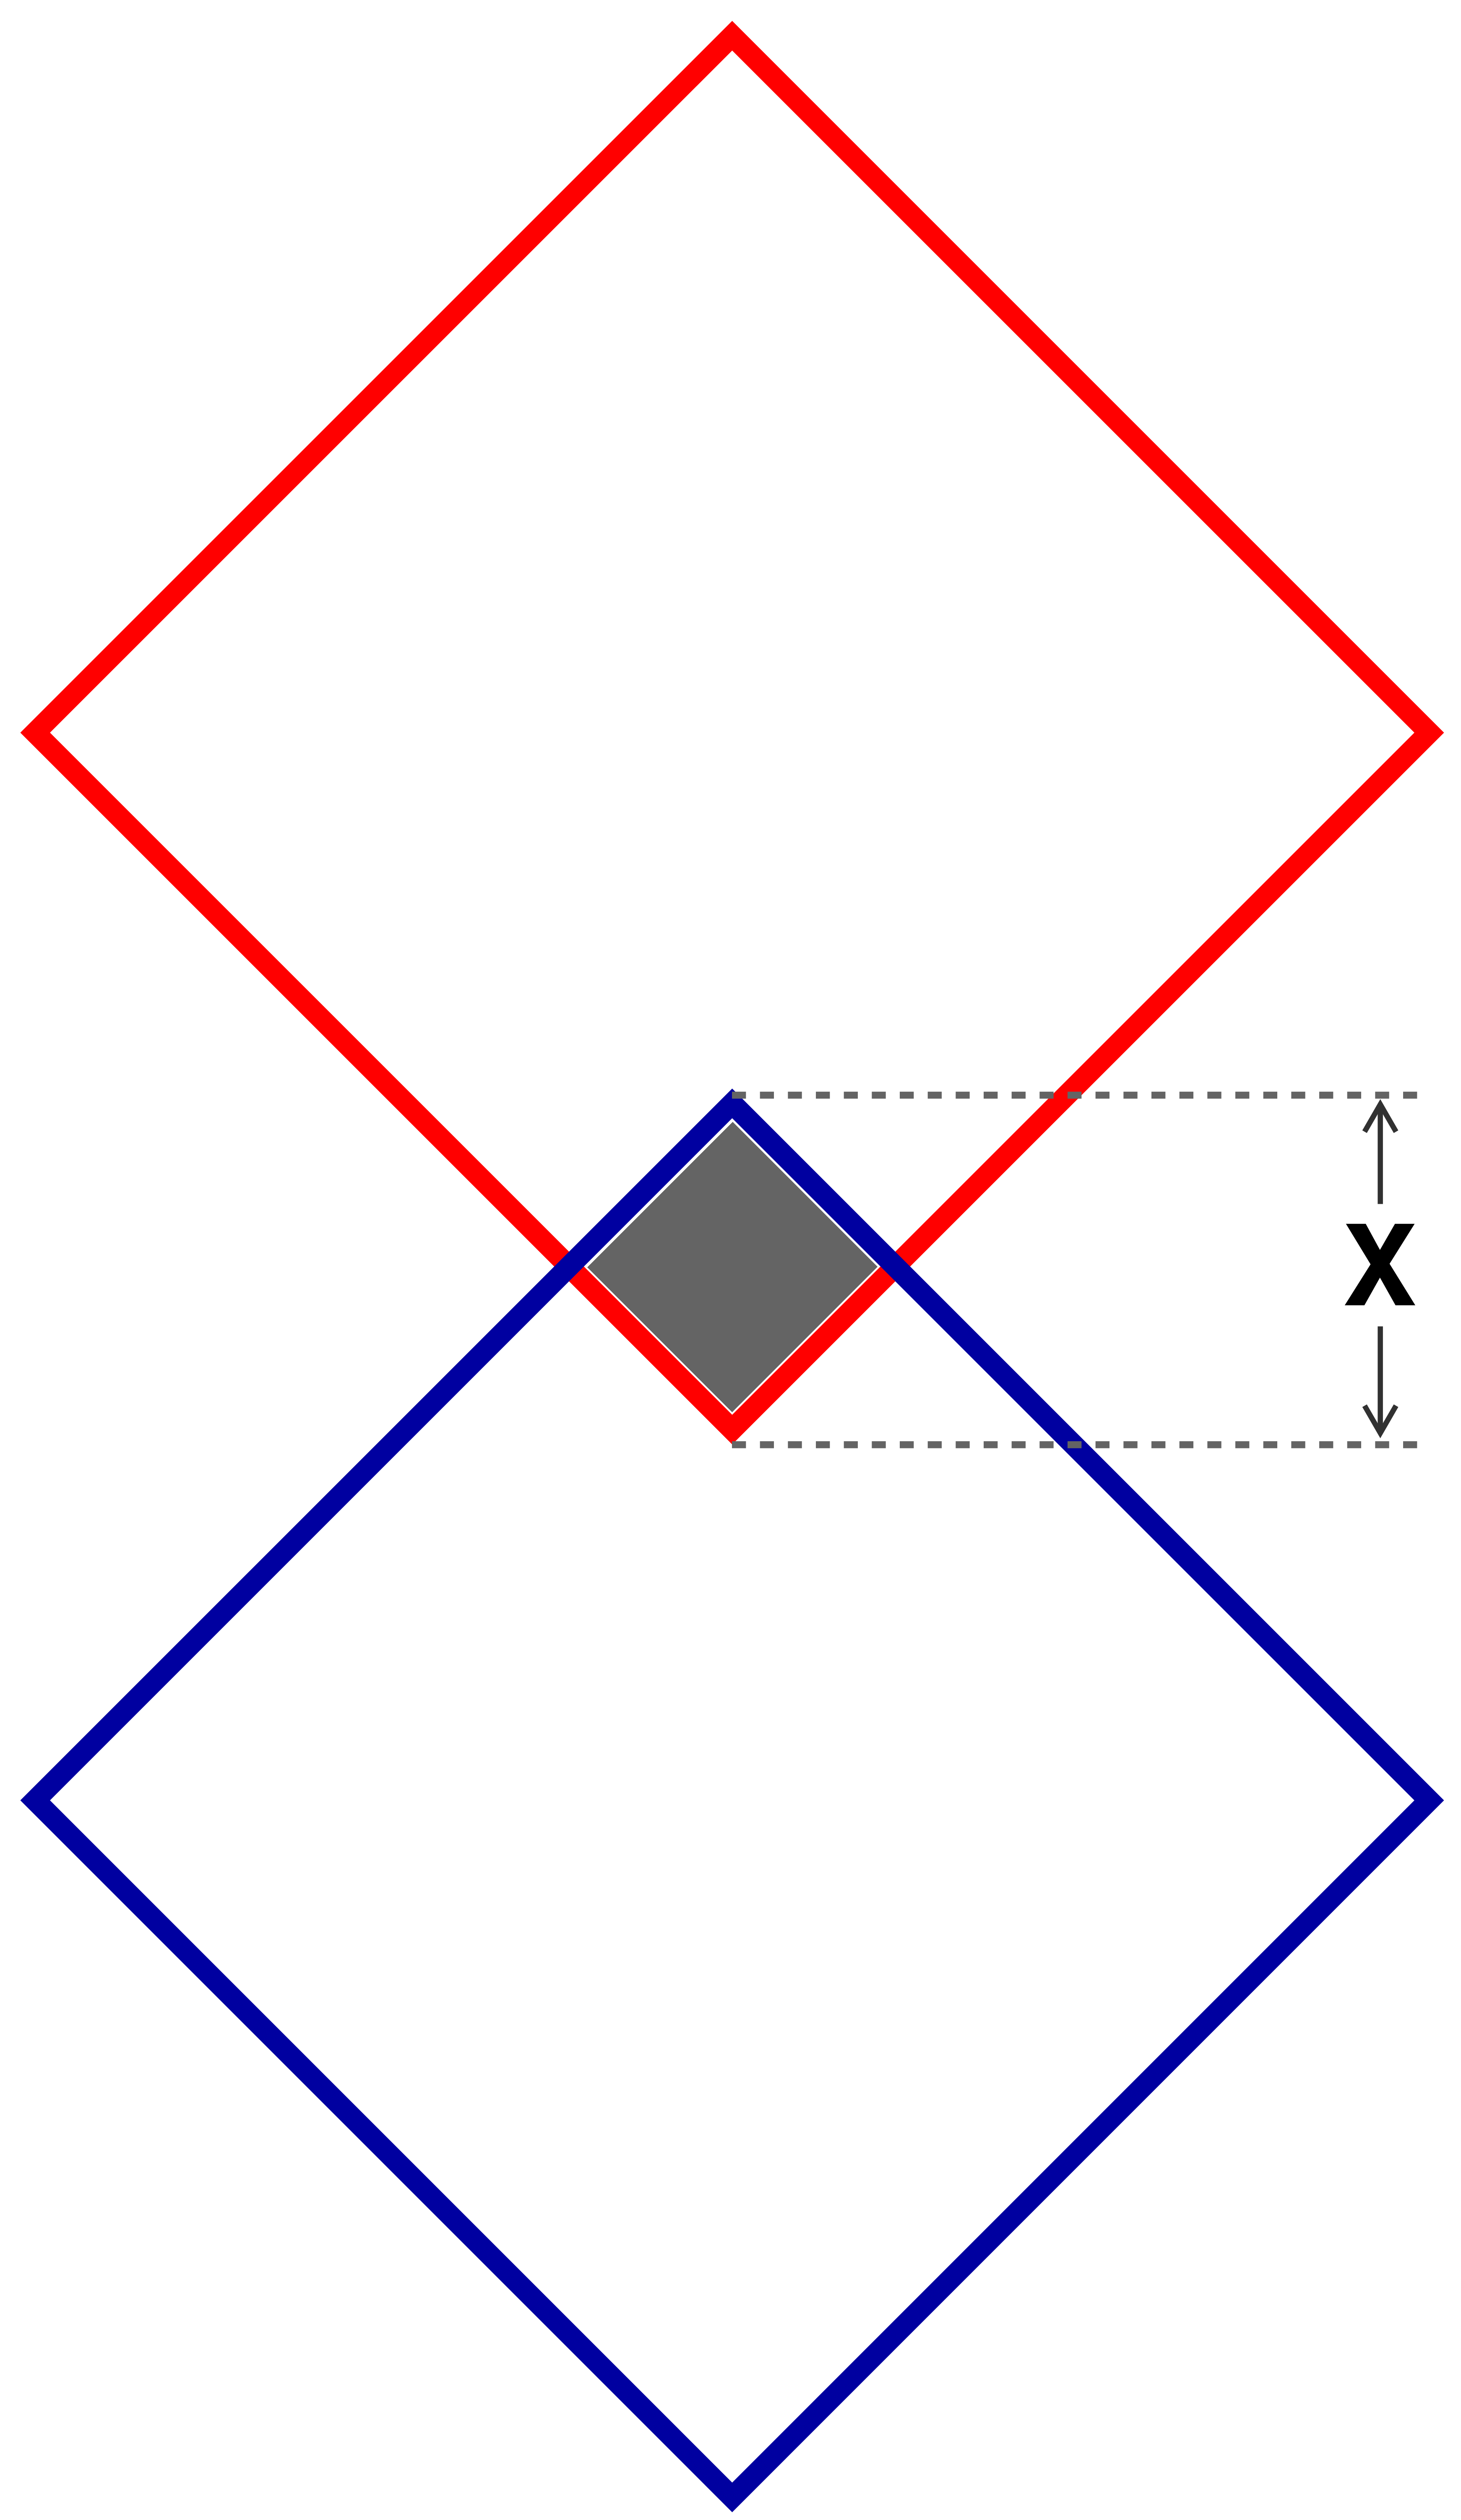
\includegraphics[height=2in]{orifice_app.png}
			\caption{Orifice geometry, repeated}
			\label{fig:orifice_rep}
		\end{figure}

		\begin{figure}[H]
			\centering
			
\includegraphics[height=2in]{orifice_detailed.png}
			\caption{Orifice geometry, detailed}
			\label{fig:orifice_detailed}
		\end{figure}

		The effective diameter of an orifice of any geometry is the diameter of a circle with equivalent area, such that
		
		\begin{equation}
			A = \frac{\pi}{4}D_{\text{effective}}^2
			\label{eq:d_eff}
		\end{equation}

		Thus, the height of the orifice X as defined in Figures~\ref{fig:orifice_rep} and \ref{fig:orifice_detailed}, which is directly driven by the actuator movement, 
		can be related to the effective diameter as follows:

		\begin{align}
			A &= \frac{\pi}{4}D_{\text{eff}}^2 = s^2 \\
			s &= \sqrt{\frac{\pi}{4}}D_{\text{eff}} \\
			X &= \sqrt{s^2 + s^2} = \sqrt{2}s \text{ by the Pythagorean Theorem}
		\end{align}

		Therefore,

			\begin{equation}
				X = \sqrt{2}\sqrt{\frac{\pi}{4}}D_{\text{eff}} = \sqrt{\frac{\pi}{2}}D_{\text{eff}}
			\end{equation}

		Finally, we can rearrange this relation to obtain the effective diameter as a function of X:

			\begin{equation}
				D_{eff} = \sqrt{\frac{2}{\pi}} X
			\end{equation}



\chapter{Required Relationship Failure Analysis}
\label{app:sat}

	Section~\ref{subsec:DFMEA::tol} introduces the most important failure consideration: satisfaction of the Required Relationship to the required tolerance as stipulated by Equation~\eqref{eq:required_relationship}:

	\begin{equation}
		\requiredRelationship
	\end{equation}

	The below analysis provides a thorough analysis of the effect of several key sources of error and analytically evaluates the final expected output of the \device.

	\section{Error Analysis}
	\label{app:sat:error}

		\subsection{Actuator Coefficient of Thermal Expansion}
		\label{app:sat:error:CTE}

			Typical material specifications list a single coefficient of thermal expansion (CTE).
			However, this value changes slightly as temperature changes, variation which must be accounted for where possible.
			NASA studied the behavior of aluminum across a wide temperature range and found its CTE as a function of temperature, presented in Figure~\ref{fig:al_alpha} \cite{ref_NASA_specs_Al}.
		
			\begin{figure}[H]
				\centering
				\fbox{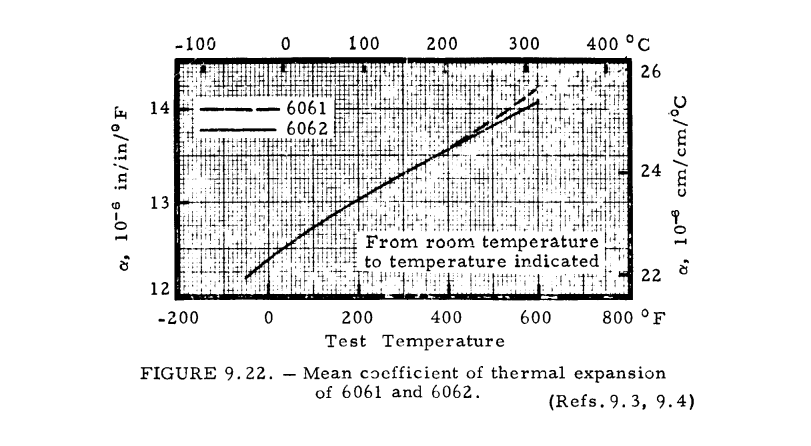
\includegraphics[width=0.8\textwidth]{Al_alpha_values}}
				\caption{Coefficient of thermal expansion of aluminum as a function of temperature}
				\label{fig:al_alpha}
			\end{figure}
			
			Though no numerical data was provided, the temperature-dependent aluminum CTE values can be approximated from this graph, shown in Table~\ref{tab:CTE_Al}.
			From this, we obtain the reference-temperature CTE (\specActuatorCTE) used in Chapter~\ref{chap:design},
			but the true value varies between \SI{21.8}{\micro\meter\per\meter\per\degreeCelsius} and \SI{23.5}{\micro\meter\per\meter\per\degreeCelsius} as $\Tcold \leq T \leq \Thot$.
			These introduce nonlinear behavior, resulting in quantifiable error.

		\subsection{Machine Tolerances}
		\label{app:sat:error:mach}

			\begin{wrapfigure}{l}{.4\textwidth}
				\centering
				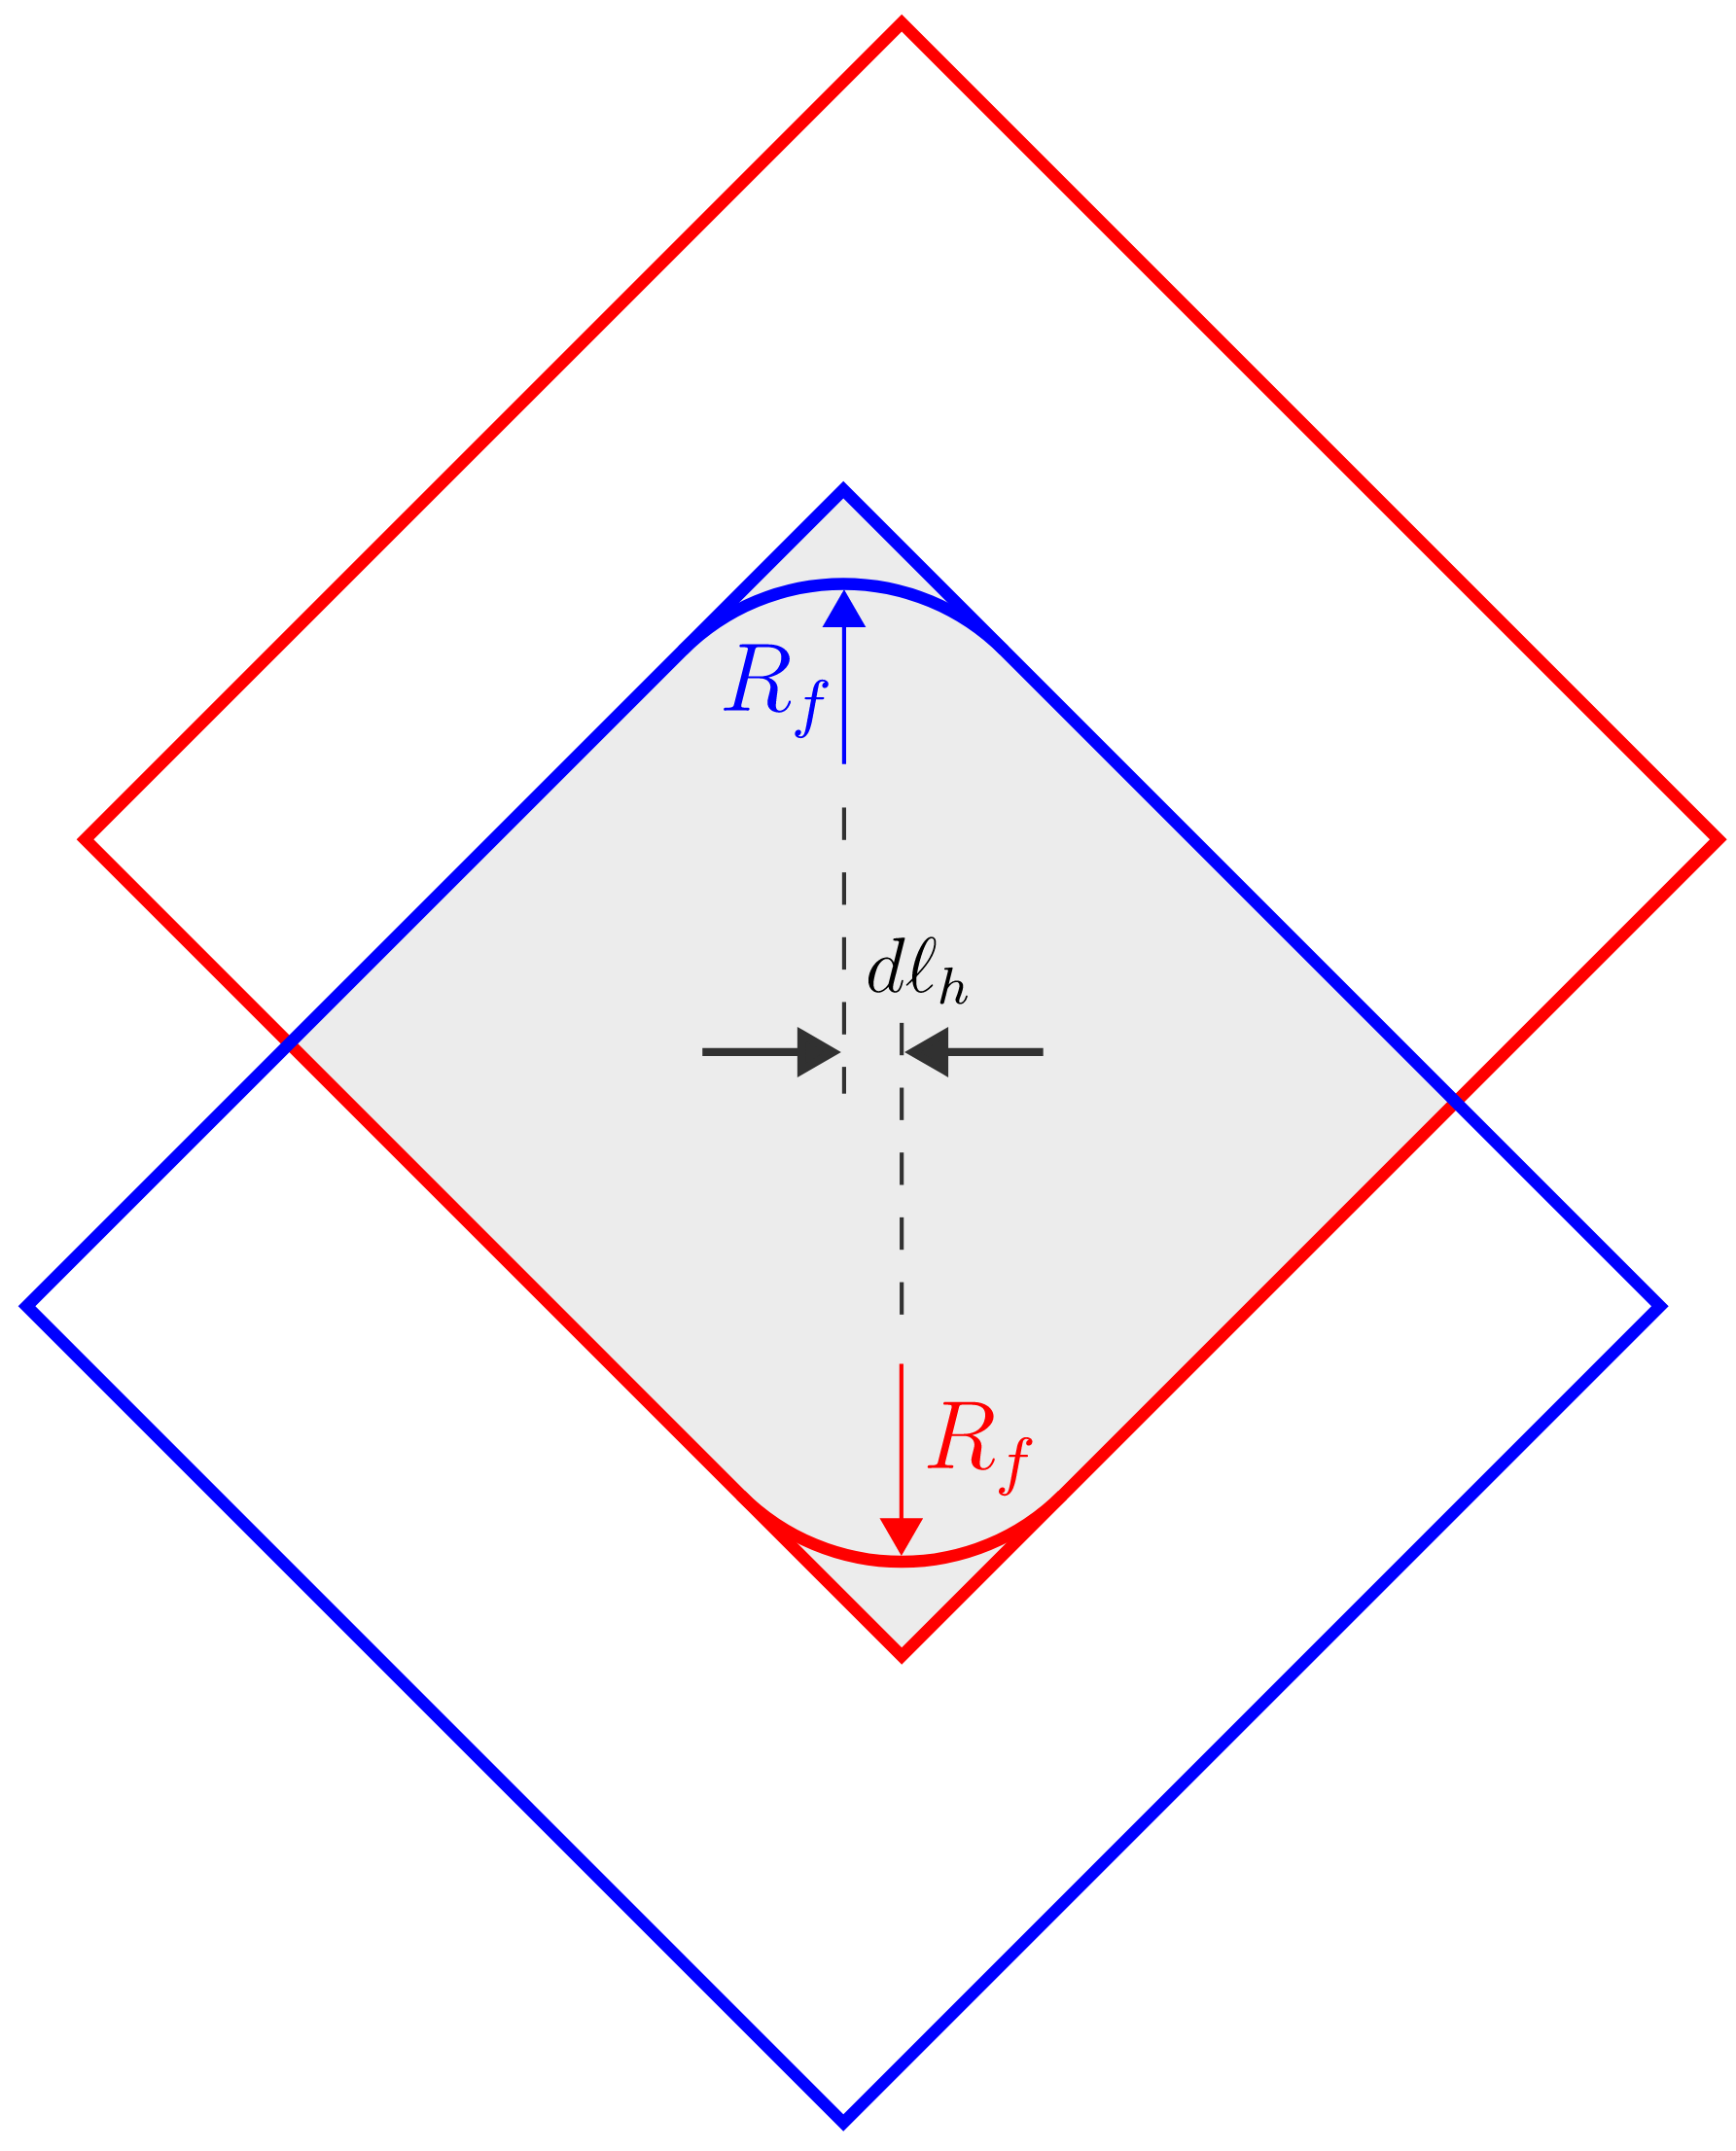
\includegraphics[width=.39\textwidth]{orif_error.png}
				\caption{Orifice error modes}
				\label{fig:orif_error}
			\end{wrapfigure}

			General machine dimension tolerances depend on the capabilities of the manufacturing devices available.
			It is reasonable to assume that Sandia's tolerance capabilities meet or exceed those of standard Computer-Numerical Control (CNC) mills.
			The values represented in the engineering drawings (Appendix~\ref{app:drawings}) are taken from HAAS VF-2 series specifications \cite{ref_haas}.

			The two square holes that make the orifice will be machined with Wire EDM. Two critical tolerances significantly influence the effective diameter of the orifice:
			the horizontal position of each hole and the fillet radii at the top and bottom vertices. The side vertices are made by the intersection of two straight cuts and can be assumed to be sharp.
			Figure~\ref{fig:orif_error} depicts these two error modes. Milco Wire EDM, Inc quoted the operation (attached in Appendix~\ref{app:datasheets}).
			They can achieve a minimum fillet radius $R_f = \SI{76.2}{\micro\meter}$ and horizontally position each orifice to a tolerance of \SI{12.7}{\micro\meter}.
			This horizontal error compounds if the leading orifice is machined too far left and the trailing orifice is machined too far right;
			the maximum error is twice this value. Thus, $d \ell_h = \SI{25.4}{\micro\meter}$.
			Vertical error can be more readily dealt with individually; thus, the noncompounding vertical error is defined as $d \ell_v = \SI{12.7}{\micro\meter}$.

		\subsection{Bellows Spring Reactions}
		\label{app:sat:error:bellows}

			As the actuator deflects and drives the valve stem downwards or pulls it upwards, the two bellows act as springs and provide a slight reaction force, possibly compressing or stretching the valve stem and actuator.
			Since each part behaves as a spring, the resulting coupled spring assembly is complex and requires a comprehensive force balance analysis to reconcile the final deflections.

		Other sources of error include unwanted thermal expansion of the housing and valve subcomponents and potential heat transfer from the hot internal gas.
		Each of these sources of error impacts the entire system. Since the behavior of each subsystem is coupled, the effect of these errors on the final output of the \device\ can only be analyzed by a rigorous static system analysis.
		As discussed in Section~\ref{subsec:DFMEA::tol}, the transfer function derived in the following section provides a tool for analysis of deterministic and stochastic error propagation across the full temperature range.

	\section{Transfer Function Derivation}
	\label{app:sat:TF}

		The required transfer function from Section~\ref{subsec:intro:specs:RR} describes the system under ideal conditions and cannot properly account for systematic errors.
		To fully analyze the expected performance of the \device, a new, comprehensive system Transfer Function must be derived that can be compared to the required output: 

		\begin{equation}
			\hat{G}_{sys} = A_1 (T-T_{ref}) + A_0 = (\Aone)(T-T_{ref}) + (\Azero)
			\label{eq:req_TF}
		\end{equation}

		This section presents a full derivation of this transfer function, represented in block-diagram form on the following page:
		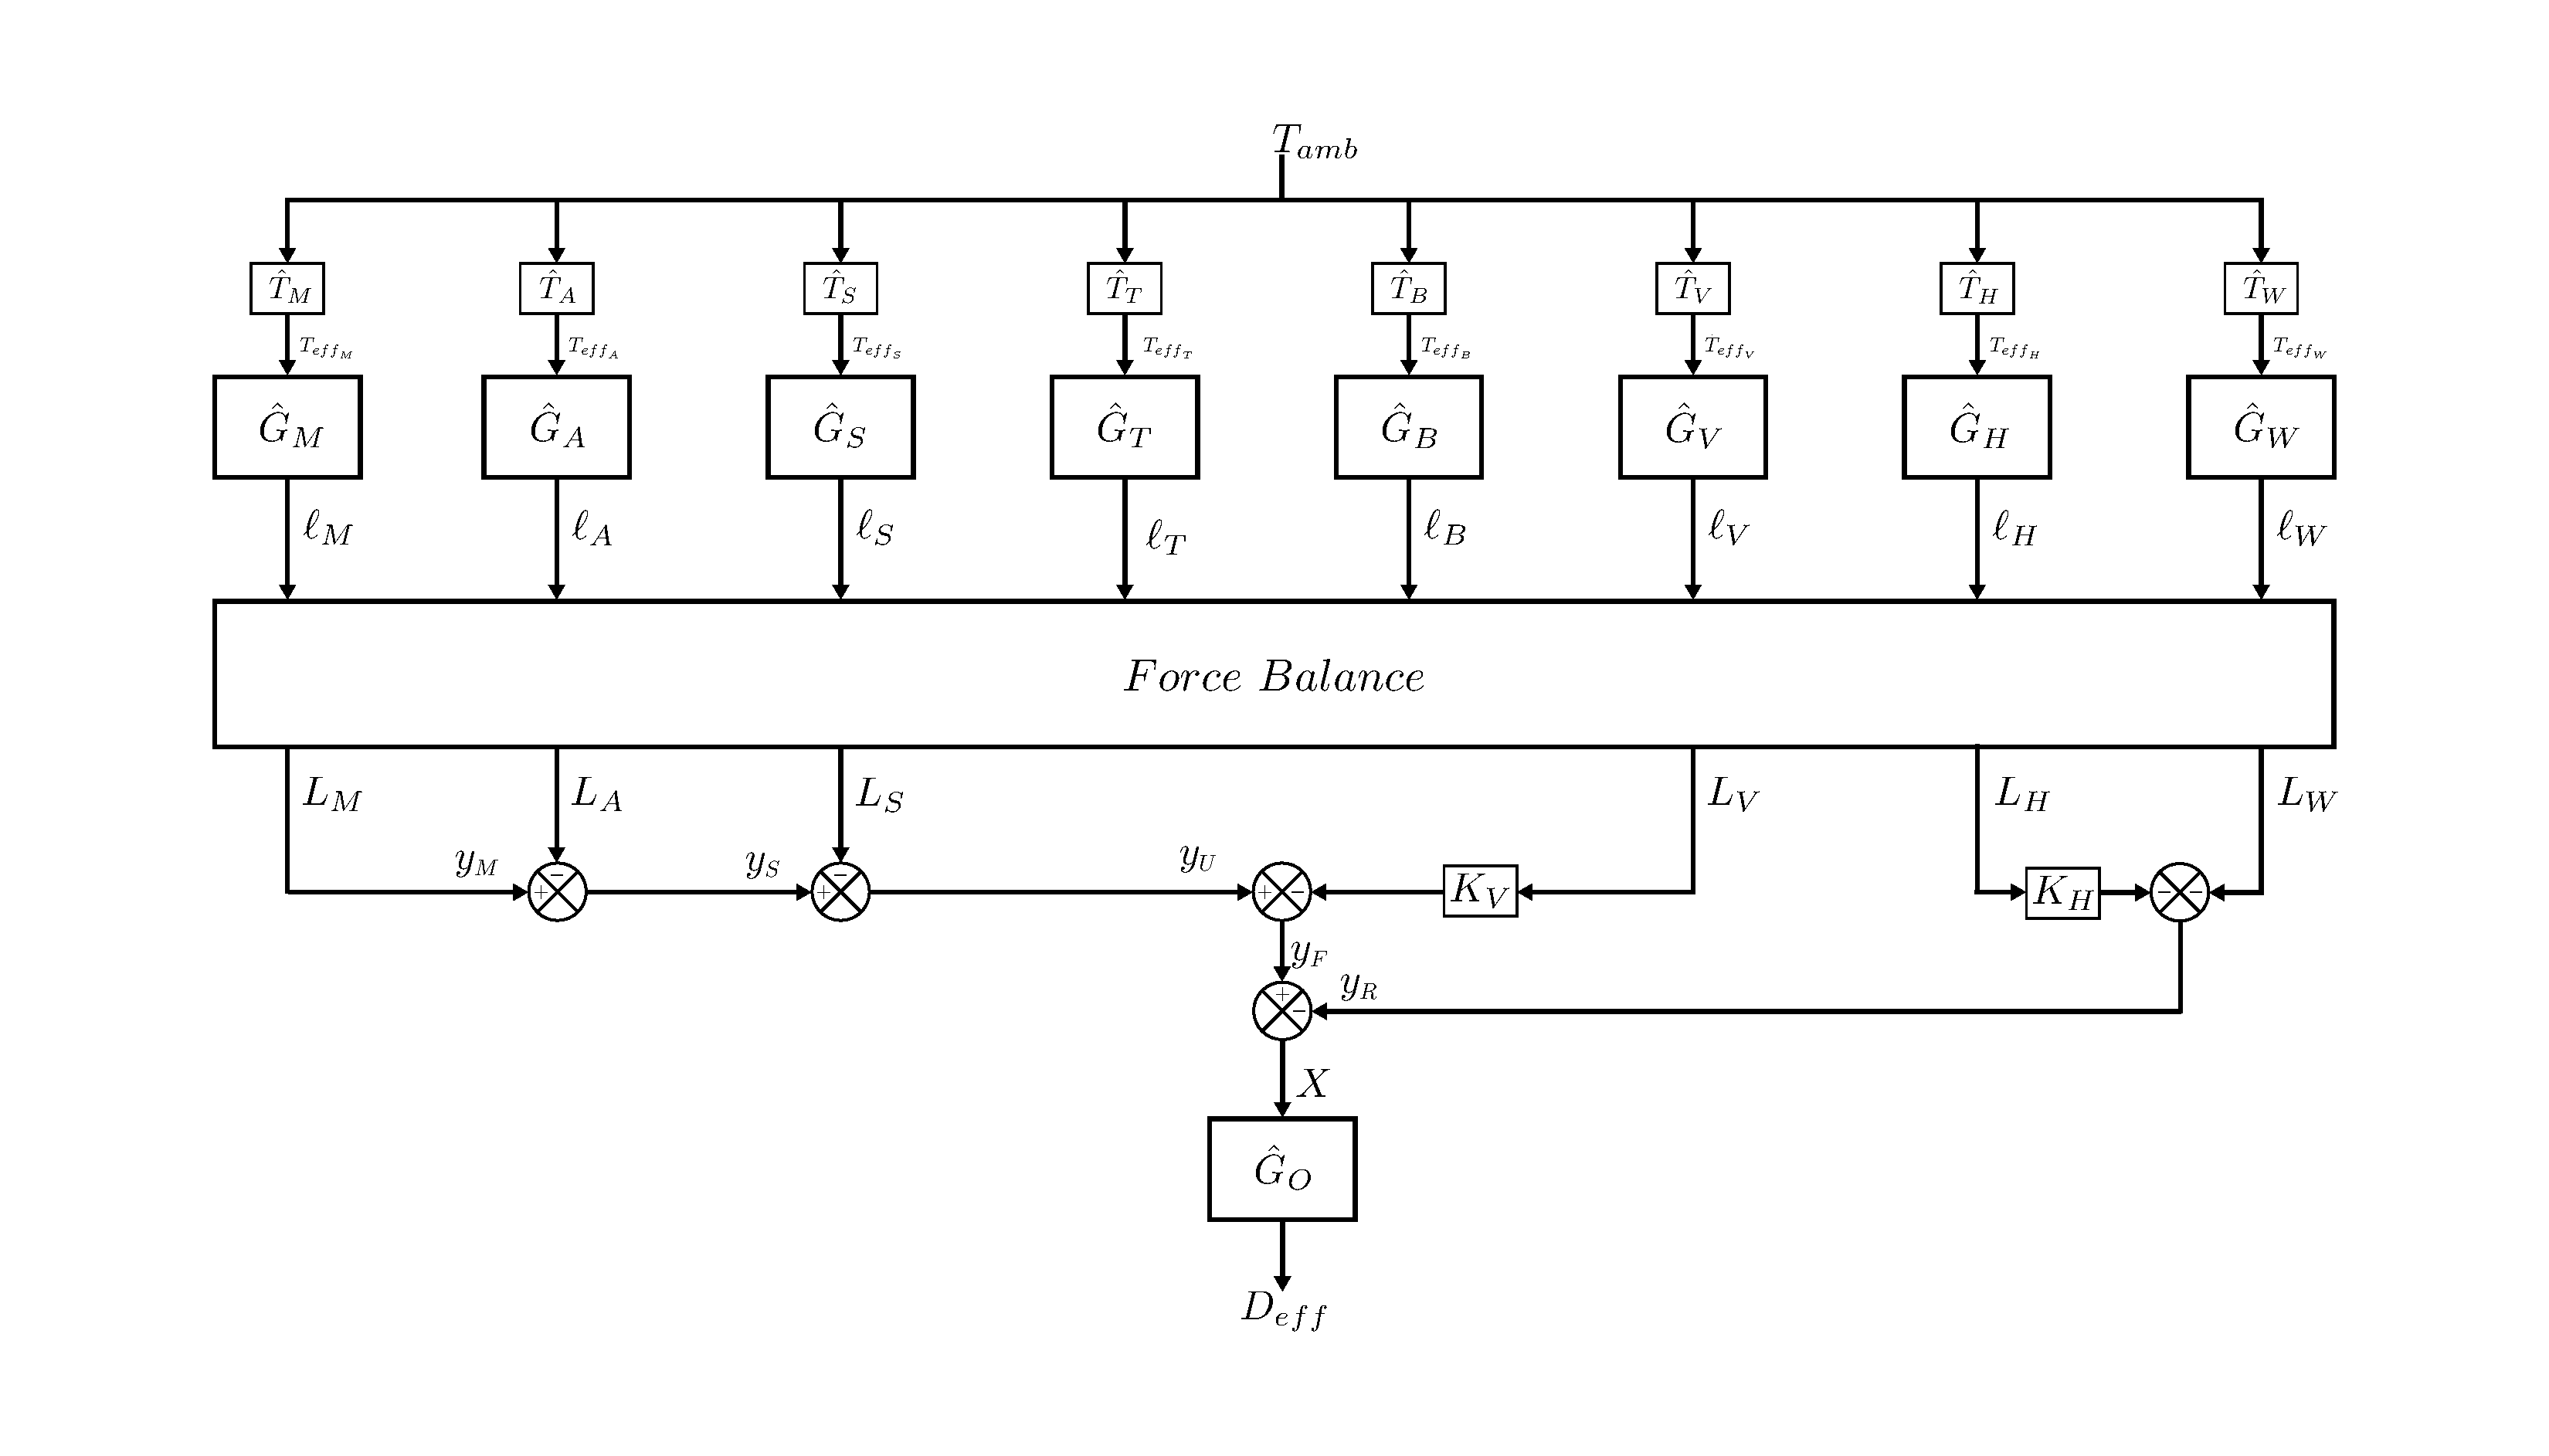
\includepdf[pages=1, fitpaper=true, landscape=true]{pdf/TF_import.pdf}

		The \device\ System Transfer Function comprises 21 smaller independent transfer functions whose respective output values are summed and equated in accordance with the physical behavior of the system.
		Its details will take a moment to unpack.

		First, notice the general structure: the transfer function receives $T_{ambient}$ and returns $D_{effective}$ as prescribed.
		The smaller, top $(\hat{T})$ row of sub-transfer functions adjusts $T_{amb}$ for each part in the assembly to account for heat transfer from the hot internal gas.
		The larger, second $(\hat{G})$ row represents the thermal expansion of each dimensionally critical component; each function takes the given adjusted temperature and outputs the thermally expanded length $\ell$ of its respective part.
		However, because the bellows apply a spring force against the actuation motion, these parts will deform slightly. A Force Balance processes these undeformed length values through a system of linear equations, yielding the final length $L$ of each component.
		These final values are summed to obtain the position $y$ of each of the two square holes. Taking the difference between these positions, we obtain the height $X$ of the square orifice, which is finally converted to $D_{effective}$ by the orifice transfer function $\hat{G}_O$.
		
		To understand the origin of the transfer function structure, we must decompose the functional structure of each component of the \device.
		Figure~\ref{fig:positional_block_diagram} illustrates the relative position of each component in simplified fashion.
		Each part's temperature adjustment function $\hat{T}$, thermal transfer function $\hat{G}$, undeformed length $\ell$, and final length $L$ is labeled with its respective subscript as shown in the figure:
		
		\begin{multicols}{2}
			\begin{itemize}
				\item Mount (M)
				\item Actuator (A)
				\item Upper valve stem (S)
				\item Upper ``top'' bellows (T)
				\item Lower ``bottom'' bellows (B)
				\item Valve orifice (V)
				\item Housing side walls (H)
				\item Housing top face or ``wall'' (W)
			\end{itemize}
		\end{multicols}

		The positional block diagram defines how each part is coupled to the others, enabling the force balance required to find the spring deflection of each flexible part.
		The labeled heights move as each part expands or contracts, yielding the final position of each orifice as the net sum of the stretched and compressed parts.
				
		\begin{figure}[H]
			\centering
			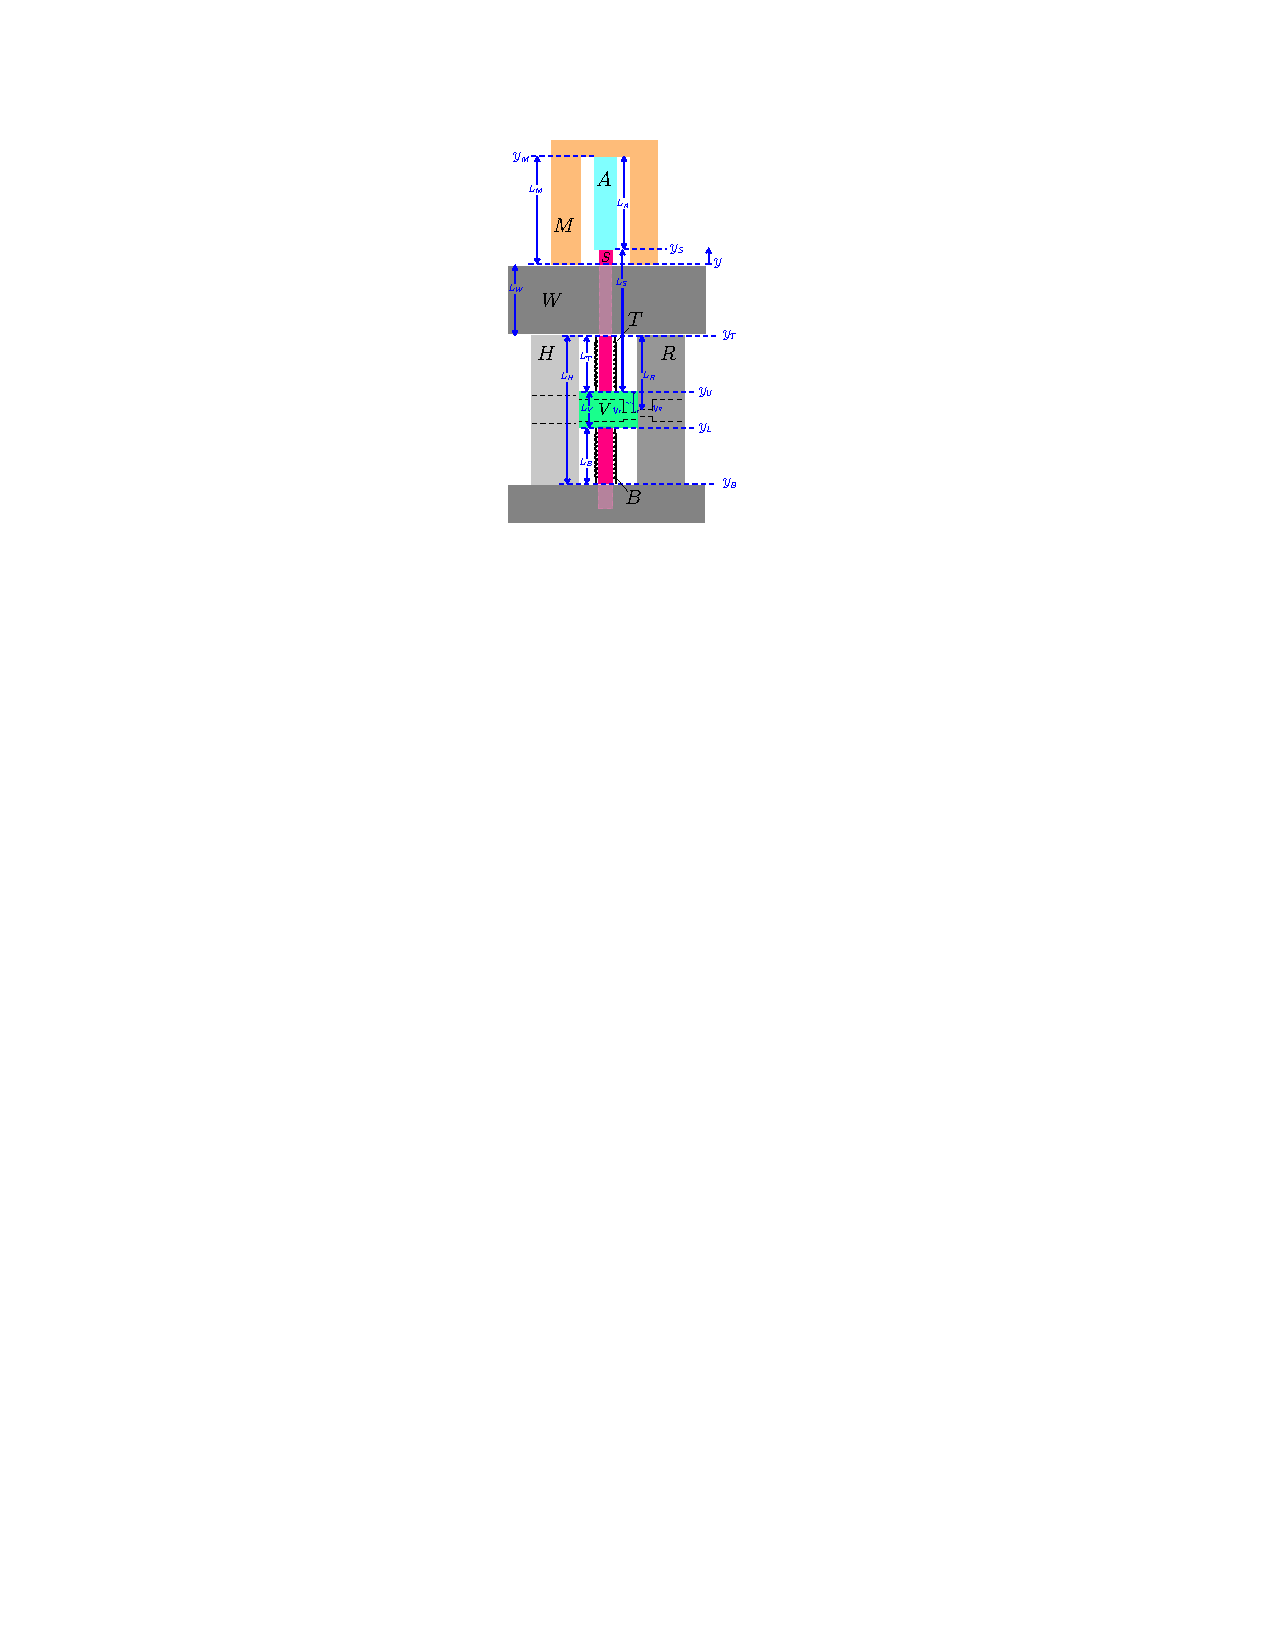
\includegraphics[height=.98\textheight, width=\textwidth, keepaspectratio]{positional_block_diagram.png}
			\caption{Positional block diagram}
			\label{fig:positional_block_diagram}
		\end{figure}
		
		
		\begin{multicols}{2}
			\begin{figure}[H]
				\centering
				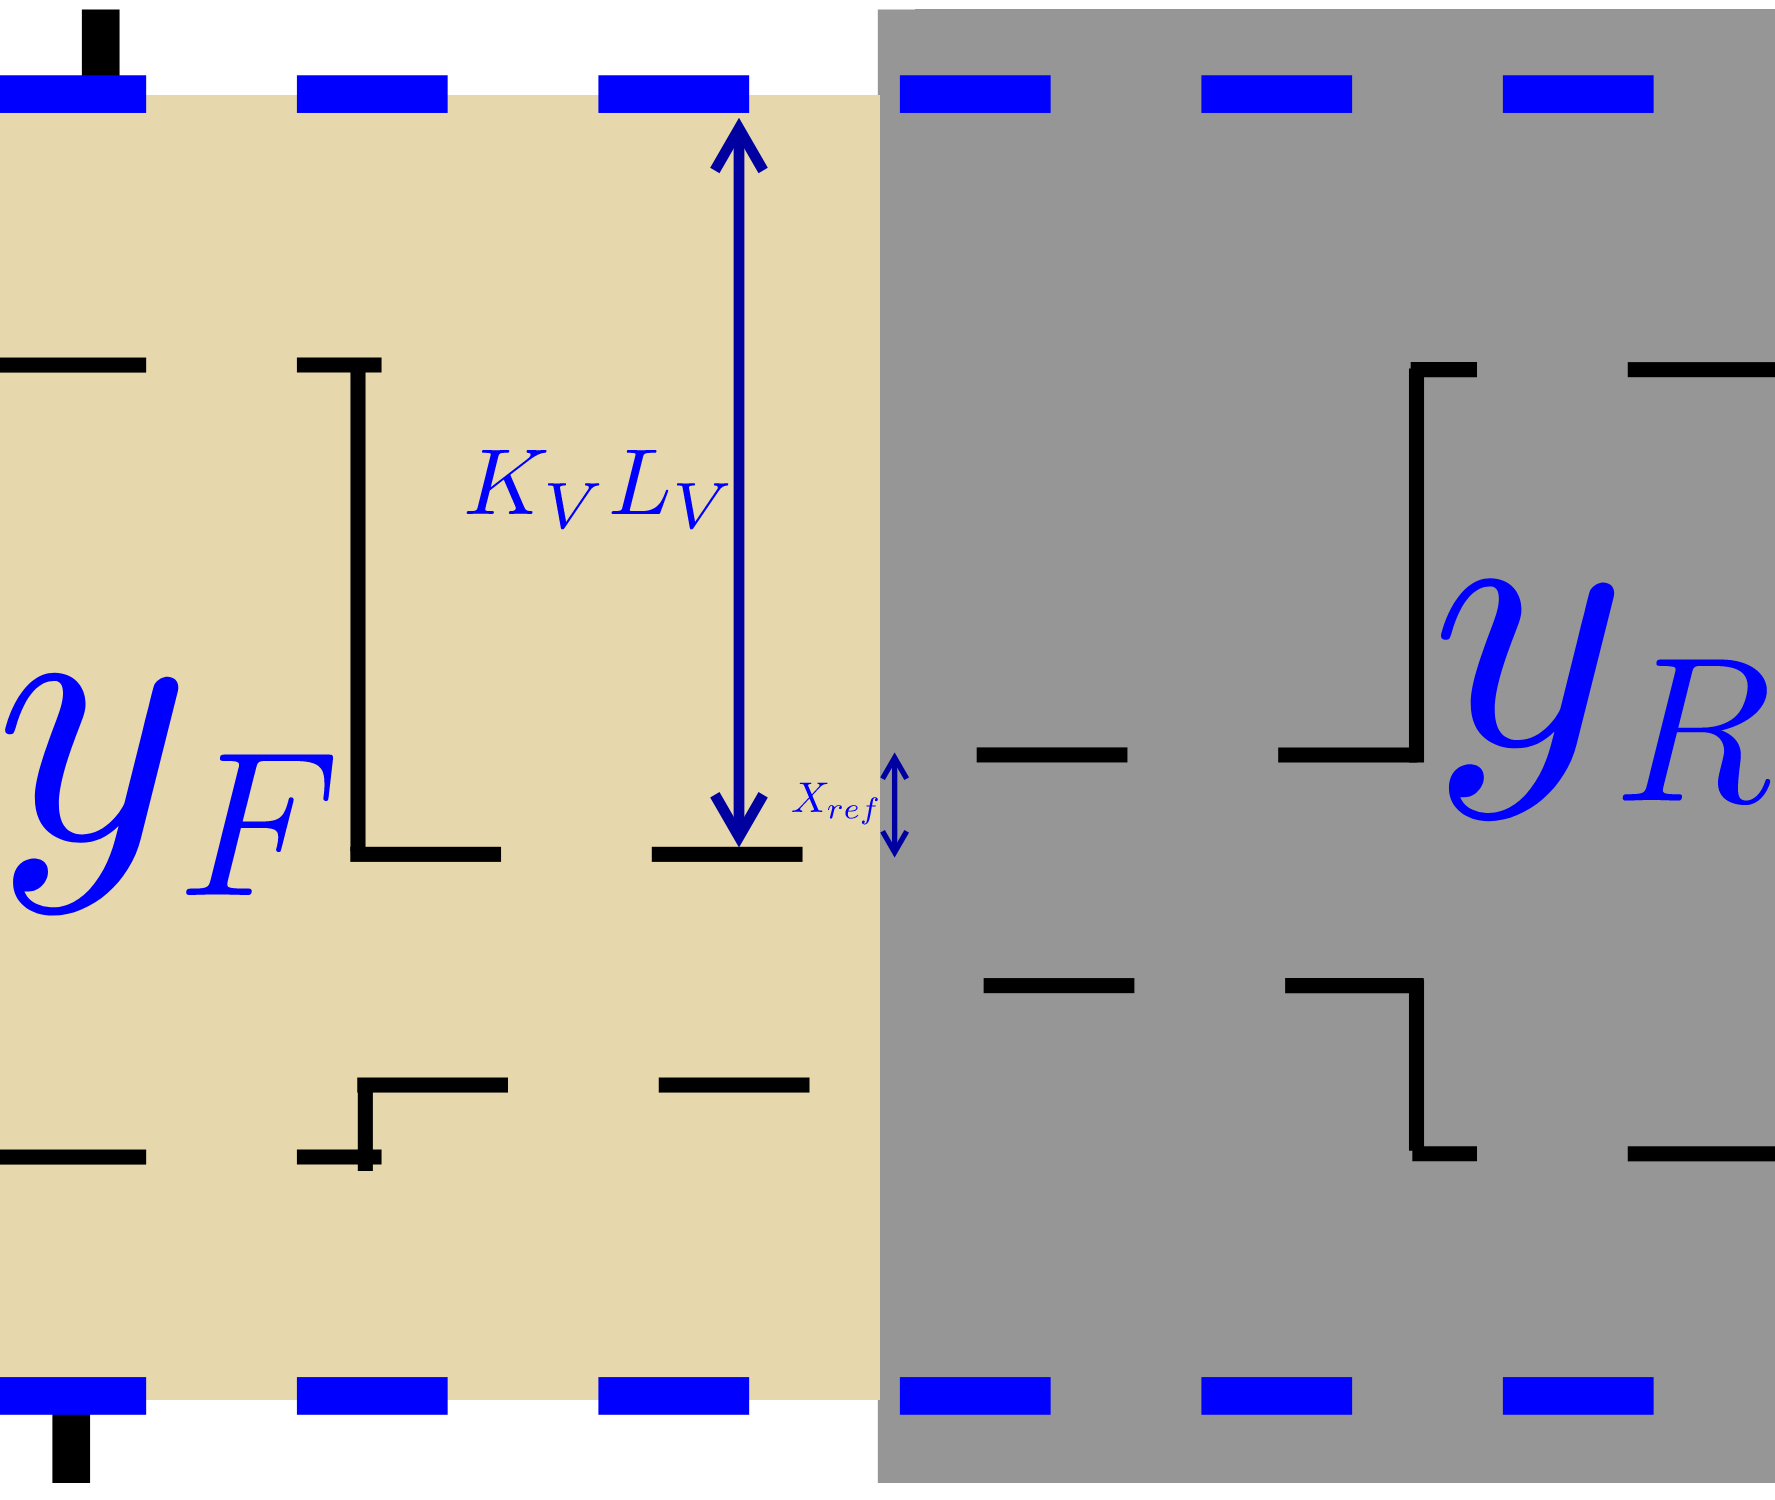
\includegraphics[width=.45\textwidth]{positional_block_diagram_zoom.png}
				\caption{Positional block diagram, detail view}
				\label{fig:positional_block_diagram_zoom}
			\end{figure}

			\begin{figure}[H]
				\centering
				\includegraphics[width=.45\textwidth]{Housing_split.png}
				\caption{Separation between Housing Wall (W) and Housing Body (H)}
				\label{fig:housing_split}
			\end{figure}

			\columnbreak
			
			Figure~\ref{fig:positional_block_diagram_zoom} shows a detail view of certain dimensions around the orifice that will be used later.
			As described in Chapter~\ref{chap:design}, the mount $(M)$ sits atop the housing.
			The actuator $(A)$ dangles from the upper interior surface of the housing center, which for our purposes is defined as the undersurface of the belleville washer.
			The upper valve stem $(S)$ hangs from the bottom of the actuator, passes through the housing wall, and suspends the valve orifice $(V)$, which slides freely against the two surfaces $H$ and $R$.
			Treating the three housing components as a single part, which is realistic because they are Electron Beam welded at every seam, the housing ``wall'' $(W)$ is defined as the top \SI{10}{\milli\meter} of the whole housing assembly (parts V1, V2, and V3) as shown in Figure~\ref{fig:housing_split}.
			The housing body $(H)$ and ``rear'' $(R)$ share the lower portion shown in the figure; their expansion is coupled.
			These represent the side walls of the housing and behave identically; thus, their behavior is summed by the $H$ term in several calculations.
			The two bellows $(T \text{ and } B)$ span the distance between the valve orifice and the upper and lower housing walls (part V2).
			
			Figure~\ref{fig:positional_block_diagram} also defines several useful positions according to a vertical coordinate frame. The position variable $y$ originates (i.e. equals $0$) at the top surface of the housing, which is considered fixed, and increases vertically.
			Thus, $y_M$ is positive, whereas $y_T$ is negative.
		\end{multicols}

		\subsection{Heat Transfer}
		\label{app:sat:TF:dT}

			The very top row evaluates the final effective temperature of each part assuming a worst-case thermal gradient driven by a \SI{20}{\degreeCelsius} temperature difference between the internal gas
			and the ambient temperature. The temperature of every wetted part is set to the gas temperature. The actuator and mount temperatures are assumed to follow $T_{amb}$ exactly, but the tools for a more complex
			heat transfer analysis between the subsystems were developed in Chapter~\ref{chap:test}, providing a starting ground to determine the final steady-state temperature of the actuator.
			The results presented in this Appendix, however, do not properly reflect this heat transfer and simply show the output of the \device\ for gas that follows the ambient temperature.
		
		\subsection{Thermal Expansion}
		\label{app:sat:TF:G_therm}

			Let us forgo the top row of temperature-adjusting functions for now and assume we know the temperature of each part. A full thermal analysis will provide these values later in this report.
			Each of the eight sub-transfer functions along the second row computes the thermal expansion of each part shown in Figure~\ref{fig:positional_block_diagram}.
			Its value can be approximated as a first-order Taylor Expansion\cite{ref_Jensen, ref_Stewart} with very little error due to the linear behavior of thermal expansion. This yields

				\begin{equation}
					\ell_i = \hat{G}_{thermal} = \ell_0(1 + \frac{d \ell}{dT} \Delta T)
				\end{equation}

			where $\hat{G}_{thermal}$ outputs the expanded dimension $\ell_i$ of part $i$, $\ell_0$ is its machined dimension, and $\Delta T = (T_{amb} - T_{ref})$.
			According to the general principle of thermal expansion\cite[Eq.~4-4]{ref_Hibbeler}, $\frac{d \ell}{dT} = \alpha \ell_0$ where $\alpha$ is the material Coefficient of Thermal Expansion (CTE).
			Thus, the thermal-expansion transfer functions are defined as follows:

			\begin{align}
					\hat{G}_M &= \ell_{M_0} (1 + \alpha_{ALLV} ( T_{{eff}_M} - T_{ref} ) ) &
					\hat{G}_B &= \ell_{B_0} (1 + \alpha_{Inc} ( T_{{eff}_B} - T_{ref} ) ) \label{eq:G_therm_1}\\
					\hat{G}_A &= \ell_{A_0} (1 + \alpha_{Al} ( T_{{eff}_A} - T_{ref} ) ) &
					\hat{G}_V &= \ell_{V_0} (1 + \alpha_{Inv} ( T_{{eff}_V} - T_{ref} ) ) \\
					\hat{G}_S &= \ell_{S_0} (1 + \alpha_{Inv} ( T_{{eff}_S} - T_{ref} ) ) &
					\hat{G}_H &= \ell_{H_0} (1 + \alpha_{Inv} ( T_{{eff}_H} - T_{ref} ) ) \\
					\hat{G}_T &= \ell_{T_0} (1 + \alpha_{Inc} ( T_{{eff}_T} - T_{ref} ) ) &
					\hat{G}_W &= \ell_{W_0} (1 + \alpha_{Inv} ( T_{{eff}_W} - T_{ref} ) ) \label{eq:G_therm_last}
			\end{align}

			where the material expansion coefficients and machined lengths are as follows.

			Material coefficients of thermal expansion:

			\begin{itemize}
				\item Aluminum (Al): \specActuatorCTE\cite[Table~9-22]{ref_NASA_specs_Al}
				\item ALLVAR (ALLV): \specMountCTE\cite{ref_AllvarAlloys}
				\item Invar 36 (Inv): \specInvarCTE\cite{ref_Carpenter_Inv}
				\item Inconel 718 (Inc): \specInconelCTE\cite{ref_SpecialMetals_Inc}
			\end{itemize}

			and the machined dimensions $\ell_{i_0}$ from Appendix~\ref{app:drawings}:

			\begin{itemize}
				\item $\ell_{M_0} = \SI{38.541}{\milli\meter} - \SI{0.55}{\milli\meter} = \SI{38.041}{\milli\meter}$\footnote{Top of the mount, for simplicity, is assumed to be the underside of the compressed belleville washer. Since this height is dependent on the use case, we will assume a \SI{0.05}{\milli\meter} compression.}
				\item $\ell_{A_0} = \SI{32.991}{\milli\meter}$
				\item $\ell_{S_0} = \SI{70.72}{\milli\meter} - \SI{32.86}{\milli\meter} = \SI{37.86}{\milli\meter}$
				\item $\ell_{T_0} = \SI{22.86}{\milli\meter}$
				\item $\ell_{B_0} = \ell_{T_0} = \SI{22.86}{\milli\meter}$
				\item $\ell_{V_0} = \SI{32.86}{\milli\meter} - \SI{27.86}{\milli\meter} = \SI{5}{\milli\meter}$
				\item $\ell_{H_0} = \SI{63.72}{\milli\meter}$
				\item $\ell_{W_0} = \SI{10}{\milli\meter}$
			\end{itemize}

			This yields eight undeformed lengths, helping us to define the positions of each part of the orifice.
			The CTE of aluminum is computed as a function of temperature as defined in Section~\ref{app:sat:error:CTE} to find the impact of this error on the final output.
			Dimensional errors are stochastically added or subtracted to each machined part length $\ell_0$. This process is discussed in more detail in Section~\ref{app:sat:TF:results}. 
			Before this can be calculated, however, the spring reaction of bellows must be reconciled.

		\subsection{Force Balance}
		\label{app:sat:TF:force_balance}

			Each component is undeformed at the machining and assembly temperature, $T_{ref}$. Thus, $L_i(T_{ref}) = \ell_i(T_{ref})$.
			As the temperature changes and the connected parts expand at different rates, the system behaves as a static coupled spring mechanism. The arrangement is shown in Figure~\ref{fig:springs}.

			\begin{figure}[H]
				\centering
				\begin{minipage}{.45\textwidth}
					\centering
					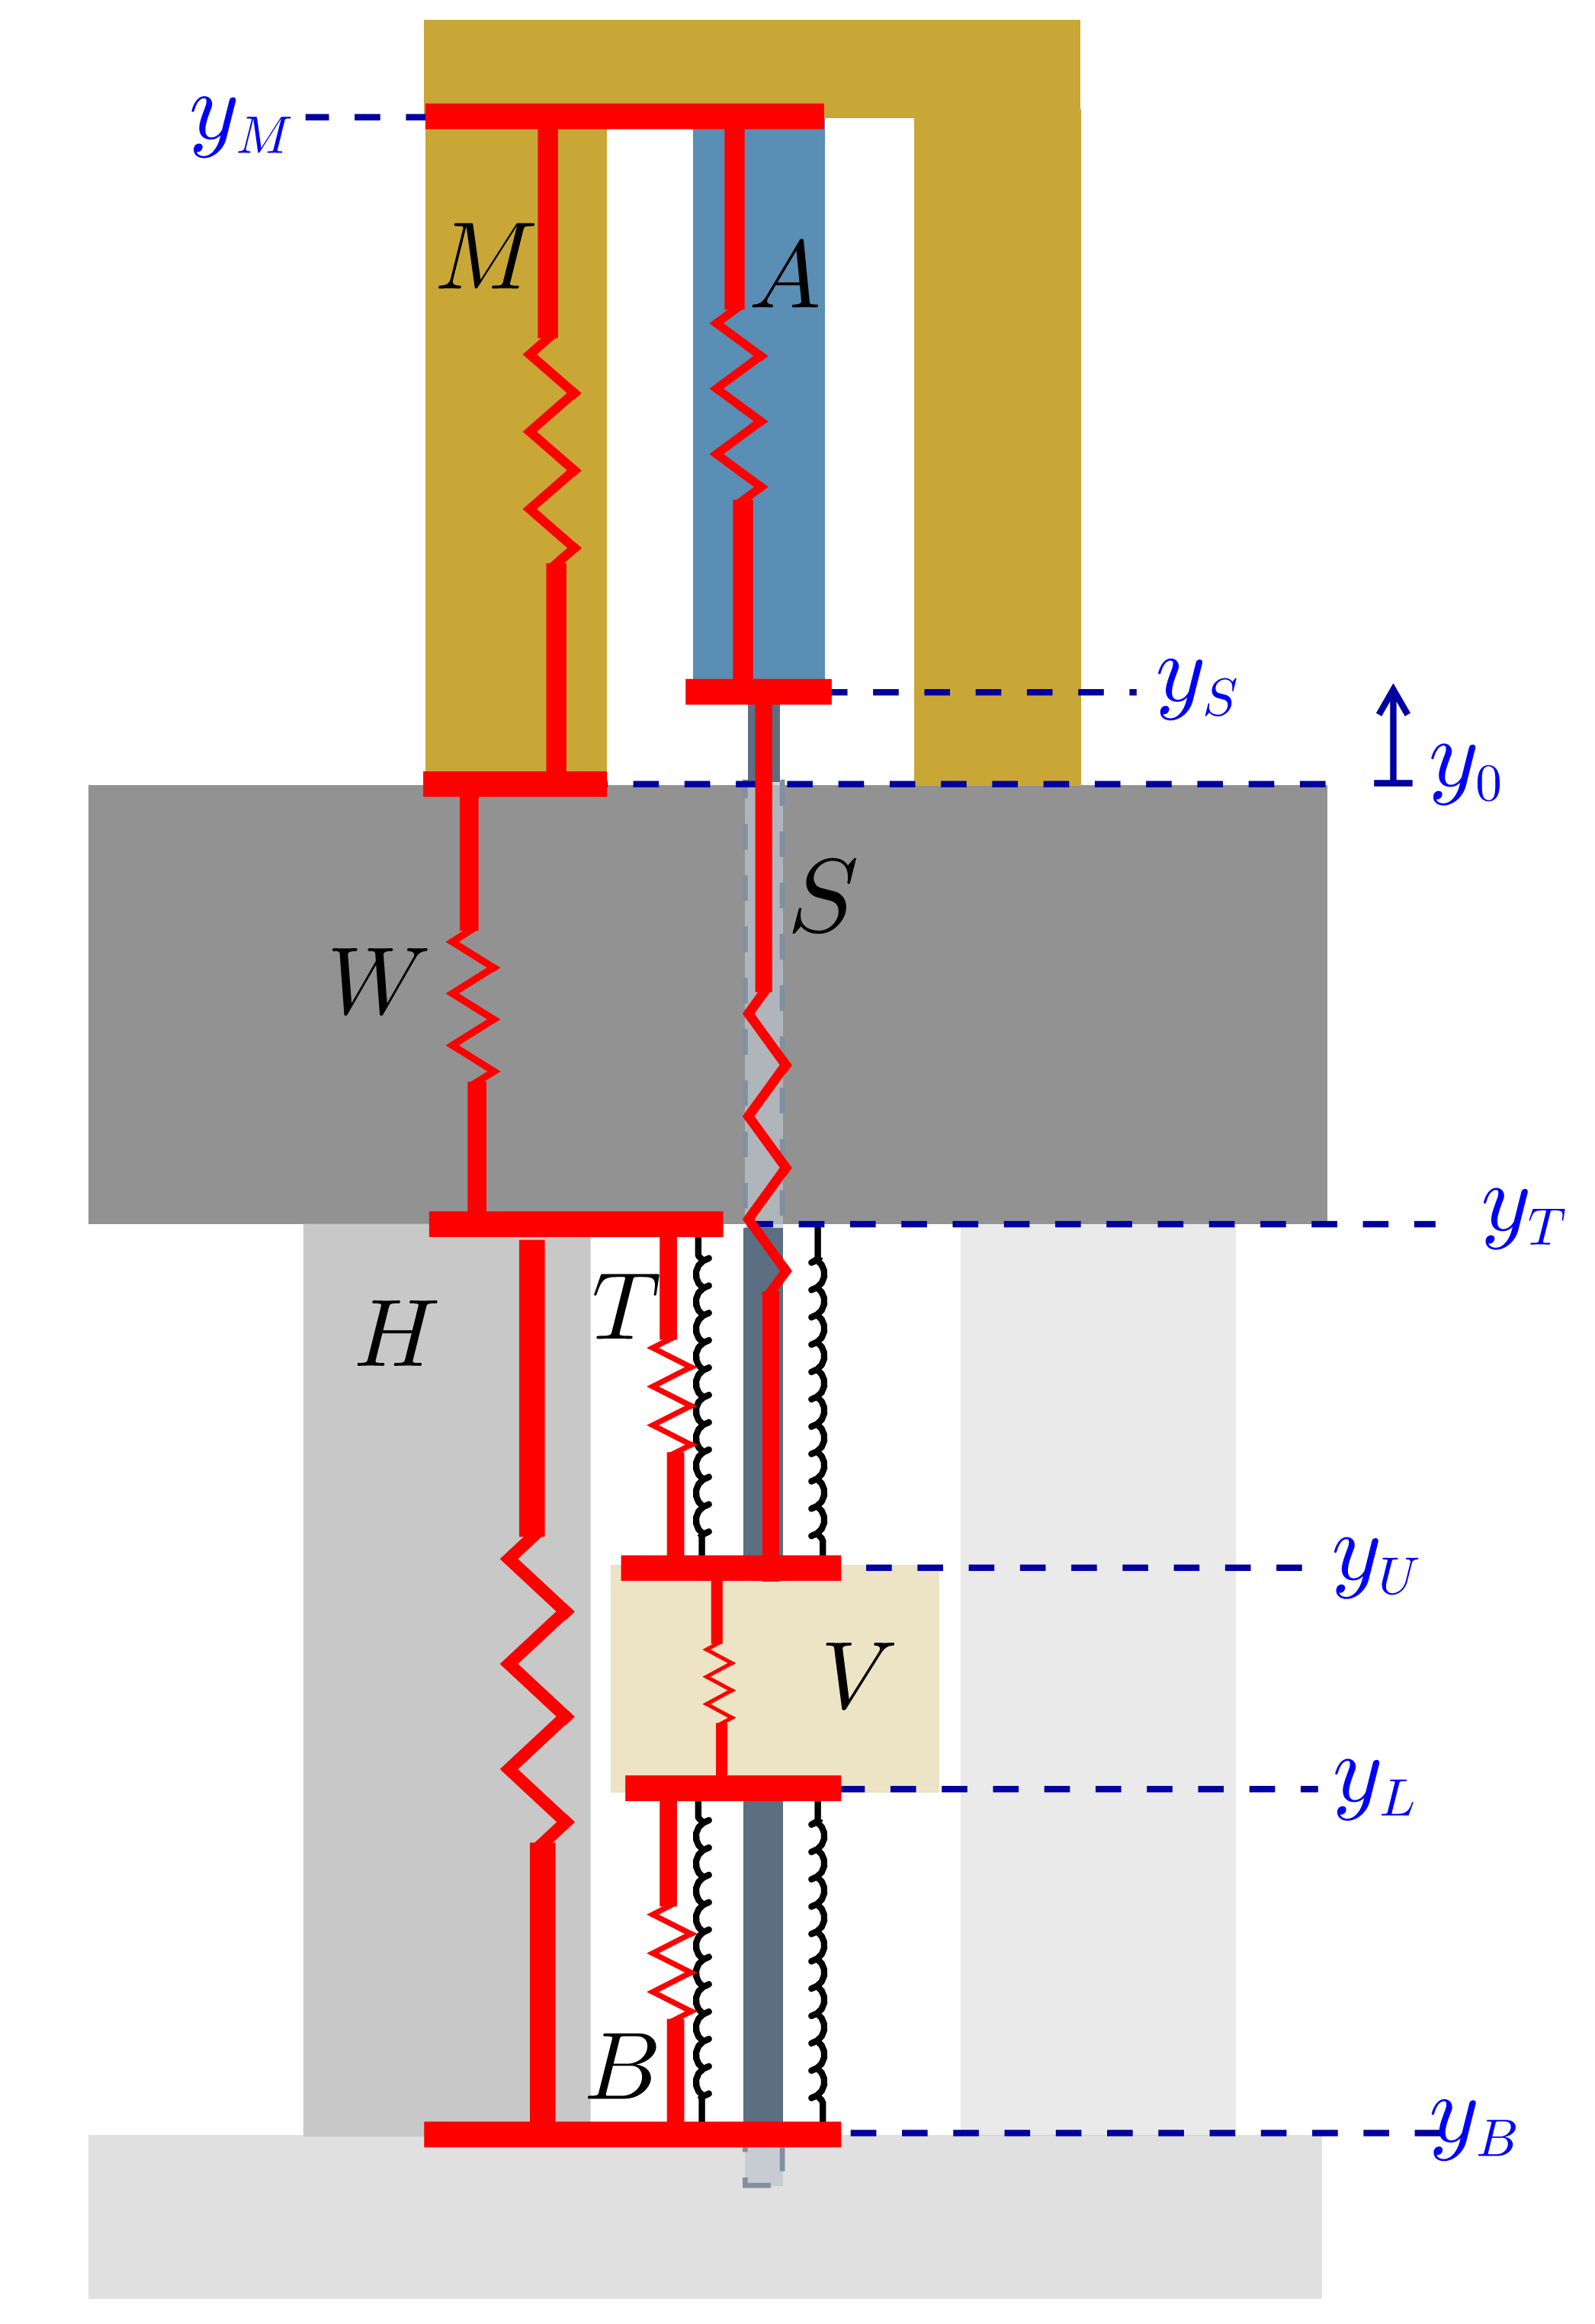
\includegraphics[height=.5\textheight]{springs.png}
					\subcaption{\device\ spring mechanism}
					\label{fig:springs_full}
				\end{minipage}
				\hfill
				\begin{minipage}{.45\textwidth}
					\centering
					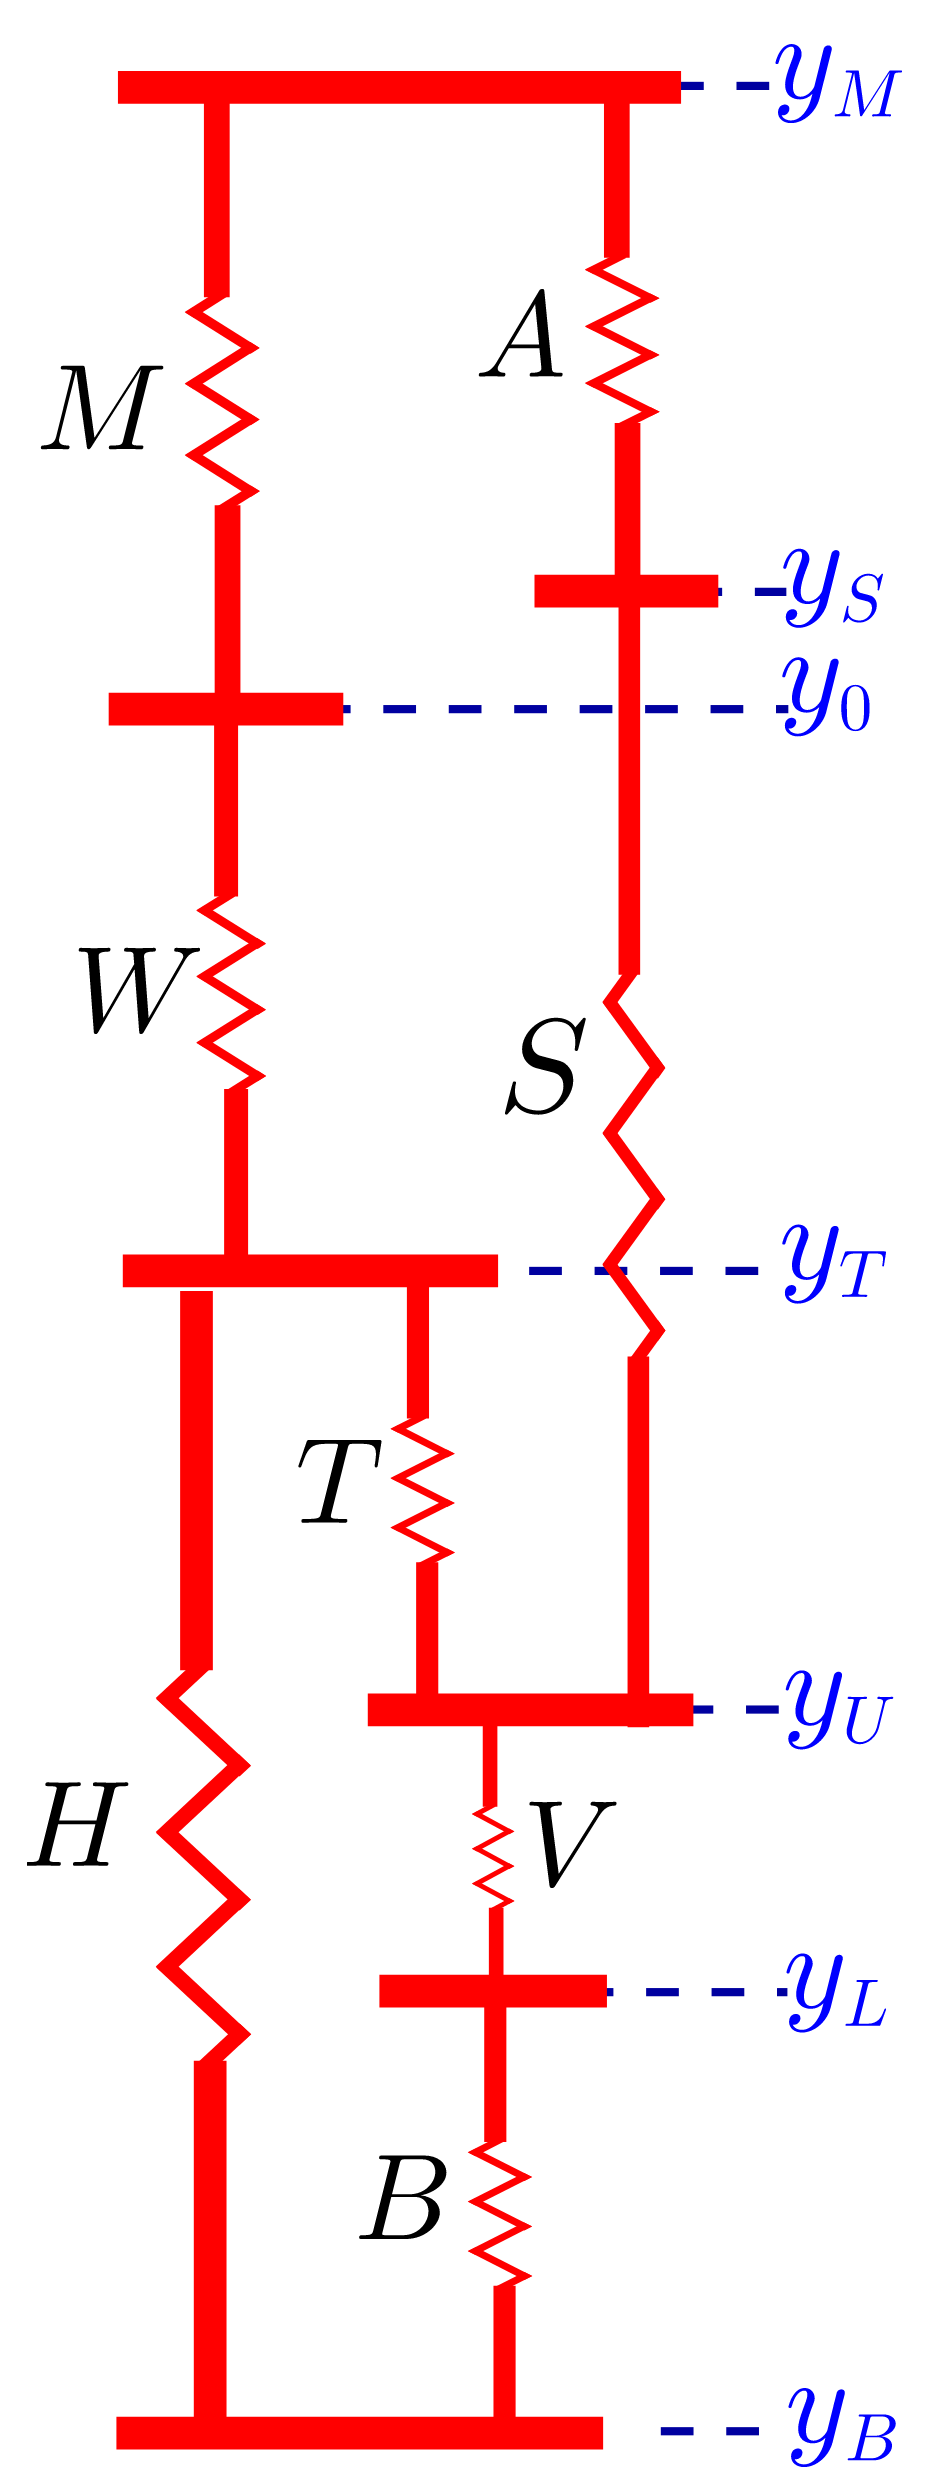
\includegraphics[height=.5\textheight]{springs_simp.png}
					\subcaption{\device\ spring mechanism, simplified}
					\label{fig:springs_simp}
				\end{minipage}
				\caption{Spring deflection}
				\label{fig:springs}
			\end{figure}


			Solution of the final lengths of these springs requires a system of equations, derived using static force analysis.
			We will use Figure~\ref{fig:springs_simp}, which accurately depicts the contact between parts, as our guide.
			The system contains seven nodes, labeled according to their subscripted position $y$, that we will use as the basis for our equations.
			For each nodal force balance, let us assume that the springs act along one degree of freedom (DOF), inducing no rotational moment.
			This is a safe assumption because, although the springs are depicted as spaced apart horizontally, they are concentric in the actual design.

			Equating upper and lower vertical forces at each node produces the following system of equations:

			\newcommand{\circlab}[1]{%
				\tikz[baseline=(char.base)]{
					\node[shape=circle, draw, inner sep=1pt,
						minimum size=1.5em] (char) {$#1$};
				}%
			}

			\newcommand{\ellipselab}[1]{%
				\tikz[baseline=(char.base)]{
					\node[shape=ellipse, draw, inner sep=1pt,
						minimum width=3.2em, minimum height=1.6em] (char) {$#1$};
				}%
			}

			\begin{equation}
				\left\{
				\begin{array}{ll}
					\circlab{y_M} & F_M + F_A = 0 \\[6pt]
					\circlab{y_S} & F_A = F_S \\[6pt]
					\circlab{y_0} & F_M = F_W \\[6pt]
					\circlab{y_T} & F_W = F_H + F_T \\[6pt]
					\circlab{y_U} & F_V = F_T + F_S \\[6pt]
					\circlab{y_L} & F_V = F_B \\[6pt]
					\circlab{y_B} & F_H + F_B = 0 \\
				\end{array}
				\right.
			\end{equation}

			This produces seven equations for eight unknown forces $(F_M, F_A, F_S, F_T, F_B, F_V, F_H, \text{ and } F_W)$.
			One might observe that this system remains indeterminate without one additional equation\footnote{It is well-established in the field of Linear Algebra that a system of linear equations with more equations than unknowns is linearly dependent (one or more equations is redundant) or self-contradictory, while that with more unknowns than equations is incomplete. A determinate system of equations requires exactly as many linearly independent equations as unknowns\cite{ref_Anton}.}.
			In fact, this system is linearly dependent and, when rearranged, contains a pair of redundant equations.

			From Equations $y_M$, $y_S$, and $y_0$:

			\begin{align*}
				F_M &= F_W \\
				F_A &= -F_M = -F_W \\
				F_S &= F_A = -F_W
			\end{align*}

			From Equations $y_L$ and $y_B$:

			\begin{align*}
				F_B &= F_V \\
				F_H &= -F_B = -F_V
			\end{align*}

			Substituting these into Equations $y_T$ and $y_U$:

			\begin{align*}
				F_W &= -F_V + F_T \\
				F_V &= F_T - F_W
			\end{align*}

			These equations are linearly dependent and therefore redundant; one can easily rearrange one to equal the other. Thus, we will strike Equation~$y_U$, leaving us six equations and eight unknowns.

			By Hooke's Law\cite{ref_Young_Freedman}, $F = k \Delta X$, we can substitute their forces for known spring constants, known undeformed lengths (as output by the thermal transfer functions), and unknown final lengths.
			The final two equations are supplied by two parallel length equalities: between $y_M$ and $y_U$ and between $y_T$ and $y_B$.

			\begin{equation}
				\left\{
				\begin{array}{ll}
					\circlab{y_M} & k_M(L_M - \ell_M) + k_A(L_A - \ell_A) = 0 \\[6pt]
					\circlab{y_S} & k_A(L_A - \ell_A) = k_S(L_S - \ell_S) \\[6pt]
					\circlab{y_0} & k_M(L_M - \ell_M) = k_W(L_W - \ell_W) \\[6pt]
					\circlab{y_T} & k_W(L_W - \ell_W) = k_H(L_H - \ell_H) + k_T(L_T - \ell_T) \\[6pt]
					\circlab{y_L} & k_V(L_V - \ell_V) = k_B(L_B - \ell_B) \\[6pt]
					\circlab{y_B} & k_H(L_H - \ell_H) + k_B(L_B - \ell_B) = 0 \\[6pt]
					\ellipselab{y_M \rightarrow y_U} & L_M + L_W + L_T = L_A + L_S \\[6pt]
					\ellipselab{y_T \rightarrow y_B} & L_H = L_T + L_V + L_B
				\end{array}
				\right.
			\end{equation}

			Now we have a system of eight equations with eight unknowns. These can be analytically solved using a matrix calculator by rearranging as follows:

			\begin{equation}
				\left\{
				\begin{array}{l}
					k_M L_M + k_A L_A = k_M \ell_M + k_A \ell_A \\[6pt]
					k_A L_A - k_S L_S = k_A \ell_A - k_S \ell_S \\[6pt]
					k_M L_M - k_W L_W = k_M \ell_M - k_W \ell_W \\[6pt]
					k_W L_W - k_T L_T - k_H L_H = k_W \ell_W - k_T \ell_T - k_H \ell_H \\[6pt]
					k_V L_V - k_B L_B = k_V \ell_V - k_B \ell_B \\[6pt]
					k_B L_B + k_H L_H = k_B \ell_B + k_H \ell_H \\[6pt]
					L_M - L_A - L_S + L_T + L_W = 0 \\[6pt]
					L_T + L_B + L_V - L_H = 0
				\end{array}
				\right.
			\end{equation}

			\begin{equation}
				\begin{bmatrix}
					k_M & k_A  & 0    & 0     & 0     & 0     & 0     & 0     \\
					0   & k_A  & -k_S & 0     & 0     & 0     & 0     & 0     \\
					k_M & 0    & 0    & 0     & 0     & 0     & 0     & -k_W  \\
					0   & 0    & 0    & -k_T  & 0     & 0     & -k_H  & k_W   \\
					0   & 0    & 0    & 0     & -k_B  & k_V   & 0     & 0     \\
					0   & 0    & 0    & 0     & k_B   & 0     & k_H   & 0     \\
					1   & -1   & -1   & 1     & 0     & 0     & 0     & 1    \\
					0   & 0    & 0    & 1     & 1     & 1     & -1    & 0
				\end{bmatrix}
				\begin{bmatrix}
					L_M \\ L_A \\ L_S \\ L_T \\ L_B \\ L_V \\ L_H \\ L_W
				\end{bmatrix}
				=
				\begin{bmatrix}
					k_M \ell_M + k_A \ell_A \\
					k_A \ell_A - k_S \ell_S \\
					k_M \ell_M - k_W \ell_W \\
					k_W \ell_W - k_T \ell_T - k_H \ell_H \\
					k_V \ell_V - k_B \ell_B \\
					k_H \ell_H + k_B \ell_B \\
					0 \\
					0
				\end{bmatrix}
				\label{eq:app_matrix}
			\end{equation}

			Each undeformed length $\ell$ is provided by the thermal transfer functions. With the exception of the two bellows, whose spring constants are given, each spring constant $k$ is calculated by material properties and part geometry\cite[Eq.~4-2]{ref_Hibbeler}:
			
			\begin{equation}
				k = \frac{EA}{\ell}
				\label{eq:k}
			\end{equation}
			
			where $E$ is the elastic modulus, $A$ is the cross-sectional area, and $\ell$ is defined as before.
			Each piece, though nearly rigid, is slightly flexible and can be modeled as a spring under axial load.
			Equation~\eqref{eq:k} provides the equivalent spring constant for each part, calculated below:
			
			\subsubsection{Mount}
			\label{app:sat:TF:force_balance:M}

				$E_M = E_{\text{ALLVAR}} = \specEALLV$\cite{ref_AllvarAlloys}
				
				$A_M = \frac{\pi}{4} (OD^2 - ID^2) = \frac{\pi}{4} [(\SI{25}{\milli\meter})^2 - (\SI{18}{\milli\meter})^2] = \SI{236.4}{\milli\meter\squared}$

			\subsubsection{Actuator}
			\label{app:sat:TF:force_balance:A}

				$E_A = E_{\text{Aluminum}} = \specEAl$\cite[p.~39]{ref_NASA_specs_Al}

				$A_A = \frac{\pi}{4} D^2 = \frac{\pi}{4} (\SI{18}{\milli\meter})^2 = \SI{254.5}{\milli\meter\squared}$

			\subsubsection{Valve Stem}
			\label{app:sat:TF:force_balance:S}

				$E_S = E_{\text{Invar}} = \specEInv $\cite{ref_Carpenter_Inv}

				$A_S = \frac{\pi}{4} D^2 = \frac{\pi}{4} (\SI{3.353}{\milli\meter})^2 = \SI{2.6}{\milli\meter\squared}$
				
			\subsubsection{Bellows}
			\label{app:sat:TF:force_balance:TB}

				$k_T = k_B = \specBellowsK $\cite{ref_miniflex_design}

			\subsubsection{Valve Orifice}    
			\label{app:sat:TF:force_balance:V}
			
			$E_V = E_{\text{Invar}} = \specEInv $
			
			$A_V = LW = (\SI{7}{\milli\meter}) (\SI{7}{\milli\meter}) = \SI{49}{\milli\meter\squared}$
			
			\subsubsection{Housing}    
			\label{app:sat:TF:force_balance:H}

				$E_H = E_{\text{Invar}} = \specEInv $

				$A_H = LW = (\SI{72}{\milli\meter}) (\SI{40}{\milli\meter}) = \SI{2880}{\milli\meter\squared}$

			\subsubsection{Top wall}
			\label{app:sat:TF:force_balance:W}

				$E_W = E_{\text{Invar}} = \specEInv $

				$A_W = A_H = \SI{2880}{\milli\meter\squared}$

			These spring constants are input into Equation~\eqref{eq:app_matrix} to solve for the deformed length of each part.

		\subsection{Position calculations}
		\label{app:sat:TF:pos}

			Finally, we can use these lengths to calculate the values $y_F$ and $y_R$ of the two orifice components shown in Figure~\ref{fig:positional_block_diagram_zoom}.
			Using the scheme depicted in Figure~\ref{fig:positional_block_diagram}, these are as follows:

				\begin{align}
					y_F &= L_M - L_A - L_S - K_V L_V \label{eq:yF}\\
					y_R &= - K_H (2 L_W + L_H) \label{eq:yR}
				\end{align}

			To reach the upper corner of the leading orifice, which is cut into the Valve Orifice part, from the top surface of the housing (our reference location, where $y=0$),
			one must travel up the mount, down the actuator, down the valve stem, and partway down the valve orifice.
			To reach the lower corner of the trailing orifice, which is cut into the Housing Outlet, from the same reference position,
			one must travel straight down the housing wall.
			Because $L_V$ and $L_H$ represent the total height of the valve orifice and housing outlet, a multiplier is required to find the position of each square cut.
			The scaling constant $K_V$ defines the position of the upper vertex of the leading orifice, and $K_H$ the lower vertex of the trailing orifice, determined by its machined dimensions as shown in Figure~\ref{fig:K_pos}.

			\begin{wrapfigure}{l}{0.5\textwidth}
				\centering
				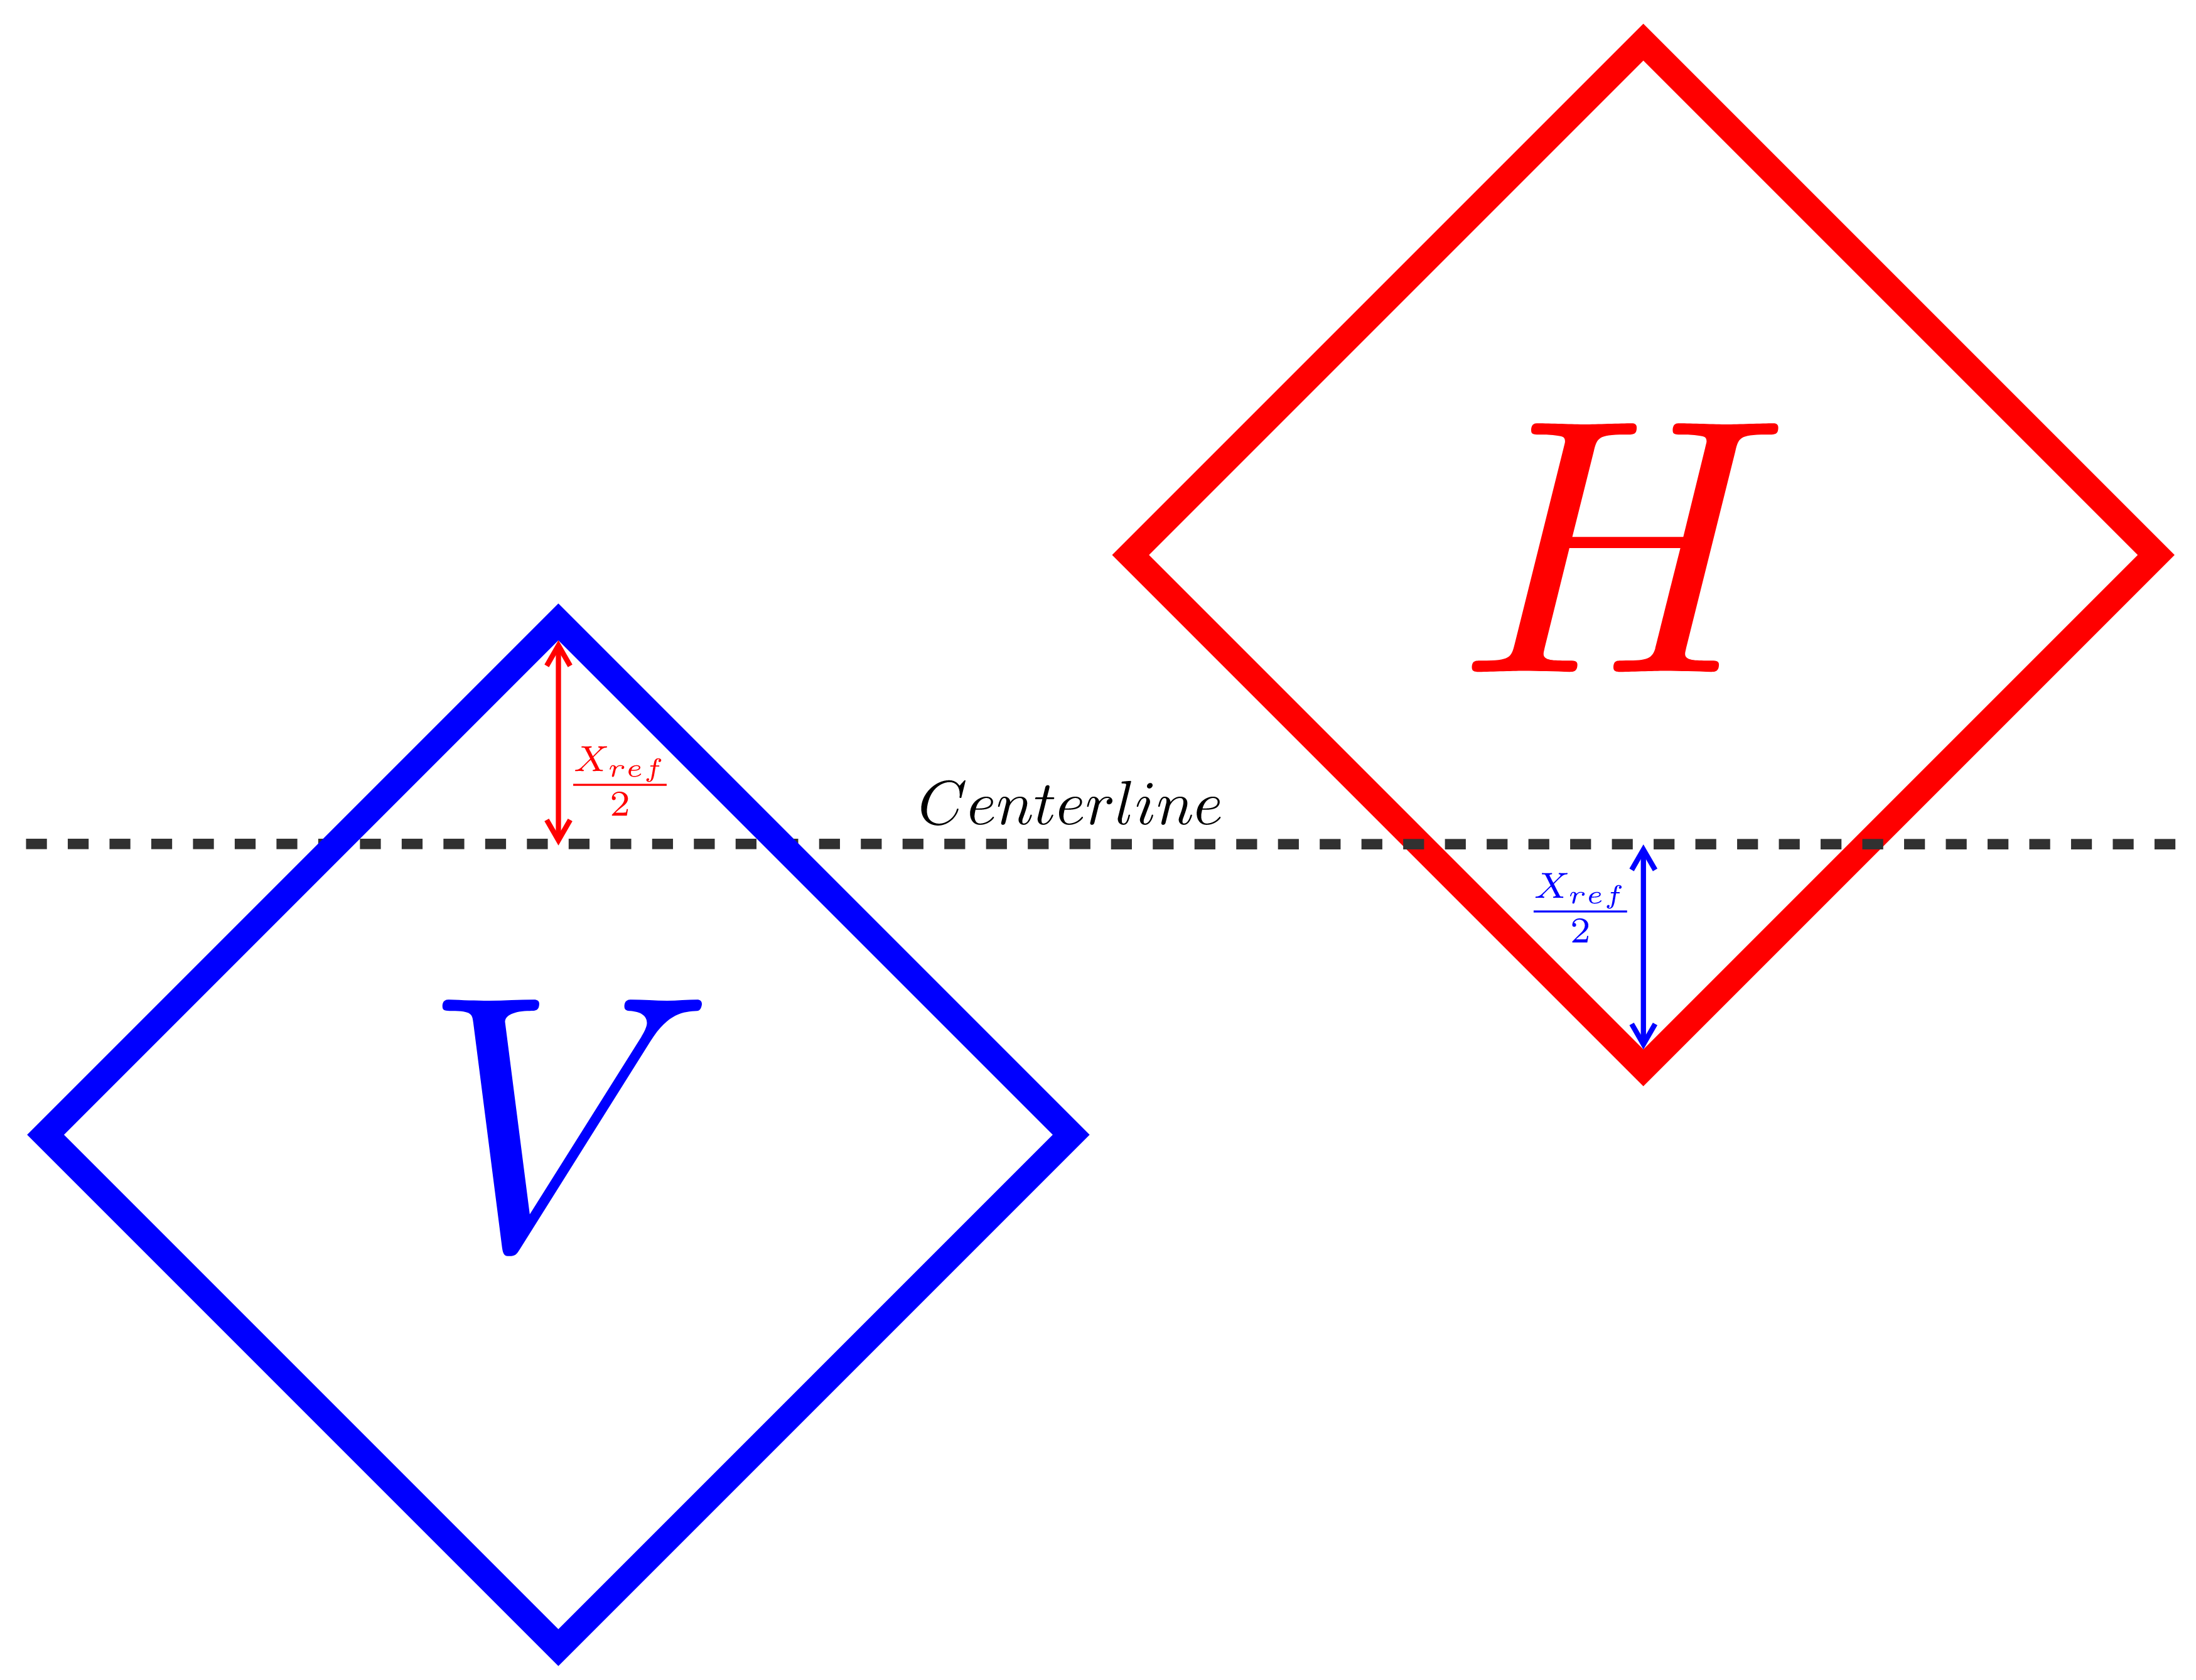
\includegraphics[width=0.48\textwidth]{K_pos.png}
				\caption{Orifice geometry}
				\label{fig:K_pos}
			\end{wrapfigure}

			\newpage
			As manufactured, $K_V \ell_{V_0}$ is defined as the distance from the top surface of the Valve Orifice $(y_T)$, whose machined height equals $\ell_{V_0}$, such that

			\begin{equation}
				K_V \ell_{v_0} = \frac{l_{v_0}}{2} - \left[ \frac{X_{ref}}{2} + d_{V_v} \right]
			\end{equation}

			where $d_{V_v}$ is the vertical position error of the EDM operation (defined as positive in the upwards direction), identical to the horizontal position error.

			Likewise, $K_H (2 \ell_{W_0} + \ell_{H_0})$ is defined as the distance from the top surface of the Housing Outlet $(y_0)$, whose machined height equals $(2 \ell_{W_0} + \ell_{H_0})$, such that

			\begin{equation}
				K_H (2 \ell_{W_0} + \ell_{H_0}) = \frac{(2 \ell_{W_0} + \ell_{H_0})}{2} + \left[ \frac{X_{ref}}{2} - d_{V_v} \right]
			\end{equation}

			therefore

			\begin{align}
				K_V &= \frac{1}{2} - \frac{\frac{X_{ref}}{2} + d \ell_{V_v}}{\ell_{V_0}} \\[6pt]
				K_H &= \frac{1}{2} + \frac{\frac{X_{ref}}{2} - d \ell_{H_v}}{2 \ell_{W_0} + \ell_{H_0}}
			\end{align}

			Note that the machined-length values are exact values as the position of the EDM cut is independent of any dimensional error in the valve orifice or housing outlet.

			Using these constants in Equations~\eqref{eq:yF} and \eqref{eq:yR}, we find the height of the orifice $X$ by taking the difference between the position of the upper and lower corners of the orifice:

				\begin{equation}
					X = y_F - y_R
				\end{equation}

		\newpage

    \subsection{Orifice Geometry}
    \label{app:sat:TF:orif}

			\begin{wrapfigure}{l}{0.35\textwidth}
					\centering
					\includegraphics[width=0.15\textwidth]{G_O.png}
					\caption{Orifice transfer function}
					\label{fig:G_O}
			\end{wrapfigure}

			Finally, with the height of the orifice, we can calculate its effective diameter.
			This is the most critical part of the System Transfer Function because the square orifice bears the most potential for machining errors.
			Such errors will be kept symbolic for now.

			The orifice transfer function $\hat{G}_O$ is best divided into two sub-transfer functions, as in Figure~\ref{fig:G_O}:
			one to convert the orifice into the orifice area $A$, and one to convert area into effective diameter $D_{eff}$.

			\subsubsection{$\hat{G}_A$: Height to Area}
			\label{app:sat:TF:orif:G_A}

				Under ideal machining conditions, the orifice area is calculated as follows:

				\begin{equation}
					A = s^2 = \left( \frac{X}{\sqrt{2}} \right)^2 = \frac{X^2}{2}
				\end{equation}

				Each fillet radius $R_f$ subtracts the following area from the orifice, depicted in Figure~\ref{fig:Rf}:

				\begin{equation}
					dA = (\textit{Orange area}) = (\textit{Square area}) - (\textit{Gray quarter circle}) = R_f^2 - \frac{1}{4} \pi R_f^2 = \frac{1}{4} (4 - \pi) R_f^2
				\end{equation}

				\begin{figure}[H]
					\centering
					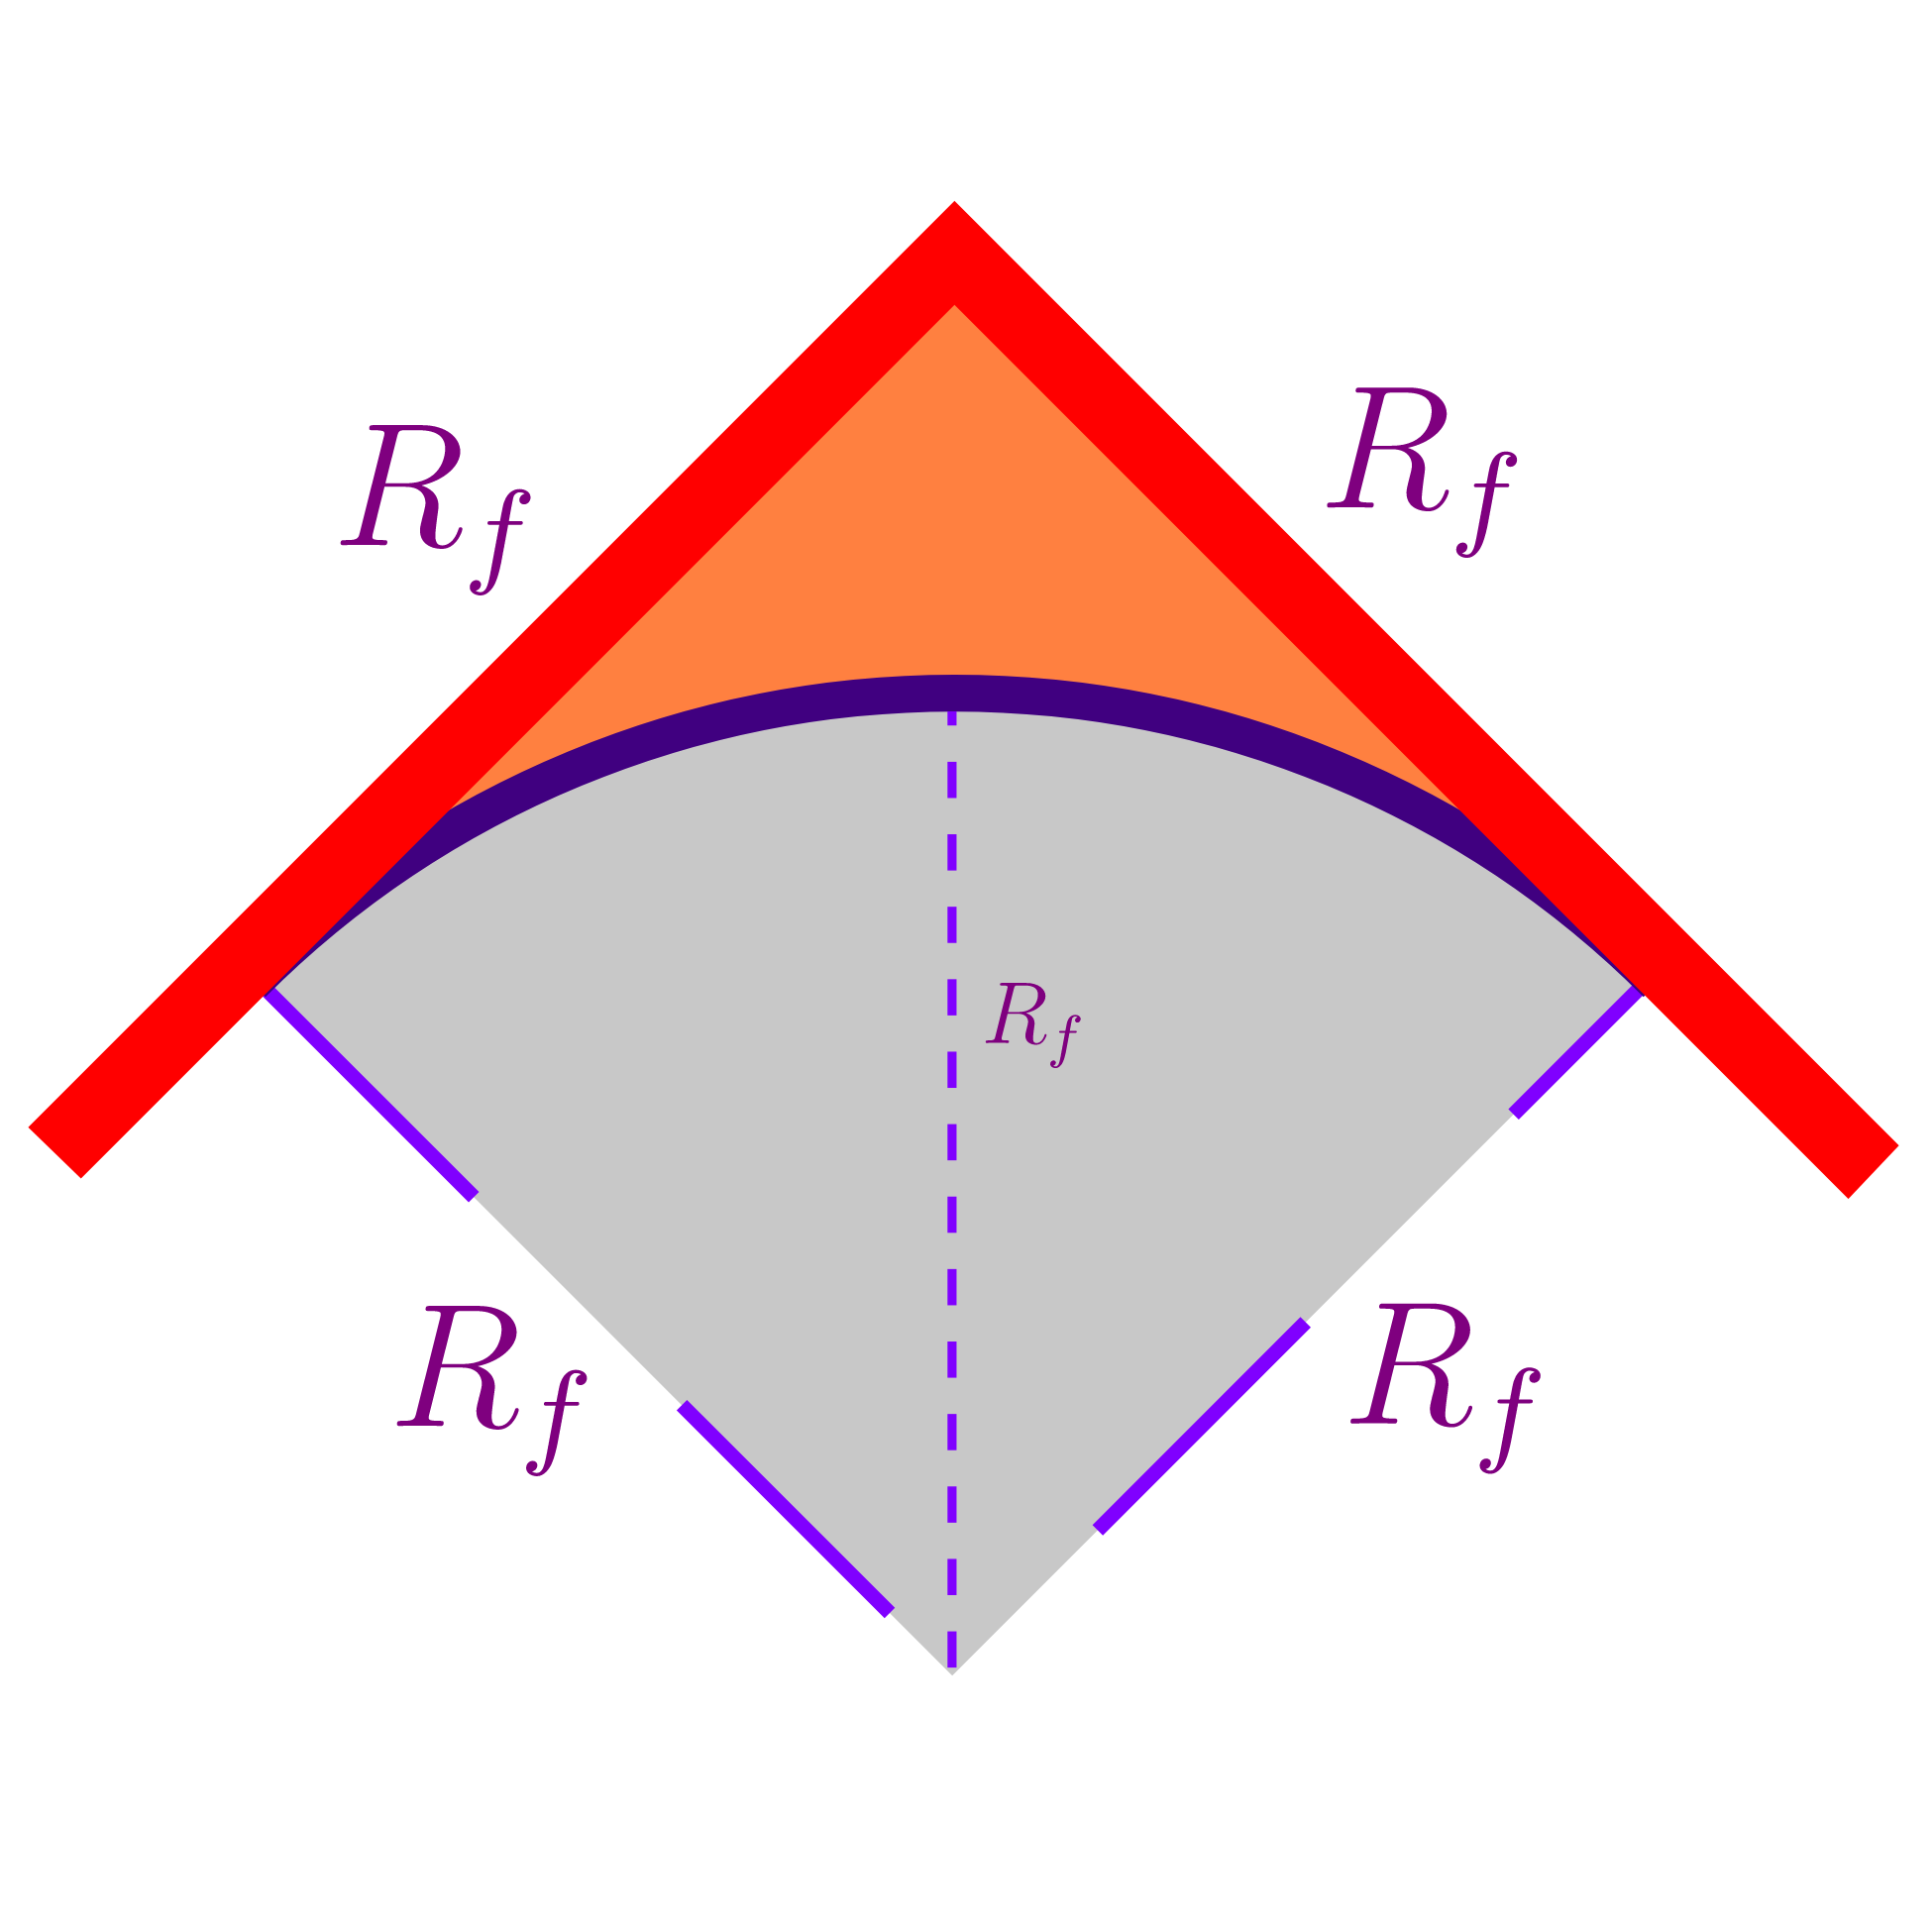
\includegraphics[width=.3\textwidth]{Rf.png}
					\caption{Fillet radius dimensions}
					\label{fig:Rf}
				\end{figure}

				Horizontal shift $d \ell_h$ changes the area as shown in Figure~\ref{fig:dl_h}, adding the green area and subtracting the orange.
				Ignoring the fillet radii, this results in the new area

				\begin{equation}
					A = (s + \frac{d \ell}{2}) (s - \frac{d \ell}{2}) = s^2 - \frac{d \ell^2}{2}
				\end{equation}

				\begin{figure}[H]
					\centering
					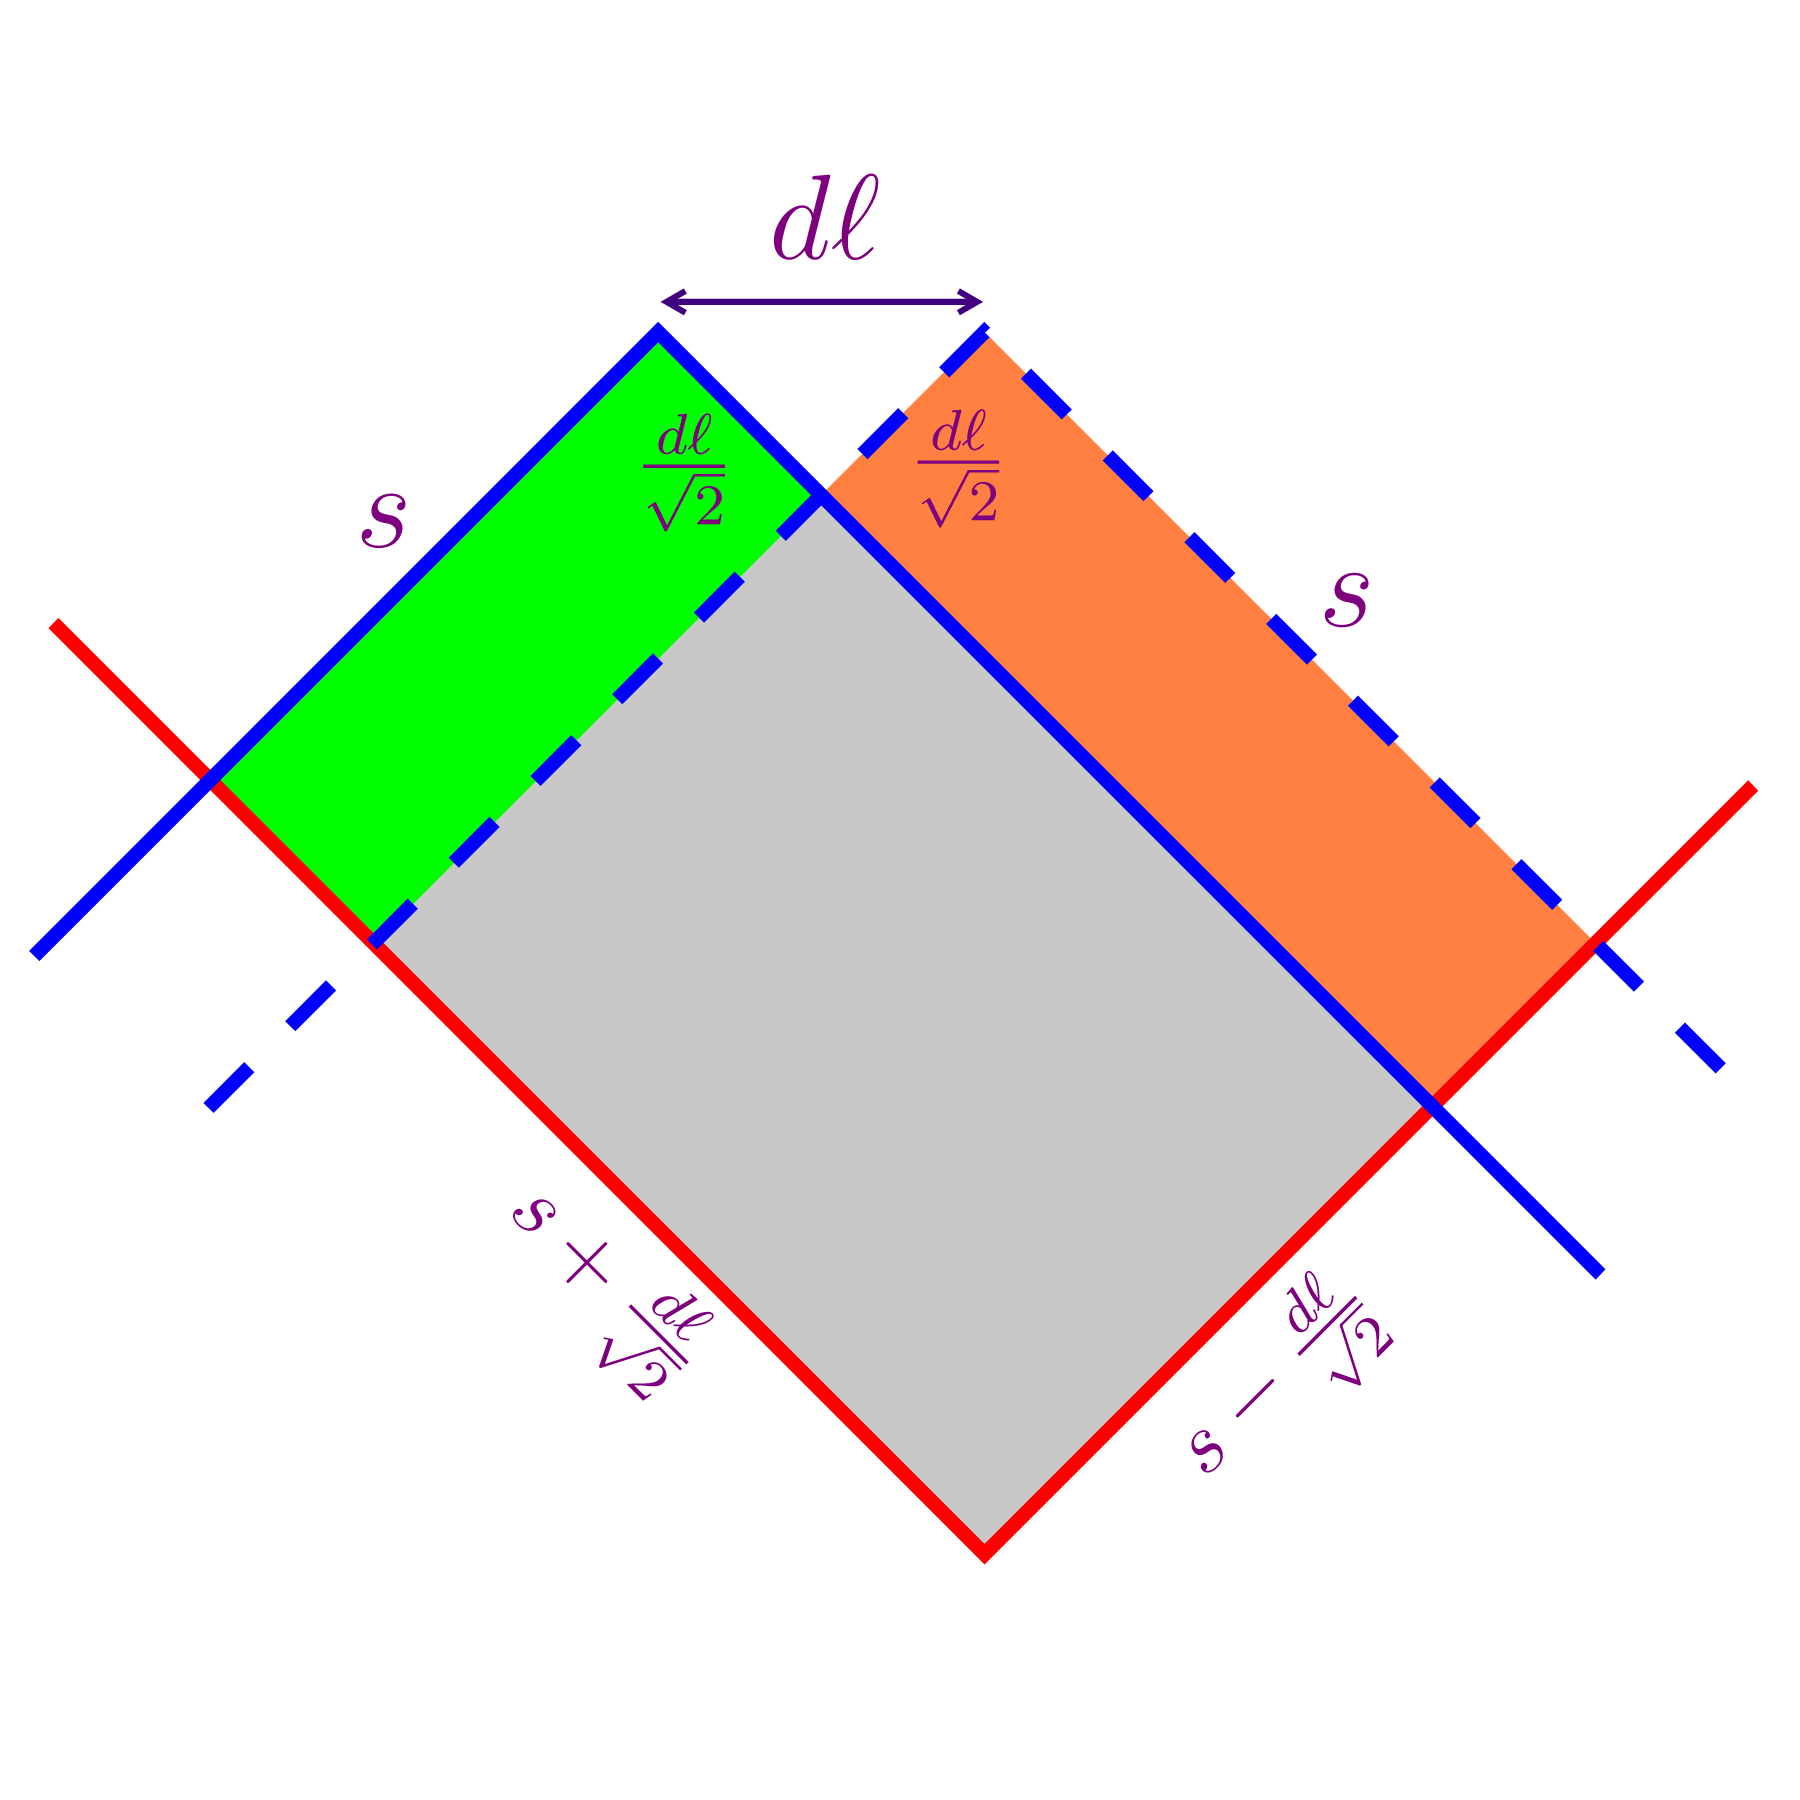
\includegraphics[width=.3\textwidth]{dl_h.png}
					\caption{Horizontal offset dimensions}
					\label{fig:dl_h}
				\end{figure}

				yielding the final orifice area:

				\begin{equation}
					A = s^2 - \frac{1}{2} \left[ (4 - \pi) R_f^2 - d \ell^2 \right]
					\label{eq:GA}
				\end{equation}

				The minimum achievable fillet radius and positional tolerance are \SI{76.2}{\micro\meter} and \SI{12.7}{\micro\meter},
				as quoted by Milco Wire EDM, Inc (Appendix~\ref{app:BOM}). These are input into the Transfer Function when numerically evaluated.

			\subsubsection{$\hat{G}_D$: Area to Effective Diameter}
			\label{app:sat:TF:orif:G_D}
				
				The area-diameter conversion is a simple geometric calculation, where $D_{eff}$ is the diameter of a circle with equivalent area. Thus,

				\begin{equation}
					D_{eff} = \sqrt{\frac{4}{\pi} A}
				\end{equation}

			therefore

				\begin{equation}
					\hat{G}_O = \sqrt{\frac{4}{\pi} \left( s^2 - \frac{1}{2} \left[ (4 - \pi) R_f^2 - d \ell^2 \right] \right)}
				\end{equation}

		\subsection{Transfer Function Results}
		\label{app:sat:TF:results}

			The System Transfer Function can be computed using a simple script, which calculates each sub-transfer function as derived above and the force balance using a matrix solver.
			The script was tested with ideal conditions; its output matched the Required Relationship exactly at every temperature.
			Error was then input into the function. Some errors are deterministic or demonstrate an objective worst-case values: variations in aluminum's CTE, spring force deflections, the fillet radius, and effective temperatures.
			The rest --- namely, all vertical dimensional errors ($d \ell_M$, $d \ell_A$, $d \ell_S$, $d \ell_V$, $d \ell_H$, and $d \ell_W$)
			and the vertical and horizontal positions of each orifice ($d \ell_{V_v}$, $d \ell_{H_v}$, $d \ell_{V_h}$, and $d \ell_{H_h}$) ---
			are stochastic. In other words, the value of each will vary each time the part is produced due to slight imprecisions in the machining process
			and cannot be exactly predicted.

			Figure~\ref{fig:TF_res} demonstrates the output of the System Transfer Function given two worst-case combinations of the stochastic error values:
			$d \ell_M$, $d \ell_A$, $d \ell_S$, $d \ell_V$, $d \ell_H$, $d \ell_W$, $d \ell_{V_v}$, $d \ell_{H_v}$, $d \ell_{V_h}$, and $d \ell_{H_h}$.
			These serve as the expected boundaries for any system output across prototypes.
			If many identical devices are manufactured, most will achieve their required tolerance without calibration, but some will reach these boundaries and fall outside of tolerance.
			The lower boundary represents the combination of errors where the effective diameter is the smallest --- the valve stem is positioned lower than it should be.
			The upper boundary represents the opposite.

			Each stochastic machining error follows a normal distribution, where its tolerable range holds approximately six standard deviations $(6 \sigma)$ for a typical Computer-Numerical Control (CNC) machine\cite{ref_AIAG2005}.
			Producing a normalized distribution expectation plot via Monte Carlo analysis\cite{ref_figliola},
			which evaluates $10^6$ samples, each with a different random combination of stochastic inputs and finds the resulting error distribution,
			the function demonstrated that 90.6\% of devices are expected to achieve the Required Relationship without needing calibration.
			It output the normalized distribution in Figure~\ref{fig:error_dist}, with a mean of -45.2\% and a standard deviation of 41.5\%, measured as a percentage of the tolerance window at $T_{ref}$ (where the tolerance is narrowest).
			On average, a freshly-assembled device will produce an orifice that is smaller than nominal by half its tolerance window.
			Those that fall outside of tolerance do not exceed their boundary by more than \SI{44.6}{\micro\meter}.
			These can be remedied using the calibration stack, whose range is sufficient to correct the maximum errors anticipated by the Transfer Function.

			\begin{figure}[h]
				\centering
				\begin{tikzpicture}
				\begin{axis}[
								width       = 14cm,
								height      = 8cm,
								xlabel      = {Ambient Temperature ($^\circ$C)},
								ylabel      = {Actual Effective Diameter ($\upmu$m)},
								xmin = -70, xmax = 90,
								ymin = 80,  ymax = 450,
								grid        = major,
								major grid style = {line width=0.4pt, draw=gray!50},
								minor tick num   = 0,
								tick align  = inside,
								legend pos  = north east,
								legend style     = {font=\small},
								tick label style = {font=\small},
								label style      = {font=\small},
				]

				%% ── Gold TF paths (named, no fill yet) ────────────────────────────────
				\addplot [
								name path   = TF_high,
								color       = ucdgold,
								line width  = 1.6pt,
								dash dot,
								forget plot,
				] table [
								x expr      = \thisrow{T_amb_C},
								y expr      = \thisrow{D_TF_high} * 1e6,
								col sep     = comma,
				] {csv/TF.csv};

				\addplot [
								name path   = TF_low,
								color       = ucdgold,
								line width  = 1.6pt,
								dashed,
								forget plot,
				] table [
								x expr      = \thisrow{T_amb_C},
								y expr      = \thisrow{D_TF_low} * 1e6,
								col sep     = comma,
				] {csv/TF.csv};

				%% ── Gold fill ─────────────────────────────────────────────────────────
				\addplot [
								fill        = ucdgold!20,
								draw        = none,
								forget plot,
				] fill between [of = TF_high and TF_low];

				%% ── Blue tolerance paths (named, no fill yet) ─────────────────────────
				\addplot [
								name path   = lower,
								color       = ucdblue,
								line width  = 0.8pt,
								dotted,
								forget plot,
				] table [
								x expr      = \thisrow{T_amb_C},
								y expr      = \thisrow{D_eff_lower} * 1e6,
								col sep     = comma,
				] {csv/TF.csv};

				\addplot [
								name path   = upper,
								color       = ucdblue,
								line width  = 0.8pt,
								dotted,
								forget plot,
				] table [
								x expr      = \thisrow{T_amb_C},
								y expr      = \thisrow{D_eff_upper} * 1e6,
								col sep     = comma,
				] {csv/TF.csv};

				%% ── Blue fill (on top of gold) ────────────────────────────────────────
				\addplot [
								fill        = sandiablue!20,
								draw        = none,
								forget plot,
				] fill between [of = lower and upper];

				%% ── Nominal required line ─────────────────────────────────────────────
				\addplot [
								color       = ucdblue,
								line width  = 1.6pt,
								forget plot,
				] table [
								x expr      = \thisrow{T_amb_C},
								y expr      = \thisrow{D_eff_nominal} * 1e6,
								col sep     = comma,
				] {csv/TF.csv};

				%% ── Monte Carlo mean output (all stochastic errors = 0, R_f applied) ──
				\addplot [
								color       = ucdgold,
								line width  = 1.6pt,
								solid,
								forget plot,
				] table [
								x expr      = \thisrow{T_amb_C},
								y expr      = \thisrow{D_TF_mean} * 1e6,
								col sep     = comma,
				] {csv/TF.csv};

				%% ── Legend entries ────────────────────────────────────────────────────
				\addplot [color=ucdblue, line width=1.6pt]
								coordinates {(-200,0)};
				\addlegendentry{Nominal output}

				\addplot [color=ucdblue, line width=0.8pt, dotted]
								coordinates {(-200,0)};
				\addlegendentry{Tolerance band}

				\addplot [color=ucdgold, line width=1.6pt, solid]
								coordinates {(-200,0)};
				\addlegendentry{Mean output}

				\addplot [color=ucdgold, line width=1.6pt, dash dot]
								coordinates {(-200,0)};
				\addlegendentry{Stochastic boundaries}

				\end{axis}
				\end{tikzpicture}%
				\caption{Transfer Function output range}
				\label{fig:TF_res}
			\end{figure}

			\vspace{1em}
			\begin{figure}[h]
					\centering
					\begin{tikzpicture}
					\begin{axis}[
							width       = 14cm,
							height      = 8cm,
							xlabel      = {Error (\% tolerance window at $T_{ref}$)},
							ylabel      = {Probability Density},
							xmin = -250, xmax = 150,
							ymin = 0,    ymax = 0.011,
							grid        = major,
							major grid style = {line width=0.4pt, draw=gray!50},
							minor tick num   = 0,
							tick align  = inside,
							tick label style = {font=\small},
							label style      = {font=\small},
							yticklabel style = {
									/pgf/number format/precision=4,
							},
					]

					%% ── ±100% tolerance window background ───────────────────────────────────
					\addplot [
							name path = tol_lo,
							draw      = none,
							domain    = -100:100,
							samples   = 2,
							forget plot,
					] {0};
					\addplot [
							name path = tol_hi,
							draw      = none,
							domain    = -100:100,
							samples   = 2,
							forget plot,
					] {0.011};
					\addplot [
							fill       = ucdgold!18,
							draw       = none,
							forget plot,
					] fill between [of = tol_lo and tol_hi];

					%% ── ±2σ shaded band ──────────────────────────────────────────────────────
					% ±2σ bounds: μ ± 2σ = -45.1746 ± 83.0826 → [-128.257, 37.908]
					\addplot [
							name path = twosig_lo,
							draw      = none,
							domain    = -128.257:37.908,
							samples   = 2,
							forget plot,
					] {0};
					\addplot [
							name path = twosig_hi,
							draw      = none,
							domain    = -128.257:37.908,
							samples   = 200,
							forget plot,
					] {normalpdf(x, -45.1746, 41.5413)};
					\addplot [
							fill       = sandiablue!15,
							draw       = none,
							forget plot,
					] fill between [of = twosig_lo and twosig_hi];

					%% ── ±1σ shaded band ──────────────────────────────────────────────────────
					% ±1σ bounds: μ ± σ = -45.1746 ± 41.5413 → [-86.716, -3.633]
					\addplot [
							name path = onesig_lo,
							draw      = none,
							domain    = -86.716:-3.633,
							samples   = 2,
							forget plot,
					] {0};
					\addplot [
							name path = onesig_hi,
							draw      = none,
							domain    = -86.716:-3.633,
							samples   = 200,
							forget plot,
					] {normalpdf(x, -45.1746, 41.5413)};
					\addplot [
							fill       = sandiablue!30,
							draw       = none,
							forget plot,
					] fill between [of = onesig_lo and onesig_hi];

					%% ── Normal PDF ───────────────────────────────────────────────────────────
					\addplot [
							color      = ucdgold,
							line width = 1.6pt,
							solid,
							domain     = -250:150,
							samples    = 300,
							forget plot,
					] {normalpdf(x, -45.1746, 41.5413)};

					%% ── σ callout labels ─────────────────────────────────────────────────────
					\node[font=\small, align=center]
							at (axis cs: -45.1746, 0.005)
							{$\pm1\sigma$};

					\node[font=\small, align=center]
							at (axis cs: -105, 0.001)
							{$\pm2\sigma$};
					\node[font=\small, align=center]
							at (axis cs: 15, 0.001)
							{$\pm2\sigma$};

					%% --- Tolerance band --------------------------------
					\node[font=\small, align=center]
							at (axis cs: 0, 0.0102)
							{\textit{Tolerance window}};

					%% --- Percentage compliance ----------------------------
					\node[font=\small, align=center]
							at (axis cs: -45.1746, 0.003)
							{\textit{90.6\%}};
					\node[font=\small, align=center]
							at (axis cs: -45.1746, 0.0023)
							{\textit{compliance}};

					\end{axis}
					\end{tikzpicture}
					\caption{Stochastic error distribution}
					\label{fig:error_dist}
			\end{figure}

			As detailed in Appendix~\ref{app:mfg}, calibration will be performed at approximately $T_{ref}$.
			The maximum expected error at this temperature, as calculated by the Transfer Function, is \SI{30.7}{\micro\meter} and \SI{44.6}{\micro\meter} above and below the nominal reference diameter of

			\begin{equation}
				\Dref
			\end{equation}

			At a minimum, the calibration assembly must be able to correct the error at the extrema by the largest deviation value to the specified tolerance. Thus,

			\begin{equation}
				\Delta D_{cal} \geq 45 \pm 12.7\si{\micro\meter}
			\end{equation}

			Assuming exactly these calibration capabilities, the Transfer Function evaluated the new system output boundaries.
			As shown in Figure~\ref{fig:TF_cal}, these now fall just within the required tolerance window despite several persistent sources of error.
			As discussed in Section~\ref{app:calcs:cal:sat}, the user will likely be able to exceed this tolerance, resulting in a system output well within the required tolerance across the whole temperature range.

			Although calibration corrects the static offset introduced by the vertical dimension errors that affect the orifice height, several errors persist after calibration that change the temperature-diameter slope or introduce nonlinearity.

			\begin{enumerate}
				\item Deviation from the assumed \SI{50}{\micro\meter} compression of the belleville washer will effectively change the mount's machined length, allowing the mount to expand or contract slightly more or less than designed.
					This cannot be avoided. The function accounted for this change when producing Figure~\ref{fig:TF_cal}; it accounts for the erroneous initial slopes.
					At colder temperatures, where the diameter is larger and nonlinear errors (discussed below) take less effect, one can see that the upper bound slopes away from the nominal output.
					This represents devices whose diameter has been reduced by calibration, decompressing the belleville washer and shrinking the mount's expandable length.
					The effective diameter decreases slightly less than required because the mount provides slightly less actuation.
					One would expect the lower bound to exhibit the opposite effect, its mount having been increased by washer compression.
					However, it follows a similar, though subtler, shallow initial slope before being pulled downwards by the orifice machining errors.
					The source of this discrepancy is not certain.
				\item The fillet radius and horizontal position error cannot be corrected. These subtract a constant area, disproportionately reducing the effective diameter towards the hotter temperatures, where the diameter is smallest.
					One can see its effect on the right side of Figure~\ref{fig:TF_cal}, where the expected output diameter drops off at an increasing rate.
					Those devices that produce too large a diameter will conveniently approach the setpoint.
					Those that produce too small a diameter will show greater error on that end, but are expected to remain within tolerance as the window widens toward the extrema.
					The effect is negligible, but if future iterations require compensation for higher temperatures with a smaller diameter, better methods will need to be developed to correct or reduce this error mode.
			\end{enumerate}

			\begin{figure}[H]
					\centering
					\begin{tikzpicture}
					\begin{axis}[
							width       = 14cm,
							height      = 8cm,
							xlabel      = {Ambient Temperature ($^\circ$C)},
							ylabel      = {Actual Effective Diameter ($\upmu$m)},
							xmin = -70, xmax = 90,
							ymin = 80,  ymax = 450,
							grid        = major,
							major grid style = {line width=0.4pt, draw=gray!50},
							minor tick num   = 0,
							tick align  = inside,
							legend pos  = north east,
							legend style     = {font=\small},
							tick label style = {font=\small},
							label style      = {font=\small},
					]

					%% ── Gold TF calibrated paths (named, no fill yet) ─────────────────────
					\addplot [
							name path   = TF_high_cal,
							color       = ucdgold,
							line width  = 1.6pt,
							dash dot,
							forget plot,
					] table [
							x expr      = \thisrow{T_amb_C},
							y expr      = \thisrow{D_TF_high_cal} * 1e6,
							col sep     = comma,
					] {csv/TF_cal.csv};

					\addplot [
							name path   = TF_low_cal,
							color       = ucdgold,
							line width  = 1.6pt,
							dashed,
							forget plot,
					] table [
							x expr      = \thisrow{T_amb_C},
							y expr      = \thisrow{D_TF_low_cal} * 1e6,
							col sep     = comma,
					] {csv/TF_cal.csv};

					%% ── Gold fill ─────────────────────────────────────────────────────────
					\addplot [
							fill        = ucdgold!20,
							draw        = none,
							forget plot,
					] fill between [of = TF_high_cal and TF_low_cal];

					%% ── Blue tolerance paths (named, no fill yet) ─────────────────────────
					\addplot [
							name path   = lower_cal,
							color       = ucdblue,
							line width  = 0pt,
							dotted,
							forget plot,
					] table [
							x expr      = \thisrow{T_amb_C},
							y expr      = \thisrow{D_eff_lower} * 1e6,
							col sep     = comma,
					] {csv/TF_cal.csv};

					\addplot [
							name path   = upper_cal,
							color       = ucdblue,
							line width  = 0pt,
							dotted,
							forget plot,
					] table [
							x expr      = \thisrow{T_amb_C},
							y expr      = \thisrow{D_eff_upper} * 1e6,
							col sep     = comma,
					] {csv/TF_cal.csv};

					%% ── Blue fill ─────────────────────────────────────────────────────────
					\addplot [
							fill        = sandiablue!20,
							draw        = none,
							forget plot,
					] fill between [of = lower_cal and upper_cal];

					%% ── Nominal required line ─────────────────────────────────────────────
					\addplot [
							color       = ucdblue,
							line width  = 1.6pt,
							forget plot,
					] table [
							x expr      = \thisrow{T_amb_C},
							y expr      = \thisrow{D_eff_nominal} * 1e6,
							col sep     = comma,
					] {csv/TF_cal.csv};

					%% ── Legend entries ────────────────────────────────────────────────────
					\addplot [color=ucdblue, line width=1.6pt]
							coordinates {(-200,0)};
					\addlegendentry{Nominal output}

					\addplot [color=ucdblue, line width=0.8pt, dotted]
							coordinates {(-200,0)};
					\addlegendentry{Tolerance band}

					\addplot [color=ucdgold, line width=1.6pt, dash dot]
							coordinates {(-200,0)};
					\addlegendentry{Calibrated boundaries}

					\end{axis}
					\end{tikzpicture}%
					\caption{Transfer Function output range after calibration}
					\label{fig:TF_cal}
			\end{figure}

			The Transfer Function accomplishes two objectives. First, it demonstrates the viability of the \device\ despite its strict output requirement. 90\% of manufactured devices are expected to meet their
			tolerance window; those that do not can be readily calibrated. As is addressed in Section~\ref{subsec:DFMEA::tol} and Chapter~\ref{chap:concl}, this computation does not account for all sources of error and therefore presents an optimistic
			expectation value for the system performance. However, it verifies that the major anticipated errors have been mitigated to a tolerable amount by the design strategies illustrated in Section~\ref{sec:design:just}.
			Second, it provides a ready tool for further iteration. Appendix~\ref{app:iter:customize} provides guidance to use this Transfer Function and its associated software to more quickly evaluate the impact of design changes and improvements.


\chapter{Project Management}
\label{app:PM}


	\begin{figure}[H]
		\centering
		\begin{minipage}[t]{0.45\textwidth}
			\centering
			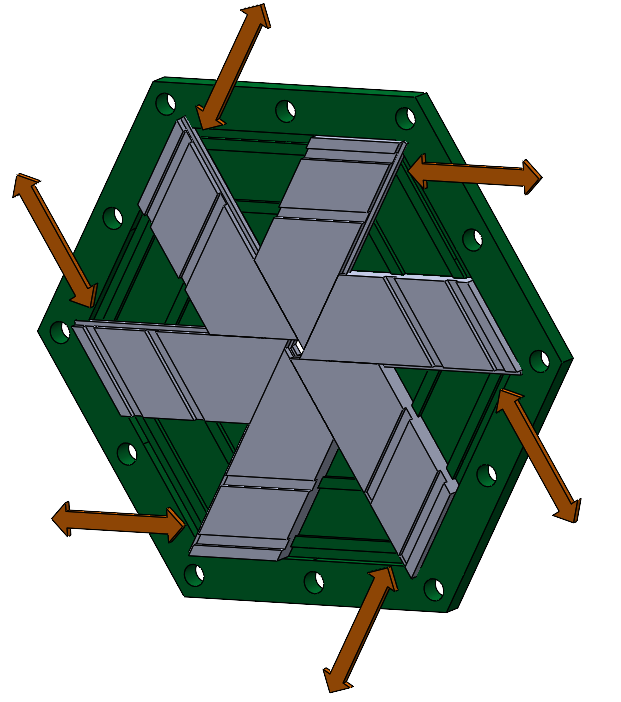
\includegraphics[width=\textwidth]{Hexagon.png}
			\captionof{figure}{Hexagonal diaphragm}
			\label{fig:hexagon}
		\end{minipage}    
		\hfill
		\begin{minipage}[t]{0.45\textwidth}
			\centering
			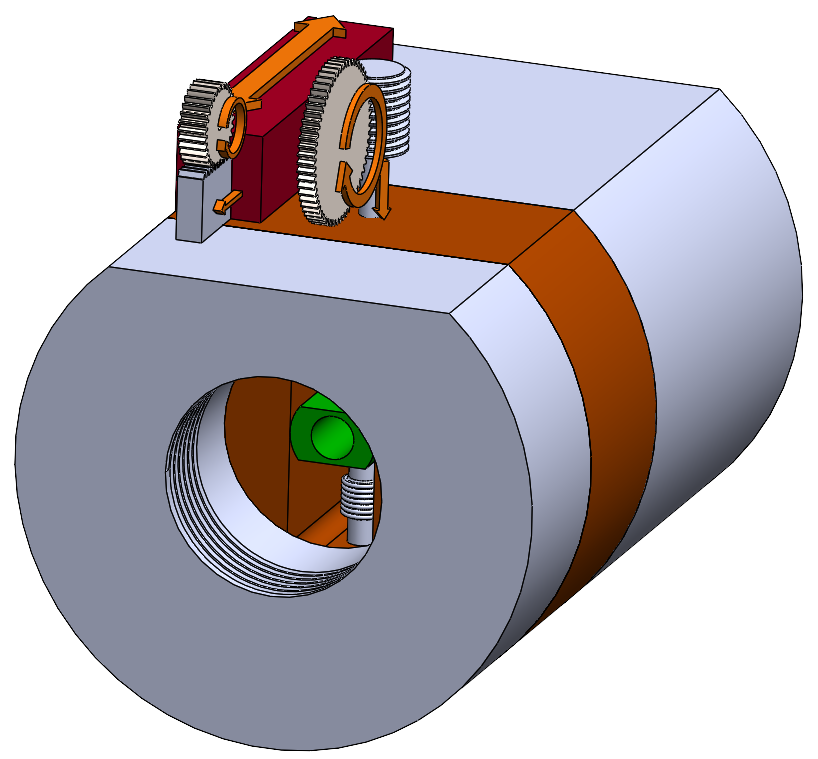
\includegraphics[width=\textwidth]{Gears.png}
			\captionof{figure}{Rack-and-pinion interface}
			\label{fig:gears}
		\end{minipage}    

		\vspace{1em}

		\begin{minipage}[t]{0.45\textwidth}
			\centering
			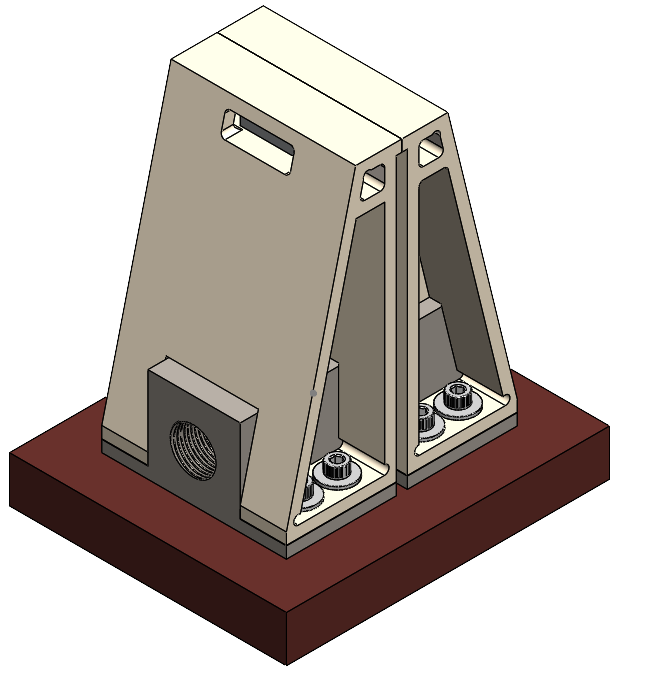
\includegraphics[width=\textwidth]{Mount_trapz.png}
			\captionof{figure}{Direct mount, first iteration}
			\label{fig:trap_mount}
		\end{minipage}    
		\hfill
		\begin{minipage}[t]{0.45\textwidth}
			\centering
			% 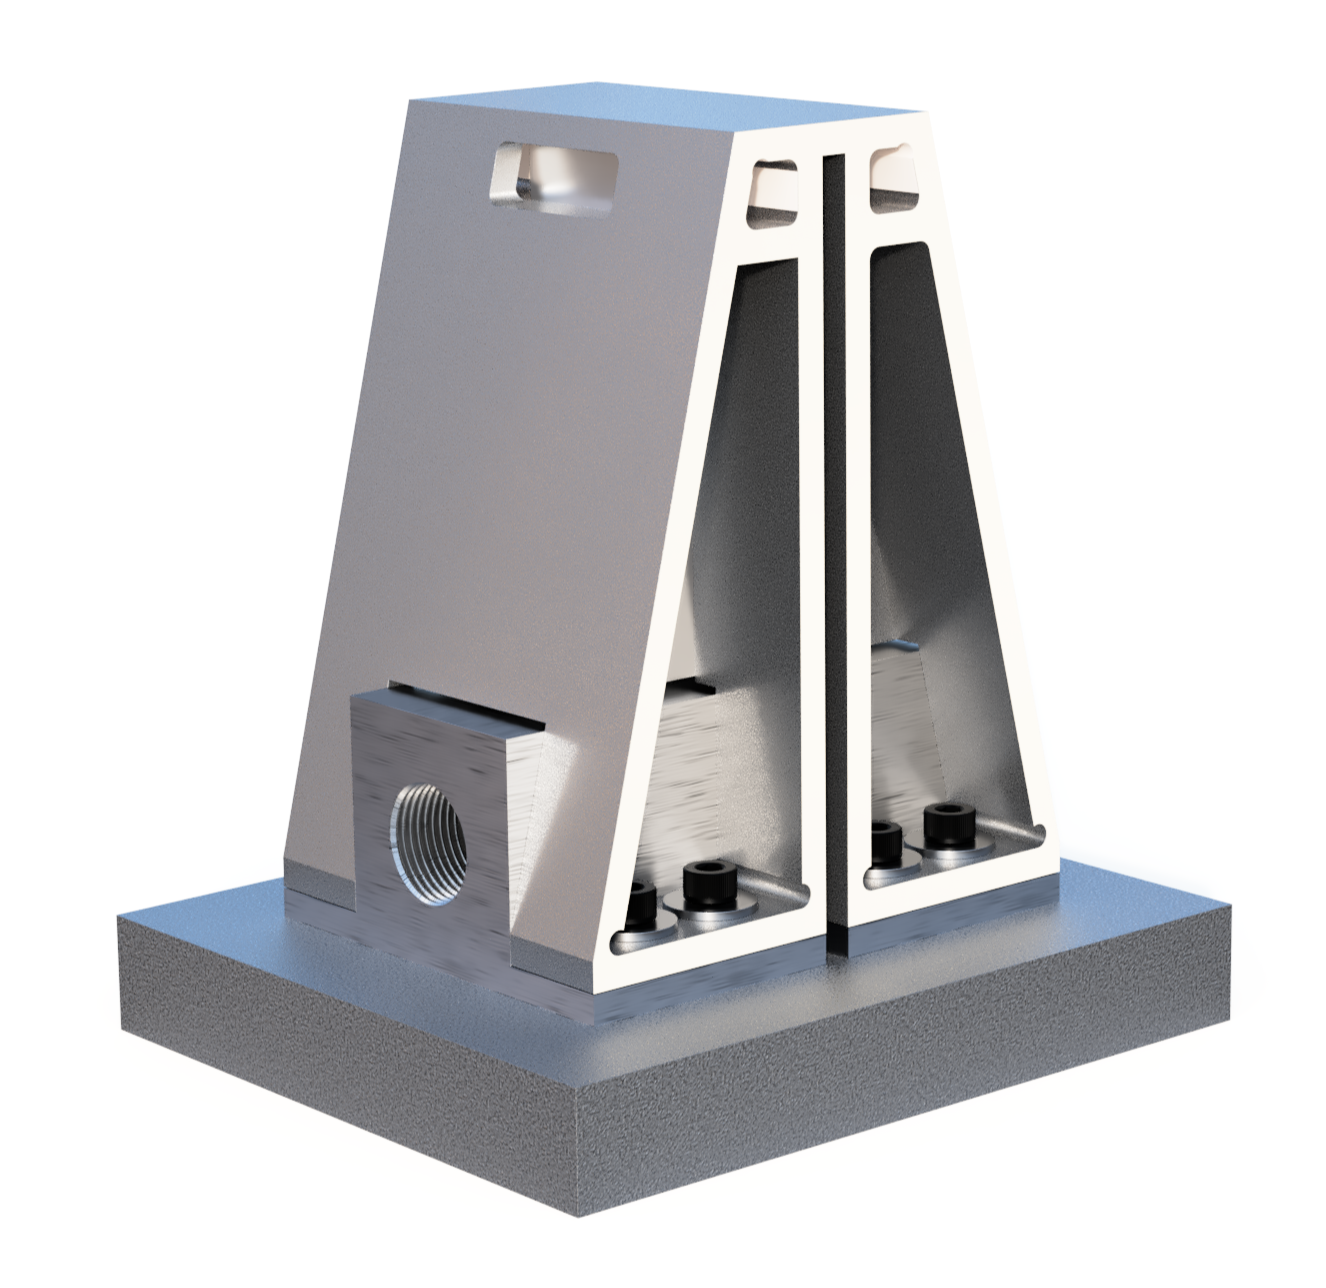
\includegraphics[width=\textwidth]{Complete_Assembly_Render.png}
			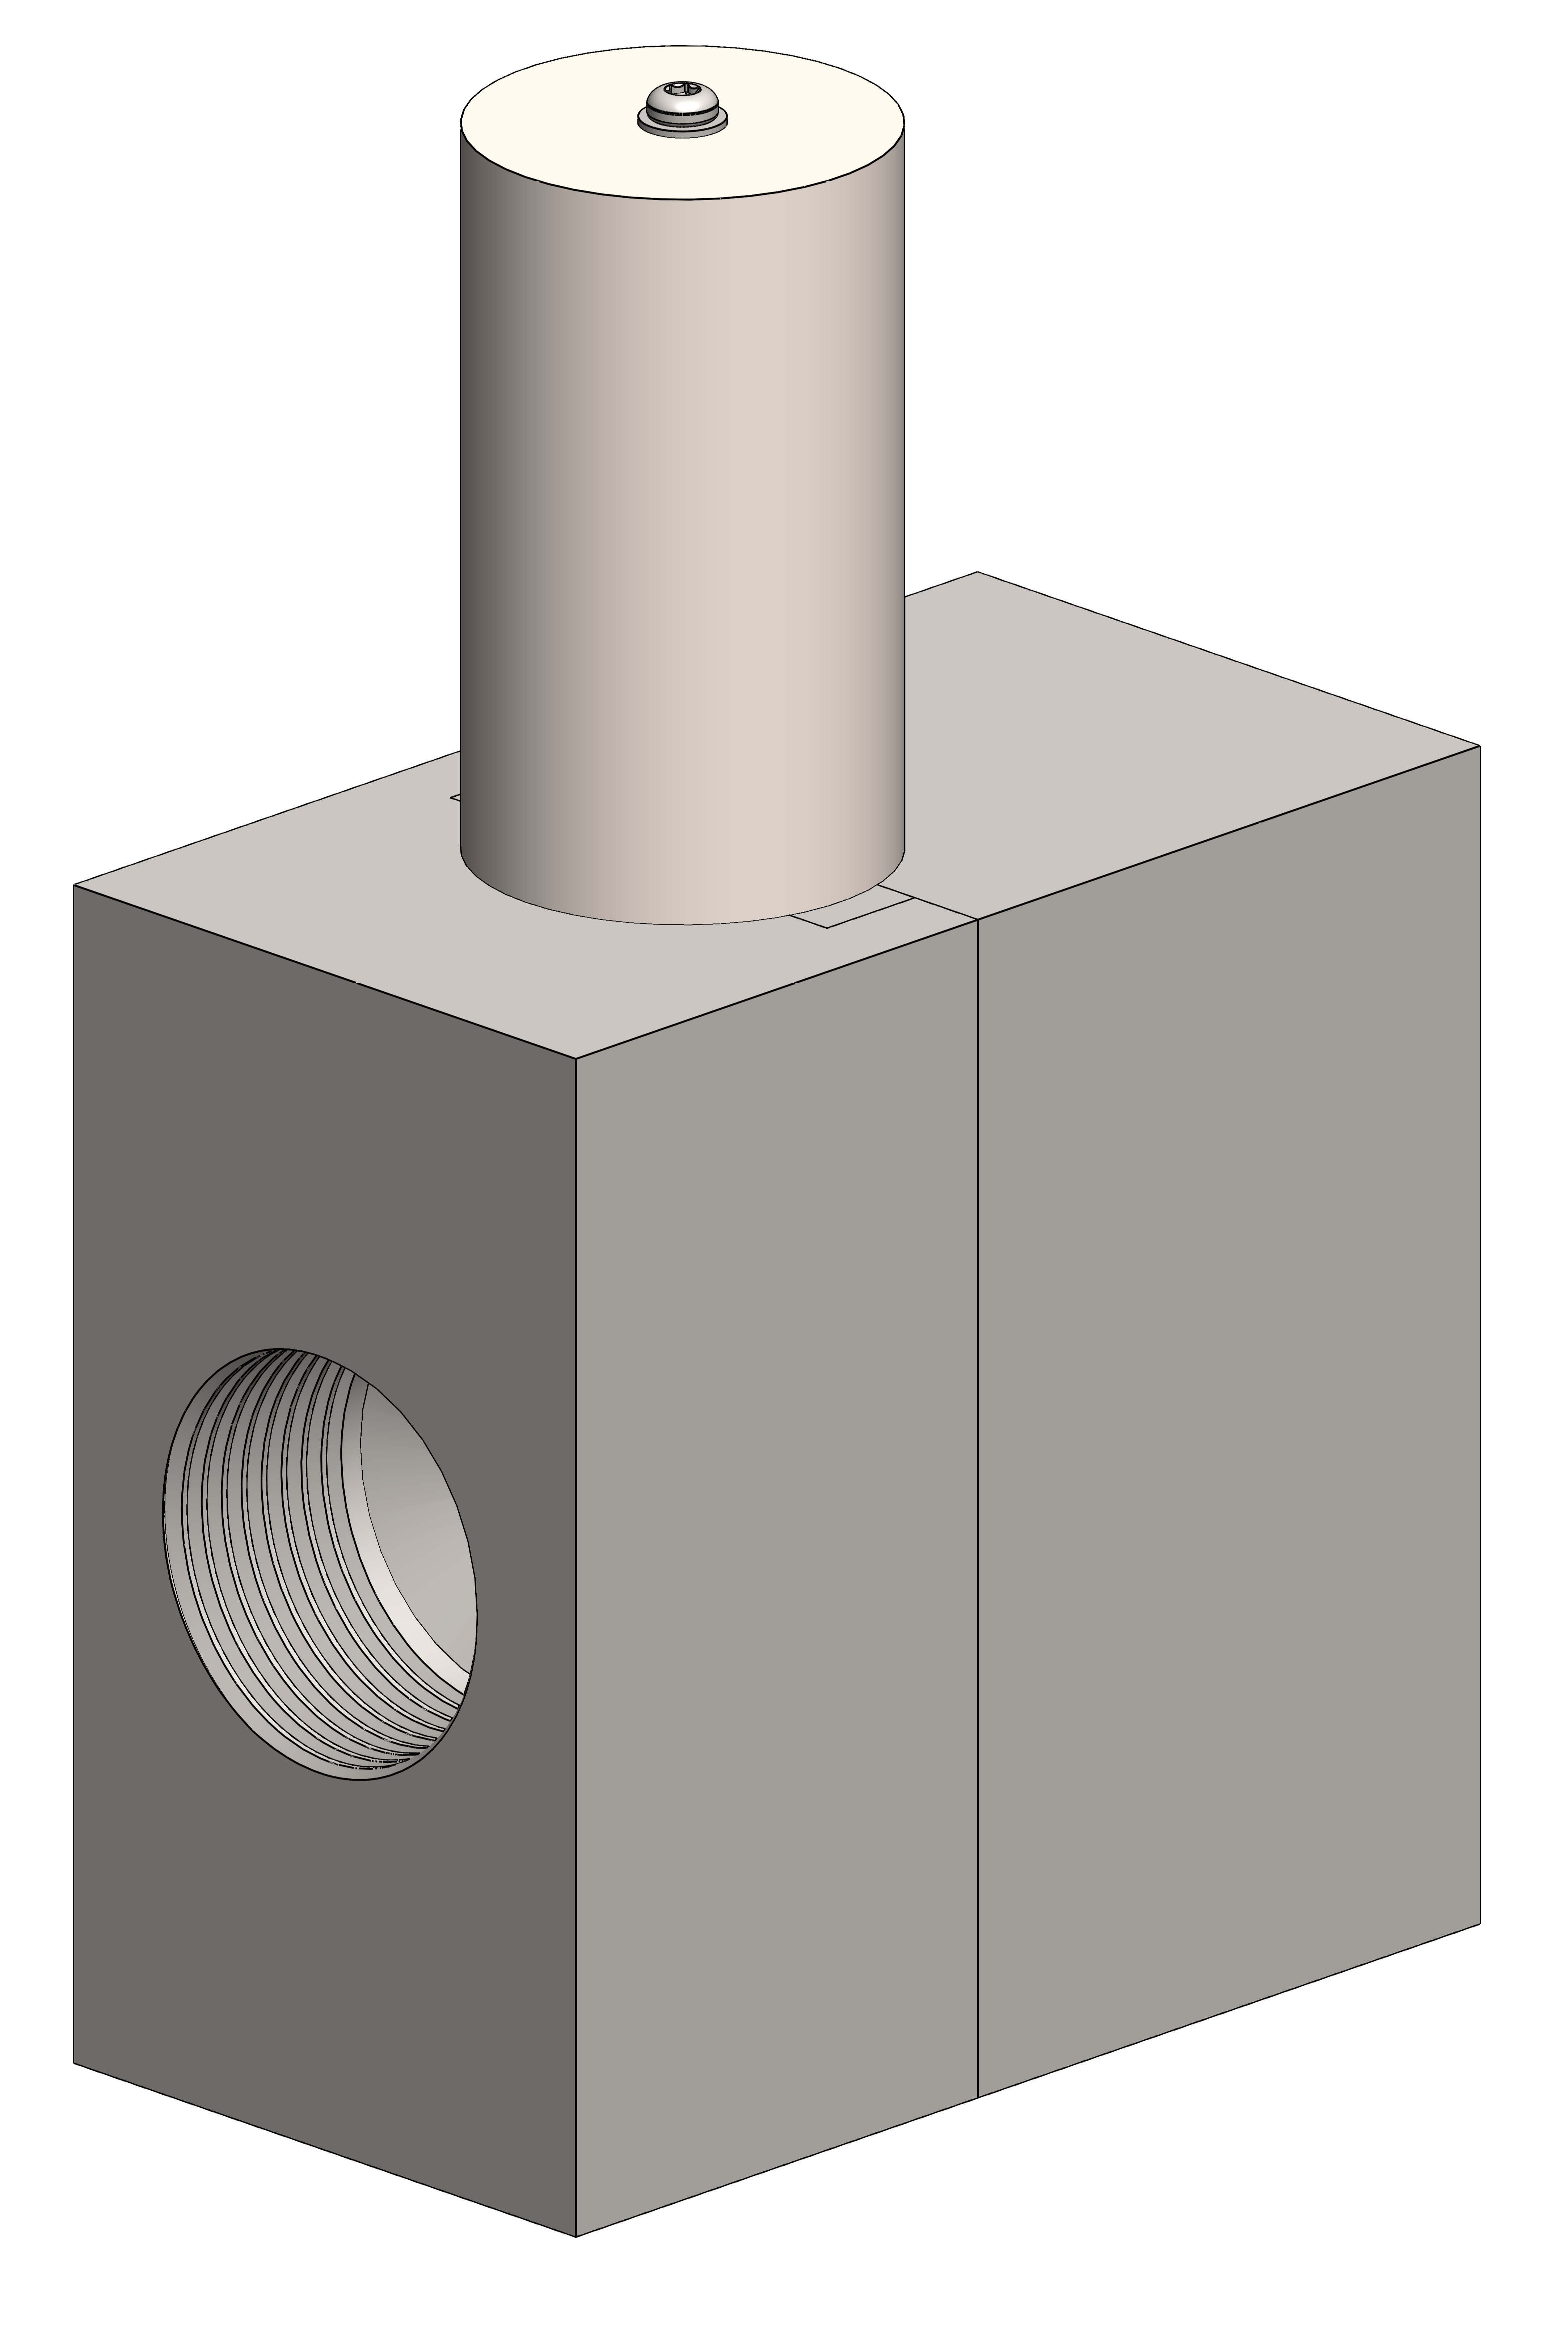
\includegraphics[width=\textwidth]{PTCD.png}
			\captionof{figure}{Final \device\ architecture}
			\label{fig:app_PTCD}
		\end{minipage}    
	\end{figure}    

	\newpage

	\vspace*{.1\textheight}

	\begin{center}

		The authors would like to extend their sincere gratitude to
		Dr. Bradley Bon,\\
		distinguished member of the Gas Transfer Systems team\\
		at Sandia National Laboratories in Livermore, CA\\
		for his invaluable assistance in the development of this design\\

		\vspace*{.05\textheight}

		\textit{Soli Deo Gloria,}\\
		The Noble Aggie Labs\\[24pt]

		\textit{Miguel Cuaycong}\\
		\textit{Jon Pizarro}\\
		\textit{Nicholas Metta}\\
		\textit{Isaiah Mathew}\\
		\textit{John Bodine}\\
		and \textit{Sam van der Veen}

	\end{center}

\end{appendices}

\end{document}